\documentclass[twoside]{book}

% Packages required by doxygen
\usepackage{fixltx2e}
\usepackage{calc}
\usepackage{doxygen}
\usepackage[export]{adjustbox} % also loads graphicx
\usepackage{graphicx}
\usepackage[utf8]{inputenc}
\usepackage{makeidx}
\usepackage{multicol}
\usepackage{multirow}
\PassOptionsToPackage{warn}{textcomp}
\usepackage{textcomp}
\usepackage[nointegrals]{wasysym}
\usepackage[table]{xcolor}

% Font selection
\usepackage[T1]{fontenc}
\usepackage[scaled=.90]{helvet}
\usepackage{courier}
\usepackage{amssymb}
\usepackage{sectsty}
\renewcommand{\familydefault}{\sfdefault}
\allsectionsfont{%
  \fontseries{bc}\selectfont%
  \color{darkgray}%
}
\renewcommand{\DoxyLabelFont}{%
  \fontseries{bc}\selectfont%
  \color{darkgray}%
}
\newcommand{\+}{\discretionary{\mbox{\scriptsize$\hookleftarrow$}}{}{}}

% Page & text layout
\usepackage{geometry}
\geometry{%
  a4paper,%
  top=2.5cm,%
  bottom=2.5cm,%
  left=2.5cm,%
  right=2.5cm%
}
\tolerance=750
\hfuzz=15pt
\hbadness=750
\setlength{\emergencystretch}{15pt}
\setlength{\parindent}{0cm}
\setlength{\parskip}{3ex plus 2ex minus 2ex}
\makeatletter
\renewcommand{\paragraph}{%
  \@startsection{paragraph}{4}{0ex}{-1.0ex}{1.0ex}{%
    \normalfont\normalsize\bfseries\SS@parafont%
  }%
}
\renewcommand{\subparagraph}{%
  \@startsection{subparagraph}{5}{0ex}{-1.0ex}{1.0ex}{%
    \normalfont\normalsize\bfseries\SS@subparafont%
  }%
}
\makeatother

% Headers & footers
\usepackage{fancyhdr}
\pagestyle{fancyplain}
\fancyhead[LE]{\fancyplain{}{\bfseries\thepage}}
\fancyhead[CE]{\fancyplain{}{}}
\fancyhead[RE]{\fancyplain{}{\bfseries\leftmark}}
\fancyhead[LO]{\fancyplain{}{\bfseries\rightmark}}
\fancyhead[CO]{\fancyplain{}{}}
\fancyhead[RO]{\fancyplain{}{\bfseries\thepage}}
\fancyfoot[LE]{\fancyplain{}{}}
\fancyfoot[CE]{\fancyplain{}{}}
\fancyfoot[RE]{\fancyplain{}{\bfseries\scriptsize Generated by Doxygen }}
\fancyfoot[LO]{\fancyplain{}{\bfseries\scriptsize Generated by Doxygen }}
\fancyfoot[CO]{\fancyplain{}{}}
\fancyfoot[RO]{\fancyplain{}{}}
\renewcommand{\footrulewidth}{0.4pt}
\renewcommand{\chaptermark}[1]{%
  \markboth{#1}{}%
}
\renewcommand{\sectionmark}[1]{%
  \markright{\thesection\ #1}%
}

% Indices & bibliography
\usepackage{natbib}
\usepackage[titles]{tocloft}
\setcounter{tocdepth}{3}
\setcounter{secnumdepth}{5}
\makeindex

% Hyperlinks (required, but should be loaded last)
\usepackage{ifpdf}
\ifpdf
  \usepackage[pdftex,pagebackref=true]{hyperref}
\else
  \usepackage[ps2pdf,pagebackref=true]{hyperref}
\fi
\hypersetup{%
  colorlinks=true,%
  linkcolor=blue,%
  citecolor=blue,%
  unicode%
}

% Custom commands
\newcommand{\clearemptydoublepage}{%
  \newpage{\pagestyle{empty}\cleardoublepage}%
}

\usepackage{caption}
\captionsetup{labelsep=space,justification=centering,font={bf},singlelinecheck=off,skip=4pt,position=top}

%===== C O N T E N T S =====

\begin{document}

% Titlepage & ToC
\hypersetup{pageanchor=false,
             bookmarksnumbered=true,
             pdfencoding=unicode
            }
\pagenumbering{alph}
\begin{titlepage}
\vspace*{7cm}
\begin{center}%
{\Large F\+O\+S\+S\+A\+S\+A\+T-\/1B }\\
\vspace*{1cm}
{\large Generated by Doxygen 1.8.13}\\
\end{center}
\end{titlepage}
\clearemptydoublepage
\pagenumbering{roman}
\tableofcontents
\clearemptydoublepage
\pagenumbering{arabic}
\hypersetup{pageanchor=true}

%--- Begin generated contents ---
\chapter{Main Page}
\label{index}\hypertarget{index}{}\section*{N\+O\+T\+I\+CE}

The tests given here are only guidelines, please also refer to the F\+O\+S\+S\+A\+S\+A\+T-\/1 software test plans and documentation for a complete view.

\section*{Navigation}


\begin{DoxyItemize}
\item See the modules section for help with the satellite\textquotesingle{}s configuration.
\item Each header file contains documentation. 
\end{DoxyItemize}
\chapter{Test List}
\label{test}
\Hypertarget{test}

\begin{DoxyRefList}
\item[\label{test__test000009}%
\Hypertarget{test__test000009}%
Global \hyperlink{communication_8h_a03f49b9aabc52b55893829b7069efc7b}{Communication\+\_\+\+Acknowledge} (uint8\+\_\+t function\+Id, uint8\+\_\+t result)](ID C\+O\+M\+M\+S\+\_\+\+H\+\_\+\+T10) (S\+EV 1) Test that each command/packet is processed correctly. 
\item[\label{test__test000015}%
\Hypertarget{test__test000015}%
Global \hyperlink{communication_8h_abe2c8a0d33c8d6a33fe6fd33c729a5a9}{Communication\+\_\+\+Check\+\_\+\+Opt\+Data\+Len} (uint8\+\_\+t expected, uint8\+\_\+t actual)](ID C\+O\+M\+M\+S\+\_\+\+H\+\_\+\+T14) (S\+EV 1) Check that this function equates correctly. 
\item[\label{test__test000006}%
\Hypertarget{test__test000006}%
Global \hyperlink{communication_8h_aee0a3df78da4459c808120a803c65b61}{Communication\+\_\+\+C\+W\+\_\+\+Beep} (uint32\+\_\+t len)](ID C\+O\+M\+M\+S\+\_\+\+H\+\_\+\+T7) (S\+EV 2) Test that the CW beep is received ok. 
\item[\label{test__test000012}%
\Hypertarget{test__test000012}%
Global \hyperlink{communication_8h_a834526d017e482716c6061772d644d5b}{Communication\+\_\+\+Execute\+\_\+\+Function} (uint8\+\_\+t function\+Id, uint8\+\_\+t $\ast$opt\+Data=N\+U\+LL, size\+\_\+t opt\+Data\+Len=0)](ID C\+O\+M\+M\+S\+\_\+\+H\+\_\+\+T11) (S\+EV 1) Test that each command is responded to with the correct function and data. 
\item[\label{test__test000007}%
\Hypertarget{test__test000007}%
Global \hyperlink{communication_8h_a980dd25e42aaeac1620dc7f9b42859a2}{Communication\+\_\+\+Frame\+\_\+\+Add} (uint8\+\_\+t $\ast$$\ast$buff\+Ptr, T val, const char $\ast$name, uint32\+\_\+t mult, const char $\ast$unit)](ID C\+O\+M\+M\+S\+\_\+\+H\+\_\+\+T8) (S\+EV 1) Test that the system information is received correctly. 
\item[\label{test__test000010}%
\Hypertarget{test__test000010}%
Global \hyperlink{communication_8h_ad5052f7320724c62bfab348ea62c66ce}{Communication\+\_\+\+Process\+\_\+\+Packet} ()](ID C\+O\+M\+M\+S\+\_\+\+H\+\_\+\+T9) (S\+EV 1) Test that each command/packet is processed correctly. 
\item[\label{test__test000001}%
\Hypertarget{test__test000001}%
Global \hyperlink{communication_8h_aaadcd86dea525de318e35078c63b3149}{Communication\+\_\+\+Receive\+\_\+\+Interrupt} ()](ID C\+O\+M\+M\+S\+\_\+\+H\+\_\+\+T0) (S\+EV 1) Make sure this function is called when the radio receives data. 
\item[\label{test__test000005}%
\Hypertarget{test__test000005}%
Global \hyperlink{communication_8h_a5db7440be24bedc9c14f12db46029968}{Communication\+\_\+\+Send\+\_\+\+Morse\+\_\+\+Beacon} (float batt\+Voltage)](ID C\+O\+M\+M\+S\+\_\+\+H\+\_\+\+T5) (S\+EV 1) Test that the beacon message can be received properly. 

(ID C\+O\+M\+M\+S\+\_\+\+H\+\_\+\+T6) (S\+EV 1) Test that the beacon messages battery voltage is received ok. 
\item[\label{test__test000013}%
\Hypertarget{test__test000013}%
Global \hyperlink{communication_8h_af86331e2820ea70a7928919915937077}{Communication\+\_\+\+Send\+\_\+\+Response} (uint8\+\_\+t resp\+Id, uint8\+\_\+t $\ast$opt\+Data=nullptr, size\+\_\+t opt\+Data\+Len=0, bool override\+Modem=false)](ID C\+O\+M\+M\+S\+\_\+\+H\+\_\+\+T12) (S\+EV 1) Test that each response transmits correctly. 
\item[\label{test__test000008}%
\Hypertarget{test__test000008}%
Global \hyperlink{communication_8h_ae4e350e62342431fda2184ff0dc47a65}{Communication\+\_\+\+Send\+\_\+\+System\+\_\+\+Info} ()](ID C\+O\+M\+M\+S\+\_\+\+H\+\_\+\+T8) (S\+EV 1) Test that the system information is received correctly. 
\item[\label{test__test000003}%
\Hypertarget{test__test000003}%
Global \hyperlink{communication_8h_a59478c57f2735f94bf2f19a272a75c02}{Communication\+\_\+\+Set\+\_\+\+Configuration} (uint8\+\_\+t $\ast$opt\+Data, uint8\+\_\+t opt\+Data\+Len)](ID C\+O\+M\+M\+S\+\_\+\+H\+\_\+\+T2) (S\+EV 1) Make sure the modem mode is changed with no errors. 
\item[\label{test__test000002}%
\Hypertarget{test__test000002}%
Global \hyperlink{communication_8h_a0183d47f45dfdb348647c3db1a75b73c}{Communication\+\_\+\+Set\+\_\+\+Modem} (uint8\+\_\+t modem)](ID C\+O\+M\+M\+S\+\_\+\+H\+\_\+\+T1) (S\+EV 1) Make sure the modem mode is changed with no errors. 
\item[\label{test__test000004}%
\Hypertarget{test__test000004}%
Global \hyperlink{communication_8h_ad184c979eb82cc1c8d4fc32a802cb758}{Communication\+\_\+\+Set\+\_\+\+Spreading\+Factor} (uint8\+\_\+t sf\+Mode)](ID C\+O\+M\+M\+S\+\_\+\+H\+\_\+\+T3) (S\+EV 1) Make sure the radio\textquotesingle{}s spreading factor can be changed with no errors. 

(ID C\+O\+M\+M\+S\+\_\+\+H\+\_\+\+T4) (S\+EV 1) Make sure the radio\textquotesingle{}s spreading factors are compatable with generic radios. 
\item[\label{test__test000014}%
\Hypertarget{test__test000014}%
Global \hyperlink{communication_8h_a46802cdf83e9de4cab3ebd4a00256aeb}{Communication\+\_\+\+Transmit} (uint8\+\_\+t $\ast$data, uint8\+\_\+t len, bool override\+Modem=true)](ID C\+O\+M\+M\+S\+\_\+\+H\+\_\+\+T13) (S\+EV 1) Check that each function/command transmits correctly. 
\item[\label{test__test000011}%
\Hypertarget{test__test000011}%
Global \hyperlink{communication_8h_ab6495de804d5d54d071fe8b4dd408aba}{Comunication\+\_\+\+Parse\+\_\+\+Frame} (uint8\+\_\+t $\ast$frame, size\+\_\+t len)](ID C\+O\+M\+M\+S\+\_\+\+H\+\_\+\+T10) (S\+EV 1) Test that each command/packet is processed correctly. 
\item[\label{test__test000016}%
\Hypertarget{test__test000016}%
Module \hyperlink{group__defines__debug__macros}{defines\+\_\+debug\+\_\+macros} ](ID C\+O\+N\+F\+\_\+\+D\+E\+B\+U\+G\+\_\+\+M\+A\+C\+R\+O\+S\+\_\+\+T0) (S\+EV 1) Uncomment E\+N\+A\+B\+L\+E\+\_\+\+T\+R\+A\+N\+S\+M\+I\+S\+S\+I\+O\+N\+\_\+\+C\+O\+N\+T\+R\+OL, test no transmissions are produced. 

(ID C\+O\+N\+F\+\_\+\+D\+E\+B\+U\+G\+\_\+\+M\+A\+C\+R\+O\+S\+\_\+\+T1) (S\+EV 1) Uncomment E\+N\+A\+B\+L\+E\+\_\+\+D\+E\+P\+L\+O\+Y\+M\+E\+N\+T\+\_\+\+S\+E\+Q\+U\+E\+N\+CE, test no deployment sequence ran (this define is for debugging purposes). 

(ID C\+O\+N\+F\+\_\+\+D\+E\+B\+U\+G\+\_\+\+M\+A\+C\+R\+O\+S\+\_\+\+T2) (S\+EV 1) Uncomment E\+N\+A\+B\+L\+E\+\_\+\+I\+N\+T\+E\+R\+V\+A\+L\+\_\+\+C\+O\+N\+T\+R\+OL, test that the battery voltages have no affect on the sleep duration. 

(ID C\+O\+N\+F\+\_\+\+D\+E\+B\+U\+G\+\_\+\+M\+A\+C\+R\+O\+S\+\_\+\+T3) (S\+EV 1) Uncomment E\+N\+A\+B\+L\+E\+\_\+\+I\+N\+A226, test that the current readings are correct. 
\item[\label{test__test000018}%
\Hypertarget{test__test000018}%
Module \hyperlink{group__defines__default__power__configuration}{defines\+\_\+default\+\_\+power\+\_\+configuration} ](ID C\+O\+N\+F\+\_\+\+P\+O\+W\+E\+R\+\_\+\+C\+O\+N\+F\+\_\+\+T0) (S\+EV 1) Check that the low power mode works. 

(ID C\+O\+N\+F\+\_\+\+P\+O\+W\+E\+R\+\_\+\+C\+O\+N\+F\+\_\+\+T1) (S\+EV 1) Check that the low power mode can be disabled using L\+O\+W\+\_\+\+P\+O\+W\+E\+R\+\_\+\+M\+O\+D\+E\+\_\+\+E\+N\+A\+B\+L\+ED. 

(ID C\+O\+N\+F\+\_\+\+P\+O\+W\+E\+R\+\_\+\+C\+O\+N\+F\+\_\+\+T3) (S\+EV 1) Check that the M\+P\+PT is controlled by the temperature using M\+P\+P\+T\+\_\+\+T\+E\+M\+P\+\_\+\+S\+W\+I\+T\+C\+H\+\_\+\+E\+N\+A\+B\+L\+ED. 

(ID C\+O\+N\+F\+\_\+\+P\+O\+W\+E\+R\+\_\+\+C\+O\+N\+F\+\_\+\+T4) (S\+EV 1) Check that the M\+P\+PT\textquotesingle{}s temperature controller can be disabled and enabled using M\+P\+P\+T\+\_\+\+K\+E\+E\+P\+\_\+\+A\+L\+I\+V\+E\+\_\+\+E\+N\+A\+B\+L\+ED. 

(ID C\+O\+N\+F\+\_\+\+P\+O\+W\+E\+R\+\_\+\+C\+O\+N\+F\+\_\+\+T5) (S\+EV 1) Check that the satellite\textquotesingle{}s transmissions can be disabled and enabled using T\+R\+A\+N\+S\+M\+I\+T\+\_\+\+E\+N\+A\+B\+L\+ED. 
\item[\label{test__test000020}%
\Hypertarget{test__test000020}%
Module \hyperlink{group__defines__eeprom__address__map}{defines\+\_\+eeprom\+\_\+address\+\_\+map} ](ID C\+O\+N\+F\+\_\+\+E\+E\+P\+R\+O\+M\+\_\+\+A\+D\+D\+R\+\_\+\+M\+A\+P\+\_\+\+T0) (S\+EV 1) Check that E\+E\+P\+R\+O\+M\+\_\+\+D\+E\+P\+L\+O\+Y\+M\+E\+N\+T\+\_\+\+C\+O\+U\+N\+T\+E\+R\+\_\+\+A\+D\+DR is functional, including restarts. 

(ID C\+O\+N\+F\+\_\+\+E\+E\+P\+R\+O\+M\+\_\+\+A\+D\+D\+R\+\_\+\+M\+A\+P\+\_\+\+T1) (S\+EV 1) Check that E\+E\+P\+R\+O\+M\+\_\+\+P\+O\+W\+E\+R\+\_\+\+C\+O\+N\+F\+I\+G\+\_\+\+A\+D\+DR is functional, including restarts. 

(ID C\+O\+N\+F\+\_\+\+E\+E\+P\+R\+O\+M\+\_\+\+A\+D\+D\+R\+\_\+\+M\+A\+P\+\_\+\+T2) (S\+EV 1) Check that E\+E\+P\+R\+O\+M\+\_\+\+F\+I\+R\+S\+T\+\_\+\+R\+U\+N\+\_\+\+A\+D\+DR is functional, including restarts. 

(ID C\+O\+N\+F\+\_\+\+E\+E\+P\+R\+O\+M\+\_\+\+A\+D\+D\+R\+\_\+\+M\+A\+P\+\_\+\+T3) (S\+EV 1) Check that E\+E\+P\+R\+O\+M\+\_\+\+R\+E\+S\+T\+A\+R\+T\+\_\+\+C\+O\+U\+N\+T\+E\+R\+\_\+\+A\+D\+DR is functional, including restarts. 

(ID C\+O\+N\+F\+\_\+\+E\+E\+P\+R\+O\+M\+\_\+\+A\+D\+D\+R\+\_\+\+M\+A\+P\+\_\+\+T4) (S\+EV 1) Check that E\+E\+P\+R\+O\+M\+\_\+\+C\+A\+L\+L\+S\+I\+G\+N\+\_\+\+L\+E\+N\+\_\+\+A\+D\+DR is functional, including restarts. 

(ID C\+O\+N\+F\+\_\+\+E\+E\+P\+R\+O\+M\+\_\+\+A\+D\+D\+R\+\_\+\+M\+A\+P\+\_\+\+T5) (S\+EV 1) Check that E\+E\+P\+R\+O\+M\+\_\+\+C\+A\+L\+L\+S\+I\+G\+N\+\_\+\+A\+D\+DR is functional, including restarts. 
\item[\label{test__test000021}%
\Hypertarget{test__test000021}%
Module \hyperlink{group__defines__eeprom__variables}{defines\+\_\+eeprom\+\_\+variables} ](ID C\+O\+N\+F\+\_\+\+E\+E\+P\+R\+O\+M\+\_\+\+V\+A\+R\+\_\+\+T0) (S\+EV 1) Check that the E\+E\+P\+R\+O\+M\+\_\+\+R\+E\+S\+E\+T\+\_\+\+V\+A\+L\+UE is suitable. 

(ID C\+O\+N\+F\+\_\+\+E\+E\+P\+R\+O\+M\+\_\+\+V\+A\+R\+\_\+\+T1) (S\+EV 1) Check that the E\+E\+P\+R\+O\+M\+\_\+\+F\+I\+R\+S\+T\+\_\+\+R\+UN is suitable. 

(ID C\+O\+N\+F\+\_\+\+E\+E\+P\+R\+O\+M\+\_\+\+V\+A\+R\+\_\+\+T3) (S\+EV 1) Check that the E\+E\+P\+R\+O\+M\+\_\+\+C\+O\+N\+S\+E\+C\+U\+T\+I\+V\+E\+\_\+\+R\+UN is suitable. 
\item[\label{test__test000019}%
\Hypertarget{test__test000019}%
Module \hyperlink{group__defines__ina226__configuration}{defines\+\_\+ina226\+\_\+configuration} ](ID C\+O\+N\+F\+\_\+\+I\+N\+A226\+\_\+\+C\+O\+N\+F\+\_\+\+T0) (S\+EV 1) Check that the I\+N\+A226 can be connected to and gives the correct values. 
\item[\label{test__test000024}%
\Hypertarget{test__test000024}%
Module \hyperlink{group__defines__mcu__temperature__configuration}{defines\+\_\+mcu\+\_\+temperature\+\_\+configuration} ](ID C\+O\+N\+F\+\_\+\+M\+C\+U\+\_\+\+T\+E\+M\+P\+\_\+\+T0) (S\+EV 1) Check that the M\+C\+U\+\_\+\+T\+E\+M\+P\+\_\+\+O\+F\+F\+S\+ET functions correctly. 

(ID C\+O\+N\+F\+\_\+\+M\+C\+U\+\_\+\+T\+E\+M\+P\+\_\+\+T1) (S\+EV 1) Check that the M\+C\+U\+\_\+\+T\+E\+M\+P\+\_\+\+C\+O\+E\+F\+F\+I\+C\+I\+E\+NT functions correctly. 
\item[\label{test__test000022}%
\Hypertarget{test__test000022}%
Module \hyperlink{group__defines__pin__map}{defines\+\_\+pin\+\_\+map} ](ID C\+O\+N\+F\+\_\+\+P\+I\+N\+\_\+\+M\+A\+P\+\_\+\+T0) (S\+EV 1) Check that solar panel A voltage can be read from A\+N\+A\+L\+O\+G\+\_\+\+I\+N\+\_\+\+S\+O\+L\+A\+R\+\_\+\+A\+\_\+\+V\+O\+L\+T\+A\+G\+E\+\_\+\+P\+IN. 

(ID C\+O\+N\+F\+\_\+\+P\+I\+N\+\_\+\+M\+A\+P\+\_\+\+T1) (S\+EV 1) Check that solar panel B voltage can be read from A\+N\+A\+L\+O\+G\+\_\+\+I\+N\+\_\+\+S\+O\+L\+A\+R\+\_\+\+B\+\_\+\+V\+O\+L\+T\+A\+G\+E\+\_\+\+P\+IN. 

(ID C\+O\+N\+F\+\_\+\+P\+I\+N\+\_\+\+M\+A\+P\+\_\+\+T2) (S\+EV 1) Check that solar panel C voltage can be read from A\+N\+A\+L\+O\+G\+\_\+\+I\+N\+\_\+\+S\+O\+L\+A\+R\+\_\+\+C\+\_\+\+V\+O\+L\+T\+A\+G\+E\+\_\+\+P\+IN. 

(ID C\+O\+N\+F\+\_\+\+P\+I\+N\+\_\+\+M\+A\+P\+\_\+\+T3) (S\+EV 1) Check that the random seed analog pin is suitable from A\+N\+A\+L\+O\+G\+\_\+\+I\+N\+\_\+\+R\+A\+N\+D\+O\+M\+\_\+\+S\+E\+ED. 

(ID C\+O\+N\+F\+\_\+\+P\+I\+N\+\_\+\+M\+A\+P\+\_\+\+T4) (S\+EV 1) Check that the M\+P\+PT circuit is controlled correctly using D\+I\+G\+I\+T\+A\+L\+\_\+\+O\+U\+T\+\_\+\+M\+P\+P\+T\+\_\+\+P\+IN. 

(ID C\+O\+N\+F\+\_\+\+P\+I\+N\+\_\+\+M\+A\+P\+\_\+\+T5) (S\+EV 1) Check that the deployment hardware deploys when D\+I\+G\+I\+T\+A\+L\+\_\+\+O\+U\+T\+\_\+\+M\+O\+S\+F\+E\+T\+\_\+1 and D\+I\+G\+I\+T\+A\+L\+\_\+\+O\+U\+T\+\_\+\+M\+O\+S\+F\+E\+T\+\_\+2 are brought high. 

(ID C\+O\+N\+F\+\_\+\+P\+I\+N\+\_\+\+M\+A\+P\+\_\+\+T6) (S\+EV 1) Check that the radio can be communicated with using pins R\+A\+D\+I\+O\+\_\+\+N\+SS, R\+A\+D\+I\+O\+\_\+\+D\+I\+O1, R\+A\+D\+I\+O\+\_\+\+B\+U\+SY and R\+A\+D\+I\+O\+\_\+\+N\+R\+ST. 
\item[\label{test__test000017}%
\Hypertarget{test__test000017}%
Module \hyperlink{group__defines__power__management__configuration}{defines\+\_\+power\+\_\+management\+\_\+configuration} ](ID C\+O\+N\+F\+\_\+\+P\+O\+W\+E\+R\+\_\+\+M\+A\+N\+A\+G\+E\+M\+E\+N\+T\+\_\+\+T0) (S\+EV 1) Check that the satellite switches to low power mode when its voltage goes below B\+A\+T\+T\+E\+R\+Y\+\_\+\+V\+O\+L\+T\+A\+G\+E\+\_\+\+L\+I\+M\+IT. 

(ID C\+O\+N\+F\+\_\+\+P\+O\+W\+E\+R\+\_\+\+M\+A\+N\+A\+G\+E\+M\+E\+N\+T\+\_\+\+T1) (S\+EV 2) Check that the satellite sends a morse beacon transmission when it switches to Low Power Mode. 

(ID C\+O\+N\+F\+\_\+\+P\+O\+W\+E\+R\+\_\+\+M\+A\+N\+A\+G\+E\+M\+E\+N\+T\+\_\+\+T2) (S\+EV 1) Check that the battery stops charging when the temperature goes below this threshold, and starts charging again when it is not. 

(ID C\+O\+N\+F\+\_\+\+P\+O\+W\+E\+R\+\_\+\+M\+A\+N\+A\+G\+E\+M\+E\+N\+T\+\_\+\+T3) (S\+EV 1) Check that the watchdog is signalled every W\+A\+T\+C\+H\+D\+O\+G\+\_\+\+L\+O\+O\+P\+\_\+\+H\+E\+A\+R\+T\+B\+E\+A\+T\+\_\+\+P\+E\+R\+I\+OD. 

(ID C\+O\+N\+F\+\_\+\+P\+O\+W\+E\+R\+\_\+\+M\+A\+N\+A\+G\+E\+M\+E\+N\+T\+\_\+\+T4) (S\+EV 1) Check that the satellite sleeping times using the S\+L\+E\+E\+P\+\_\+\+L\+E\+N\+G\+T\+H\+\_\+\+C\+O\+N\+S\+T\+A\+NT is suitable to account for the Low\+Power libraries overhead. 

(ID C\+O\+N\+F\+\_\+\+P\+O\+W\+E\+R\+\_\+\+M\+A\+N\+A\+G\+E\+M\+E\+N\+T\+\_\+\+T5) (S\+EV 1) Check that the satellite does not deploy after D\+E\+P\+L\+O\+Y\+M\+E\+N\+T\+\_\+\+A\+T\+T\+E\+M\+PS has reached. 

(ID C\+O\+N\+F\+\_\+\+P\+O\+W\+E\+R\+\_\+\+M\+A\+N\+A\+G\+E\+M\+E\+N\+T\+\_\+\+T6) (S\+EV 1) Check that the satellite waits for this amount of time before the deploy sequence starts, this is for jettison. 

(ID C\+O\+N\+F\+\_\+\+P\+O\+W\+E\+R\+\_\+\+M\+A\+N\+A\+G\+E\+M\+E\+N\+T\+\_\+\+T7) (S\+EV 5) Check that each debug print waits D\+E\+P\+L\+O\+Y\+M\+E\+N\+T\+\_\+\+D\+E\+B\+U\+G\+\_\+\+S\+A\+M\+P\+L\+E\+\_\+\+P\+E\+R\+I\+OD amount of time between each print. 
\item[\label{test__test000025}%
\Hypertarget{test__test000025}%
Module \hyperlink{group__defines__radio__common__configuraiton}{defines\+\_\+radio\+\_\+common\+\_\+configuraiton} ](ID C\+O\+N\+F\+\_\+\+R\+A\+D\+I\+O\+\_\+\+T0) (S\+EV 1) Check that the S\+Y\+N\+C\+\_\+\+W\+O\+RD is compatable with all radios and is suitable. 

(ID C\+O\+N\+F\+\_\+\+R\+A\+D\+I\+O\+\_\+\+T1) (S\+EV 1) Check that the T\+X\+C0\+\_\+\+V\+O\+L\+T\+A\+GE value is suitable. 

(ID C\+O\+N\+F\+\_\+\+R\+A\+D\+I\+O\+\_\+\+T2) (S\+EV 1) Check that the L\+O\+W\+\_\+\+P\+O\+W\+E\+R\+\_\+\+L\+E\+V\+EL is suitable. 

(ID C\+O\+N\+F\+\_\+\+R\+A\+D\+I\+O\+\_\+\+T3) (S\+EV 1) Check that the M\+A\+X\+\_\+\+N\+U\+M\+B\+E\+R\+\_\+\+O\+F\+\_\+\+B\+L\+O\+C\+KS works. 

(ID C\+O\+N\+F\+\_\+\+R\+A\+D\+I\+O\+\_\+\+T4) (S\+EV 1) Check that the L\+O\+R\+A\+\_\+\+R\+E\+C\+E\+I\+V\+E\+\_\+\+W\+I\+N\+D\+O\+W\+\_\+\+L\+E\+N\+G\+TH works. 

(ID C\+O\+N\+F\+\_\+\+R\+A\+D\+I\+O\+\_\+\+T5) (S\+EV 1) Check that the F\+S\+K\+\_\+\+R\+E\+C\+E\+I\+V\+E\+\_\+\+W\+I\+N\+D\+O\+W\+\_\+\+L\+E\+N\+G\+TH works. 

(ID C\+O\+N\+F\+\_\+\+R\+A\+D\+I\+O\+\_\+\+T6) (S\+EV 1) Check that the R\+E\+S\+P\+O\+N\+S\+E\+\_\+\+D\+E\+L\+AY is suitable and works. 
\item[\label{test__test000026}%
\Hypertarget{test__test000026}%
Module \hyperlink{group__defines__radio__lora__configuration}{defines\+\_\+radio\+\_\+lora\+\_\+configuration} ]Test that we can receive Lo\+Ra transmissions from the satellite with these default parameters 

(ID C\+O\+N\+F\+\_\+\+L\+O\+R\+A\+\_\+\+R\+A\+D\+I\+O\+\_\+\+T1) (S\+EV 1) Check that the radio transmits at L\+O\+R\+A\+\_\+\+B\+A\+N\+D\+W\+I\+D\+TH. 

(ID C\+O\+N\+F\+\_\+\+L\+O\+R\+A\+\_\+\+R\+A\+D\+I\+O\+\_\+\+T2) (S\+EV 1) Check that the radio is transmitting at L\+O\+R\+A\+\_\+\+S\+P\+R\+E\+A\+D\+I\+N\+G\+\_\+\+F\+A\+C\+T\+OR. 

(ID C\+O\+N\+F\+\_\+\+L\+O\+R\+A\+\_\+\+R\+A\+D\+I\+O\+\_\+\+T3) (S\+EV 1) Check that the radio can/is transmitting at L\+O\+R\+A\+\_\+\+S\+P\+R\+E\+A\+D\+I\+N\+G\+\_\+\+F\+A\+C\+T\+O\+R\+\_\+\+A\+LT. 

(ID C\+O\+N\+F\+\_\+\+L\+O\+R\+A\+\_\+\+R\+A\+D\+I\+O\+\_\+\+T4) (S\+EV 1) Check that the radio is transmitting at L\+O\+R\+A\+\_\+\+C\+O\+D\+I\+N\+G\+\_\+\+R\+A\+TE. 

(ID C\+O\+N\+F\+\_\+\+L\+O\+R\+A\+\_\+\+R\+A\+D\+I\+O\+\_\+\+T5) (S\+EV 1) Check that the radio is transmitting at L\+O\+R\+A\+\_\+\+O\+U\+T\+P\+U\+T\+\_\+\+P\+O\+W\+ER. 

(ID C\+O\+N\+F\+\_\+\+L\+O\+R\+A\+\_\+\+R\+A\+D\+I\+O\+\_\+\+T6) (S\+EV 1) Check that the radio draws no more than 160.\+0mA.

(ID C\+O\+N\+F\+\_\+\+L\+O\+R\+A\+\_\+\+R\+A\+D\+I\+O\+\_\+\+T0) (S\+EV 1) Check that the radio transmits lora at L\+O\+R\+A\+\_\+\+C\+A\+R\+R\+I\+E\+R\+\_\+\+F\+R\+E\+Q\+U\+E\+N\+CY.  
\item[\label{test__test000030}%
\Hypertarget{test__test000030}%
Module \hyperlink{group__defines__radio__modem__configuration}{defines\+\_\+radio\+\_\+modem\+\_\+configuration} ](ID C\+O\+N\+F\+\_\+\+M\+O\+D\+E\+M\+\_\+\+T0) Check that M\+O\+D\+E\+M\+\_\+\+L\+O\+RA is suitable. 

(ID C\+O\+N\+F\+\_\+\+M\+O\+D\+E\+M\+\_\+\+T1) Check that M\+O\+D\+E\+M\+\_\+\+F\+SK is suitable. 
\item[\label{test__test000029}%
\Hypertarget{test__test000029}%
Module \hyperlink{group__defines__radio__morse__cw__configuration}{defines\+\_\+radio\+\_\+morse\+\_\+cw\+\_\+configuration} ](ID C\+O\+N\+F\+\_\+\+M\+O\+R\+S\+E\+\_\+\+C\+W\+\_\+\+T0) (S\+EV 1) Check that the number of beeps given by the radio in low power mode is N\+U\+M\+\_\+\+C\+W\+\_\+\+B\+E\+E\+PS. 

(ID C\+O\+N\+F\+\_\+\+M\+O\+R\+S\+E\+\_\+\+C\+W\+\_\+\+T1) (S\+EV 1) Check that the morse starts a signal with M\+O\+R\+S\+E\+\_\+\+P\+R\+E\+A\+M\+B\+L\+E\+\_\+\+L\+E\+N\+G\+TH. 

(ID C\+O\+N\+F\+\_\+\+M\+O\+R\+S\+E\+\_\+\+C\+W\+\_\+\+T2) (S\+EV 1) Check that the words per minute of the morse transmissions is M\+O\+R\+S\+E\+\_\+\+S\+P\+E\+ED. 
\item[\label{test__test000028}%
\Hypertarget{test__test000028}%
Module \hyperlink{group__defines__radio__non__ism__band__fsk__configuraiton}{defines\+\_\+radio\+\_\+non\+\_\+ism\+\_\+band\+\_\+fsk\+\_\+configuraiton} ](ID C\+O\+N\+F\+\_\+\+F\+S\+K\+\_\+\+R\+A\+D\+I\+O\+\_\+\+T0) (S\+EV 1) Check that the radio functions at F\+S\+K\+\_\+\+C\+A\+R\+R\+I\+E\+R\+\_\+\+F\+R\+E\+Q\+U\+E\+N\+CY. 

(ID C\+O\+N\+F\+\_\+\+F\+S\+K\+\_\+\+R\+A\+D\+I\+O\+\_\+\+T1) (S\+EV 1) Check that the radio functions with bit rate of F\+S\+K\+\_\+\+B\+I\+T\+\_\+\+R\+A\+TE. 

(ID C\+O\+N\+F\+\_\+\+F\+S\+K\+\_\+\+R\+A\+D\+I\+O\+\_\+\+T2) (S\+EV 1) Check that the radio functions with a frequency deviation of F\+S\+K\+\_\+\+F\+R\+E\+Q\+U\+E\+N\+C\+Y\+\_\+\+D\+E\+V\+I\+A\+T\+I\+ON. 

(ID C\+O\+N\+F\+\_\+\+F\+S\+K\+\_\+\+R\+A\+D\+I\+O\+\_\+\+T3) (S\+EV 1) Check that the radio receives F\+SK messages at F\+S\+K\+\_\+\+R\+X\+\_\+\+B\+A\+N\+D\+W\+I\+D\+TH. 

(ID C\+O\+N\+F\+\_\+\+F\+S\+K\+\_\+\+R\+A\+D\+I\+O\+\_\+\+T4) (S\+EV 1) Check that the radio outputs at F\+S\+K\+\_\+\+O\+U\+T\+P\+U\+T\+\_\+\+P\+O\+W\+ER. 

(ID C\+O\+N\+F\+\_\+\+F\+S\+K\+\_\+\+R\+A\+D\+I\+O\+\_\+\+T5) (S\+EV 1) Check that the radio preamble is F\+S\+K\+\_\+\+P\+R\+E\+A\+M\+B\+L\+E\+\_\+\+L\+E\+N\+G\+TH. 

(ID C\+O\+N\+F\+\_\+\+F\+S\+K\+\_\+\+R\+A\+D\+I\+O\+\_\+\+T6) (S\+EV 1) Check that the data shaping is F\+S\+K\+\_\+\+D\+A\+T\+A\+\_\+\+S\+H\+A\+P\+I\+NG. 

(ID C\+O\+N\+F\+\_\+\+F\+S\+K\+\_\+\+R\+A\+D\+I\+O\+\_\+\+T7) (S\+EV 1) Check that the maximum drawn current is no more than F\+S\+K\+\_\+\+C\+U\+R\+R\+E\+N\+T\+\_\+\+L\+I\+M\+IT. 
\item[\label{test__test000023}%
\Hypertarget{test__test000023}%
Module \hyperlink{group__defines__tmp100__configuration}{defines\+\_\+tmp100\+\_\+configuration} ](ID C\+O\+N\+F\+\_\+\+T\+M\+P100\+\_\+\+T0) (S\+EV 1) Check that the T\+M\+P100 sensor returns the correct value (given the resolution) from the Wire connection. 
\item[\label{test__test000031}%
\Hypertarget{test__test000031}%
Global \hyperlink{deployment_8h_acf81803b5f0482964a9c550f249fc3cf}{Deployment\+\_\+\+Deploy} ()](ID D\+E\+P\+L\+O\+Y\+M\+E\+N\+T\+\_\+\+H\+\_\+\+T0) (S\+EV 1) Make sure the antenna deploys using this function. 
\item[\label{test__test000032}%
\Hypertarget{test__test000032}%
Global \hyperlink{persistent__storage_8h_a639d33b8a97eee3ccfaf9b7c00537cac}{Persistent\+\_\+\+Storage\+\_\+\+Wipe} ()](ID P\+E\+R\+S\+I\+S\+\_\+\+S\+T\+O\+R\+\_\+\+H\+\_\+\+T0) (S\+EV 1) Does the E\+E\+P\+R\+OM enter a valid state after this function is ran? 
\item[\label{test__test000034}%
\Hypertarget{test__test000034}%
Global \hyperlink{pin__interface_8h_a19d8eea2c4cc2711fb370569770ea4e7}{Pin\+\_\+\+Interface\+\_\+\+Read\+\_\+\+Temperature} (uint8\+\_\+t sensor\+Addr)](ID P\+I\+N\+\_\+\+I\+N\+T\+E\+R\+F\+\_\+\+H\+\_\+\+T1) (S\+EV 1) Make sure that all resolutions do not break the satellite. 

(ID P\+I\+N\+\_\+\+I\+N\+T\+E\+R\+F\+\_\+\+H\+\_\+\+T2) (S\+EV 1) Make sure this returns the correct value. 
\item[\label{test__test000035}%
\Hypertarget{test__test000035}%
Global \hyperlink{pin__interface_8h_ad2aae71d01b9b9cdf1f12cb22b820781}{Pin\+\_\+\+Interface\+\_\+\+Read\+\_\+\+Temperature\+\_\+\+Internal} ()](ID P\+I\+N\+\_\+\+I\+N\+T\+E\+R\+F\+\_\+\+H\+\_\+\+T3) (S\+EV 1) Make sure this does not break the satellite. 

(ID P\+I\+N\+\_\+\+I\+N\+T\+E\+R\+F\+\_\+\+H\+\_\+\+T4) (S\+EV 2) Make sure this returns the correct value. 
\item[\label{test__test000036}%
\Hypertarget{test__test000036}%
Global \hyperlink{pin__interface_8h_a33980455d0d1f81544f71605e4acaba5}{Pin\+\_\+\+Interface\+\_\+\+Read\+\_\+\+Voltage} (uint8\+\_\+t pin)](ID P\+I\+N\+\_\+\+I\+N\+T\+E\+R\+F\+\_\+\+H\+\_\+\+T5) (S\+EV 1) Make sure the given equation is correct for all compatable pins. 
\item[\label{test__test000033}%
\Hypertarget{test__test000033}%
Global \hyperlink{pin__interface_8h_a5f7aaf72d73969a1623da04d35f6f98c}{Pin\+\_\+\+Interface\+\_\+\+Set\+\_\+\+Temp\+\_\+\+Resolution} (uint8\+\_\+t sensor\+Addr, uint8\+\_\+t res)](ID P\+I\+N\+\_\+\+I\+N\+T\+E\+R\+F\+\_\+\+H\+\_\+\+T0) (S\+EV 1) Make sure that this does not break with the given resolutions. 
\item[\label{test__test000037}%
\Hypertarget{test__test000037}%
Global \hyperlink{pin__interface_8h_a912aff671fe4db53ca23520a1d203d6f}{Pin\+\_\+\+Interface\+\_\+\+Watchdog\+\_\+\+Heartbeat} (bool manage\+Battery=false)](ID P\+I\+N\+\_\+\+I\+N\+T\+E\+R\+F\+\_\+\+H\+\_\+\+T6) (S\+EV 1) Make sure this function keeps the satellite alive. 
\item[\label{test__test000038}%
\Hypertarget{test__test000038}%
Global \hyperlink{pin__interface_8h_a016ad19733549152625049452a9c01ca}{Pin\+\_\+\+Interface\+\_\+\+Watchdog\+\_\+\+Restart} ()](ID P\+I\+N\+\_\+\+I\+N\+T\+E\+R\+F\+\_\+\+H\+\_\+\+T7) (S\+EV 1) Make sure this function resets the watchdog. 
\item[\label{test__test000041}%
\Hypertarget{test__test000041}%
Global \hyperlink{power__control_8h_a4e4e7a68a32a2d3fc0b7c0b14b391975}{Power\+\_\+\+Control\+\_\+\+Charge} (bool charge)](ID P\+O\+W\+E\+R\+\_\+\+C\+O\+N\+T\+\_\+\+H\+\_\+\+T3) (S\+EV 1) Make sure the battery charges when this function is called. 

(ID P\+O\+W\+E\+R\+\_\+\+C\+O\+N\+T\+\_\+\+H\+\_\+\+T4) (S\+EV 1) When mppt keep alive is enabled, make sure that the battery charges. 

(ID P\+O\+W\+E\+R\+\_\+\+C\+O\+N\+T\+\_\+\+H\+\_\+\+T5) (S\+EV 1) When mppt temperature switch is enabled, make sure the battery doesn\textquotesingle{}t charge. 

(ID P\+O\+W\+E\+R\+\_\+\+C\+O\+N\+T\+\_\+\+H\+\_\+\+T6) (S\+EV 1) When the charge boolean is T\+R\+UE, is allows the battery to charge. 

(ID P\+O\+W\+E\+R\+\_\+\+C\+O\+N\+T\+\_\+\+H\+\_\+\+T14) (S\+EV 1) When the charge boolean is F\+A\+L\+Se, is prevents the battery to charge. 
\item[\label{test__test000043}%
\Hypertarget{test__test000043}%
Global \hyperlink{power__control_8h_a3bff1402f7ac79b23628326e3fd7b560}{Power\+\_\+\+Control\+\_\+\+Delay} (uint32\+\_\+t ms, bool sleep, bool sleep\+Radio=false)](ID P\+O\+W\+E\+R\+\_\+\+C\+O\+N\+T\+\_\+\+H\+\_\+\+T8) (S\+EV 1) Check that the satellite\textquotesingle{}s program is delayed for the given number of seconds without restarting. 
\item[\label{test__test000046}%
\Hypertarget{test__test000046}%
Global \hyperlink{power__control_8h_a6e2a22c1b8940caf3a89cf6f5e21e120}{Power\+\_\+\+Control\+\_\+\+Get\+\_\+\+Battery\+\_\+\+Voltage} ()](ID P\+O\+W\+E\+R\+\_\+\+C\+O\+N\+T\+\_\+\+H\+\_\+\+T11) (S\+EV 1) Check that this function returns the correct battery voltage. 
\item[\label{test__test000048}%
\Hypertarget{test__test000048}%
Global \hyperlink{power__control_8h_a38b1cf7d6af2bdccef1488666b05eda6}{Power\+\_\+\+Control\+\_\+\+Get\+\_\+\+Charging\+\_\+\+Current} ()](ID P\+O\+W\+E\+R\+\_\+\+C\+O\+N\+T\+\_\+\+H\+\_\+\+T13) (S\+EV 1) Check the value returned by this function is the current charging solar panel Amperage. 
\item[\label{test__test000047}%
\Hypertarget{test__test000047}%
Global \hyperlink{power__control_8h_ae60f6f685745e08c9ffbd6b6fbc025b9}{Power\+\_\+\+Control\+\_\+\+Get\+\_\+\+Charging\+\_\+\+Voltage} ()](ID P\+O\+W\+E\+R\+\_\+\+C\+O\+N\+T\+\_\+\+H\+\_\+\+T12) (S\+EV 1) Check that this function returns the correct solar panel charging voltage. 
\item[\label{test__test000042}%
\Hypertarget{test__test000042}%
Global \hyperlink{power__control_8h_aa26e5dcfde1aecf602a3a41ef6e205b8}{Power\+\_\+\+Control\+\_\+\+Get\+\_\+\+Sleep\+\_\+\+Interval} ()](ID P\+O\+W\+E\+R\+\_\+\+C\+O\+N\+T\+\_\+\+H\+\_\+\+T7) (S\+EV 1) Check what interval is returned at the designated voltages. 
\item[\label{test__test000045}%
\Hypertarget{test__test000045}%
Global \hyperlink{power__control_8h_ac78b055f83071530eb3844378654db5e}{Power\+\_\+\+Control\+\_\+\+I\+N\+A226\+\_\+\+Check} ()](ID P\+O\+W\+E\+R\+\_\+\+C\+O\+N\+T\+\_\+\+H\+\_\+\+T10) (S\+EV 1) Check that this function correctly returns the state of the I\+N\+A226 component. 
\item[\label{test__test000039}%
\Hypertarget{test__test000039}%
Global \hyperlink{power__control_8h_a67027a313959753703a50352ee41b109}{Power\+\_\+\+Control\+\_\+\+Load\+\_\+\+Configuration} ()](ID P\+O\+W\+E\+R\+\_\+\+C\+O\+N\+T\+\_\+\+H\+\_\+\+T0) (S\+EV 1) Make sure that the power configuration is loaded from E\+E\+P\+R\+OM correctly. 
\item[\label{test__test000040}%
\Hypertarget{test__test000040}%
Global \hyperlink{power__control_8h_a18bd8cf80280cfba12636778283abf78}{Power\+\_\+\+Control\+\_\+\+Save\+\_\+\+Configuration} ()](ID P\+O\+W\+E\+R\+\_\+\+C\+O\+N\+T\+\_\+\+H\+\_\+\+T1) (S\+EV 1) Make sure that the power configuration is wrote to the E\+E\+P\+R\+OM correctly. 
\item[\label{test__test000044}%
\Hypertarget{test__test000044}%
Global \hyperlink{power__control_8h_af06e9b8ca5da269e5b0bf31debe17740}{Power\+\_\+\+Control\+\_\+\+Setup\+\_\+\+I\+N\+A226} ()](ID P\+O\+W\+E\+R\+\_\+\+C\+O\+N\+T\+\_\+\+H\+\_\+\+T9) (S\+EV 1) Check that the I\+N\+A226 is configured ok. 
\item[\label{test__test000050}%
\Hypertarget{test__test000050}%
Global \hyperlink{system__info_8h_a4ba2aee682a65d201b020b7fcf20939c}{System\+\_\+\+Info\+\_\+\+Get\+\_\+\+Callsign} (char $\ast$buff, uint8\+\_\+t len)](ID S\+Y\+S\+\_\+\+I\+N\+F\+\_\+\+T1) (S\+EV 1) Make sure that the callsign is retrieved correctly from E\+E\+P\+R\+OM. 
\item[\label{test__test000049}%
\Hypertarget{test__test000049}%
Global \hyperlink{system__info_8h_a51295b55492a253ad9c695525c40d458}{System\+\_\+\+Info\+\_\+\+Set\+\_\+\+Callsign} (char $\ast$new\+Callsign)](ID S\+Y\+S\+\_\+\+I\+N\+F\+\_\+\+T0) (S\+EV 1) Make sure this function writes the callsign to E\+E\+P\+R\+OM.
\end{DoxyRefList}
\chapter{Todo List}
\label{todo}
\Hypertarget{todo}

\begin{DoxyRefList}
\item[\label{todo__todo000003}%
\Hypertarget{todo__todo000003}%
Module \hyperlink{group__defines__mcu__temperature__configuration}{defines\+\_\+mcu\+\_\+temperature\+\_\+configuration} ]Julian -\/$>$ Verify both M\+C\+U\+\_\+\+T\+E\+MP constants give accurate internal temperature. 
\item[\label{todo__todo000002}%
\Hypertarget{todo__todo000002}%
Module \hyperlink{group__defines__pin__map}{defines\+\_\+pin\+\_\+map} ]Julian -\/$>$ Please check M\+P\+PT pin, seems to be connected to P\+D5 on some versions. 
\item[\label{todo__todo000001}%
\Hypertarget{todo__todo000001}%
Module \hyperlink{group__defines__power__management__configuration}{defines\+\_\+power\+\_\+management\+\_\+configuration} ]Julian -\/$>$ Set appropriate B\+A\+T\+T\+E\+R\+Y\+\_\+\+V\+O\+L\+T\+A\+G\+E\+\_\+\+L\+I\+M\+IT and B\+A\+T\+T\+E\+R\+Y\+\_\+\+C\+W\+\_\+\+B\+E\+E\+P\+\_\+\+V\+O\+L\+T\+A\+G\+E\+\_\+\+L\+I\+M\+IT 
\item[\label{todo__todo000004}%
\Hypertarget{todo__todo000004}%
Module \hyperlink{group__defines__radio__lora__configuration}{defines\+\_\+radio\+\_\+lora\+\_\+configuration} ]Julian -\/$>$ double check these values please.  
\item[\label{todo__todo000005}%
\Hypertarget{todo__todo000005}%
Module \hyperlink{group__defines__radio__non__ism__band__fsk__configuraiton}{defines\+\_\+radio\+\_\+non\+\_\+ism\+\_\+band\+\_\+fsk\+\_\+configuraiton} ]check F\+S\+K\+\_\+\+R\+X\+\_\+\+B\+A\+N\+D\+W\+I\+D\+TH value 
\item[\label{todo__todo000006}%
\Hypertarget{todo__todo000006}%
Global \hyperlink{power__control_8h_aa26e5dcfde1aecf602a3a41ef6e205b8}{Power\+\_\+\+Control\+\_\+\+Get\+\_\+\+Sleep\+\_\+\+Interval} ()]Julian -\/$>$ The sleep intervals should be updated to match the new C\+W-\/synced communications. 
\item[\label{todo__todo000007}%
\Hypertarget{todo__todo000007}%
File \hyperlink{system__info_8h}{system\+\_\+info.h} ]this module should contain the Restart Counter logic.  
\item[\label{todo__todo000008}%
\Hypertarget{todo__todo000008}%
Global \hyperlink{system__info_8h_a4ba2aee682a65d201b020b7fcf20939c}{System\+\_\+\+Info\+\_\+\+Get\+\_\+\+Callsign} (char $\ast$buff, uint8\+\_\+t len)]Implement a R\+AM variable to hold this since E\+E\+P\+R\+OM degrades with use, memory restrictions do not allow this to be alloced in R\+AM.
\end{DoxyRefList}
\chapter{Module Index}
\section{Modules}
Here is a list of all modules\+:\begin{DoxyCompactList}
\item \contentsline{section}{Configuration}{\pageref{group__configuration__page}}{}
\begin{DoxyCompactList}
\item \contentsline{section}{String Limits}{\pageref{group__defines__string__memory__limits}}{}
\item \contentsline{section}{Debug Macros (only comment out for debug usage.)}{\pageref{group__defines__debug__macros}}{}
\item \contentsline{section}{Power Management Configuration}{\pageref{group__defines__power__management__configuration}}{}
\item \contentsline{section}{Default Power Configuration}{\pageref{group__defines__default__power__configuration}}{}
\item \contentsline{section}{I\+N\+A226 Configuration}{\pageref{group__defines__ina226__configuration}}{}
\item \contentsline{section}{E\+E\+P\+R\+OM Address Map}{\pageref{group__defines__eeprom__address__map}}{}
\item \contentsline{section}{E\+E\+P\+R\+OM Variables}{\pageref{group__defines__eeprom__variables}}{}
\item \contentsline{section}{Pin Map}{\pageref{group__defines__pin__map}}{}
\item \contentsline{section}{T\+M\+P100 Temperature Sensor Configuration}{\pageref{group__defines__tmp100__configuration}}{}
\item \contentsline{section}{M\+CU Temperature Sensor Configuration}{\pageref{group__defines__mcu__temperature__configuration}}{}
\item \contentsline{section}{Common Radio Configuration}{\pageref{group__defines__radio__common__configuraiton}}{}
\item \contentsline{section}{Lo\+Ra Radio Configuration}{\pageref{group__defines__radio__lora__configuration}}{}
\begin{DoxyCompactList}
\item \contentsline{section}{F\+SK Radio Configuration}{\pageref{group__defines__radio__non__ism__band__fsk__configuraiton}}{}
\item \contentsline{section}{Morse/\+CW Radio Configuration}{\pageref{group__defines__radio__morse__cw__configuration}}{}
\item \contentsline{section}{Modem Identifiers}{\pageref{group__defines__radio__modem__configuration}}{}
\end{DoxyCompactList}
\item \contentsline{section}{Global Variables}{\pageref{group__defines__global__variables}}{}
\end{DoxyCompactList}
\item \contentsline{section}{Debugging Utility}{\pageref{group__debugging__h__defines}}{}
\end{DoxyCompactList}

\chapter{Data Structure Index}
\section{Data Structures}
Here are the data structures with brief descriptions\+:\begin{DoxyCompactList}
\item\contentsline{section}{\hyperlink{unionpower_config__t}{power\+Config\+\_\+t} \\*Union to quickly access power configuration bits or the entire single-\/byte value }{\pageref{unionpower_config__t}}{}
\item\contentsline{section}{\hyperlink{structpower_config_bits__t}{power\+Config\+Bits\+\_\+t} \\*Power configuration strutcture, each entry is one bit long. Total 1 byte, low\+Power\+Mode\+Active is the least significant bit }{\pageref{structpower_config_bits__t}}{}
\end{DoxyCompactList}

\chapter{File Index}
\section{File List}
Here is a list of all documented files with brief descriptions\+:\begin{DoxyCompactList}
\item\contentsline{section}{Fossa\+Sat1\+B/{\bfseries communication.\+cpp} }{\pageref{communication_8cpp}}{}
\item\contentsline{section}{Fossa\+Sat1\+B/\hyperlink{communication_8h}{communication.\+h} \\*This system is the main interface that is used to transmit message, configure the radio and process received transmissions }{\pageref{communication_8h}}{}
\item\contentsline{section}{Fossa\+Sat1\+B/{\bfseries configuration.\+cpp} }{\pageref{configuration_8cpp}}{}
\item\contentsline{section}{Fossa\+Sat1\+B/{\bfseries configuration.\+h} }{\pageref{configuration_8h}}{}
\item\contentsline{section}{Fossa\+Sat1\+B/\hyperlink{debugging__utilities_8h}{debugging\+\_\+utilities.\+h} }{\pageref{debugging__utilities_8h}}{}
\item\contentsline{section}{Fossa\+Sat1\+B/{\bfseries deployment.\+cpp} }{\pageref{deployment_8cpp}}{}
\item\contentsline{section}{Fossa\+Sat1\+B/\hyperlink{deployment_8h}{deployment.\+h} \\*The deployment sequence is outlined in the source \hyperlink{deployment_8cpp_source}{deployment.\+cpp} }{\pageref{deployment_8h}}{}
\item\contentsline{section}{Fossa\+Sat1\+B/{\bfseries Fossa\+Sat1\+B.\+h} }{\pageref{_fossa_sat1_b_8h}}{}
\item\contentsline{section}{Fossa\+Sat1\+B/{\bfseries persistent\+\_\+storage.\+cpp} }{\pageref{persistent__storage_8cpp}}{}
\item\contentsline{section}{Fossa\+Sat1\+B/\hyperlink{persistent__storage_8h}{persistent\+\_\+storage.\+h} \\*This module controls access to the E\+E\+P\+R\+OM }{\pageref{persistent__storage_8h}}{}
\item\contentsline{section}{Fossa\+Sat1\+B/{\bfseries pin\+\_\+interface.\+cpp} }{\pageref{pin__interface_8cpp}}{}
\item\contentsline{section}{Fossa\+Sat1\+B/\hyperlink{pin__interface_8h}{pin\+\_\+interface.\+h} \\*This module controls access to the components connect to via pins }{\pageref{pin__interface_8h}}{}
\item\contentsline{section}{Fossa\+Sat1\+B/{\bfseries power\+\_\+control.\+cpp} }{\pageref{power__control_8cpp}}{}
\item\contentsline{section}{Fossa\+Sat1\+B/\hyperlink{power__control_8h}{power\+\_\+control.\+h} }{\pageref{power__control_8h}}{}
\item\contentsline{section}{Fossa\+Sat1\+B/{\bfseries system\+\_\+info.\+cpp} }{\pageref{system__info_8cpp}}{}
\item\contentsline{section}{Fossa\+Sat1\+B/\hyperlink{system__info_8h}{system\+\_\+info.\+h} }{\pageref{system__info_8h}}{}
\end{DoxyCompactList}

\chapter{Module Documentation}
\hypertarget{group__configuration__page}{}\section{Configuration}
\label{group__configuration__page}\index{Configuration@{Configuration}}
Collaboration diagram for Configuration\+:
\nopagebreak
\begin{figure}[H]
\begin{center}
\leavevmode
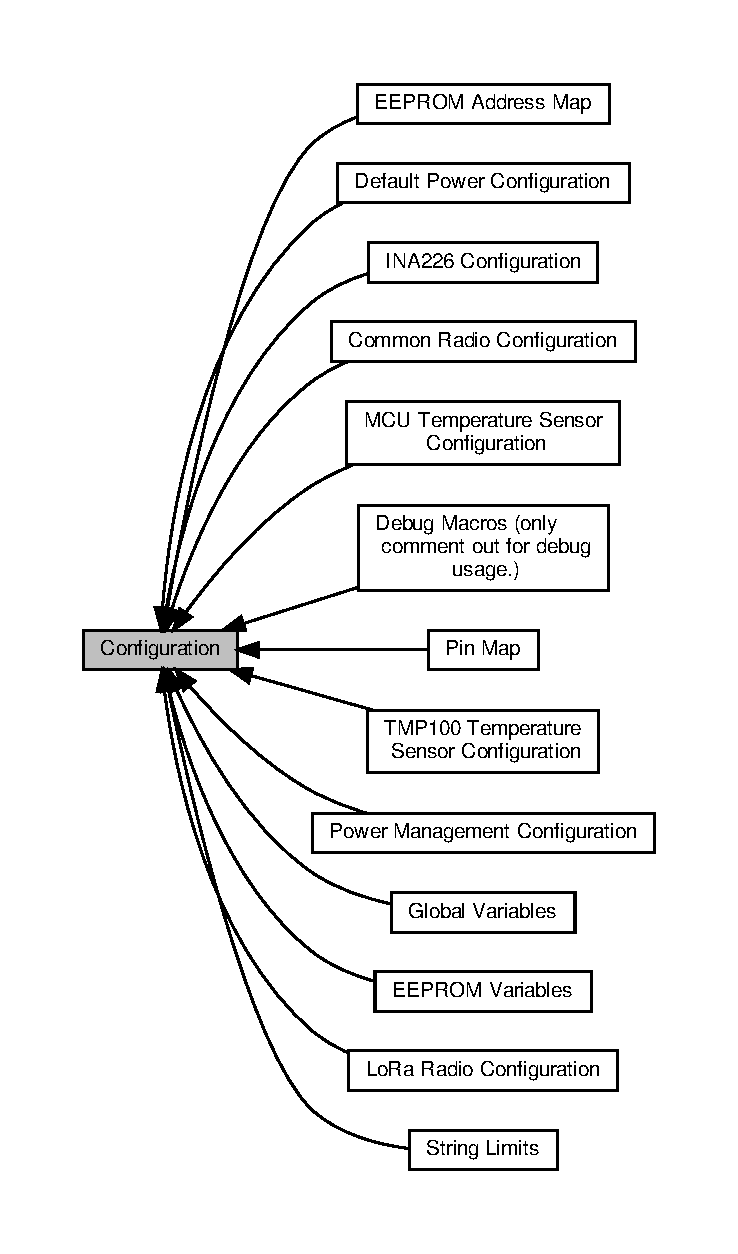
\includegraphics[height=550pt]{group__configuration__page}
\end{center}
\end{figure}
\subsection*{Modules}
\begin{DoxyCompactItemize}
\item 
\hyperlink{group__defines__string__memory__limits}{String Limits}
\item 
\hyperlink{group__defines__debug__macros}{Debug Macros (only comment out for debug usage.)}
\item 
\hyperlink{group__defines__power__management__configuration}{Power Management Configuration}
\item 
\hyperlink{group__defines__default__power__configuration}{Default Power Configuration}
\item 
\hyperlink{group__defines__ina226__configuration}{I\+N\+A226 Configuration}
\item 
\hyperlink{group__defines__eeprom__address__map}{E\+E\+P\+R\+O\+M Address Map}
\begin{DoxyCompactList}\small\item\em \tabulinesep=1mm
\begin{longtabu} spread 0pt [c]{*{4}{|X[-1]}|}
\hline
\rowcolor{\tableheadbgcolor}\textbf{ Description}&\textbf{ Start Address}&\textbf{ End Address}&\textbf{ Length (bytes)  }\\\cline{1-4}
\endfirsthead
\hline
\endfoot
\hline
\rowcolor{\tableheadbgcolor}\textbf{ Description}&\textbf{ Start Address}&\textbf{ End Address}&\textbf{ Length (bytes)  }\\\cline{1-4}
\endhead
Deployment counter (uint8\+\_\+t).&0x0000&0x0000&1 \\\cline{1-4}
Power configuration (\hyperlink{unionpower_config__t}{power\+Config\+\_\+t}).&0x0001&0x0001&1 \\\cline{1-4}
First run (uint8\+\_\+t).&0x0002&0x0002&1 \\\cline{1-4}
Restart counter (uint16\+\_\+t).&0x0003&0x0004&2 \\\cline{1-4}
F\+SK receive window length (uint8\+\_\+t).&0x0005&0x0005&1 \\\cline{1-4}
Lo\+Ra receive window length (uint8\+\_\+t).&0x0006&0x0006&1 \\\cline{1-4}
Seconds elapsed since last reset (uint32\+\_\+t).&0x0007&0x000A&4 \\\cline{1-4}
Number of main loop iterations (uint8\+\_\+t).&0x000B&0x000B&1 \\\cline{1-4}
Number of received valid Lo\+Ra frames (uint16\+\_\+t).&0x000C&0x000D&2 \\\cline{1-4}
Number of received invalid Lo\+Ra frames (uint16\+\_\+t).&0x000E&0x000F&2 \\\cline{1-4}
Number of received valid F\+SK frames (uint16\+\_\+t).&0x0010&0x0011&2 \\\cline{1-4}
Number of received invalid F\+SK frames (uint16\+\_\+t).&0x0012&0x0013&2 \\\cline{1-4}
Length of callsign (uint8\+\_\+t).&0x0014&0x0014&1 \\\cline{1-4}
Callsign (C-\/string, max M\+A\+X\+\_\+\+S\+T\+R\+I\+N\+G\+\_\+\+L\+E\+N\+G\+TH bytes).&0x00015&0x0035&M\+A\+X\+\_\+\+S\+T\+R\+I\+N\+G\+\_\+\+L\+E\+N\+G\+TH \\\cline{1-4}
Charging voltage stats (min -\/ avg -\/ max, 3x uint8\+\_\+t).&0x0040&0x0042&3 \\\cline{1-4}
Charging current stats (min -\/ avg -\/ max, 3x int16\+\_\+t).&0x0043&0x0048&6 \\\cline{1-4}
Battery voltage stats (min -\/ avg -\/ max, 3x uint8\+\_\+t).&0x0049&0x004B&3 \\\cline{1-4}
Solar cell A voltage stats (min -\/ avg -\/ max, 3x uint8\+\_\+t).&0x004C&0x004E&3 \\\cline{1-4}
Solar cell B voltage stats (min -\/ avg -\/ max, 3x uint8\+\_\+t).&0x004F&0x0051&3 \\\cline{1-4}
Solar cell C voltage stats (min -\/ avg -\/ max, 3x uint8\+\_\+t).&0x0052&0x0054&3 \\\cline{1-4}
Battery temperature stats (min -\/ avg -\/ max, 3x int16\+\_\+t).&0x0055&0x005A&6 \\\cline{1-4}
Board temperature stats (min -\/ avg -\/ max, 3x int16\+\_\+t).&0x005B&0x0060&6 \\\cline{1-4}
M\+CU temperature stats (min -\/ avg -\/ max, 3x int8\+\_\+t).&0x0061&0x0063&3 \\\cline{1-4}
Total&&&72 \\\cline{1-4}
\end{longtabu}
\end{DoxyCompactList}\item 
\hyperlink{group__defines__eeprom__variables}{E\+E\+P\+R\+O\+M Variables}
\item 
\hyperlink{group__defines__pin__map}{Pin Map}
\begin{DoxyCompactList}\small\item\em \tabulinesep=1mm
\begin{longtabu} spread 0pt [c]{*{5}{|X[-1]}|}
\hline
\rowcolor{\tableheadbgcolor}\textbf{ Description}&\textbf{ Arduino core pin}&\textbf{ Physical pin}&\textbf{ Mode}&\textbf{ Direction  }\\\cline{1-5}
\endfirsthead
\hline
\endfoot
\hline
\rowcolor{\tableheadbgcolor}\textbf{ Description}&\textbf{ Arduino core pin}&\textbf{ Physical pin}&\textbf{ Mode}&\textbf{ Direction  }\\\cline{1-5}
\endhead
Solar Cell A Voltage.&A0&P\+C0&A\+N\+A\+L\+OG&IN \\\cline{1-5}
Solar Cell B Voltage.&A7&A\+D\+C7&A\+N\+A\+L\+OG&IN \\\cline{1-5}
Solar Cell C Voltage.&A2&P\+C2&A\+N\+A\+L\+OG&IN \\\cline{1-5}
Analog source for the random number generator (should be left floating).&A6&A\+D\+C6&A\+N\+A\+L\+OG&IN \\\cline{1-5}
M\+P\+PT power control pin.&10&P\+B2&D\+I\+G\+I\+T\+AL&O\+UT \\\cline{1-5}
Deployment mosfet number 1 (controls nicrome wires).&9&P\+B2&D\+I\+G\+I\+T\+AL&O\+UT \\\cline{1-5}
Deployment mosfet number 2 (controls nicrome wires).&8&P\+B0&D\+I\+G\+I\+T\+AL&O\+UT \\\cline{1-5}
Watchdog signal pin.&4&P\+D4&D\+I\+G\+I\+T\+AL&O\+UT \\\cline{1-5}
Radio chip select.&7&P\+D7&D\+I\+G\+I\+T\+AL&O\+UT \\\cline{1-5}
Radio digital pin 1 for reading direct data.&2&P\+D2&D\+I\+G\+I\+T\+AL&IN \\\cline{1-5}
Radio B\+U\+SY pin.&6&P\+D6&D\+I\+G\+I\+T\+AL&IN \\\cline{1-5}
Radio N\+R\+ST pin.&NC&N/A&N/A&N/A \\\cline{1-5}
\end{longtabu}
\end{DoxyCompactList}\item 
\hyperlink{group__defines__tmp100__configuration}{T\+M\+P100 Temperature Sensor Configuration}
\item 
\hyperlink{group__defines__mcu__temperature__configuration}{M\+C\+U Temperature Sensor Configuration}
\item 
\hyperlink{group__defines__radio__common__configuraiton}{Common Radio Configuration}
\item 
\hyperlink{group__defines__radio__lora__configuration}{Lo\+Ra Radio Configuration}
\begin{DoxyCompactList}\small\item\em \tabulinesep=1mm
\begin{longtabu} spread 0pt [c]{*{3}{|X[-1]}|}
\hline
\rowcolor{\tableheadbgcolor}\textbf{ Description}&\textbf{ Value}&\textbf{ Units  }\\\cline{1-3}
\endfirsthead
\hline
\endfoot
\hline
\rowcolor{\tableheadbgcolor}\textbf{ Description}&\textbf{ Value}&\textbf{ Units  }\\\cline{1-3}
\endhead
Carrier Frequency.&436.\+7&M\+Hz \\\cline{1-3}
Bandwidth.&125.\+0&K\+Hz dual sideband \\\cline{1-3}
Spreading Factor.&11&N/A \\\cline{1-3}
Spreading Factor Alternate.&10&N/A \\\cline{1-3}
Coding rate.&8 (4/8 Extended Hamming)&N/A \\\cline{1-3}
Output Power.&20&d\+Bm \\\cline{1-3}
Current limit.&160.\+0&mA \\\cline{1-3}
\end{longtabu}
\end{DoxyCompactList}\item 
\hyperlink{group__defines__global__variables}{Global Variables}
\end{DoxyCompactItemize}
\subsection*{Functions}
\begin{DoxyCompactItemize}
\item 
\mbox{\Hypertarget{group__configuration__page_ga7ec89402e9818cff2cb6543057cfa82c}\label{group__configuration__page_ga7ec89402e9818cff2cb6543057cfa82c}} 
void \hyperlink{group__configuration__page_ga7ec89402e9818cff2cb6543057cfa82c}{Configuration\+\_\+\+Setup\+\_\+\+Pins} ()
\begin{DoxyCompactList}\small\item\em This function is called at the very beginning of the satellite\textquotesingle{}s startup to configure each pin. \end{DoxyCompactList}\end{DoxyCompactItemize}


\subsection{Detailed Description}

\hypertarget{group__defines__string__memory__limits}{}\section{String Limits}
\label{group__defines__string__memory__limits}\index{String Limits@{String Limits}}
Collaboration diagram for String Limits\+:
\nopagebreak
\begin{figure}[H]
\begin{center}
\leavevmode
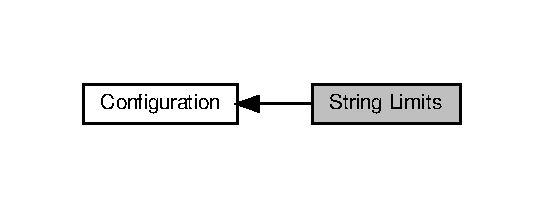
\includegraphics[width=261pt]{group__defines__string__memory__limits}
\end{center}
\end{figure}
\subsection*{Macros}
\begin{DoxyCompactItemize}
\item 
\#define \hyperlink{group__defines__string__memory__limits_ga6789ebc0df71a8ef76bfbb4fb5f74aad}{M\+A\+X\+\_\+\+S\+T\+R\+I\+N\+G\+\_\+\+L\+E\+N\+G\+TH}~32
\item 
\#define \hyperlink{group__defines__string__memory__limits_gae4e308c6dc1882b7571c0eef47e07800}{M\+A\+X\+\_\+\+O\+P\+T\+\_\+\+D\+A\+T\+A\+\_\+\+L\+E\+N\+G\+TH}~128
\item 
\#define \hyperlink{group__defines__string__memory__limits_ga03d448ca7b11d1c3e1768aebdda93af2}{M\+A\+X\+\_\+\+R\+A\+D\+I\+O\+\_\+\+B\+U\+F\+F\+E\+R\+\_\+\+L\+E\+N\+G\+TH}~(\hyperlink{group__defines__string__memory__limits_ga6789ebc0df71a8ef76bfbb4fb5f74aad}{M\+A\+X\+\_\+\+S\+T\+R\+I\+N\+G\+\_\+\+L\+E\+N\+G\+TH} + 2 + \hyperlink{group__defines__string__memory__limits_gae4e308c6dc1882b7571c0eef47e07800}{M\+A\+X\+\_\+\+O\+P\+T\+\_\+\+D\+A\+T\+A\+\_\+\+L\+E\+N\+G\+TH})
\end{DoxyCompactItemize}


\subsection{Detailed Description}


\subsection{Macro Definition Documentation}
\mbox{\Hypertarget{group__defines__string__memory__limits_gae4e308c6dc1882b7571c0eef47e07800}\label{group__defines__string__memory__limits_gae4e308c6dc1882b7571c0eef47e07800}} 
\index{String Limits@{String Limits}!M\+A\+X\+\_\+\+O\+P\+T\+\_\+\+D\+A\+T\+A\+\_\+\+L\+E\+N\+G\+TH@{M\+A\+X\+\_\+\+O\+P\+T\+\_\+\+D\+A\+T\+A\+\_\+\+L\+E\+N\+G\+TH}}
\index{M\+A\+X\+\_\+\+O\+P\+T\+\_\+\+D\+A\+T\+A\+\_\+\+L\+E\+N\+G\+TH@{M\+A\+X\+\_\+\+O\+P\+T\+\_\+\+D\+A\+T\+A\+\_\+\+L\+E\+N\+G\+TH}!String Limits@{String Limits}}
\subsubsection{\texorpdfstring{M\+A\+X\+\_\+\+O\+P\+T\+\_\+\+D\+A\+T\+A\+\_\+\+L\+E\+N\+G\+TH}{MAX\_OPT\_DATA\_LENGTH}}
{\footnotesize\ttfamily \#define M\+A\+X\+\_\+\+O\+P\+T\+\_\+\+D\+A\+T\+A\+\_\+\+L\+E\+N\+G\+TH~128}

Optional data length limit (bytes). 

Definition at line 30 of file configuration.\+h.

\mbox{\Hypertarget{group__defines__string__memory__limits_ga03d448ca7b11d1c3e1768aebdda93af2}\label{group__defines__string__memory__limits_ga03d448ca7b11d1c3e1768aebdda93af2}} 
\index{String Limits@{String Limits}!M\+A\+X\+\_\+\+R\+A\+D\+I\+O\+\_\+\+B\+U\+F\+F\+E\+R\+\_\+\+L\+E\+N\+G\+TH@{M\+A\+X\+\_\+\+R\+A\+D\+I\+O\+\_\+\+B\+U\+F\+F\+E\+R\+\_\+\+L\+E\+N\+G\+TH}}
\index{M\+A\+X\+\_\+\+R\+A\+D\+I\+O\+\_\+\+B\+U\+F\+F\+E\+R\+\_\+\+L\+E\+N\+G\+TH@{M\+A\+X\+\_\+\+R\+A\+D\+I\+O\+\_\+\+B\+U\+F\+F\+E\+R\+\_\+\+L\+E\+N\+G\+TH}!String Limits@{String Limits}}
\subsubsection{\texorpdfstring{M\+A\+X\+\_\+\+R\+A\+D\+I\+O\+\_\+\+B\+U\+F\+F\+E\+R\+\_\+\+L\+E\+N\+G\+TH}{MAX\_RADIO\_BUFFER\_LENGTH}}
{\footnotesize\ttfamily \#define M\+A\+X\+\_\+\+R\+A\+D\+I\+O\+\_\+\+B\+U\+F\+F\+E\+R\+\_\+\+L\+E\+N\+G\+TH~(\hyperlink{group__defines__string__memory__limits_ga6789ebc0df71a8ef76bfbb4fb5f74aad}{M\+A\+X\+\_\+\+S\+T\+R\+I\+N\+G\+\_\+\+L\+E\+N\+G\+TH} + 2 + \hyperlink{group__defines__string__memory__limits_gae4e308c6dc1882b7571c0eef47e07800}{M\+A\+X\+\_\+\+O\+P\+T\+\_\+\+D\+A\+T\+A\+\_\+\+L\+E\+N\+G\+TH})}

Radio buffer length limit. 

Definition at line 31 of file configuration.\+h.

\mbox{\Hypertarget{group__defines__string__memory__limits_ga6789ebc0df71a8ef76bfbb4fb5f74aad}\label{group__defines__string__memory__limits_ga6789ebc0df71a8ef76bfbb4fb5f74aad}} 
\index{String Limits@{String Limits}!M\+A\+X\+\_\+\+S\+T\+R\+I\+N\+G\+\_\+\+L\+E\+N\+G\+TH@{M\+A\+X\+\_\+\+S\+T\+R\+I\+N\+G\+\_\+\+L\+E\+N\+G\+TH}}
\index{M\+A\+X\+\_\+\+S\+T\+R\+I\+N\+G\+\_\+\+L\+E\+N\+G\+TH@{M\+A\+X\+\_\+\+S\+T\+R\+I\+N\+G\+\_\+\+L\+E\+N\+G\+TH}!String Limits@{String Limits}}
\subsubsection{\texorpdfstring{M\+A\+X\+\_\+\+S\+T\+R\+I\+N\+G\+\_\+\+L\+E\+N\+G\+TH}{MAX\_STRING\_LENGTH}}
{\footnotesize\ttfamily \#define M\+A\+X\+\_\+\+S\+T\+R\+I\+N\+G\+\_\+\+L\+E\+N\+G\+TH~32}

String length limit (bytes). 

Definition at line 29 of file configuration.\+h.


\hypertarget{group__defines__debug__macros}{}\section{Debug Macros (only comment out for debug usage.)}
\label{group__defines__debug__macros}\index{Debug Macros (only comment out for debug usage.)@{Debug Macros (only comment out for debug usage.)}}
Collaboration diagram for Debug Macros (only comment out for debug usage.)\+:
\nopagebreak
\begin{figure}[H]
\begin{center}
\leavevmode
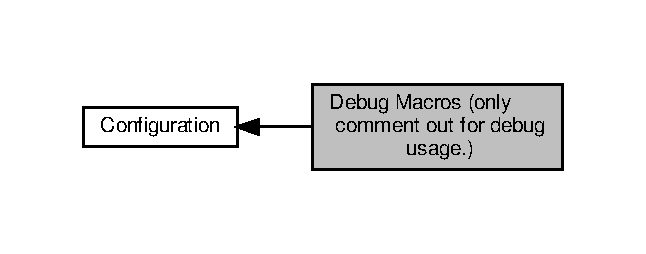
\includegraphics[width=310pt]{group__defines__debug__macros}
\end{center}
\end{figure}
\subsection*{Macros}
\begin{DoxyCompactItemize}
\item 
\#define \hyperlink{group__defines__debug__macros_ga9540d97eef375819a92593f0e9a7a1f6}{E\+N\+A\+B\+L\+E\+\_\+\+T\+R\+A\+N\+S\+M\+I\+S\+S\+I\+O\+N\+\_\+\+C\+O\+N\+T\+R\+OL}
\item 
\#define \hyperlink{group__defines__debug__macros_ga0a56ed473e6b28f5f47a91daad56691b}{E\+N\+A\+B\+L\+E\+\_\+\+D\+E\+P\+L\+O\+Y\+M\+E\+N\+T\+\_\+\+S\+E\+Q\+U\+E\+N\+CE}
\item 
\#define \hyperlink{group__defines__debug__macros_ga0fe0251d8d01ab2080467443b07af5de}{E\+N\+A\+B\+L\+E\+\_\+\+I\+N\+T\+E\+R\+V\+A\+L\+\_\+\+C\+O\+N\+T\+R\+OL}
\item 
\#define \hyperlink{group__defines__debug__macros_ga87db321802eb0b214234ee6936607fe3}{E\+N\+A\+B\+L\+E\+\_\+\+I\+N\+A226}
\end{DoxyCompactItemize}


\subsection{Detailed Description}
\begin{DoxyRefDesc}{Test}
\item[\hyperlink{test__test000016}{Test}](ID C\+O\+N\+F\+\_\+\+D\+E\+B\+U\+G\+\_\+\+M\+A\+C\+R\+O\+S\+\_\+\+T0) (S\+EV 1) Uncomment E\+N\+A\+B\+L\+E\+\_\+\+T\+R\+A\+N\+S\+M\+I\+S\+S\+I\+O\+N\+\_\+\+C\+O\+N\+T\+R\+OL, test no transmissions are produced. 

(ID C\+O\+N\+F\+\_\+\+D\+E\+B\+U\+G\+\_\+\+M\+A\+C\+R\+O\+S\+\_\+\+T1) (S\+EV 1) Uncomment E\+N\+A\+B\+L\+E\+\_\+\+D\+E\+P\+L\+O\+Y\+M\+E\+N\+T\+\_\+\+S\+E\+Q\+U\+E\+N\+CE, test no deployment sequence ran (this define is for debugging purposes). 

(ID C\+O\+N\+F\+\_\+\+D\+E\+B\+U\+G\+\_\+\+M\+A\+C\+R\+O\+S\+\_\+\+T2) (S\+EV 1) Uncomment E\+N\+A\+B\+L\+E\+\_\+\+I\+N\+T\+E\+R\+V\+A\+L\+\_\+\+C\+O\+N\+T\+R\+OL, test that the battery voltages have no affect on the sleep duration. 

(ID C\+O\+N\+F\+\_\+\+D\+E\+B\+U\+G\+\_\+\+M\+A\+C\+R\+O\+S\+\_\+\+T3) (S\+EV 1) Uncomment E\+N\+A\+B\+L\+E\+\_\+\+I\+N\+A226, test that the current readings are correct.\end{DoxyRefDesc}


\subsection{Macro Definition Documentation}
\mbox{\Hypertarget{group__defines__debug__macros_ga0a56ed473e6b28f5f47a91daad56691b}\label{group__defines__debug__macros_ga0a56ed473e6b28f5f47a91daad56691b}} 
\index{Debug Macros (only comment out for debug usage.)@{Debug Macros (only comment out for debug usage.)}!E\+N\+A\+B\+L\+E\+\_\+\+D\+E\+P\+L\+O\+Y\+M\+E\+N\+T\+\_\+\+S\+E\+Q\+U\+E\+N\+CE@{E\+N\+A\+B\+L\+E\+\_\+\+D\+E\+P\+L\+O\+Y\+M\+E\+N\+T\+\_\+\+S\+E\+Q\+U\+E\+N\+CE}}
\index{E\+N\+A\+B\+L\+E\+\_\+\+D\+E\+P\+L\+O\+Y\+M\+E\+N\+T\+\_\+\+S\+E\+Q\+U\+E\+N\+CE@{E\+N\+A\+B\+L\+E\+\_\+\+D\+E\+P\+L\+O\+Y\+M\+E\+N\+T\+\_\+\+S\+E\+Q\+U\+E\+N\+CE}!Debug Macros (only comment out for debug usage.)@{Debug Macros (only comment out for debug usage.)}}
\subsubsection{\texorpdfstring{E\+N\+A\+B\+L\+E\+\_\+\+D\+E\+P\+L\+O\+Y\+M\+E\+N\+T\+\_\+\+S\+E\+Q\+U\+E\+N\+CE}{ENABLE\_DEPLOYMENT\_SEQUENCE}}
{\footnotesize\ttfamily \#define E\+N\+A\+B\+L\+E\+\_\+\+D\+E\+P\+L\+O\+Y\+M\+E\+N\+T\+\_\+\+S\+E\+Q\+U\+E\+N\+CE}

Comment out to disable deployment sequence 

Definition at line 48 of file configuration.\+h.

\mbox{\Hypertarget{group__defines__debug__macros_ga87db321802eb0b214234ee6936607fe3}\label{group__defines__debug__macros_ga87db321802eb0b214234ee6936607fe3}} 
\index{Debug Macros (only comment out for debug usage.)@{Debug Macros (only comment out for debug usage.)}!E\+N\+A\+B\+L\+E\+\_\+\+I\+N\+A226@{E\+N\+A\+B\+L\+E\+\_\+\+I\+N\+A226}}
\index{E\+N\+A\+B\+L\+E\+\_\+\+I\+N\+A226@{E\+N\+A\+B\+L\+E\+\_\+\+I\+N\+A226}!Debug Macros (only comment out for debug usage.)@{Debug Macros (only comment out for debug usage.)}}
\subsubsection{\texorpdfstring{E\+N\+A\+B\+L\+E\+\_\+\+I\+N\+A226}{ENABLE\_INA226}}
{\footnotesize\ttfamily \#define E\+N\+A\+B\+L\+E\+\_\+\+I\+N\+A226}

Comment out to skip I\+N\+A226 reading 

Definition at line 50 of file configuration.\+h.

\mbox{\Hypertarget{group__defines__debug__macros_ga0fe0251d8d01ab2080467443b07af5de}\label{group__defines__debug__macros_ga0fe0251d8d01ab2080467443b07af5de}} 
\index{Debug Macros (only comment out for debug usage.)@{Debug Macros (only comment out for debug usage.)}!E\+N\+A\+B\+L\+E\+\_\+\+I\+N\+T\+E\+R\+V\+A\+L\+\_\+\+C\+O\+N\+T\+R\+OL@{E\+N\+A\+B\+L\+E\+\_\+\+I\+N\+T\+E\+R\+V\+A\+L\+\_\+\+C\+O\+N\+T\+R\+OL}}
\index{E\+N\+A\+B\+L\+E\+\_\+\+I\+N\+T\+E\+R\+V\+A\+L\+\_\+\+C\+O\+N\+T\+R\+OL@{E\+N\+A\+B\+L\+E\+\_\+\+I\+N\+T\+E\+R\+V\+A\+L\+\_\+\+C\+O\+N\+T\+R\+OL}!Debug Macros (only comment out for debug usage.)@{Debug Macros (only comment out for debug usage.)}}
\subsubsection{\texorpdfstring{E\+N\+A\+B\+L\+E\+\_\+\+I\+N\+T\+E\+R\+V\+A\+L\+\_\+\+C\+O\+N\+T\+R\+OL}{ENABLE\_INTERVAL\_CONTROL}}
{\footnotesize\ttfamily \#define E\+N\+A\+B\+L\+E\+\_\+\+I\+N\+T\+E\+R\+V\+A\+L\+\_\+\+C\+O\+N\+T\+R\+OL}

Comment out to disable automatic sleep interval and transmission control 

Definition at line 49 of file configuration.\+h.

\mbox{\Hypertarget{group__defines__debug__macros_ga9540d97eef375819a92593f0e9a7a1f6}\label{group__defines__debug__macros_ga9540d97eef375819a92593f0e9a7a1f6}} 
\index{Debug Macros (only comment out for debug usage.)@{Debug Macros (only comment out for debug usage.)}!E\+N\+A\+B\+L\+E\+\_\+\+T\+R\+A\+N\+S\+M\+I\+S\+S\+I\+O\+N\+\_\+\+C\+O\+N\+T\+R\+OL@{E\+N\+A\+B\+L\+E\+\_\+\+T\+R\+A\+N\+S\+M\+I\+S\+S\+I\+O\+N\+\_\+\+C\+O\+N\+T\+R\+OL}}
\index{E\+N\+A\+B\+L\+E\+\_\+\+T\+R\+A\+N\+S\+M\+I\+S\+S\+I\+O\+N\+\_\+\+C\+O\+N\+T\+R\+OL@{E\+N\+A\+B\+L\+E\+\_\+\+T\+R\+A\+N\+S\+M\+I\+S\+S\+I\+O\+N\+\_\+\+C\+O\+N\+T\+R\+OL}!Debug Macros (only comment out for debug usage.)@{Debug Macros (only comment out for debug usage.)}}
\subsubsection{\texorpdfstring{E\+N\+A\+B\+L\+E\+\_\+\+T\+R\+A\+N\+S\+M\+I\+S\+S\+I\+O\+N\+\_\+\+C\+O\+N\+T\+R\+OL}{ENABLE\_TRANSMISSION\_CONTROL}}
{\footnotesize\ttfamily \#define E\+N\+A\+B\+L\+E\+\_\+\+T\+R\+A\+N\+S\+M\+I\+S\+S\+I\+O\+N\+\_\+\+C\+O\+N\+T\+R\+OL}

Comment out to disable transmission control (transmission disable and no transmissions in low power mode) 

Definition at line 47 of file configuration.\+h.


\hypertarget{group__defines__power__management__configuration}{}\section{Power Management Configuration}
\label{group__defines__power__management__configuration}\index{Power Management Configuration@{Power Management Configuration}}
Collaboration diagram for Power Management Configuration\+:
\nopagebreak
\begin{figure}[H]
\begin{center}
\leavevmode
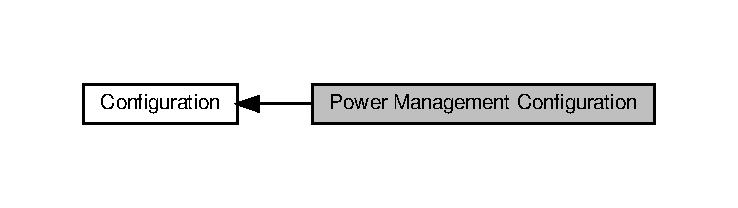
\includegraphics[width=350pt]{group__defines__power__management__configuration}
\end{center}
\end{figure}
\subsection*{Macros}
\begin{DoxyCompactItemize}
\item 
\#define \hyperlink{group__defines__power__management__configuration_gab56ff9c956d5497736a78ad136ad42ce}{B\+A\+T\+T\+E\+R\+Y\+\_\+\+V\+O\+L\+T\+A\+G\+E\+\_\+\+L\+I\+M\+IT}~3.\+8f
\item 
\#define \hyperlink{group__defines__power__management__configuration_ga49ce03eb4bd79a0060a41d793a946a83}{B\+A\+T\+T\+E\+R\+Y\+\_\+\+C\+W\+\_\+\+B\+E\+E\+P\+\_\+\+V\+O\+L\+T\+A\+G\+E\+\_\+\+L\+I\+M\+IT}~3.\+8f
\item 
\#define \hyperlink{group__defines__power__management__configuration_gac16481577dc431a739e4a370c55ac31b}{B\+A\+T\+T\+E\+R\+Y\+\_\+\+T\+E\+M\+P\+E\+R\+A\+T\+U\+R\+E\+\_\+\+L\+I\+M\+IT}~-\/0.\+7f
\item 
\#define \hyperlink{group__defines__power__management__configuration_gab197bb7848461922d4807f622f8e1fa1}{W\+A\+T\+C\+H\+D\+O\+G\+\_\+\+L\+O\+O\+P\+\_\+\+H\+E\+A\+R\+T\+B\+E\+A\+T\+\_\+\+P\+E\+R\+I\+OD}~1000
\item 
\#define \hyperlink{group__defines__power__management__configuration_ga9cc0ca1764367faad6417786f2bf6c31}{W\+A\+T\+C\+H\+D\+O\+G\+\_\+\+R\+E\+S\+E\+T\+\_\+\+N\+U\+M\+\_\+\+S\+L\+E\+E\+P\+\_\+\+C\+Y\+C\+L\+ES}~4
\item 
\#define \hyperlink{group__defines__power__management__configuration_ga81e91715a5069cfc0e8c4e8abb09c7ca}{S\+L\+E\+E\+P\+\_\+\+L\+E\+N\+G\+T\+H\+\_\+\+C\+O\+N\+S\+T\+A\+NT}~0.\+9
\item 
\#define \hyperlink{group__defines__power__management__configuration_ga5570f576c017a9d49eb716091e3e6831}{D\+E\+P\+L\+O\+Y\+M\+E\+N\+T\+\_\+\+A\+T\+T\+E\+M\+P\+TS}~4
\item 
\#define \hyperlink{group__defines__power__management__configuration_ga3f2ab6a21f83ae3f1af1c47852c31873}{D\+E\+P\+L\+O\+Y\+M\+E\+N\+T\+\_\+\+S\+L\+E\+E\+P\+\_\+\+L\+E\+N\+G\+TH}~1800000
\item 
\#define \hyperlink{group__defines__power__management__configuration_gab47513da7a20ecfdd6fecd60fcdba7b0}{D\+E\+P\+L\+O\+Y\+M\+E\+N\+T\+\_\+\+D\+E\+B\+U\+G\+\_\+\+L\+E\+N\+G\+TH}~60
\item 
\#define \hyperlink{group__defines__power__management__configuration_ga19207306df03c631116fc3f6edbd0295}{D\+E\+P\+L\+O\+Y\+M\+E\+N\+T\+\_\+\+D\+E\+B\+U\+G\+\_\+\+S\+A\+M\+P\+L\+E\+\_\+\+P\+E\+R\+I\+OD}~1000
\item 
\#define \hyperlink{group__defines__power__management__configuration_gaa44a203cdf6536532202678823a18542}{A\+U\+T\+O\+D\+E\+P\+L\+O\+Y\+\_\+\+D\+E\+L\+AY}~1200
\end{DoxyCompactItemize}


\subsection{Detailed Description}
\begin{DoxyRefDesc}{Test}
\item[\hyperlink{test__test000017}{Test}](ID C\+O\+N\+F\+\_\+\+P\+O\+W\+E\+R\+\_\+\+M\+A\+N\+A\+G\+E\+M\+E\+N\+T\+\_\+\+T0) (S\+EV 1) Check that the satellite switches to low power mode when its voltage goes below B\+A\+T\+T\+E\+R\+Y\+\_\+\+V\+O\+L\+T\+A\+G\+E\+\_\+\+L\+I\+M\+IT. 

(ID C\+O\+N\+F\+\_\+\+P\+O\+W\+E\+R\+\_\+\+M\+A\+N\+A\+G\+E\+M\+E\+N\+T\+\_\+\+T1) (S\+EV 2) Check that the satellite sends a morse beacon transmission when it switches to Low Power Mode. 

(ID C\+O\+N\+F\+\_\+\+P\+O\+W\+E\+R\+\_\+\+M\+A\+N\+A\+G\+E\+M\+E\+N\+T\+\_\+\+T2) (S\+EV 1) Check that the battery stops charging when the temperature goes below this threshold, and starts charging again when it is not. 

(ID C\+O\+N\+F\+\_\+\+P\+O\+W\+E\+R\+\_\+\+M\+A\+N\+A\+G\+E\+M\+E\+N\+T\+\_\+\+T3) (S\+EV 1) Check that the watchdog is signalled every W\+A\+T\+C\+H\+D\+O\+G\+\_\+\+L\+O\+O\+P\+\_\+\+H\+E\+A\+R\+T\+B\+E\+A\+T\+\_\+\+P\+E\+R\+I\+OD. 

(ID C\+O\+N\+F\+\_\+\+P\+O\+W\+E\+R\+\_\+\+M\+A\+N\+A\+G\+E\+M\+E\+N\+T\+\_\+\+T4) (S\+EV 1) Check that the satellite sleeping times using the S\+L\+E\+E\+P\+\_\+\+L\+E\+N\+G\+T\+H\+\_\+\+C\+O\+N\+S\+T\+A\+NT is suitable to account for the Low\+Power libraries overhead. 

(ID C\+O\+N\+F\+\_\+\+P\+O\+W\+E\+R\+\_\+\+M\+A\+N\+A\+G\+E\+M\+E\+N\+T\+\_\+\+T5) (S\+EV 1) Check that the satellite does not deploy after D\+E\+P\+L\+O\+Y\+M\+E\+N\+T\+\_\+\+A\+T\+T\+E\+M\+PS has reached. 

(ID C\+O\+N\+F\+\_\+\+P\+O\+W\+E\+R\+\_\+\+M\+A\+N\+A\+G\+E\+M\+E\+N\+T\+\_\+\+T6) (S\+EV 1) Check that the satellite waits for this amount of time before the deploy sequence starts, this is for jettison. 

(ID C\+O\+N\+F\+\_\+\+P\+O\+W\+E\+R\+\_\+\+M\+A\+N\+A\+G\+E\+M\+E\+N\+T\+\_\+\+T7) (S\+EV 5) Check that each debug print waits D\+E\+P\+L\+O\+Y\+M\+E\+N\+T\+\_\+\+D\+E\+B\+U\+G\+\_\+\+S\+A\+M\+P\+L\+E\+\_\+\+P\+E\+R\+I\+OD amount of time between each print.\end{DoxyRefDesc}


\begin{DoxyRefDesc}{Todo}
\item[\hyperlink{todo__todo000001}{Todo}]Julian -\/$>$ Set appropriate B\+A\+T\+T\+E\+R\+Y\+\_\+\+V\+O\+L\+T\+A\+G\+E\+\_\+\+L\+I\+M\+IT and B\+A\+T\+T\+E\+R\+Y\+\_\+\+C\+W\+\_\+\+B\+E\+E\+P\+\_\+\+V\+O\+L\+T\+A\+G\+E\+\_\+\+L\+I\+M\+IT\end{DoxyRefDesc}


\subsection{Macro Definition Documentation}
\mbox{\Hypertarget{group__defines__power__management__configuration_gaa44a203cdf6536532202678823a18542}\label{group__defines__power__management__configuration_gaa44a203cdf6536532202678823a18542}} 
\index{Power Management Configuration@{Power Management Configuration}!A\+U\+T\+O\+D\+E\+P\+L\+O\+Y\+\_\+\+D\+E\+L\+AY@{A\+U\+T\+O\+D\+E\+P\+L\+O\+Y\+\_\+\+D\+E\+L\+AY}}
\index{A\+U\+T\+O\+D\+E\+P\+L\+O\+Y\+\_\+\+D\+E\+L\+AY@{A\+U\+T\+O\+D\+E\+P\+L\+O\+Y\+\_\+\+D\+E\+L\+AY}!Power Management Configuration@{Power Management Configuration}}
\subsubsection{\texorpdfstring{A\+U\+T\+O\+D\+E\+P\+L\+O\+Y\+\_\+\+D\+E\+L\+AY}{AUTODEPLOY\_DELAY}}
{\footnotesize\ttfamily \#define A\+U\+T\+O\+D\+E\+P\+L\+O\+Y\+\_\+\+D\+E\+L\+AY~1200}

How long to wait bevore attempting automated deployment in main loop (seconds). See\+: Fossa\+Sat1\+B.\+ino 

Definition at line 82 of file configuration.\+h.

\mbox{\Hypertarget{group__defines__power__management__configuration_ga49ce03eb4bd79a0060a41d793a946a83}\label{group__defines__power__management__configuration_ga49ce03eb4bd79a0060a41d793a946a83}} 
\index{Power Management Configuration@{Power Management Configuration}!B\+A\+T\+T\+E\+R\+Y\+\_\+\+C\+W\+\_\+\+B\+E\+E\+P\+\_\+\+V\+O\+L\+T\+A\+G\+E\+\_\+\+L\+I\+M\+IT@{B\+A\+T\+T\+E\+R\+Y\+\_\+\+C\+W\+\_\+\+B\+E\+E\+P\+\_\+\+V\+O\+L\+T\+A\+G\+E\+\_\+\+L\+I\+M\+IT}}
\index{B\+A\+T\+T\+E\+R\+Y\+\_\+\+C\+W\+\_\+\+B\+E\+E\+P\+\_\+\+V\+O\+L\+T\+A\+G\+E\+\_\+\+L\+I\+M\+IT@{B\+A\+T\+T\+E\+R\+Y\+\_\+\+C\+W\+\_\+\+B\+E\+E\+P\+\_\+\+V\+O\+L\+T\+A\+G\+E\+\_\+\+L\+I\+M\+IT}!Power Management Configuration@{Power Management Configuration}}
\subsubsection{\texorpdfstring{B\+A\+T\+T\+E\+R\+Y\+\_\+\+C\+W\+\_\+\+B\+E\+E\+P\+\_\+\+V\+O\+L\+T\+A\+G\+E\+\_\+\+L\+I\+M\+IT}{BATTERY\_CW\_BEEP\_VOLTAGE\_LIMIT}}
{\footnotesize\ttfamily \#define B\+A\+T\+T\+E\+R\+Y\+\_\+\+C\+W\+\_\+\+B\+E\+E\+P\+\_\+\+V\+O\+L\+T\+A\+G\+E\+\_\+\+L\+I\+M\+IT~3.\+8f}

Battery voltage limit to switch into morse beep (V). 

Definition at line 73 of file configuration.\+h.

\mbox{\Hypertarget{group__defines__power__management__configuration_gac16481577dc431a739e4a370c55ac31b}\label{group__defines__power__management__configuration_gac16481577dc431a739e4a370c55ac31b}} 
\index{Power Management Configuration@{Power Management Configuration}!B\+A\+T\+T\+E\+R\+Y\+\_\+\+T\+E\+M\+P\+E\+R\+A\+T\+U\+R\+E\+\_\+\+L\+I\+M\+IT@{B\+A\+T\+T\+E\+R\+Y\+\_\+\+T\+E\+M\+P\+E\+R\+A\+T\+U\+R\+E\+\_\+\+L\+I\+M\+IT}}
\index{B\+A\+T\+T\+E\+R\+Y\+\_\+\+T\+E\+M\+P\+E\+R\+A\+T\+U\+R\+E\+\_\+\+L\+I\+M\+IT@{B\+A\+T\+T\+E\+R\+Y\+\_\+\+T\+E\+M\+P\+E\+R\+A\+T\+U\+R\+E\+\_\+\+L\+I\+M\+IT}!Power Management Configuration@{Power Management Configuration}}
\subsubsection{\texorpdfstring{B\+A\+T\+T\+E\+R\+Y\+\_\+\+T\+E\+M\+P\+E\+R\+A\+T\+U\+R\+E\+\_\+\+L\+I\+M\+IT}{BATTERY\_TEMPERATURE\_LIMIT}}
{\footnotesize\ttfamily \#define B\+A\+T\+T\+E\+R\+Y\+\_\+\+T\+E\+M\+P\+E\+R\+A\+T\+U\+R\+E\+\_\+\+L\+I\+M\+IT~-\/0.\+7f}

Battery charging temperature limit (deg. C). 

Definition at line 74 of file configuration.\+h.

\mbox{\Hypertarget{group__defines__power__management__configuration_gab56ff9c956d5497736a78ad136ad42ce}\label{group__defines__power__management__configuration_gab56ff9c956d5497736a78ad136ad42ce}} 
\index{Power Management Configuration@{Power Management Configuration}!B\+A\+T\+T\+E\+R\+Y\+\_\+\+V\+O\+L\+T\+A\+G\+E\+\_\+\+L\+I\+M\+IT@{B\+A\+T\+T\+E\+R\+Y\+\_\+\+V\+O\+L\+T\+A\+G\+E\+\_\+\+L\+I\+M\+IT}}
\index{B\+A\+T\+T\+E\+R\+Y\+\_\+\+V\+O\+L\+T\+A\+G\+E\+\_\+\+L\+I\+M\+IT@{B\+A\+T\+T\+E\+R\+Y\+\_\+\+V\+O\+L\+T\+A\+G\+E\+\_\+\+L\+I\+M\+IT}!Power Management Configuration@{Power Management Configuration}}
\subsubsection{\texorpdfstring{B\+A\+T\+T\+E\+R\+Y\+\_\+\+V\+O\+L\+T\+A\+G\+E\+\_\+\+L\+I\+M\+IT}{BATTERY\_VOLTAGE\_LIMIT}}
{\footnotesize\ttfamily \#define B\+A\+T\+T\+E\+R\+Y\+\_\+\+V\+O\+L\+T\+A\+G\+E\+\_\+\+L\+I\+M\+IT~3.\+8f}

Battery voltage limit to enable low power mode (V). 

Definition at line 72 of file configuration.\+h.

\mbox{\Hypertarget{group__defines__power__management__configuration_ga5570f576c017a9d49eb716091e3e6831}\label{group__defines__power__management__configuration_ga5570f576c017a9d49eb716091e3e6831}} 
\index{Power Management Configuration@{Power Management Configuration}!D\+E\+P\+L\+O\+Y\+M\+E\+N\+T\+\_\+\+A\+T\+T\+E\+M\+P\+TS@{D\+E\+P\+L\+O\+Y\+M\+E\+N\+T\+\_\+\+A\+T\+T\+E\+M\+P\+TS}}
\index{D\+E\+P\+L\+O\+Y\+M\+E\+N\+T\+\_\+\+A\+T\+T\+E\+M\+P\+TS@{D\+E\+P\+L\+O\+Y\+M\+E\+N\+T\+\_\+\+A\+T\+T\+E\+M\+P\+TS}!Power Management Configuration@{Power Management Configuration}}
\subsubsection{\texorpdfstring{D\+E\+P\+L\+O\+Y\+M\+E\+N\+T\+\_\+\+A\+T\+T\+E\+M\+P\+TS}{DEPLOYMENT\_ATTEMPTS}}
{\footnotesize\ttfamily \#define D\+E\+P\+L\+O\+Y\+M\+E\+N\+T\+\_\+\+A\+T\+T\+E\+M\+P\+TS~4}

Number of deployment attempts. 

Definition at line 78 of file configuration.\+h.

\mbox{\Hypertarget{group__defines__power__management__configuration_gab47513da7a20ecfdd6fecd60fcdba7b0}\label{group__defines__power__management__configuration_gab47513da7a20ecfdd6fecd60fcdba7b0}} 
\index{Power Management Configuration@{Power Management Configuration}!D\+E\+P\+L\+O\+Y\+M\+E\+N\+T\+\_\+\+D\+E\+B\+U\+G\+\_\+\+L\+E\+N\+G\+TH@{D\+E\+P\+L\+O\+Y\+M\+E\+N\+T\+\_\+\+D\+E\+B\+U\+G\+\_\+\+L\+E\+N\+G\+TH}}
\index{D\+E\+P\+L\+O\+Y\+M\+E\+N\+T\+\_\+\+D\+E\+B\+U\+G\+\_\+\+L\+E\+N\+G\+TH@{D\+E\+P\+L\+O\+Y\+M\+E\+N\+T\+\_\+\+D\+E\+B\+U\+G\+\_\+\+L\+E\+N\+G\+TH}!Power Management Configuration@{Power Management Configuration}}
\subsubsection{\texorpdfstring{D\+E\+P\+L\+O\+Y\+M\+E\+N\+T\+\_\+\+D\+E\+B\+U\+G\+\_\+\+L\+E\+N\+G\+TH}{DEPLOYMENT\_DEBUG\_LENGTH}}
{\footnotesize\ttfamily \#define D\+E\+P\+L\+O\+Y\+M\+E\+N\+T\+\_\+\+D\+E\+B\+U\+G\+\_\+\+L\+E\+N\+G\+TH~60}

How long to wait until the debugging print routine breaks (s). See\+: Fossa\+Sat1\+B.\+ino 

Definition at line 80 of file configuration.\+h.

\mbox{\Hypertarget{group__defines__power__management__configuration_ga19207306df03c631116fc3f6edbd0295}\label{group__defines__power__management__configuration_ga19207306df03c631116fc3f6edbd0295}} 
\index{Power Management Configuration@{Power Management Configuration}!D\+E\+P\+L\+O\+Y\+M\+E\+N\+T\+\_\+\+D\+E\+B\+U\+G\+\_\+\+S\+A\+M\+P\+L\+E\+\_\+\+P\+E\+R\+I\+OD@{D\+E\+P\+L\+O\+Y\+M\+E\+N\+T\+\_\+\+D\+E\+B\+U\+G\+\_\+\+S\+A\+M\+P\+L\+E\+\_\+\+P\+E\+R\+I\+OD}}
\index{D\+E\+P\+L\+O\+Y\+M\+E\+N\+T\+\_\+\+D\+E\+B\+U\+G\+\_\+\+S\+A\+M\+P\+L\+E\+\_\+\+P\+E\+R\+I\+OD@{D\+E\+P\+L\+O\+Y\+M\+E\+N\+T\+\_\+\+D\+E\+B\+U\+G\+\_\+\+S\+A\+M\+P\+L\+E\+\_\+\+P\+E\+R\+I\+OD}!Power Management Configuration@{Power Management Configuration}}
\subsubsection{\texorpdfstring{D\+E\+P\+L\+O\+Y\+M\+E\+N\+T\+\_\+\+D\+E\+B\+U\+G\+\_\+\+S\+A\+M\+P\+L\+E\+\_\+\+P\+E\+R\+I\+OD}{DEPLOYMENT\_DEBUG\_SAMPLE\_PERIOD}}
{\footnotesize\ttfamily \#define D\+E\+P\+L\+O\+Y\+M\+E\+N\+T\+\_\+\+D\+E\+B\+U\+G\+\_\+\+S\+A\+M\+P\+L\+E\+\_\+\+P\+E\+R\+I\+OD~1000}

How long to wait between each debug parameter print (ms). See\+: Fossa\+Sat1\+B.\+ino 

Definition at line 81 of file configuration.\+h.

\mbox{\Hypertarget{group__defines__power__management__configuration_ga3f2ab6a21f83ae3f1af1c47852c31873}\label{group__defines__power__management__configuration_ga3f2ab6a21f83ae3f1af1c47852c31873}} 
\index{Power Management Configuration@{Power Management Configuration}!D\+E\+P\+L\+O\+Y\+M\+E\+N\+T\+\_\+\+S\+L\+E\+E\+P\+\_\+\+L\+E\+N\+G\+TH@{D\+E\+P\+L\+O\+Y\+M\+E\+N\+T\+\_\+\+S\+L\+E\+E\+P\+\_\+\+L\+E\+N\+G\+TH}}
\index{D\+E\+P\+L\+O\+Y\+M\+E\+N\+T\+\_\+\+S\+L\+E\+E\+P\+\_\+\+L\+E\+N\+G\+TH@{D\+E\+P\+L\+O\+Y\+M\+E\+N\+T\+\_\+\+S\+L\+E\+E\+P\+\_\+\+L\+E\+N\+G\+TH}!Power Management Configuration@{Power Management Configuration}}
\subsubsection{\texorpdfstring{D\+E\+P\+L\+O\+Y\+M\+E\+N\+T\+\_\+\+S\+L\+E\+E\+P\+\_\+\+L\+E\+N\+G\+TH}{DEPLOYMENT\_SLEEP\_LENGTH}}
{\footnotesize\ttfamily \#define D\+E\+P\+L\+O\+Y\+M\+E\+N\+T\+\_\+\+S\+L\+E\+E\+P\+\_\+\+L\+E\+N\+G\+TH~1800000}

Sleep for this period of time before deployment (ms) 

Definition at line 79 of file configuration.\+h.

\mbox{\Hypertarget{group__defines__power__management__configuration_ga81e91715a5069cfc0e8c4e8abb09c7ca}\label{group__defines__power__management__configuration_ga81e91715a5069cfc0e8c4e8abb09c7ca}} 
\index{Power Management Configuration@{Power Management Configuration}!S\+L\+E\+E\+P\+\_\+\+L\+E\+N\+G\+T\+H\+\_\+\+C\+O\+N\+S\+T\+A\+NT@{S\+L\+E\+E\+P\+\_\+\+L\+E\+N\+G\+T\+H\+\_\+\+C\+O\+N\+S\+T\+A\+NT}}
\index{S\+L\+E\+E\+P\+\_\+\+L\+E\+N\+G\+T\+H\+\_\+\+C\+O\+N\+S\+T\+A\+NT@{S\+L\+E\+E\+P\+\_\+\+L\+E\+N\+G\+T\+H\+\_\+\+C\+O\+N\+S\+T\+A\+NT}!Power Management Configuration@{Power Management Configuration}}
\subsubsection{\texorpdfstring{S\+L\+E\+E\+P\+\_\+\+L\+E\+N\+G\+T\+H\+\_\+\+C\+O\+N\+S\+T\+A\+NT}{SLEEP\_LENGTH\_CONSTANT}}
{\footnotesize\ttfamily \#define S\+L\+E\+E\+P\+\_\+\+L\+E\+N\+G\+T\+H\+\_\+\+C\+O\+N\+S\+T\+A\+NT~0.\+9}

Sleep times are multiplied by this constant to compensate for the Low\+Power libraries overhead. 

Definition at line 77 of file configuration.\+h.

\mbox{\Hypertarget{group__defines__power__management__configuration_gab197bb7848461922d4807f622f8e1fa1}\label{group__defines__power__management__configuration_gab197bb7848461922d4807f622f8e1fa1}} 
\index{Power Management Configuration@{Power Management Configuration}!W\+A\+T\+C\+H\+D\+O\+G\+\_\+\+L\+O\+O\+P\+\_\+\+H\+E\+A\+R\+T\+B\+E\+A\+T\+\_\+\+P\+E\+R\+I\+OD@{W\+A\+T\+C\+H\+D\+O\+G\+\_\+\+L\+O\+O\+P\+\_\+\+H\+E\+A\+R\+T\+B\+E\+A\+T\+\_\+\+P\+E\+R\+I\+OD}}
\index{W\+A\+T\+C\+H\+D\+O\+G\+\_\+\+L\+O\+O\+P\+\_\+\+H\+E\+A\+R\+T\+B\+E\+A\+T\+\_\+\+P\+E\+R\+I\+OD@{W\+A\+T\+C\+H\+D\+O\+G\+\_\+\+L\+O\+O\+P\+\_\+\+H\+E\+A\+R\+T\+B\+E\+A\+T\+\_\+\+P\+E\+R\+I\+OD}!Power Management Configuration@{Power Management Configuration}}
\subsubsection{\texorpdfstring{W\+A\+T\+C\+H\+D\+O\+G\+\_\+\+L\+O\+O\+P\+\_\+\+H\+E\+A\+R\+T\+B\+E\+A\+T\+\_\+\+P\+E\+R\+I\+OD}{WATCHDOG\_LOOP\_HEARTBEAT\_PERIOD}}
{\footnotesize\ttfamily \#define W\+A\+T\+C\+H\+D\+O\+G\+\_\+\+L\+O\+O\+P\+\_\+\+H\+E\+A\+R\+T\+B\+E\+A\+T\+\_\+\+P\+E\+R\+I\+OD~1000}

Watchdog heartbeat period in loop() (ms). 

Definition at line 75 of file configuration.\+h.

\mbox{\Hypertarget{group__defines__power__management__configuration_ga9cc0ca1764367faad6417786f2bf6c31}\label{group__defines__power__management__configuration_ga9cc0ca1764367faad6417786f2bf6c31}} 
\index{Power Management Configuration@{Power Management Configuration}!W\+A\+T\+C\+H\+D\+O\+G\+\_\+\+R\+E\+S\+E\+T\+\_\+\+N\+U\+M\+\_\+\+S\+L\+E\+E\+P\+\_\+\+C\+Y\+C\+L\+ES@{W\+A\+T\+C\+H\+D\+O\+G\+\_\+\+R\+E\+S\+E\+T\+\_\+\+N\+U\+M\+\_\+\+S\+L\+E\+E\+P\+\_\+\+C\+Y\+C\+L\+ES}}
\index{W\+A\+T\+C\+H\+D\+O\+G\+\_\+\+R\+E\+S\+E\+T\+\_\+\+N\+U\+M\+\_\+\+S\+L\+E\+E\+P\+\_\+\+C\+Y\+C\+L\+ES@{W\+A\+T\+C\+H\+D\+O\+G\+\_\+\+R\+E\+S\+E\+T\+\_\+\+N\+U\+M\+\_\+\+S\+L\+E\+E\+P\+\_\+\+C\+Y\+C\+L\+ES}!Power Management Configuration@{Power Management Configuration}}
\subsubsection{\texorpdfstring{W\+A\+T\+C\+H\+D\+O\+G\+\_\+\+R\+E\+S\+E\+T\+\_\+\+N\+U\+M\+\_\+\+S\+L\+E\+E\+P\+\_\+\+C\+Y\+C\+L\+ES}{WATCHDOG\_RESET\_NUM\_SLEEP\_CYCLES}}
{\footnotesize\ttfamily \#define W\+A\+T\+C\+H\+D\+O\+G\+\_\+\+R\+E\+S\+E\+T\+\_\+\+N\+U\+M\+\_\+\+S\+L\+E\+E\+P\+\_\+\+C\+Y\+C\+L\+ES~4}

Number of 8-\/second sleep cycles to reset watchdog 

Definition at line 76 of file configuration.\+h.


\hypertarget{group__defines__default__power__configuration}{}\section{Default Power Configuration}
\label{group__defines__default__power__configuration}\index{Default Power Configuration@{Default Power Configuration}}
Collaboration diagram for Default Power Configuration\+:
\nopagebreak
\begin{figure}[H]
\begin{center}
\leavevmode
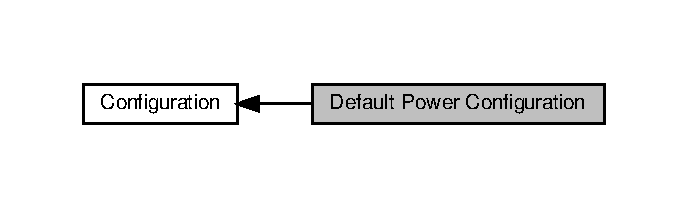
\includegraphics[width=330pt]{group__defines__default__power__configuration}
\end{center}
\end{figure}
\subsection*{Macros}
\begin{DoxyCompactItemize}
\item 
\#define \hyperlink{group__defines__default__power__configuration_gad0d7265d491052179cfbffc68a891cc6}{L\+O\+W\+\_\+\+P\+O\+W\+E\+R\+\_\+\+M\+O\+D\+E\+\_\+\+A\+C\+T\+I\+VE}~0
\item 
\#define \hyperlink{group__defines__default__power__configuration_ga7ce14dbd42484c75f63fb7557f9d133a}{L\+O\+W\+\_\+\+P\+O\+W\+E\+R\+\_\+\+M\+O\+D\+E\+\_\+\+E\+N\+A\+B\+L\+ED}~1
\item 
\#define \hyperlink{group__defines__default__power__configuration_gac1bce12d866de62b4b9eadcf81f8acb8}{M\+P\+P\+T\+\_\+\+T\+E\+M\+P\+\_\+\+S\+W\+I\+T\+C\+H\+\_\+\+E\+N\+A\+B\+L\+ED}~1
\item 
\#define \hyperlink{group__defines__default__power__configuration_ga06ae8011cff9fec1f6b3720b99f55f62}{M\+P\+P\+T\+\_\+\+K\+E\+E\+P\+\_\+\+A\+L\+I\+V\+E\+\_\+\+E\+N\+A\+B\+L\+ED}~0
\item 
\#define \hyperlink{group__defines__default__power__configuration_ga46d61f94fe26dcb9192435b6c8eaf29d}{T\+R\+A\+N\+S\+M\+I\+T\+\_\+\+E\+N\+A\+B\+L\+ED}~1
\end{DoxyCompactItemize}


\subsection{Detailed Description}
\begin{DoxyRefDesc}{Test}
\item[\hyperlink{test__test000018}{Test}](ID C\+O\+N\+F\+\_\+\+P\+O\+W\+E\+R\+\_\+\+C\+O\+N\+F\+\_\+\+T0) (S\+EV 1) Check that the low power mode works. 

(ID C\+O\+N\+F\+\_\+\+P\+O\+W\+E\+R\+\_\+\+C\+O\+N\+F\+\_\+\+T1) (S\+EV 1) Check that the low power mode can be disabled using L\+O\+W\+\_\+\+P\+O\+W\+E\+R\+\_\+\+M\+O\+D\+E\+\_\+\+E\+N\+A\+B\+L\+ED. 

(ID C\+O\+N\+F\+\_\+\+P\+O\+W\+E\+R\+\_\+\+C\+O\+N\+F\+\_\+\+T3) (S\+EV 1) Check that the M\+P\+PT is controlled by the temperature using M\+P\+P\+T\+\_\+\+T\+E\+M\+P\+\_\+\+S\+W\+I\+T\+C\+H\+\_\+\+E\+N\+A\+B\+L\+ED. 

(ID C\+O\+N\+F\+\_\+\+P\+O\+W\+E\+R\+\_\+\+C\+O\+N\+F\+\_\+\+T4) (S\+EV 1) Check that the M\+P\+PT\textquotesingle{}s temperature controller can be disabled and enabled using M\+P\+P\+T\+\_\+\+K\+E\+E\+P\+\_\+\+A\+L\+I\+V\+E\+\_\+\+E\+N\+A\+B\+L\+ED. 

(ID C\+O\+N\+F\+\_\+\+P\+O\+W\+E\+R\+\_\+\+C\+O\+N\+F\+\_\+\+T5) (S\+EV 1) Check that the satellite\textquotesingle{}s transmissions can be disabled and enabled using T\+R\+A\+N\+S\+M\+I\+T\+\_\+\+E\+N\+A\+B\+L\+ED.\end{DoxyRefDesc}


\subsection{Macro Definition Documentation}
\mbox{\Hypertarget{group__defines__default__power__configuration_gad0d7265d491052179cfbffc68a891cc6}\label{group__defines__default__power__configuration_gad0d7265d491052179cfbffc68a891cc6}} 
\index{Default Power Configuration@{Default Power Configuration}!L\+O\+W\+\_\+\+P\+O\+W\+E\+R\+\_\+\+M\+O\+D\+E\+\_\+\+A\+C\+T\+I\+VE@{L\+O\+W\+\_\+\+P\+O\+W\+E\+R\+\_\+\+M\+O\+D\+E\+\_\+\+A\+C\+T\+I\+VE}}
\index{L\+O\+W\+\_\+\+P\+O\+W\+E\+R\+\_\+\+M\+O\+D\+E\+\_\+\+A\+C\+T\+I\+VE@{L\+O\+W\+\_\+\+P\+O\+W\+E\+R\+\_\+\+M\+O\+D\+E\+\_\+\+A\+C\+T\+I\+VE}!Default Power Configuration@{Default Power Configuration}}
\subsubsection{\texorpdfstring{L\+O\+W\+\_\+\+P\+O\+W\+E\+R\+\_\+\+M\+O\+D\+E\+\_\+\+A\+C\+T\+I\+VE}{LOW\_POWER\_MODE\_ACTIVE}}
{\footnotesize\ttfamily \#define L\+O\+W\+\_\+\+P\+O\+W\+E\+R\+\_\+\+M\+O\+D\+E\+\_\+\+A\+C\+T\+I\+VE~0}

Whether the low power mode is currently active (0 is no, 1 is yes). 

Definition at line 98 of file configuration.\+h.

\mbox{\Hypertarget{group__defines__default__power__configuration_ga7ce14dbd42484c75f63fb7557f9d133a}\label{group__defines__default__power__configuration_ga7ce14dbd42484c75f63fb7557f9d133a}} 
\index{Default Power Configuration@{Default Power Configuration}!L\+O\+W\+\_\+\+P\+O\+W\+E\+R\+\_\+\+M\+O\+D\+E\+\_\+\+E\+N\+A\+B\+L\+ED@{L\+O\+W\+\_\+\+P\+O\+W\+E\+R\+\_\+\+M\+O\+D\+E\+\_\+\+E\+N\+A\+B\+L\+ED}}
\index{L\+O\+W\+\_\+\+P\+O\+W\+E\+R\+\_\+\+M\+O\+D\+E\+\_\+\+E\+N\+A\+B\+L\+ED@{L\+O\+W\+\_\+\+P\+O\+W\+E\+R\+\_\+\+M\+O\+D\+E\+\_\+\+E\+N\+A\+B\+L\+ED}!Default Power Configuration@{Default Power Configuration}}
\subsubsection{\texorpdfstring{L\+O\+W\+\_\+\+P\+O\+W\+E\+R\+\_\+\+M\+O\+D\+E\+\_\+\+E\+N\+A\+B\+L\+ED}{LOW\_POWER\_MODE\_ENABLED}}
{\footnotesize\ttfamily \#define L\+O\+W\+\_\+\+P\+O\+W\+E\+R\+\_\+\+M\+O\+D\+E\+\_\+\+E\+N\+A\+B\+L\+ED~1}

Whether the low power mode can be active (0 is no, 1 is yes). 

Definition at line 99 of file configuration.\+h.

\mbox{\Hypertarget{group__defines__default__power__configuration_ga06ae8011cff9fec1f6b3720b99f55f62}\label{group__defines__default__power__configuration_ga06ae8011cff9fec1f6b3720b99f55f62}} 
\index{Default Power Configuration@{Default Power Configuration}!M\+P\+P\+T\+\_\+\+K\+E\+E\+P\+\_\+\+A\+L\+I\+V\+E\+\_\+\+E\+N\+A\+B\+L\+ED@{M\+P\+P\+T\+\_\+\+K\+E\+E\+P\+\_\+\+A\+L\+I\+V\+E\+\_\+\+E\+N\+A\+B\+L\+ED}}
\index{M\+P\+P\+T\+\_\+\+K\+E\+E\+P\+\_\+\+A\+L\+I\+V\+E\+\_\+\+E\+N\+A\+B\+L\+ED@{M\+P\+P\+T\+\_\+\+K\+E\+E\+P\+\_\+\+A\+L\+I\+V\+E\+\_\+\+E\+N\+A\+B\+L\+ED}!Default Power Configuration@{Default Power Configuration}}
\subsubsection{\texorpdfstring{M\+P\+P\+T\+\_\+\+K\+E\+E\+P\+\_\+\+A\+L\+I\+V\+E\+\_\+\+E\+N\+A\+B\+L\+ED}{MPPT\_KEEP\_ALIVE\_ENABLED}}
{\footnotesize\ttfamily \#define M\+P\+P\+T\+\_\+\+K\+E\+E\+P\+\_\+\+A\+L\+I\+V\+E\+\_\+\+E\+N\+A\+B\+L\+ED~0}

Whether the M\+P\+PT circuit disabling feature is enabled (0 is no, 1 is yes). 

Definition at line 101 of file configuration.\+h.

\mbox{\Hypertarget{group__defines__default__power__configuration_gac1bce12d866de62b4b9eadcf81f8acb8}\label{group__defines__default__power__configuration_gac1bce12d866de62b4b9eadcf81f8acb8}} 
\index{Default Power Configuration@{Default Power Configuration}!M\+P\+P\+T\+\_\+\+T\+E\+M\+P\+\_\+\+S\+W\+I\+T\+C\+H\+\_\+\+E\+N\+A\+B\+L\+ED@{M\+P\+P\+T\+\_\+\+T\+E\+M\+P\+\_\+\+S\+W\+I\+T\+C\+H\+\_\+\+E\+N\+A\+B\+L\+ED}}
\index{M\+P\+P\+T\+\_\+\+T\+E\+M\+P\+\_\+\+S\+W\+I\+T\+C\+H\+\_\+\+E\+N\+A\+B\+L\+ED@{M\+P\+P\+T\+\_\+\+T\+E\+M\+P\+\_\+\+S\+W\+I\+T\+C\+H\+\_\+\+E\+N\+A\+B\+L\+ED}!Default Power Configuration@{Default Power Configuration}}
\subsubsection{\texorpdfstring{M\+P\+P\+T\+\_\+\+T\+E\+M\+P\+\_\+\+S\+W\+I\+T\+C\+H\+\_\+\+E\+N\+A\+B\+L\+ED}{MPPT\_TEMP\_SWITCH\_ENABLED}}
{\footnotesize\ttfamily \#define M\+P\+P\+T\+\_\+\+T\+E\+M\+P\+\_\+\+S\+W\+I\+T\+C\+H\+\_\+\+E\+N\+A\+B\+L\+ED~1}

Whether the temperature affects the M\+P\+PT circuits (0 is no, 1 is yes). 

Definition at line 100 of file configuration.\+h.

\mbox{\Hypertarget{group__defines__default__power__configuration_ga46d61f94fe26dcb9192435b6c8eaf29d}\label{group__defines__default__power__configuration_ga46d61f94fe26dcb9192435b6c8eaf29d}} 
\index{Default Power Configuration@{Default Power Configuration}!T\+R\+A\+N\+S\+M\+I\+T\+\_\+\+E\+N\+A\+B\+L\+ED@{T\+R\+A\+N\+S\+M\+I\+T\+\_\+\+E\+N\+A\+B\+L\+ED}}
\index{T\+R\+A\+N\+S\+M\+I\+T\+\_\+\+E\+N\+A\+B\+L\+ED@{T\+R\+A\+N\+S\+M\+I\+T\+\_\+\+E\+N\+A\+B\+L\+ED}!Default Power Configuration@{Default Power Configuration}}
\subsubsection{\texorpdfstring{T\+R\+A\+N\+S\+M\+I\+T\+\_\+\+E\+N\+A\+B\+L\+ED}{TRANSMIT\_ENABLED}}
{\footnotesize\ttfamily \#define T\+R\+A\+N\+S\+M\+I\+T\+\_\+\+E\+N\+A\+B\+L\+ED~1}

Whether the satellite can transmit (0 is no, 1 is yes). 

Definition at line 102 of file configuration.\+h.


\hypertarget{group__defines__ina226__configuration}{}\section{I\+N\+A226 Configuration}
\label{group__defines__ina226__configuration}\index{I\+N\+A226 Configuration@{I\+N\+A226 Configuration}}
Collaboration diagram for I\+N\+A226 Configuration\+:
\nopagebreak
\begin{figure}[H]
\begin{center}
\leavevmode
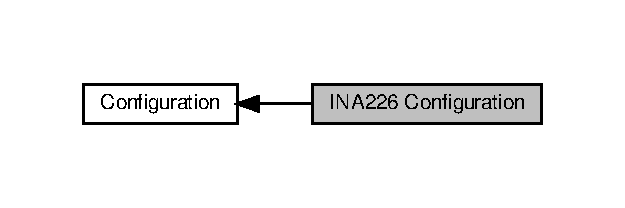
\includegraphics[width=300pt]{group__defines__ina226__configuration}
\end{center}
\end{figure}
\subsection*{Macros}
\begin{DoxyCompactItemize}
\item 
\#define \hyperlink{group__defines__ina226__configuration_gad742a86ac5089cdfc6bb385de8dae4de}{I\+N\+A\+\_\+\+A\+D\+DR}~0x40
\item 
\#define \hyperlink{group__defines__ina226__configuration_gae50e821d99cc5d3696877fd921049ea3}{I\+N\+A\+\_\+\+R\+S\+H\+U\+NT}~0.\+1
\item 
\#define \hyperlink{group__defines__ina226__configuration_ga30ad8caf4e8a6f008591d8a6e2ec6d9c}{I\+N\+A\+\_\+\+M\+A\+X\+\_\+\+C\+U\+R\+R\+E\+NT}~0.\+5
\item 
\#define \hyperlink{group__defines__ina226__configuration_ga03a691e35444e414c3256b234ec19abf}{I\+N\+A\+\_\+\+R\+E\+G\+\_\+\+M\+A\+N\+U\+F\+A\+C\+T\+U\+R\+E\+R\+\_\+\+ID}~0x\+FE
\item 
\#define \hyperlink{group__defines__ina226__configuration_gaa5387a1fef1c3a301c558d631851456a}{I\+N\+A\+\_\+\+M\+A\+N\+U\+F\+A\+C\+T\+U\+R\+E\+R\+\_\+\+ID}~0x5449
\end{DoxyCompactItemize}


\subsection{Detailed Description}
\begin{DoxyRefDesc}{Test}
\item[\hyperlink{test__test000019}{Test}](ID C\+O\+N\+F\+\_\+\+I\+N\+A226\+\_\+\+C\+O\+N\+F\+\_\+\+T0) (S\+EV 1) Check that the I\+N\+A226 can be connected to and gives the correct values.\end{DoxyRefDesc}


\subsection{Macro Definition Documentation}
\mbox{\Hypertarget{group__defines__ina226__configuration_gad742a86ac5089cdfc6bb385de8dae4de}\label{group__defines__ina226__configuration_gad742a86ac5089cdfc6bb385de8dae4de}} 
\index{I\+N\+A226 Configuration@{I\+N\+A226 Configuration}!I\+N\+A\+\_\+\+A\+D\+DR@{I\+N\+A\+\_\+\+A\+D\+DR}}
\index{I\+N\+A\+\_\+\+A\+D\+DR@{I\+N\+A\+\_\+\+A\+D\+DR}!I\+N\+A226 Configuration@{I\+N\+A226 Configuration}}
\subsubsection{\texorpdfstring{I\+N\+A\+\_\+\+A\+D\+DR}{INA\_ADDR}}
{\footnotesize\ttfamily \#define I\+N\+A\+\_\+\+A\+D\+DR~0x40}

The I2C address of the I\+N\+A226 module. 

Definition at line 114 of file configuration.\+h.

\mbox{\Hypertarget{group__defines__ina226__configuration_gaa5387a1fef1c3a301c558d631851456a}\label{group__defines__ina226__configuration_gaa5387a1fef1c3a301c558d631851456a}} 
\index{I\+N\+A226 Configuration@{I\+N\+A226 Configuration}!I\+N\+A\+\_\+\+M\+A\+N\+U\+F\+A\+C\+T\+U\+R\+E\+R\+\_\+\+ID@{I\+N\+A\+\_\+\+M\+A\+N\+U\+F\+A\+C\+T\+U\+R\+E\+R\+\_\+\+ID}}
\index{I\+N\+A\+\_\+\+M\+A\+N\+U\+F\+A\+C\+T\+U\+R\+E\+R\+\_\+\+ID@{I\+N\+A\+\_\+\+M\+A\+N\+U\+F\+A\+C\+T\+U\+R\+E\+R\+\_\+\+ID}!I\+N\+A226 Configuration@{I\+N\+A226 Configuration}}
\subsubsection{\texorpdfstring{I\+N\+A\+\_\+\+M\+A\+N\+U\+F\+A\+C\+T\+U\+R\+E\+R\+\_\+\+ID}{INA\_MANUFACTURER\_ID}}
{\footnotesize\ttfamily \#define I\+N\+A\+\_\+\+M\+A\+N\+U\+F\+A\+C\+T\+U\+R\+E\+R\+\_\+\+ID~0x5449}

I\+NA Manufacturer Identification Number (21577). 

Definition at line 118 of file configuration.\+h.

\mbox{\Hypertarget{group__defines__ina226__configuration_ga30ad8caf4e8a6f008591d8a6e2ec6d9c}\label{group__defines__ina226__configuration_ga30ad8caf4e8a6f008591d8a6e2ec6d9c}} 
\index{I\+N\+A226 Configuration@{I\+N\+A226 Configuration}!I\+N\+A\+\_\+\+M\+A\+X\+\_\+\+C\+U\+R\+R\+E\+NT@{I\+N\+A\+\_\+\+M\+A\+X\+\_\+\+C\+U\+R\+R\+E\+NT}}
\index{I\+N\+A\+\_\+\+M\+A\+X\+\_\+\+C\+U\+R\+R\+E\+NT@{I\+N\+A\+\_\+\+M\+A\+X\+\_\+\+C\+U\+R\+R\+E\+NT}!I\+N\+A226 Configuration@{I\+N\+A226 Configuration}}
\subsubsection{\texorpdfstring{I\+N\+A\+\_\+\+M\+A\+X\+\_\+\+C\+U\+R\+R\+E\+NT}{INA\_MAX\_CURRENT}}
{\footnotesize\ttfamily \#define I\+N\+A\+\_\+\+M\+A\+X\+\_\+\+C\+U\+R\+R\+E\+NT~0.\+5}

Maximum Current allowed (A). 

Definition at line 116 of file configuration.\+h.

\mbox{\Hypertarget{group__defines__ina226__configuration_ga03a691e35444e414c3256b234ec19abf}\label{group__defines__ina226__configuration_ga03a691e35444e414c3256b234ec19abf}} 
\index{I\+N\+A226 Configuration@{I\+N\+A226 Configuration}!I\+N\+A\+\_\+\+R\+E\+G\+\_\+\+M\+A\+N\+U\+F\+A\+C\+T\+U\+R\+E\+R\+\_\+\+ID@{I\+N\+A\+\_\+\+R\+E\+G\+\_\+\+M\+A\+N\+U\+F\+A\+C\+T\+U\+R\+E\+R\+\_\+\+ID}}
\index{I\+N\+A\+\_\+\+R\+E\+G\+\_\+\+M\+A\+N\+U\+F\+A\+C\+T\+U\+R\+E\+R\+\_\+\+ID@{I\+N\+A\+\_\+\+R\+E\+G\+\_\+\+M\+A\+N\+U\+F\+A\+C\+T\+U\+R\+E\+R\+\_\+\+ID}!I\+N\+A226 Configuration@{I\+N\+A226 Configuration}}
\subsubsection{\texorpdfstring{I\+N\+A\+\_\+\+R\+E\+G\+\_\+\+M\+A\+N\+U\+F\+A\+C\+T\+U\+R\+E\+R\+\_\+\+ID}{INA\_REG\_MANUFACTURER\_ID}}
{\footnotesize\ttfamily \#define I\+N\+A\+\_\+\+R\+E\+G\+\_\+\+M\+A\+N\+U\+F\+A\+C\+T\+U\+R\+E\+R\+\_\+\+ID~0x\+FE}

I\+NA Reg Manufacturer Identification Number (254). 

Definition at line 117 of file configuration.\+h.

\mbox{\Hypertarget{group__defines__ina226__configuration_gae50e821d99cc5d3696877fd921049ea3}\label{group__defines__ina226__configuration_gae50e821d99cc5d3696877fd921049ea3}} 
\index{I\+N\+A226 Configuration@{I\+N\+A226 Configuration}!I\+N\+A\+\_\+\+R\+S\+H\+U\+NT@{I\+N\+A\+\_\+\+R\+S\+H\+U\+NT}}
\index{I\+N\+A\+\_\+\+R\+S\+H\+U\+NT@{I\+N\+A\+\_\+\+R\+S\+H\+U\+NT}!I\+N\+A226 Configuration@{I\+N\+A226 Configuration}}
\subsubsection{\texorpdfstring{I\+N\+A\+\_\+\+R\+S\+H\+U\+NT}{INA\_RSHUNT}}
{\footnotesize\ttfamily \#define I\+N\+A\+\_\+\+R\+S\+H\+U\+NT~0.\+1}

Shunt resistor value (Ohm). 

Definition at line 115 of file configuration.\+h.


\hypertarget{group__defines__eeprom__address__map}{}\section{E\+E\+P\+R\+OM Address Map}
\label{group__defines__eeprom__address__map}\index{E\+E\+P\+R\+O\+M Address Map@{E\+E\+P\+R\+O\+M Address Map}}


\tabulinesep=1mm
\begin{longtabu} spread 0pt [c]{*{4}{|X[-1]}|}
\hline
\rowcolor{\tableheadbgcolor}\textbf{ Description}&\textbf{ Start Address}&\textbf{ End Address}&\textbf{ Length (bytes)  }\\\cline{1-4}
\endfirsthead
\hline
\endfoot
\hline
\rowcolor{\tableheadbgcolor}\textbf{ Description}&\textbf{ Start Address}&\textbf{ End Address}&\textbf{ Length (bytes)  }\\\cline{1-4}
\endhead
Deployment counter (uint8\+\_\+t).&0x0000&0x0000&1 \\\cline{1-4}
Power configuration (\hyperlink{unionpower_config__t}{power\+Config\+\_\+t}).&0x0001&0x0001&1 \\\cline{1-4}
First run (uint8\+\_\+t).&0x0002&0x0002&1 \\\cline{1-4}
Restart counter (uint16\+\_\+t).&0x0003&0x0004&2 \\\cline{1-4}
F\+SK receive window length (uint8\+\_\+t).&0x0005&0x0005&1 \\\cline{1-4}
Lo\+Ra receive window length (uint8\+\_\+t).&0x0006&0x0006&1 \\\cline{1-4}
Seconds elapsed since last reset (uint32\+\_\+t).&0x0007&0x000A&4 \\\cline{1-4}
Number of main loop iterations (uint8\+\_\+t).&0x000B&0x000B&1 \\\cline{1-4}
Number of received valid Lo\+Ra frames (uint16\+\_\+t).&0x000C&0x000D&2 \\\cline{1-4}
Number of received invalid Lo\+Ra frames (uint16\+\_\+t).&0x000E&0x000F&2 \\\cline{1-4}
Number of received valid F\+SK frames (uint16\+\_\+t).&0x0010&0x0011&2 \\\cline{1-4}
Number of received invalid F\+SK frames (uint16\+\_\+t).&0x0012&0x0013&2 \\\cline{1-4}
Length of callsign (uint8\+\_\+t).&0x0014&0x0014&1 \\\cline{1-4}
Callsign (C-\/string, max M\+A\+X\+\_\+\+S\+T\+R\+I\+N\+G\+\_\+\+L\+E\+N\+G\+TH bytes).&0x00015&0x0035&M\+A\+X\+\_\+\+S\+T\+R\+I\+N\+G\+\_\+\+L\+E\+N\+G\+TH \\\cline{1-4}
Charging voltage stats (min -\/ avg -\/ max, 3x uint8\+\_\+t).&0x0040&0x0042&3 \\\cline{1-4}
Charging current stats (min -\/ avg -\/ max, 3x int16\+\_\+t).&0x0043&0x0048&6 \\\cline{1-4}
Battery voltage stats (min -\/ avg -\/ max, 3x uint8\+\_\+t).&0x0049&0x004B&3 \\\cline{1-4}
Solar cell A voltage stats (min -\/ avg -\/ max, 3x uint8\+\_\+t).&0x004C&0x004E&3 \\\cline{1-4}
Solar cell B voltage stats (min -\/ avg -\/ max, 3x uint8\+\_\+t).&0x004F&0x0051&3 \\\cline{1-4}
Solar cell C voltage stats (min -\/ avg -\/ max, 3x uint8\+\_\+t).&0x0052&0x0054&3 \\\cline{1-4}
Battery temperature stats (min -\/ avg -\/ max, 3x int16\+\_\+t).&0x0055&0x005A&6 \\\cline{1-4}
Board temperature stats (min -\/ avg -\/ max, 3x int16\+\_\+t).&0x005B&0x0060&6 \\\cline{1-4}
M\+CU temperature stats (min -\/ avg -\/ max, 3x int8\+\_\+t).&0x0061&0x0063&3 \\\cline{1-4}
Total&&&72 \\\cline{1-4}
\end{longtabu}
 


Collaboration diagram for E\+E\+P\+R\+OM Address Map\+:
\nopagebreak
\begin{figure}[H]
\begin{center}
\leavevmode
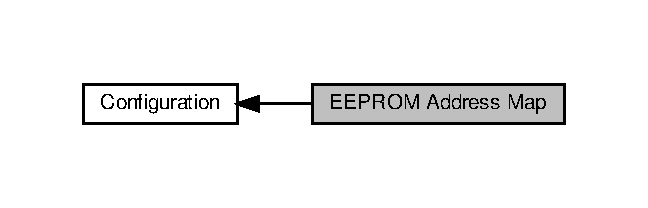
\includegraphics[width=311pt]{group__defines__eeprom__address__map}
\end{center}
\end{figure}
\subsection*{Macros}
\begin{DoxyCompactItemize}
\item 
\mbox{\Hypertarget{group__defines__eeprom__address__map_gaf8c8716a907b10b7d07c1d05f925915b}\label{group__defines__eeprom__address__map_gaf8c8716a907b10b7d07c1d05f925915b}} 
\#define \hyperlink{group__defines__eeprom__address__map_gaf8c8716a907b10b7d07c1d05f925915b}{E\+E\+P\+R\+O\+M\+\_\+\+D\+E\+P\+L\+O\+Y\+M\+E\+N\+T\+\_\+\+C\+O\+U\+N\+T\+E\+R\+\_\+\+A\+D\+DR}~0x0000
\begin{DoxyCompactList}\small\item\em \tabulinesep=1mm
\begin{longtabu} spread 0pt [c]{*{2}{|X[-1]}|}
\hline
\rowcolor{\tableheadbgcolor}\textbf{ Start Address}&\textbf{ End Address  }\\\cline{1-2}
\endfirsthead
\hline
\endfoot
\hline
\rowcolor{\tableheadbgcolor}\textbf{ Start Address}&\textbf{ End Address  }\\\cline{1-2}
\endhead
0x0000&0x0000 \\\cline{1-2}
\end{longtabu}
\end{DoxyCompactList}\item 
\mbox{\Hypertarget{group__defines__eeprom__address__map_gad0b4d3e4a81df862dfe961caaa6432c2}\label{group__defines__eeprom__address__map_gad0b4d3e4a81df862dfe961caaa6432c2}} 
\#define \hyperlink{group__defines__eeprom__address__map_gad0b4d3e4a81df862dfe961caaa6432c2}{E\+E\+P\+R\+O\+M\+\_\+\+P\+O\+W\+E\+R\+\_\+\+C\+O\+N\+F\+I\+G\+\_\+\+A\+D\+DR}~0x0001
\begin{DoxyCompactList}\small\item\em \tabulinesep=1mm
\begin{longtabu} spread 0pt [c]{*{2}{|X[-1]}|}
\hline
\rowcolor{\tableheadbgcolor}\textbf{ Start Address}&\textbf{ End Address  }\\\cline{1-2}
\endfirsthead
\hline
\endfoot
\hline
\rowcolor{\tableheadbgcolor}\textbf{ Start Address}&\textbf{ End Address  }\\\cline{1-2}
\endhead
0x0001&0x0001 \\\cline{1-2}
\end{longtabu}
\end{DoxyCompactList}\item 
\mbox{\Hypertarget{group__defines__eeprom__address__map_gaaef7c132060420925a4b03f0763d1c19}\label{group__defines__eeprom__address__map_gaaef7c132060420925a4b03f0763d1c19}} 
\#define \hyperlink{group__defines__eeprom__address__map_gaaef7c132060420925a4b03f0763d1c19}{E\+E\+P\+R\+O\+M\+\_\+\+F\+I\+R\+S\+T\+\_\+\+R\+U\+N\+\_\+\+A\+D\+DR}~0x0002
\begin{DoxyCompactList}\small\item\em \tabulinesep=1mm
\begin{longtabu} spread 0pt [c]{*{2}{|X[-1]}|}
\hline
\rowcolor{\tableheadbgcolor}\textbf{ Start Address}&\textbf{ End Address  }\\\cline{1-2}
\endfirsthead
\hline
\endfoot
\hline
\rowcolor{\tableheadbgcolor}\textbf{ Start Address}&\textbf{ End Address  }\\\cline{1-2}
\endhead
0x0002&0x0002 \\\cline{1-2}
\end{longtabu}
\end{DoxyCompactList}\item 
\mbox{\Hypertarget{group__defines__eeprom__address__map_gad9936577552bbcc87b8a57b75759f01f}\label{group__defines__eeprom__address__map_gad9936577552bbcc87b8a57b75759f01f}} 
\#define \hyperlink{group__defines__eeprom__address__map_gad9936577552bbcc87b8a57b75759f01f}{E\+E\+P\+R\+O\+M\+\_\+\+R\+E\+S\+T\+A\+R\+T\+\_\+\+C\+O\+U\+N\+T\+E\+R\+\_\+\+A\+D\+DR}~0x0003
\begin{DoxyCompactList}\small\item\em \tabulinesep=1mm
\begin{longtabu} spread 0pt [c]{*{2}{|X[-1]}|}
\hline
\rowcolor{\tableheadbgcolor}\textbf{ Start Address}&\textbf{ End Address  }\\\cline{1-2}
\endfirsthead
\hline
\endfoot
\hline
\rowcolor{\tableheadbgcolor}\textbf{ Start Address}&\textbf{ End Address  }\\\cline{1-2}
\endhead
0x0003&0x0004 \\\cline{1-2}
\end{longtabu}
\end{DoxyCompactList}\item 
\mbox{\Hypertarget{group__defines__eeprom__address__map_gab989de4b765c220d4eaaa36c0d182fd5}\label{group__defines__eeprom__address__map_gab989de4b765c220d4eaaa36c0d182fd5}} 
\#define \hyperlink{group__defines__eeprom__address__map_gab989de4b765c220d4eaaa36c0d182fd5}{E\+E\+P\+R\+O\+M\+\_\+\+F\+S\+K\+\_\+\+R\+E\+C\+E\+I\+V\+E\+\_\+\+L\+E\+N\+\_\+\+A\+D\+DR}~0x0005
\begin{DoxyCompactList}\small\item\em \tabulinesep=1mm
\begin{longtabu} spread 0pt [c]{*{2}{|X[-1]}|}
\hline
\rowcolor{\tableheadbgcolor}\textbf{ Start Address}&\textbf{ End Address  }\\\cline{1-2}
\endfirsthead
\hline
\endfoot
\hline
\rowcolor{\tableheadbgcolor}\textbf{ Start Address}&\textbf{ End Address  }\\\cline{1-2}
\endhead
0x0005&0x0005 \\\cline{1-2}
\end{longtabu}
\end{DoxyCompactList}\item 
\mbox{\Hypertarget{group__defines__eeprom__address__map_ga110fef28d82a0c77f7134cef20b16008}\label{group__defines__eeprom__address__map_ga110fef28d82a0c77f7134cef20b16008}} 
\#define \hyperlink{group__defines__eeprom__address__map_ga110fef28d82a0c77f7134cef20b16008}{E\+E\+P\+R\+O\+M\+\_\+\+L\+O\+R\+A\+\_\+\+R\+E\+C\+E\+I\+V\+E\+\_\+\+L\+E\+N\+\_\+\+A\+D\+DR}~0x0006
\begin{DoxyCompactList}\small\item\em \tabulinesep=1mm
\begin{longtabu} spread 0pt [c]{*{2}{|X[-1]}|}
\hline
\rowcolor{\tableheadbgcolor}\textbf{ Start Address}&\textbf{ End Address  }\\\cline{1-2}
\endfirsthead
\hline
\endfoot
\hline
\rowcolor{\tableheadbgcolor}\textbf{ Start Address}&\textbf{ End Address  }\\\cline{1-2}
\endhead
0x0006&0x0006 \\\cline{1-2}
\end{longtabu}
\end{DoxyCompactList}\item 
\mbox{\Hypertarget{group__defines__eeprom__address__map_ga8bd2bb8a04777f7fb9c24db8027e9a51}\label{group__defines__eeprom__address__map_ga8bd2bb8a04777f7fb9c24db8027e9a51}} 
\#define \hyperlink{group__defines__eeprom__address__map_ga8bd2bb8a04777f7fb9c24db8027e9a51}{E\+E\+P\+R\+O\+M\+\_\+\+U\+P\+T\+I\+M\+E\+\_\+\+C\+O\+U\+N\+T\+E\+R\+\_\+\+A\+D\+DR}~0x0007
\begin{DoxyCompactList}\small\item\em \tabulinesep=1mm
\begin{longtabu} spread 0pt [c]{*{2}{|X[-1]}|}
\hline
\rowcolor{\tableheadbgcolor}\textbf{ Start Address}&\textbf{ End Address  }\\\cline{1-2}
\endfirsthead
\hline
\endfoot
\hline
\rowcolor{\tableheadbgcolor}\textbf{ Start Address}&\textbf{ End Address  }\\\cline{1-2}
\endhead
0x0007&0x000A \\\cline{1-2}
\end{longtabu}
\end{DoxyCompactList}\item 
\mbox{\Hypertarget{group__defines__eeprom__address__map_gaa512d20cb045b2b6e27676f5d3c9547f}\label{group__defines__eeprom__address__map_gaa512d20cb045b2b6e27676f5d3c9547f}} 
\#define \hyperlink{group__defines__eeprom__address__map_gaa512d20cb045b2b6e27676f5d3c9547f}{E\+E\+P\+R\+O\+M\+\_\+\+L\+O\+O\+P\+\_\+\+C\+O\+U\+N\+T\+ER}~0x000B
\begin{DoxyCompactList}\small\item\em Loop counter -\/ only used to determine when to transmit full Morse beacon, so it doesn\textquotesingle{}t matter when it overflows. \tabulinesep=1mm
\begin{longtabu} spread 0pt [c]{*{2}{|X[-1]}|}
\hline
\rowcolor{\tableheadbgcolor}\textbf{ Start Address}&\textbf{ End Address  }\\\cline{1-2}
\endfirsthead
\hline
\endfoot
\hline
\rowcolor{\tableheadbgcolor}\textbf{ Start Address}&\textbf{ End Address  }\\\cline{1-2}
\endhead
0x000B&0x000B \\\cline{1-2}
\end{longtabu}
\end{DoxyCompactList}\item 
\mbox{\Hypertarget{group__defines__eeprom__address__map_gaa877b7e655f92a71a256bfb4406d4be7}\label{group__defines__eeprom__address__map_gaa877b7e655f92a71a256bfb4406d4be7}} 
\#define \hyperlink{group__defines__eeprom__address__map_gaa877b7e655f92a71a256bfb4406d4be7}{E\+E\+P\+R\+O\+M\+\_\+\+L\+O\+R\+A\+\_\+\+V\+A\+L\+I\+D\+\_\+\+C\+O\+U\+N\+T\+E\+R\+\_\+\+A\+D\+DR}~0x000C
\begin{DoxyCompactList}\small\item\em \tabulinesep=1mm
\begin{longtabu} spread 0pt [c]{*{2}{|X[-1]}|}
\hline
\rowcolor{\tableheadbgcolor}\textbf{ Start Address}&\textbf{ End Address  }\\\cline{1-2}
\endfirsthead
\hline
\endfoot
\hline
\rowcolor{\tableheadbgcolor}\textbf{ Start Address}&\textbf{ End Address  }\\\cline{1-2}
\endhead
0x000C&0x000D \\\cline{1-2}
\end{longtabu}
\end{DoxyCompactList}\item 
\mbox{\Hypertarget{group__defines__eeprom__address__map_ga09e7db19ac65e0c28bae5b46f25ffe36}\label{group__defines__eeprom__address__map_ga09e7db19ac65e0c28bae5b46f25ffe36}} 
\#define \hyperlink{group__defines__eeprom__address__map_ga09e7db19ac65e0c28bae5b46f25ffe36}{E\+E\+P\+R\+O\+M\+\_\+\+L\+O\+R\+A\+\_\+\+I\+N\+V\+A\+L\+I\+D\+\_\+\+C\+O\+U\+N\+T\+E\+R\+\_\+\+A\+D\+DR}~0x000E
\begin{DoxyCompactList}\small\item\em \tabulinesep=1mm
\begin{longtabu} spread 0pt [c]{*{2}{|X[-1]}|}
\hline
\rowcolor{\tableheadbgcolor}\textbf{ Start Address}&\textbf{ End Address  }\\\cline{1-2}
\endfirsthead
\hline
\endfoot
\hline
\rowcolor{\tableheadbgcolor}\textbf{ Start Address}&\textbf{ End Address  }\\\cline{1-2}
\endhead
0x000E&0x000F \\\cline{1-2}
\end{longtabu}
\end{DoxyCompactList}\item 
\mbox{\Hypertarget{group__defines__eeprom__address__map_gae0a7ddd98b2a6e5c878c65c223e8d1d9}\label{group__defines__eeprom__address__map_gae0a7ddd98b2a6e5c878c65c223e8d1d9}} 
\#define \hyperlink{group__defines__eeprom__address__map_gae0a7ddd98b2a6e5c878c65c223e8d1d9}{E\+E\+P\+R\+O\+M\+\_\+\+F\+S\+K\+\_\+\+V\+A\+L\+I\+D\+\_\+\+C\+O\+U\+N\+T\+E\+R\+\_\+\+A\+D\+DR}~0x0010
\begin{DoxyCompactList}\small\item\em \tabulinesep=1mm
\begin{longtabu} spread 0pt [c]{*{2}{|X[-1]}|}
\hline
\rowcolor{\tableheadbgcolor}\textbf{ Start Address}&\textbf{ End Address  }\\\cline{1-2}
\endfirsthead
\hline
\endfoot
\hline
\rowcolor{\tableheadbgcolor}\textbf{ Start Address}&\textbf{ End Address  }\\\cline{1-2}
\endhead
0x0010&0x0011 \\\cline{1-2}
\end{longtabu}
\end{DoxyCompactList}\item 
\mbox{\Hypertarget{group__defines__eeprom__address__map_ga6fb56c8041b356cfc0e4de4731eeb4fd}\label{group__defines__eeprom__address__map_ga6fb56c8041b356cfc0e4de4731eeb4fd}} 
\#define \hyperlink{group__defines__eeprom__address__map_ga6fb56c8041b356cfc0e4de4731eeb4fd}{E\+E\+P\+R\+O\+M\+\_\+\+F\+S\+K\+\_\+\+I\+N\+V\+A\+L\+I\+D\+\_\+\+C\+O\+U\+N\+T\+E\+R\+\_\+\+A\+D\+DR}~0x0012
\begin{DoxyCompactList}\small\item\em \tabulinesep=1mm
\begin{longtabu} spread 0pt [c]{*{2}{|X[-1]}|}
\hline
\rowcolor{\tableheadbgcolor}\textbf{ Start Address}&\textbf{ End Address  }\\\cline{1-2}
\endfirsthead
\hline
\endfoot
\hline
\rowcolor{\tableheadbgcolor}\textbf{ Start Address}&\textbf{ End Address  }\\\cline{1-2}
\endhead
0x0012&0x0013 \\\cline{1-2}
\end{longtabu}
\end{DoxyCompactList}\item 
\mbox{\Hypertarget{group__defines__eeprom__address__map_ga84c346e7353930c5977017a1efa4ff55}\label{group__defines__eeprom__address__map_ga84c346e7353930c5977017a1efa4ff55}} 
\#define \hyperlink{group__defines__eeprom__address__map_ga84c346e7353930c5977017a1efa4ff55}{E\+E\+P\+R\+O\+M\+\_\+\+C\+A\+L\+L\+S\+I\+G\+N\+\_\+\+L\+E\+N\+\_\+\+A\+D\+DR}~0x0014
\begin{DoxyCompactList}\small\item\em \tabulinesep=1mm
\begin{longtabu} spread 0pt [c]{*{2}{|X[-1]}|}
\hline
\rowcolor{\tableheadbgcolor}\textbf{ Start Address}&\textbf{ End Address  }\\\cline{1-2}
\endfirsthead
\hline
\endfoot
\hline
\rowcolor{\tableheadbgcolor}\textbf{ Start Address}&\textbf{ End Address  }\\\cline{1-2}
\endhead
0x00014&0x00014 \\\cline{1-2}
\end{longtabu}
\end{DoxyCompactList}\item 
\mbox{\Hypertarget{group__defines__eeprom__address__map_ga914e5eca76c425eef3794078a440ef89}\label{group__defines__eeprom__address__map_ga914e5eca76c425eef3794078a440ef89}} 
\#define \hyperlink{group__defines__eeprom__address__map_ga914e5eca76c425eef3794078a440ef89}{E\+E\+P\+R\+O\+M\+\_\+\+C\+A\+L\+L\+S\+I\+G\+N\+\_\+\+A\+D\+DR}~0x0015
\begin{DoxyCompactList}\small\item\em \tabulinesep=1mm
\begin{longtabu} spread 0pt [c]{*{2}{|X[-1]}|}
\hline
\rowcolor{\tableheadbgcolor}\textbf{ Start Address}&\textbf{ End Address  }\\\cline{1-2}
\endfirsthead
\hline
\endfoot
\hline
\rowcolor{\tableheadbgcolor}\textbf{ Start Address}&\textbf{ End Address  }\\\cline{1-2}
\endhead
0x0015&0x0035 \\\cline{1-2}
\end{longtabu}
\end{DoxyCompactList}\item 
\mbox{\Hypertarget{group__defines__eeprom__address__map_ga18497ed096651b6d9fb7d0cb0afc43d7}\label{group__defines__eeprom__address__map_ga18497ed096651b6d9fb7d0cb0afc43d7}} 
\#define \hyperlink{group__defines__eeprom__address__map_ga18497ed096651b6d9fb7d0cb0afc43d7}{E\+E\+P\+R\+O\+M\+\_\+\+C\+H\+A\+R\+G\+I\+N\+G\+\_\+\+V\+O\+L\+T\+A\+G\+E\+\_\+\+S\+T\+A\+T\+S\+\_\+\+A\+D\+DR}~0x0040
\begin{DoxyCompactList}\small\item\em \tabulinesep=1mm
\begin{longtabu} spread 0pt [c]{*{2}{|X[-1]}|}
\hline
\rowcolor{\tableheadbgcolor}\textbf{ Start Address}&\textbf{ End Address  }\\\cline{1-2}
\endfirsthead
\hline
\endfoot
\hline
\rowcolor{\tableheadbgcolor}\textbf{ Start Address}&\textbf{ End Address  }\\\cline{1-2}
\endhead
0x0040&0x0042 \\\cline{1-2}
\end{longtabu}
\end{DoxyCompactList}\item 
\mbox{\Hypertarget{group__defines__eeprom__address__map_gaded138a94dfe781c99f664d6ce3be8d0}\label{group__defines__eeprom__address__map_gaded138a94dfe781c99f664d6ce3be8d0}} 
\#define \hyperlink{group__defines__eeprom__address__map_gaded138a94dfe781c99f664d6ce3be8d0}{E\+E\+P\+R\+O\+M\+\_\+\+C\+H\+A\+R\+G\+I\+N\+G\+\_\+\+C\+U\+R\+R\+E\+N\+T\+\_\+\+S\+T\+A\+T\+S\+\_\+\+A\+D\+DR}~0x0043
\begin{DoxyCompactList}\small\item\em \tabulinesep=1mm
\begin{longtabu} spread 0pt [c]{*{2}{|X[-1]}|}
\hline
\rowcolor{\tableheadbgcolor}\textbf{ Start Address}&\textbf{ End Address  }\\\cline{1-2}
\endfirsthead
\hline
\endfoot
\hline
\rowcolor{\tableheadbgcolor}\textbf{ Start Address}&\textbf{ End Address  }\\\cline{1-2}
\endhead
0x0043&0x0048 \\\cline{1-2}
\end{longtabu}
\end{DoxyCompactList}\item 
\mbox{\Hypertarget{group__defines__eeprom__address__map_ga3f624256f4e308657f4c4053c64f0feb}\label{group__defines__eeprom__address__map_ga3f624256f4e308657f4c4053c64f0feb}} 
\#define \hyperlink{group__defines__eeprom__address__map_ga3f624256f4e308657f4c4053c64f0feb}{E\+E\+P\+R\+O\+M\+\_\+\+B\+A\+T\+T\+E\+R\+Y\+\_\+\+V\+O\+L\+T\+A\+G\+E\+\_\+\+S\+T\+A\+T\+S\+\_\+\+A\+D\+DR}~0x0049
\begin{DoxyCompactList}\small\item\em \tabulinesep=1mm
\begin{longtabu} spread 0pt [c]{*{2}{|X[-1]}|}
\hline
\rowcolor{\tableheadbgcolor}\textbf{ Start Address}&\textbf{ End Address  }\\\cline{1-2}
\endfirsthead
\hline
\endfoot
\hline
\rowcolor{\tableheadbgcolor}\textbf{ Start Address}&\textbf{ End Address  }\\\cline{1-2}
\endhead
0x0049&0x004B \\\cline{1-2}
\end{longtabu}
\end{DoxyCompactList}\item 
\mbox{\Hypertarget{group__defines__eeprom__address__map_gaa84e17318d3dbe0d8d14ce87c2157774}\label{group__defines__eeprom__address__map_gaa84e17318d3dbe0d8d14ce87c2157774}} 
\#define \hyperlink{group__defines__eeprom__address__map_gaa84e17318d3dbe0d8d14ce87c2157774}{E\+E\+P\+R\+O\+M\+\_\+\+C\+E\+L\+L\+\_\+\+A\+\_\+\+V\+O\+L\+T\+A\+G\+E\+\_\+\+S\+T\+A\+T\+S\+\_\+\+A\+D\+DR}~0x004C
\begin{DoxyCompactList}\small\item\em \tabulinesep=1mm
\begin{longtabu} spread 0pt [c]{*{2}{|X[-1]}|}
\hline
\rowcolor{\tableheadbgcolor}\textbf{ Start Address}&\textbf{ End Address  }\\\cline{1-2}
\endfirsthead
\hline
\endfoot
\hline
\rowcolor{\tableheadbgcolor}\textbf{ Start Address}&\textbf{ End Address  }\\\cline{1-2}
\endhead
0x004C&0x004E \\\cline{1-2}
\end{longtabu}
\end{DoxyCompactList}\item 
\mbox{\Hypertarget{group__defines__eeprom__address__map_ga94346f859875a8ba8b32e579633678cc}\label{group__defines__eeprom__address__map_ga94346f859875a8ba8b32e579633678cc}} 
\#define \hyperlink{group__defines__eeprom__address__map_ga94346f859875a8ba8b32e579633678cc}{E\+E\+P\+R\+O\+M\+\_\+\+C\+E\+L\+L\+\_\+\+B\+\_\+\+V\+O\+L\+T\+A\+G\+E\+\_\+\+S\+T\+A\+T\+S\+\_\+\+A\+D\+DR}~0x004F
\begin{DoxyCompactList}\small\item\em \tabulinesep=1mm
\begin{longtabu} spread 0pt [c]{*{2}{|X[-1]}|}
\hline
\rowcolor{\tableheadbgcolor}\textbf{ Start Address}&\textbf{ End Address  }\\\cline{1-2}
\endfirsthead
\hline
\endfoot
\hline
\rowcolor{\tableheadbgcolor}\textbf{ Start Address}&\textbf{ End Address  }\\\cline{1-2}
\endhead
0x004F&0x0051 \\\cline{1-2}
\end{longtabu}
\end{DoxyCompactList}\item 
\mbox{\Hypertarget{group__defines__eeprom__address__map_gaed59c9e0cd2b68c47afd39ec1954b5e6}\label{group__defines__eeprom__address__map_gaed59c9e0cd2b68c47afd39ec1954b5e6}} 
\#define \hyperlink{group__defines__eeprom__address__map_gaed59c9e0cd2b68c47afd39ec1954b5e6}{E\+E\+P\+R\+O\+M\+\_\+\+C\+E\+L\+L\+\_\+\+C\+\_\+\+V\+O\+L\+T\+A\+G\+E\+\_\+\+S\+T\+A\+T\+S\+\_\+\+A\+D\+DR}~0x0052
\begin{DoxyCompactList}\small\item\em \tabulinesep=1mm
\begin{longtabu} spread 0pt [c]{*{2}{|X[-1]}|}
\hline
\rowcolor{\tableheadbgcolor}\textbf{ Start Address}&\textbf{ End Address  }\\\cline{1-2}
\endfirsthead
\hline
\endfoot
\hline
\rowcolor{\tableheadbgcolor}\textbf{ Start Address}&\textbf{ End Address  }\\\cline{1-2}
\endhead
0x0052&0x0054 \\\cline{1-2}
\end{longtabu}
\end{DoxyCompactList}\item 
\mbox{\Hypertarget{group__defines__eeprom__address__map_ga8c5548d7c7e72c9974dbc3a4e670e1cf}\label{group__defines__eeprom__address__map_ga8c5548d7c7e72c9974dbc3a4e670e1cf}} 
\#define \hyperlink{group__defines__eeprom__address__map_ga8c5548d7c7e72c9974dbc3a4e670e1cf}{E\+E\+P\+R\+O\+M\+\_\+\+B\+A\+T\+T\+E\+R\+Y\+\_\+\+T\+E\+M\+P\+\_\+\+S\+T\+A\+T\+S\+\_\+\+A\+D\+DR}~0x0055
\begin{DoxyCompactList}\small\item\em \tabulinesep=1mm
\begin{longtabu} spread 0pt [c]{*{2}{|X[-1]}|}
\hline
\rowcolor{\tableheadbgcolor}\textbf{ Start Address}&\textbf{ End Address  }\\\cline{1-2}
\endfirsthead
\hline
\endfoot
\hline
\rowcolor{\tableheadbgcolor}\textbf{ Start Address}&\textbf{ End Address  }\\\cline{1-2}
\endhead
0x0055&0x005A \\\cline{1-2}
\end{longtabu}
\end{DoxyCompactList}\item 
\mbox{\Hypertarget{group__defines__eeprom__address__map_ga400ff3c988dbb629cd17e1e7befee3bc}\label{group__defines__eeprom__address__map_ga400ff3c988dbb629cd17e1e7befee3bc}} 
\#define \hyperlink{group__defines__eeprom__address__map_ga400ff3c988dbb629cd17e1e7befee3bc}{E\+E\+P\+R\+O\+M\+\_\+\+B\+O\+A\+R\+D\+\_\+\+T\+E\+M\+P\+\_\+\+S\+T\+A\+T\+S\+\_\+\+A\+D\+DR}~0x005B
\begin{DoxyCompactList}\small\item\em \tabulinesep=1mm
\begin{longtabu} spread 0pt [c]{*{2}{|X[-1]}|}
\hline
\rowcolor{\tableheadbgcolor}\textbf{ Start Address}&\textbf{ End Address  }\\\cline{1-2}
\endfirsthead
\hline
\endfoot
\hline
\rowcolor{\tableheadbgcolor}\textbf{ Start Address}&\textbf{ End Address  }\\\cline{1-2}
\endhead
0x005B&0x0060 \\\cline{1-2}
\end{longtabu}
\end{DoxyCompactList}\item 
\mbox{\Hypertarget{group__defines__eeprom__address__map_gaf3993737bc8bdb1ee7aac5a636fc6936}\label{group__defines__eeprom__address__map_gaf3993737bc8bdb1ee7aac5a636fc6936}} 
\#define \hyperlink{group__defines__eeprom__address__map_gaf3993737bc8bdb1ee7aac5a636fc6936}{E\+E\+P\+R\+O\+M\+\_\+\+M\+C\+U\+\_\+\+T\+E\+M\+P\+\_\+\+S\+T\+A\+T\+S\+\_\+\+A\+D\+DR}~0x0061
\begin{DoxyCompactList}\small\item\em \tabulinesep=1mm
\begin{longtabu} spread 0pt [c]{*{2}{|X[-1]}|}
\hline
\rowcolor{\tableheadbgcolor}\textbf{ Start Address}&\textbf{ End Address  }\\\cline{1-2}
\endfirsthead
\hline
\endfoot
\hline
\rowcolor{\tableheadbgcolor}\textbf{ Start Address}&\textbf{ End Address  }\\\cline{1-2}
\endhead
0x0061&0x0063 \\\cline{1-2}
\end{longtabu}
\end{DoxyCompactList}\end{DoxyCompactItemize}


\subsection{Detailed Description}
\tabulinesep=1mm
\begin{longtabu} spread 0pt [c]{*{4}{|X[-1]}|}
\hline
\rowcolor{\tableheadbgcolor}\textbf{ Description}&\textbf{ Start Address}&\textbf{ End Address}&\textbf{ Length (bytes)  }\\\cline{1-4}
\endfirsthead
\hline
\endfoot
\hline
\rowcolor{\tableheadbgcolor}\textbf{ Description}&\textbf{ Start Address}&\textbf{ End Address}&\textbf{ Length (bytes)  }\\\cline{1-4}
\endhead
Deployment counter (uint8\+\_\+t).&0x0000&0x0000&1 \\\cline{1-4}
Power configuration (\hyperlink{unionpower_config__t}{power\+Config\+\_\+t}).&0x0001&0x0001&1 \\\cline{1-4}
First run (uint8\+\_\+t).&0x0002&0x0002&1 \\\cline{1-4}
Restart counter (uint16\+\_\+t).&0x0003&0x0004&2 \\\cline{1-4}
F\+SK receive window length (uint8\+\_\+t).&0x0005&0x0005&1 \\\cline{1-4}
Lo\+Ra receive window length (uint8\+\_\+t).&0x0006&0x0006&1 \\\cline{1-4}
Seconds elapsed since last reset (uint32\+\_\+t).&0x0007&0x000A&4 \\\cline{1-4}
Number of main loop iterations (uint8\+\_\+t).&0x000B&0x000B&1 \\\cline{1-4}
Number of received valid Lo\+Ra frames (uint16\+\_\+t).&0x000C&0x000D&2 \\\cline{1-4}
Number of received invalid Lo\+Ra frames (uint16\+\_\+t).&0x000E&0x000F&2 \\\cline{1-4}
Number of received valid F\+SK frames (uint16\+\_\+t).&0x0010&0x0011&2 \\\cline{1-4}
Number of received invalid F\+SK frames (uint16\+\_\+t).&0x0012&0x0013&2 \\\cline{1-4}
Length of callsign (uint8\+\_\+t).&0x0014&0x0014&1 \\\cline{1-4}
Callsign (C-\/string, max M\+A\+X\+\_\+\+S\+T\+R\+I\+N\+G\+\_\+\+L\+E\+N\+G\+TH bytes).&0x00015&0x0035&M\+A\+X\+\_\+\+S\+T\+R\+I\+N\+G\+\_\+\+L\+E\+N\+G\+TH \\\cline{1-4}
Charging voltage stats (min -\/ avg -\/ max, 3x uint8\+\_\+t).&0x0040&0x0042&3 \\\cline{1-4}
Charging current stats (min -\/ avg -\/ max, 3x int16\+\_\+t).&0x0043&0x0048&6 \\\cline{1-4}
Battery voltage stats (min -\/ avg -\/ max, 3x uint8\+\_\+t).&0x0049&0x004B&3 \\\cline{1-4}
Solar cell A voltage stats (min -\/ avg -\/ max, 3x uint8\+\_\+t).&0x004C&0x004E&3 \\\cline{1-4}
Solar cell B voltage stats (min -\/ avg -\/ max, 3x uint8\+\_\+t).&0x004F&0x0051&3 \\\cline{1-4}
Solar cell C voltage stats (min -\/ avg -\/ max, 3x uint8\+\_\+t).&0x0052&0x0054&3 \\\cline{1-4}
Battery temperature stats (min -\/ avg -\/ max, 3x int16\+\_\+t).&0x0055&0x005A&6 \\\cline{1-4}
Board temperature stats (min -\/ avg -\/ max, 3x int16\+\_\+t).&0x005B&0x0060&6 \\\cline{1-4}
M\+CU temperature stats (min -\/ avg -\/ max, 3x int8\+\_\+t).&0x0061&0x0063&3 \\\cline{1-4}
Total&&&72 \\\cline{1-4}
\end{longtabu}


\begin{DoxyRefDesc}{Test}
\item[\hyperlink{test__test000020}{Test}](ID C\+O\+N\+F\+\_\+\+E\+E\+P\+R\+O\+M\+\_\+\+A\+D\+D\+R\+\_\+\+M\+A\+P\+\_\+\+T0) (S\+EV 1) Check that E\+E\+P\+R\+O\+M\+\_\+\+D\+E\+P\+L\+O\+Y\+M\+E\+N\+T\+\_\+\+C\+O\+U\+N\+T\+E\+R\+\_\+\+A\+D\+DR is functional, including restarts. 

(ID C\+O\+N\+F\+\_\+\+E\+E\+P\+R\+O\+M\+\_\+\+A\+D\+D\+R\+\_\+\+M\+A\+P\+\_\+\+T1) (S\+EV 1) Check that E\+E\+P\+R\+O\+M\+\_\+\+P\+O\+W\+E\+R\+\_\+\+C\+O\+N\+F\+I\+G\+\_\+\+A\+D\+DR is functional, including restarts. 

(ID C\+O\+N\+F\+\_\+\+E\+E\+P\+R\+O\+M\+\_\+\+A\+D\+D\+R\+\_\+\+M\+A\+P\+\_\+\+T2) (S\+EV 1) Check that E\+E\+P\+R\+O\+M\+\_\+\+F\+I\+R\+S\+T\+\_\+\+R\+U\+N\+\_\+\+A\+D\+DR is functional, including restarts. 

(ID C\+O\+N\+F\+\_\+\+E\+E\+P\+R\+O\+M\+\_\+\+A\+D\+D\+R\+\_\+\+M\+A\+P\+\_\+\+T3) (S\+EV 1) Check that E\+E\+P\+R\+O\+M\+\_\+\+R\+E\+S\+T\+A\+R\+T\+\_\+\+C\+O\+U\+N\+T\+E\+R\+\_\+\+A\+D\+DR is functional, including restarts. 

(ID C\+O\+N\+F\+\_\+\+E\+E\+P\+R\+O\+M\+\_\+\+A\+D\+D\+R\+\_\+\+M\+A\+P\+\_\+\+T4) (S\+EV 1) Check that E\+E\+P\+R\+O\+M\+\_\+\+C\+A\+L\+L\+S\+I\+G\+N\+\_\+\+L\+E\+N\+\_\+\+A\+D\+DR is functional, including restarts. 

(ID C\+O\+N\+F\+\_\+\+E\+E\+P\+R\+O\+M\+\_\+\+A\+D\+D\+R\+\_\+\+M\+A\+P\+\_\+\+T5) (S\+EV 1) Check that E\+E\+P\+R\+O\+M\+\_\+\+C\+A\+L\+L\+S\+I\+G\+N\+\_\+\+A\+D\+DR is functional, including restarts.\end{DoxyRefDesc}

\hypertarget{group__defines__eeprom__variables}{}\section{E\+E\+P\+R\+OM Variables}
\label{group__defines__eeprom__variables}\index{E\+E\+P\+R\+O\+M Variables@{E\+E\+P\+R\+O\+M Variables}}
Collaboration diagram for E\+E\+P\+R\+OM Variables\+:
\nopagebreak
\begin{figure}[H]
\begin{center}
\leavevmode
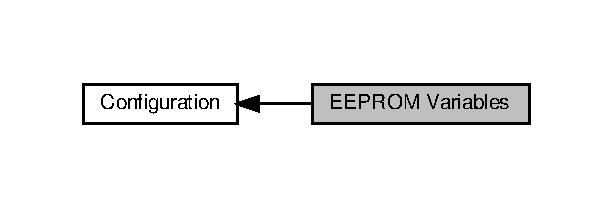
\includegraphics[width=294pt]{group__defines__eeprom__variables}
\end{center}
\end{figure}
\subsection*{Macros}
\begin{DoxyCompactItemize}
\item 
\#define \hyperlink{group__defines__eeprom__variables_ga8f38e463d430bf270a1de27b0af7fd58}{E\+E\+P\+R\+O\+M\+\_\+\+R\+E\+S\+E\+T\+\_\+\+V\+A\+L\+UE}~0x\+FF
\item 
\#define \hyperlink{group__defines__eeprom__variables_ga7780f2cb8d674288b763835a3e81131a}{E\+E\+P\+R\+O\+M\+\_\+\+F\+I\+R\+S\+T\+\_\+\+R\+UN}~0
\item 
\#define \hyperlink{group__defines__eeprom__variables_ga51cfc165574fa74c6e372080bd3fa2f7}{E\+E\+P\+R\+O\+M\+\_\+\+C\+O\+N\+S\+E\+C\+U\+T\+I\+V\+E\+\_\+\+R\+UN}~1
\end{DoxyCompactItemize}


\subsection{Detailed Description}
\begin{DoxyRefDesc}{Test}
\item[\hyperlink{test__test000021}{Test}](ID C\+O\+N\+F\+\_\+\+E\+E\+P\+R\+O\+M\+\_\+\+V\+A\+R\+\_\+\+T0) (S\+EV 1) Check that the E\+E\+P\+R\+O\+M\+\_\+\+R\+E\+S\+E\+T\+\_\+\+V\+A\+L\+UE is suitable. 

(ID C\+O\+N\+F\+\_\+\+E\+E\+P\+R\+O\+M\+\_\+\+V\+A\+R\+\_\+\+T1) (S\+EV 1) Check that the E\+E\+P\+R\+O\+M\+\_\+\+F\+I\+R\+S\+T\+\_\+\+R\+UN is suitable. 

(ID C\+O\+N\+F\+\_\+\+E\+E\+P\+R\+O\+M\+\_\+\+V\+A\+R\+\_\+\+T3) (S\+EV 1) Check that the E\+E\+P\+R\+O\+M\+\_\+\+C\+O\+N\+S\+E\+C\+U\+T\+I\+V\+E\+\_\+\+R\+UN is suitable.\end{DoxyRefDesc}


\subsection{Macro Definition Documentation}
\mbox{\Hypertarget{group__defines__eeprom__variables_ga51cfc165574fa74c6e372080bd3fa2f7}\label{group__defines__eeprom__variables_ga51cfc165574fa74c6e372080bd3fa2f7}} 
\index{E\+E\+P\+R\+O\+M Variables@{E\+E\+P\+R\+O\+M Variables}!E\+E\+P\+R\+O\+M\+\_\+\+C\+O\+N\+S\+E\+C\+U\+T\+I\+V\+E\+\_\+\+R\+UN@{E\+E\+P\+R\+O\+M\+\_\+\+C\+O\+N\+S\+E\+C\+U\+T\+I\+V\+E\+\_\+\+R\+UN}}
\index{E\+E\+P\+R\+O\+M\+\_\+\+C\+O\+N\+S\+E\+C\+U\+T\+I\+V\+E\+\_\+\+R\+UN@{E\+E\+P\+R\+O\+M\+\_\+\+C\+O\+N\+S\+E\+C\+U\+T\+I\+V\+E\+\_\+\+R\+UN}!E\+E\+P\+R\+O\+M Variables@{E\+E\+P\+R\+O\+M Variables}}
\subsubsection{\texorpdfstring{E\+E\+P\+R\+O\+M\+\_\+\+C\+O\+N\+S\+E\+C\+U\+T\+I\+V\+E\+\_\+\+R\+UN}{EEPROM\_CONSECUTIVE\_RUN}}
{\footnotesize\ttfamily \#define E\+E\+P\+R\+O\+M\+\_\+\+C\+O\+N\+S\+E\+C\+U\+T\+I\+V\+E\+\_\+\+R\+UN~1}

The value written to the E\+E\+P\+R\+OM address E\+E\+P\+R\+O\+M\+\_\+\+F\+I\+R\+S\+T\+\_\+\+R\+U\+N\+\_\+\+A\+D\+DR after the first startup sequence. ~\newline
 See \hyperlink{group__defines__eeprom__address__map}{E\+E\+P\+R\+OM Address Map} 

Definition at line 367 of file configuration.\+h.

\mbox{\Hypertarget{group__defines__eeprom__variables_ga7780f2cb8d674288b763835a3e81131a}\label{group__defines__eeprom__variables_ga7780f2cb8d674288b763835a3e81131a}} 
\index{E\+E\+P\+R\+O\+M Variables@{E\+E\+P\+R\+O\+M Variables}!E\+E\+P\+R\+O\+M\+\_\+\+F\+I\+R\+S\+T\+\_\+\+R\+UN@{E\+E\+P\+R\+O\+M\+\_\+\+F\+I\+R\+S\+T\+\_\+\+R\+UN}}
\index{E\+E\+P\+R\+O\+M\+\_\+\+F\+I\+R\+S\+T\+\_\+\+R\+UN@{E\+E\+P\+R\+O\+M\+\_\+\+F\+I\+R\+S\+T\+\_\+\+R\+UN}!E\+E\+P\+R\+O\+M Variables@{E\+E\+P\+R\+O\+M Variables}}
\subsubsection{\texorpdfstring{E\+E\+P\+R\+O\+M\+\_\+\+F\+I\+R\+S\+T\+\_\+\+R\+UN}{EEPROM\_FIRST\_RUN}}
{\footnotesize\ttfamily \#define E\+E\+P\+R\+O\+M\+\_\+\+F\+I\+R\+S\+T\+\_\+\+R\+UN~0}

The value written to the E\+E\+P\+R\+OM address E\+E\+P\+R\+O\+M\+\_\+\+F\+I\+R\+S\+T\+\_\+\+R\+U\+N\+\_\+\+A\+D\+DR before the startup sequence. ~\newline
 See \hyperlink{group__defines__eeprom__address__map}{E\+E\+P\+R\+OM Address Map} 

Definition at line 366 of file configuration.\+h.

\mbox{\Hypertarget{group__defines__eeprom__variables_ga8f38e463d430bf270a1de27b0af7fd58}\label{group__defines__eeprom__variables_ga8f38e463d430bf270a1de27b0af7fd58}} 
\index{E\+E\+P\+R\+O\+M Variables@{E\+E\+P\+R\+O\+M Variables}!E\+E\+P\+R\+O\+M\+\_\+\+R\+E\+S\+E\+T\+\_\+\+V\+A\+L\+UE@{E\+E\+P\+R\+O\+M\+\_\+\+R\+E\+S\+E\+T\+\_\+\+V\+A\+L\+UE}}
\index{E\+E\+P\+R\+O\+M\+\_\+\+R\+E\+S\+E\+T\+\_\+\+V\+A\+L\+UE@{E\+E\+P\+R\+O\+M\+\_\+\+R\+E\+S\+E\+T\+\_\+\+V\+A\+L\+UE}!E\+E\+P\+R\+O\+M Variables@{E\+E\+P\+R\+O\+M Variables}}
\subsubsection{\texorpdfstring{E\+E\+P\+R\+O\+M\+\_\+\+R\+E\+S\+E\+T\+\_\+\+V\+A\+L\+UE}{EEPROM\_RESET\_VALUE}}
{\footnotesize\ttfamily \#define E\+E\+P\+R\+O\+M\+\_\+\+R\+E\+S\+E\+T\+\_\+\+V\+A\+L\+UE~0x\+FF}

E\+E\+P\+R\+OM reset value (255). 

Definition at line 365 of file configuration.\+h.


\hypertarget{group__defines__pin__map}{}\section{Pin Map}
\label{group__defines__pin__map}\index{Pin Map@{Pin Map}}


\tabulinesep=1mm
\begin{longtabu} spread 0pt [c]{*{5}{|X[-1]}|}
\hline
\rowcolor{\tableheadbgcolor}\textbf{ Description}&\textbf{ Arduino core pin}&\textbf{ Physical pin}&\textbf{ Mode}&\textbf{ Direction  }\\\cline{1-5}
\endfirsthead
\hline
\endfoot
\hline
\rowcolor{\tableheadbgcolor}\textbf{ Description}&\textbf{ Arduino core pin}&\textbf{ Physical pin}&\textbf{ Mode}&\textbf{ Direction  }\\\cline{1-5}
\endhead
Solar Cell A Voltage.&A0&P\+C0&A\+N\+A\+L\+OG&IN \\\cline{1-5}
Solar Cell B Voltage.&A7&A\+D\+C7&A\+N\+A\+L\+OG&IN \\\cline{1-5}
Solar Cell C Voltage.&A2&P\+C2&A\+N\+A\+L\+OG&IN \\\cline{1-5}
Analog source for the random number generator (should be left floating).&A6&A\+D\+C6&A\+N\+A\+L\+OG&IN \\\cline{1-5}
M\+P\+PT power control pin.&10&P\+B2&D\+I\+G\+I\+T\+AL&O\+UT \\\cline{1-5}
Deployment mosfet number 1 (controls nicrome wires).&9&P\+B2&D\+I\+G\+I\+T\+AL&O\+UT \\\cline{1-5}
Deployment mosfet number 2 (controls nicrome wires).&8&P\+B0&D\+I\+G\+I\+T\+AL&O\+UT \\\cline{1-5}
Watchdog signal pin.&4&P\+D4&D\+I\+G\+I\+T\+AL&O\+UT \\\cline{1-5}
Radio chip select.&7&P\+D7&D\+I\+G\+I\+T\+AL&O\+UT \\\cline{1-5}
Radio digital pin 1 for reading direct data.&2&P\+D2&D\+I\+G\+I\+T\+AL&IN \\\cline{1-5}
Radio B\+U\+SY pin.&6&P\+D6&D\+I\+G\+I\+T\+AL&IN \\\cline{1-5}
Radio N\+R\+ST pin.&NC&N/A&N/A&N/A \\\cline{1-5}
\end{longtabu}
 


Collaboration diagram for Pin Map\+:
\nopagebreak
\begin{figure}[H]
\begin{center}
\leavevmode
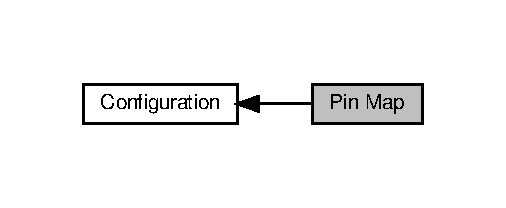
\includegraphics[width=243pt]{group__defines__pin__map}
\end{center}
\end{figure}
\subsection*{Macros}
\begin{DoxyCompactItemize}
\item 
\#define \hyperlink{group__defines__pin__map_gaab66db65014df66541ac9eaa673ca3a2}{A\+N\+A\+L\+O\+G\+\_\+\+I\+N\+\_\+\+S\+O\+L\+A\+R\+\_\+\+A\+\_\+\+V\+O\+L\+T\+A\+G\+E\+\_\+\+P\+IN}~A0
\item 
\#define \hyperlink{group__defines__pin__map_ga8c7edf17cc2aeb690516a5a191a4f3fc}{A\+N\+A\+L\+O\+G\+\_\+\+I\+N\+\_\+\+S\+O\+L\+A\+R\+\_\+\+B\+\_\+\+V\+O\+L\+T\+A\+G\+E\+\_\+\+P\+IN}~A7
\item 
\#define \hyperlink{group__defines__pin__map_ga0810e1baf8fee374bd20c12df8035bb3}{A\+N\+A\+L\+O\+G\+\_\+\+I\+N\+\_\+\+S\+O\+L\+A\+R\+\_\+\+C\+\_\+\+V\+O\+L\+T\+A\+G\+E\+\_\+\+P\+IN}~A2
\item 
\#define \hyperlink{group__defines__pin__map_ga2c37472ba18c707ade2c29026d3ae381}{A\+N\+A\+L\+O\+G\+\_\+\+I\+N\+\_\+\+R\+A\+N\+D\+O\+M\+\_\+\+S\+E\+ED}~A6
\item 
\#define \hyperlink{group__defines__pin__map_ga86d0364d62209e854ee7dc783255e2fe}{D\+I\+G\+I\+T\+A\+L\+\_\+\+O\+U\+T\+\_\+\+M\+P\+P\+T\+\_\+\+P\+IN}~5
\item 
\#define \hyperlink{group__defines__pin__map_gaf1e5e3b5dc8bce89eaae616ec0549f57}{D\+I\+G\+I\+T\+A\+L\+\_\+\+O\+U\+T\+\_\+\+M\+O\+S\+F\+E\+T\+\_\+1}~9
\item 
\#define \hyperlink{group__defines__pin__map_ga8ca8e1d48d4ef0197942b0595a418691}{D\+I\+G\+I\+T\+A\+L\+\_\+\+O\+U\+T\+\_\+\+M\+O\+S\+F\+E\+T\+\_\+2}~8
\item 
\#define \hyperlink{group__defines__pin__map_ga69f1b8867057ee6b56bdcb0263a0d862}{D\+I\+G\+I\+T\+A\+L\+\_\+\+O\+U\+T\+\_\+\+W\+A\+T\+C\+H\+D\+O\+G\+\_\+\+H\+E\+A\+R\+T\+B\+E\+AT}~4
\item 
\#define \hyperlink{group__defines__pin__map_gaecada0a0e3aa3c8f32ce02c1c55e2479}{R\+A\+D\+I\+O\+\_\+\+N\+SS}~7
\item 
\#define \hyperlink{group__defines__pin__map_gac9a997955646825175329d152f768687}{R\+A\+D\+I\+O\+\_\+\+D\+I\+O1}~2
\item 
\#define \hyperlink{group__defines__pin__map_gaffafa27b50d931e6ffbe8e0622ac9658}{R\+A\+D\+I\+O\+\_\+\+B\+U\+SY}~6
\item 
\#define \hyperlink{group__defines__pin__map_ga3cc20f8473f1a75e9957b05d5e220e36}{R\+A\+D\+I\+O\+\_\+\+N\+R\+ST}~R\+A\+D\+I\+O\+L\+I\+B\+\_\+\+NC
\end{DoxyCompactItemize}


\subsection{Detailed Description}
\tabulinesep=1mm
\begin{longtabu} spread 0pt [c]{*{5}{|X[-1]}|}
\hline
\rowcolor{\tableheadbgcolor}\textbf{ Description}&\textbf{ Arduino core pin}&\textbf{ Physical pin}&\textbf{ Mode}&\textbf{ Direction  }\\\cline{1-5}
\endfirsthead
\hline
\endfoot
\hline
\rowcolor{\tableheadbgcolor}\textbf{ Description}&\textbf{ Arduino core pin}&\textbf{ Physical pin}&\textbf{ Mode}&\textbf{ Direction  }\\\cline{1-5}
\endhead
Solar Cell A Voltage.&A0&P\+C0&A\+N\+A\+L\+OG&IN \\\cline{1-5}
Solar Cell B Voltage.&A7&A\+D\+C7&A\+N\+A\+L\+OG&IN \\\cline{1-5}
Solar Cell C Voltage.&A2&P\+C2&A\+N\+A\+L\+OG&IN \\\cline{1-5}
Analog source for the random number generator (should be left floating).&A6&A\+D\+C6&A\+N\+A\+L\+OG&IN \\\cline{1-5}
M\+P\+PT power control pin.&10&P\+B2&D\+I\+G\+I\+T\+AL&O\+UT \\\cline{1-5}
Deployment mosfet number 1 (controls nicrome wires).&9&P\+B2&D\+I\+G\+I\+T\+AL&O\+UT \\\cline{1-5}
Deployment mosfet number 2 (controls nicrome wires).&8&P\+B0&D\+I\+G\+I\+T\+AL&O\+UT \\\cline{1-5}
Watchdog signal pin.&4&P\+D4&D\+I\+G\+I\+T\+AL&O\+UT \\\cline{1-5}
Radio chip select.&7&P\+D7&D\+I\+G\+I\+T\+AL&O\+UT \\\cline{1-5}
Radio digital pin 1 for reading direct data.&2&P\+D2&D\+I\+G\+I\+T\+AL&IN \\\cline{1-5}
Radio B\+U\+SY pin.&6&P\+D6&D\+I\+G\+I\+T\+AL&IN \\\cline{1-5}
Radio N\+R\+ST pin.&NC&N/A&N/A&N/A \\\cline{1-5}
\end{longtabu}


\begin{DoxyRefDesc}{Todo}
\item[\hyperlink{todo__todo000002}{Todo}]Julian -\/$>$ Please check M\+P\+PT pin, seems to be connected to P\+D5 on some versions.\end{DoxyRefDesc}


\begin{DoxyRefDesc}{Test}
\item[\hyperlink{test__test000022}{Test}](ID C\+O\+N\+F\+\_\+\+P\+I\+N\+\_\+\+M\+A\+P\+\_\+\+T0) (S\+EV 1) Check that solar panel A voltage can be read from A\+N\+A\+L\+O\+G\+\_\+\+I\+N\+\_\+\+S\+O\+L\+A\+R\+\_\+\+A\+\_\+\+V\+O\+L\+T\+A\+G\+E\+\_\+\+P\+IN. 

(ID C\+O\+N\+F\+\_\+\+P\+I\+N\+\_\+\+M\+A\+P\+\_\+\+T1) (S\+EV 1) Check that solar panel B voltage can be read from A\+N\+A\+L\+O\+G\+\_\+\+I\+N\+\_\+\+S\+O\+L\+A\+R\+\_\+\+B\+\_\+\+V\+O\+L\+T\+A\+G\+E\+\_\+\+P\+IN. 

(ID C\+O\+N\+F\+\_\+\+P\+I\+N\+\_\+\+M\+A\+P\+\_\+\+T2) (S\+EV 1) Check that solar panel C voltage can be read from A\+N\+A\+L\+O\+G\+\_\+\+I\+N\+\_\+\+S\+O\+L\+A\+R\+\_\+\+C\+\_\+\+V\+O\+L\+T\+A\+G\+E\+\_\+\+P\+IN. 

(ID C\+O\+N\+F\+\_\+\+P\+I\+N\+\_\+\+M\+A\+P\+\_\+\+T3) (S\+EV 1) Check that the random seed analog pin is suitable from A\+N\+A\+L\+O\+G\+\_\+\+I\+N\+\_\+\+R\+A\+N\+D\+O\+M\+\_\+\+S\+E\+ED. 

(ID C\+O\+N\+F\+\_\+\+P\+I\+N\+\_\+\+M\+A\+P\+\_\+\+T4) (S\+EV 1) Check that the M\+P\+PT circuit is controlled correctly using D\+I\+G\+I\+T\+A\+L\+\_\+\+O\+U\+T\+\_\+\+M\+P\+P\+T\+\_\+\+P\+IN. 

(ID C\+O\+N\+F\+\_\+\+P\+I\+N\+\_\+\+M\+A\+P\+\_\+\+T5) (S\+EV 1) Check that the deployment hardware deploys when D\+I\+G\+I\+T\+A\+L\+\_\+\+O\+U\+T\+\_\+\+M\+O\+S\+F\+E\+T\+\_\+1 and D\+I\+G\+I\+T\+A\+L\+\_\+\+O\+U\+T\+\_\+\+M\+O\+S\+F\+E\+T\+\_\+2 are brought high. 

(ID C\+O\+N\+F\+\_\+\+P\+I\+N\+\_\+\+M\+A\+P\+\_\+\+T6) (S\+EV 1) Check that the radio can be communicated with using pins R\+A\+D\+I\+O\+\_\+\+N\+SS, R\+A\+D\+I\+O\+\_\+\+D\+I\+O1, R\+A\+D\+I\+O\+\_\+\+B\+U\+SY and R\+A\+D\+I\+O\+\_\+\+N\+R\+ST.\end{DoxyRefDesc}


\subsection{Macro Definition Documentation}
\mbox{\Hypertarget{group__defines__pin__map_ga2c37472ba18c707ade2c29026d3ae381}\label{group__defines__pin__map_ga2c37472ba18c707ade2c29026d3ae381}} 
\index{Pin Map@{Pin Map}!A\+N\+A\+L\+O\+G\+\_\+\+I\+N\+\_\+\+R\+A\+N\+D\+O\+M\+\_\+\+S\+E\+ED@{A\+N\+A\+L\+O\+G\+\_\+\+I\+N\+\_\+\+R\+A\+N\+D\+O\+M\+\_\+\+S\+E\+ED}}
\index{A\+N\+A\+L\+O\+G\+\_\+\+I\+N\+\_\+\+R\+A\+N\+D\+O\+M\+\_\+\+S\+E\+ED@{A\+N\+A\+L\+O\+G\+\_\+\+I\+N\+\_\+\+R\+A\+N\+D\+O\+M\+\_\+\+S\+E\+ED}!Pin Map@{Pin Map}}
\subsubsection{\texorpdfstring{A\+N\+A\+L\+O\+G\+\_\+\+I\+N\+\_\+\+R\+A\+N\+D\+O\+M\+\_\+\+S\+E\+ED}{ANALOG\_IN\_RANDOM\_SEED}}
{\footnotesize\ttfamily \#define A\+N\+A\+L\+O\+G\+\_\+\+I\+N\+\_\+\+R\+A\+N\+D\+O\+M\+\_\+\+S\+E\+ED~A6}

A\+D\+C6; used as source for random\+Seed(), should be left floating 

Definition at line 407 of file configuration.\+h.

\mbox{\Hypertarget{group__defines__pin__map_gaab66db65014df66541ac9eaa673ca3a2}\label{group__defines__pin__map_gaab66db65014df66541ac9eaa673ca3a2}} 
\index{Pin Map@{Pin Map}!A\+N\+A\+L\+O\+G\+\_\+\+I\+N\+\_\+\+S\+O\+L\+A\+R\+\_\+\+A\+\_\+\+V\+O\+L\+T\+A\+G\+E\+\_\+\+P\+IN@{A\+N\+A\+L\+O\+G\+\_\+\+I\+N\+\_\+\+S\+O\+L\+A\+R\+\_\+\+A\+\_\+\+V\+O\+L\+T\+A\+G\+E\+\_\+\+P\+IN}}
\index{A\+N\+A\+L\+O\+G\+\_\+\+I\+N\+\_\+\+S\+O\+L\+A\+R\+\_\+\+A\+\_\+\+V\+O\+L\+T\+A\+G\+E\+\_\+\+P\+IN@{A\+N\+A\+L\+O\+G\+\_\+\+I\+N\+\_\+\+S\+O\+L\+A\+R\+\_\+\+A\+\_\+\+V\+O\+L\+T\+A\+G\+E\+\_\+\+P\+IN}!Pin Map@{Pin Map}}
\subsubsection{\texorpdfstring{A\+N\+A\+L\+O\+G\+\_\+\+I\+N\+\_\+\+S\+O\+L\+A\+R\+\_\+\+A\+\_\+\+V\+O\+L\+T\+A\+G\+E\+\_\+\+P\+IN}{ANALOG\_IN\_SOLAR\_A\_VOLTAGE\_PIN}}
{\footnotesize\ttfamily \#define A\+N\+A\+L\+O\+G\+\_\+\+I\+N\+\_\+\+S\+O\+L\+A\+R\+\_\+\+A\+\_\+\+V\+O\+L\+T\+A\+G\+E\+\_\+\+P\+IN~A0}

P\+C0 

Definition at line 404 of file configuration.\+h.

\mbox{\Hypertarget{group__defines__pin__map_ga8c7edf17cc2aeb690516a5a191a4f3fc}\label{group__defines__pin__map_ga8c7edf17cc2aeb690516a5a191a4f3fc}} 
\index{Pin Map@{Pin Map}!A\+N\+A\+L\+O\+G\+\_\+\+I\+N\+\_\+\+S\+O\+L\+A\+R\+\_\+\+B\+\_\+\+V\+O\+L\+T\+A\+G\+E\+\_\+\+P\+IN@{A\+N\+A\+L\+O\+G\+\_\+\+I\+N\+\_\+\+S\+O\+L\+A\+R\+\_\+\+B\+\_\+\+V\+O\+L\+T\+A\+G\+E\+\_\+\+P\+IN}}
\index{A\+N\+A\+L\+O\+G\+\_\+\+I\+N\+\_\+\+S\+O\+L\+A\+R\+\_\+\+B\+\_\+\+V\+O\+L\+T\+A\+G\+E\+\_\+\+P\+IN@{A\+N\+A\+L\+O\+G\+\_\+\+I\+N\+\_\+\+S\+O\+L\+A\+R\+\_\+\+B\+\_\+\+V\+O\+L\+T\+A\+G\+E\+\_\+\+P\+IN}!Pin Map@{Pin Map}}
\subsubsection{\texorpdfstring{A\+N\+A\+L\+O\+G\+\_\+\+I\+N\+\_\+\+S\+O\+L\+A\+R\+\_\+\+B\+\_\+\+V\+O\+L\+T\+A\+G\+E\+\_\+\+P\+IN}{ANALOG\_IN\_SOLAR\_B\_VOLTAGE\_PIN}}
{\footnotesize\ttfamily \#define A\+N\+A\+L\+O\+G\+\_\+\+I\+N\+\_\+\+S\+O\+L\+A\+R\+\_\+\+B\+\_\+\+V\+O\+L\+T\+A\+G\+E\+\_\+\+P\+IN~A7}

A\+D\+C7 

Definition at line 405 of file configuration.\+h.

\mbox{\Hypertarget{group__defines__pin__map_ga0810e1baf8fee374bd20c12df8035bb3}\label{group__defines__pin__map_ga0810e1baf8fee374bd20c12df8035bb3}} 
\index{Pin Map@{Pin Map}!A\+N\+A\+L\+O\+G\+\_\+\+I\+N\+\_\+\+S\+O\+L\+A\+R\+\_\+\+C\+\_\+\+V\+O\+L\+T\+A\+G\+E\+\_\+\+P\+IN@{A\+N\+A\+L\+O\+G\+\_\+\+I\+N\+\_\+\+S\+O\+L\+A\+R\+\_\+\+C\+\_\+\+V\+O\+L\+T\+A\+G\+E\+\_\+\+P\+IN}}
\index{A\+N\+A\+L\+O\+G\+\_\+\+I\+N\+\_\+\+S\+O\+L\+A\+R\+\_\+\+C\+\_\+\+V\+O\+L\+T\+A\+G\+E\+\_\+\+P\+IN@{A\+N\+A\+L\+O\+G\+\_\+\+I\+N\+\_\+\+S\+O\+L\+A\+R\+\_\+\+C\+\_\+\+V\+O\+L\+T\+A\+G\+E\+\_\+\+P\+IN}!Pin Map@{Pin Map}}
\subsubsection{\texorpdfstring{A\+N\+A\+L\+O\+G\+\_\+\+I\+N\+\_\+\+S\+O\+L\+A\+R\+\_\+\+C\+\_\+\+V\+O\+L\+T\+A\+G\+E\+\_\+\+P\+IN}{ANALOG\_IN\_SOLAR\_C\_VOLTAGE\_PIN}}
{\footnotesize\ttfamily \#define A\+N\+A\+L\+O\+G\+\_\+\+I\+N\+\_\+\+S\+O\+L\+A\+R\+\_\+\+C\+\_\+\+V\+O\+L\+T\+A\+G\+E\+\_\+\+P\+IN~A2}

P\+C2 

Definition at line 406 of file configuration.\+h.

\mbox{\Hypertarget{group__defines__pin__map_gaf1e5e3b5dc8bce89eaae616ec0549f57}\label{group__defines__pin__map_gaf1e5e3b5dc8bce89eaae616ec0549f57}} 
\index{Pin Map@{Pin Map}!D\+I\+G\+I\+T\+A\+L\+\_\+\+O\+U\+T\+\_\+\+M\+O\+S\+F\+E\+T\+\_\+1@{D\+I\+G\+I\+T\+A\+L\+\_\+\+O\+U\+T\+\_\+\+M\+O\+S\+F\+E\+T\+\_\+1}}
\index{D\+I\+G\+I\+T\+A\+L\+\_\+\+O\+U\+T\+\_\+\+M\+O\+S\+F\+E\+T\+\_\+1@{D\+I\+G\+I\+T\+A\+L\+\_\+\+O\+U\+T\+\_\+\+M\+O\+S\+F\+E\+T\+\_\+1}!Pin Map@{Pin Map}}
\subsubsection{\texorpdfstring{D\+I\+G\+I\+T\+A\+L\+\_\+\+O\+U\+T\+\_\+\+M\+O\+S\+F\+E\+T\+\_\+1}{DIGITAL\_OUT\_MOSFET\_1}}
{\footnotesize\ttfamily \#define D\+I\+G\+I\+T\+A\+L\+\_\+\+O\+U\+T\+\_\+\+M\+O\+S\+F\+E\+T\+\_\+1~9}

P\+B1 

Definition at line 409 of file configuration.\+h.

\mbox{\Hypertarget{group__defines__pin__map_ga8ca8e1d48d4ef0197942b0595a418691}\label{group__defines__pin__map_ga8ca8e1d48d4ef0197942b0595a418691}} 
\index{Pin Map@{Pin Map}!D\+I\+G\+I\+T\+A\+L\+\_\+\+O\+U\+T\+\_\+\+M\+O\+S\+F\+E\+T\+\_\+2@{D\+I\+G\+I\+T\+A\+L\+\_\+\+O\+U\+T\+\_\+\+M\+O\+S\+F\+E\+T\+\_\+2}}
\index{D\+I\+G\+I\+T\+A\+L\+\_\+\+O\+U\+T\+\_\+\+M\+O\+S\+F\+E\+T\+\_\+2@{D\+I\+G\+I\+T\+A\+L\+\_\+\+O\+U\+T\+\_\+\+M\+O\+S\+F\+E\+T\+\_\+2}!Pin Map@{Pin Map}}
\subsubsection{\texorpdfstring{D\+I\+G\+I\+T\+A\+L\+\_\+\+O\+U\+T\+\_\+\+M\+O\+S\+F\+E\+T\+\_\+2}{DIGITAL\_OUT\_MOSFET\_2}}
{\footnotesize\ttfamily \#define D\+I\+G\+I\+T\+A\+L\+\_\+\+O\+U\+T\+\_\+\+M\+O\+S\+F\+E\+T\+\_\+2~8}

P\+B0 

Definition at line 410 of file configuration.\+h.

\mbox{\Hypertarget{group__defines__pin__map_ga86d0364d62209e854ee7dc783255e2fe}\label{group__defines__pin__map_ga86d0364d62209e854ee7dc783255e2fe}} 
\index{Pin Map@{Pin Map}!D\+I\+G\+I\+T\+A\+L\+\_\+\+O\+U\+T\+\_\+\+M\+P\+P\+T\+\_\+\+P\+IN@{D\+I\+G\+I\+T\+A\+L\+\_\+\+O\+U\+T\+\_\+\+M\+P\+P\+T\+\_\+\+P\+IN}}
\index{D\+I\+G\+I\+T\+A\+L\+\_\+\+O\+U\+T\+\_\+\+M\+P\+P\+T\+\_\+\+P\+IN@{D\+I\+G\+I\+T\+A\+L\+\_\+\+O\+U\+T\+\_\+\+M\+P\+P\+T\+\_\+\+P\+IN}!Pin Map@{Pin Map}}
\subsubsection{\texorpdfstring{D\+I\+G\+I\+T\+A\+L\+\_\+\+O\+U\+T\+\_\+\+M\+P\+P\+T\+\_\+\+P\+IN}{DIGITAL\_OUT\_MPPT\_PIN}}
{\footnotesize\ttfamily \#define D\+I\+G\+I\+T\+A\+L\+\_\+\+O\+U\+T\+\_\+\+M\+P\+P\+T\+\_\+\+P\+IN~5}

P\+B2 

Definition at line 408 of file configuration.\+h.

\mbox{\Hypertarget{group__defines__pin__map_ga69f1b8867057ee6b56bdcb0263a0d862}\label{group__defines__pin__map_ga69f1b8867057ee6b56bdcb0263a0d862}} 
\index{Pin Map@{Pin Map}!D\+I\+G\+I\+T\+A\+L\+\_\+\+O\+U\+T\+\_\+\+W\+A\+T\+C\+H\+D\+O\+G\+\_\+\+H\+E\+A\+R\+T\+B\+E\+AT@{D\+I\+G\+I\+T\+A\+L\+\_\+\+O\+U\+T\+\_\+\+W\+A\+T\+C\+H\+D\+O\+G\+\_\+\+H\+E\+A\+R\+T\+B\+E\+AT}}
\index{D\+I\+G\+I\+T\+A\+L\+\_\+\+O\+U\+T\+\_\+\+W\+A\+T\+C\+H\+D\+O\+G\+\_\+\+H\+E\+A\+R\+T\+B\+E\+AT@{D\+I\+G\+I\+T\+A\+L\+\_\+\+O\+U\+T\+\_\+\+W\+A\+T\+C\+H\+D\+O\+G\+\_\+\+H\+E\+A\+R\+T\+B\+E\+AT}!Pin Map@{Pin Map}}
\subsubsection{\texorpdfstring{D\+I\+G\+I\+T\+A\+L\+\_\+\+O\+U\+T\+\_\+\+W\+A\+T\+C\+H\+D\+O\+G\+\_\+\+H\+E\+A\+R\+T\+B\+E\+AT}{DIGITAL\_OUT\_WATCHDOG\_HEARTBEAT}}
{\footnotesize\ttfamily \#define D\+I\+G\+I\+T\+A\+L\+\_\+\+O\+U\+T\+\_\+\+W\+A\+T\+C\+H\+D\+O\+G\+\_\+\+H\+E\+A\+R\+T\+B\+E\+AT~4}

P\+D4 

Definition at line 411 of file configuration.\+h.

\mbox{\Hypertarget{group__defines__pin__map_gaffafa27b50d931e6ffbe8e0622ac9658}\label{group__defines__pin__map_gaffafa27b50d931e6ffbe8e0622ac9658}} 
\index{Pin Map@{Pin Map}!R\+A\+D\+I\+O\+\_\+\+B\+U\+SY@{R\+A\+D\+I\+O\+\_\+\+B\+U\+SY}}
\index{R\+A\+D\+I\+O\+\_\+\+B\+U\+SY@{R\+A\+D\+I\+O\+\_\+\+B\+U\+SY}!Pin Map@{Pin Map}}
\subsubsection{\texorpdfstring{R\+A\+D\+I\+O\+\_\+\+B\+U\+SY}{RADIO\_BUSY}}
{\footnotesize\ttfamily \#define R\+A\+D\+I\+O\+\_\+\+B\+U\+SY~6}

P\+D6 

Definition at line 414 of file configuration.\+h.

\mbox{\Hypertarget{group__defines__pin__map_gac9a997955646825175329d152f768687}\label{group__defines__pin__map_gac9a997955646825175329d152f768687}} 
\index{Pin Map@{Pin Map}!R\+A\+D\+I\+O\+\_\+\+D\+I\+O1@{R\+A\+D\+I\+O\+\_\+\+D\+I\+O1}}
\index{R\+A\+D\+I\+O\+\_\+\+D\+I\+O1@{R\+A\+D\+I\+O\+\_\+\+D\+I\+O1}!Pin Map@{Pin Map}}
\subsubsection{\texorpdfstring{R\+A\+D\+I\+O\+\_\+\+D\+I\+O1}{RADIO\_DIO1}}
{\footnotesize\ttfamily \#define R\+A\+D\+I\+O\+\_\+\+D\+I\+O1~2}

P\+D2 

Definition at line 413 of file configuration.\+h.

\mbox{\Hypertarget{group__defines__pin__map_ga3cc20f8473f1a75e9957b05d5e220e36}\label{group__defines__pin__map_ga3cc20f8473f1a75e9957b05d5e220e36}} 
\index{Pin Map@{Pin Map}!R\+A\+D\+I\+O\+\_\+\+N\+R\+ST@{R\+A\+D\+I\+O\+\_\+\+N\+R\+ST}}
\index{R\+A\+D\+I\+O\+\_\+\+N\+R\+ST@{R\+A\+D\+I\+O\+\_\+\+N\+R\+ST}!Pin Map@{Pin Map}}
\subsubsection{\texorpdfstring{R\+A\+D\+I\+O\+\_\+\+N\+R\+ST}{RADIO\_NRST}}
{\footnotesize\ttfamily \#define R\+A\+D\+I\+O\+\_\+\+N\+R\+ST~R\+A\+D\+I\+O\+L\+I\+B\+\_\+\+NC}

Not connected 

Definition at line 415 of file configuration.\+h.

\mbox{\Hypertarget{group__defines__pin__map_gaecada0a0e3aa3c8f32ce02c1c55e2479}\label{group__defines__pin__map_gaecada0a0e3aa3c8f32ce02c1c55e2479}} 
\index{Pin Map@{Pin Map}!R\+A\+D\+I\+O\+\_\+\+N\+SS@{R\+A\+D\+I\+O\+\_\+\+N\+SS}}
\index{R\+A\+D\+I\+O\+\_\+\+N\+SS@{R\+A\+D\+I\+O\+\_\+\+N\+SS}!Pin Map@{Pin Map}}
\subsubsection{\texorpdfstring{R\+A\+D\+I\+O\+\_\+\+N\+SS}{RADIO\_NSS}}
{\footnotesize\ttfamily \#define R\+A\+D\+I\+O\+\_\+\+N\+SS~7}

P\+D7 

Definition at line 412 of file configuration.\+h.


\hypertarget{group__defines__tmp100__configuration}{}\section{T\+M\+P100 Temperature Sensor Configuration}
\label{group__defines__tmp100__configuration}\index{T\+M\+P100 Temperature Sensor Configuration@{T\+M\+P100 Temperature Sensor Configuration}}
Collaboration diagram for T\+M\+P100 Temperature Sensor Configuration\+:
\nopagebreak
\begin{figure}[H]
\begin{center}
\leavevmode
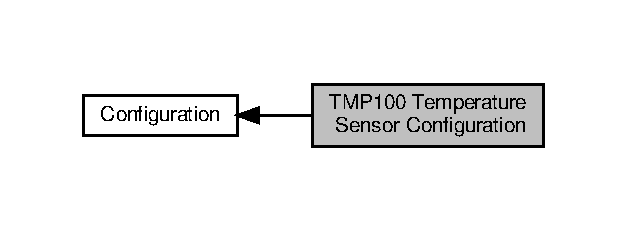
\includegraphics[width=301pt]{group__defines__tmp100__configuration}
\end{center}
\end{figure}
\subsection*{Macros}
\begin{DoxyCompactItemize}
\item 
\#define \hyperlink{group__defines__tmp100__configuration_gaa038d9fe5bc1bccc19789a7a958065f6}{B\+O\+A\+R\+D\+\_\+\+T\+E\+M\+P\+\_\+\+S\+E\+N\+S\+O\+R\+\_\+\+A\+D\+DR}~0b1001100
\item 
\#define \hyperlink{group__defines__tmp100__configuration_gacdbd26cf9028150bbe6cb0734e4d7674}{B\+A\+T\+T\+E\+R\+Y\+\_\+\+T\+E\+M\+P\+\_\+\+S\+E\+N\+S\+O\+R\+\_\+\+A\+D\+DR}~0b1001011
\item 
\#define \hyperlink{group__defines__tmp100__configuration_ga32a821ac31cd3f35b29eeaedd2ada8a7}{T\+E\+M\+P\+\_\+\+S\+E\+N\+S\+O\+R\+\_\+\+R\+E\+G\+\_\+\+C\+O\+N\+F\+IG}~0b01
\item 
\#define \hyperlink{group__defines__tmp100__configuration_ga3d36edb45de9609b03bd822d6c918112}{T\+E\+M\+P\+\_\+\+S\+E\+N\+S\+O\+R\+\_\+\+R\+E\+S\+O\+L\+U\+T\+I\+O\+N\+\_\+9\+\_\+\+B\+I\+TS}~0b00000000
\item 
\#define \hyperlink{group__defines__tmp100__configuration_gaf70d4e6a476885b74766b5df9a3fbc09}{T\+E\+M\+P\+\_\+\+S\+E\+N\+S\+O\+R\+\_\+\+R\+E\+S\+O\+L\+U\+T\+I\+O\+N\+\_\+10\+\_\+\+B\+I\+TS}~0b00100000
\item 
\#define \hyperlink{group__defines__tmp100__configuration_gac97175df8d77fc1235d887430fbb1dd3}{T\+E\+M\+P\+\_\+\+S\+E\+N\+S\+O\+R\+\_\+\+R\+E\+S\+O\+L\+U\+T\+I\+O\+N\+\_\+11\+\_\+\+B\+I\+TS}~0b01000000
\item 
\#define \hyperlink{group__defines__tmp100__configuration_ga5e14ff4c60e05aec1827aa1ecb1db92b}{T\+E\+M\+P\+\_\+\+S\+E\+N\+S\+O\+R\+\_\+\+R\+E\+S\+O\+L\+U\+T\+I\+O\+N\+\_\+12\+\_\+\+B\+I\+TS}~0b01100000
\end{DoxyCompactItemize}


\subsection{Detailed Description}
\begin{DoxyRefDesc}{Test}
\item[\hyperlink{test__test000023}{Test}](ID C\+O\+N\+F\+\_\+\+T\+M\+P100\+\_\+\+T0) (S\+EV 1) Check that the T\+M\+P100 sensor returns the correct value (given the resolution) from the Wire connection.\end{DoxyRefDesc}


\subsection{Macro Definition Documentation}
\mbox{\Hypertarget{group__defines__tmp100__configuration_gacdbd26cf9028150bbe6cb0734e4d7674}\label{group__defines__tmp100__configuration_gacdbd26cf9028150bbe6cb0734e4d7674}} 
\index{T\+M\+P100 Temperature Sensor Configuration@{T\+M\+P100 Temperature Sensor Configuration}!B\+A\+T\+T\+E\+R\+Y\+\_\+\+T\+E\+M\+P\+\_\+\+S\+E\+N\+S\+O\+R\+\_\+\+A\+D\+DR@{B\+A\+T\+T\+E\+R\+Y\+\_\+\+T\+E\+M\+P\+\_\+\+S\+E\+N\+S\+O\+R\+\_\+\+A\+D\+DR}}
\index{B\+A\+T\+T\+E\+R\+Y\+\_\+\+T\+E\+M\+P\+\_\+\+S\+E\+N\+S\+O\+R\+\_\+\+A\+D\+DR@{B\+A\+T\+T\+E\+R\+Y\+\_\+\+T\+E\+M\+P\+\_\+\+S\+E\+N\+S\+O\+R\+\_\+\+A\+D\+DR}!T\+M\+P100 Temperature Sensor Configuration@{T\+M\+P100 Temperature Sensor Configuration}}
\subsubsection{\texorpdfstring{B\+A\+T\+T\+E\+R\+Y\+\_\+\+T\+E\+M\+P\+\_\+\+S\+E\+N\+S\+O\+R\+\_\+\+A\+D\+DR}{BATTERY\_TEMP\_SENSOR\_ADDR}}
{\footnotesize\ttfamily \#define B\+A\+T\+T\+E\+R\+Y\+\_\+\+T\+E\+M\+P\+\_\+\+S\+E\+N\+S\+O\+R\+\_\+\+A\+D\+DR~0b1001011}

Battery T\+M\+P100 temperature sensor Wire address. 

Definition at line 428 of file configuration.\+h.

\mbox{\Hypertarget{group__defines__tmp100__configuration_gaa038d9fe5bc1bccc19789a7a958065f6}\label{group__defines__tmp100__configuration_gaa038d9fe5bc1bccc19789a7a958065f6}} 
\index{T\+M\+P100 Temperature Sensor Configuration@{T\+M\+P100 Temperature Sensor Configuration}!B\+O\+A\+R\+D\+\_\+\+T\+E\+M\+P\+\_\+\+S\+E\+N\+S\+O\+R\+\_\+\+A\+D\+DR@{B\+O\+A\+R\+D\+\_\+\+T\+E\+M\+P\+\_\+\+S\+E\+N\+S\+O\+R\+\_\+\+A\+D\+DR}}
\index{B\+O\+A\+R\+D\+\_\+\+T\+E\+M\+P\+\_\+\+S\+E\+N\+S\+O\+R\+\_\+\+A\+D\+DR@{B\+O\+A\+R\+D\+\_\+\+T\+E\+M\+P\+\_\+\+S\+E\+N\+S\+O\+R\+\_\+\+A\+D\+DR}!T\+M\+P100 Temperature Sensor Configuration@{T\+M\+P100 Temperature Sensor Configuration}}
\subsubsection{\texorpdfstring{B\+O\+A\+R\+D\+\_\+\+T\+E\+M\+P\+\_\+\+S\+E\+N\+S\+O\+R\+\_\+\+A\+D\+DR}{BOARD\_TEMP\_SENSOR\_ADDR}}
{\footnotesize\ttfamily \#define B\+O\+A\+R\+D\+\_\+\+T\+E\+M\+P\+\_\+\+S\+E\+N\+S\+O\+R\+\_\+\+A\+D\+DR~0b1001100}

Board T\+M\+P100 temperature sensor Wire address. 

Definition at line 427 of file configuration.\+h.

\mbox{\Hypertarget{group__defines__tmp100__configuration_ga32a821ac31cd3f35b29eeaedd2ada8a7}\label{group__defines__tmp100__configuration_ga32a821ac31cd3f35b29eeaedd2ada8a7}} 
\index{T\+M\+P100 Temperature Sensor Configuration@{T\+M\+P100 Temperature Sensor Configuration}!T\+E\+M\+P\+\_\+\+S\+E\+N\+S\+O\+R\+\_\+\+R\+E\+G\+\_\+\+C\+O\+N\+F\+IG@{T\+E\+M\+P\+\_\+\+S\+E\+N\+S\+O\+R\+\_\+\+R\+E\+G\+\_\+\+C\+O\+N\+F\+IG}}
\index{T\+E\+M\+P\+\_\+\+S\+E\+N\+S\+O\+R\+\_\+\+R\+E\+G\+\_\+\+C\+O\+N\+F\+IG@{T\+E\+M\+P\+\_\+\+S\+E\+N\+S\+O\+R\+\_\+\+R\+E\+G\+\_\+\+C\+O\+N\+F\+IG}!T\+M\+P100 Temperature Sensor Configuration@{T\+M\+P100 Temperature Sensor Configuration}}
\subsubsection{\texorpdfstring{T\+E\+M\+P\+\_\+\+S\+E\+N\+S\+O\+R\+\_\+\+R\+E\+G\+\_\+\+C\+O\+N\+F\+IG}{TEMP\_SENSOR\_REG\_CONFIG}}
{\footnotesize\ttfamily \#define T\+E\+M\+P\+\_\+\+S\+E\+N\+S\+O\+R\+\_\+\+R\+E\+G\+\_\+\+C\+O\+N\+F\+IG~0b01}

Initial temperature sensor configuration value (1). 

Definition at line 429 of file configuration.\+h.

\mbox{\Hypertarget{group__defines__tmp100__configuration_gaf70d4e6a476885b74766b5df9a3fbc09}\label{group__defines__tmp100__configuration_gaf70d4e6a476885b74766b5df9a3fbc09}} 
\index{T\+M\+P100 Temperature Sensor Configuration@{T\+M\+P100 Temperature Sensor Configuration}!T\+E\+M\+P\+\_\+\+S\+E\+N\+S\+O\+R\+\_\+\+R\+E\+S\+O\+L\+U\+T\+I\+O\+N\+\_\+10\+\_\+\+B\+I\+TS@{T\+E\+M\+P\+\_\+\+S\+E\+N\+S\+O\+R\+\_\+\+R\+E\+S\+O\+L\+U\+T\+I\+O\+N\+\_\+10\+\_\+\+B\+I\+TS}}
\index{T\+E\+M\+P\+\_\+\+S\+E\+N\+S\+O\+R\+\_\+\+R\+E\+S\+O\+L\+U\+T\+I\+O\+N\+\_\+10\+\_\+\+B\+I\+TS@{T\+E\+M\+P\+\_\+\+S\+E\+N\+S\+O\+R\+\_\+\+R\+E\+S\+O\+L\+U\+T\+I\+O\+N\+\_\+10\+\_\+\+B\+I\+TS}!T\+M\+P100 Temperature Sensor Configuration@{T\+M\+P100 Temperature Sensor Configuration}}
\subsubsection{\texorpdfstring{T\+E\+M\+P\+\_\+\+S\+E\+N\+S\+O\+R\+\_\+\+R\+E\+S\+O\+L\+U\+T\+I\+O\+N\+\_\+10\+\_\+\+B\+I\+TS}{TEMP\_SENSOR\_RESOLUTION\_10\_BITS}}
{\footnotesize\ttfamily \#define T\+E\+M\+P\+\_\+\+S\+E\+N\+S\+O\+R\+\_\+\+R\+E\+S\+O\+L\+U\+T\+I\+O\+N\+\_\+10\+\_\+\+B\+I\+TS~0b00100000}

e.\+g. 0.\+25 deg. C 

Definition at line 431 of file configuration.\+h.

\mbox{\Hypertarget{group__defines__tmp100__configuration_gac97175df8d77fc1235d887430fbb1dd3}\label{group__defines__tmp100__configuration_gac97175df8d77fc1235d887430fbb1dd3}} 
\index{T\+M\+P100 Temperature Sensor Configuration@{T\+M\+P100 Temperature Sensor Configuration}!T\+E\+M\+P\+\_\+\+S\+E\+N\+S\+O\+R\+\_\+\+R\+E\+S\+O\+L\+U\+T\+I\+O\+N\+\_\+11\+\_\+\+B\+I\+TS@{T\+E\+M\+P\+\_\+\+S\+E\+N\+S\+O\+R\+\_\+\+R\+E\+S\+O\+L\+U\+T\+I\+O\+N\+\_\+11\+\_\+\+B\+I\+TS}}
\index{T\+E\+M\+P\+\_\+\+S\+E\+N\+S\+O\+R\+\_\+\+R\+E\+S\+O\+L\+U\+T\+I\+O\+N\+\_\+11\+\_\+\+B\+I\+TS@{T\+E\+M\+P\+\_\+\+S\+E\+N\+S\+O\+R\+\_\+\+R\+E\+S\+O\+L\+U\+T\+I\+O\+N\+\_\+11\+\_\+\+B\+I\+TS}!T\+M\+P100 Temperature Sensor Configuration@{T\+M\+P100 Temperature Sensor Configuration}}
\subsubsection{\texorpdfstring{T\+E\+M\+P\+\_\+\+S\+E\+N\+S\+O\+R\+\_\+\+R\+E\+S\+O\+L\+U\+T\+I\+O\+N\+\_\+11\+\_\+\+B\+I\+TS}{TEMP\_SENSOR\_RESOLUTION\_11\_BITS}}
{\footnotesize\ttfamily \#define T\+E\+M\+P\+\_\+\+S\+E\+N\+S\+O\+R\+\_\+\+R\+E\+S\+O\+L\+U\+T\+I\+O\+N\+\_\+11\+\_\+\+B\+I\+TS~0b01000000}

e.\+g. 0.\+125 deg. C 

Definition at line 432 of file configuration.\+h.

\mbox{\Hypertarget{group__defines__tmp100__configuration_ga5e14ff4c60e05aec1827aa1ecb1db92b}\label{group__defines__tmp100__configuration_ga5e14ff4c60e05aec1827aa1ecb1db92b}} 
\index{T\+M\+P100 Temperature Sensor Configuration@{T\+M\+P100 Temperature Sensor Configuration}!T\+E\+M\+P\+\_\+\+S\+E\+N\+S\+O\+R\+\_\+\+R\+E\+S\+O\+L\+U\+T\+I\+O\+N\+\_\+12\+\_\+\+B\+I\+TS@{T\+E\+M\+P\+\_\+\+S\+E\+N\+S\+O\+R\+\_\+\+R\+E\+S\+O\+L\+U\+T\+I\+O\+N\+\_\+12\+\_\+\+B\+I\+TS}}
\index{T\+E\+M\+P\+\_\+\+S\+E\+N\+S\+O\+R\+\_\+\+R\+E\+S\+O\+L\+U\+T\+I\+O\+N\+\_\+12\+\_\+\+B\+I\+TS@{T\+E\+M\+P\+\_\+\+S\+E\+N\+S\+O\+R\+\_\+\+R\+E\+S\+O\+L\+U\+T\+I\+O\+N\+\_\+12\+\_\+\+B\+I\+TS}!T\+M\+P100 Temperature Sensor Configuration@{T\+M\+P100 Temperature Sensor Configuration}}
\subsubsection{\texorpdfstring{T\+E\+M\+P\+\_\+\+S\+E\+N\+S\+O\+R\+\_\+\+R\+E\+S\+O\+L\+U\+T\+I\+O\+N\+\_\+12\+\_\+\+B\+I\+TS}{TEMP\_SENSOR\_RESOLUTION\_12\_BITS}}
{\footnotesize\ttfamily \#define T\+E\+M\+P\+\_\+\+S\+E\+N\+S\+O\+R\+\_\+\+R\+E\+S\+O\+L\+U\+T\+I\+O\+N\+\_\+12\+\_\+\+B\+I\+TS~0b01100000}

e.\+g. 0.\+0625 deg. C 

Definition at line 433 of file configuration.\+h.

\mbox{\Hypertarget{group__defines__tmp100__configuration_ga3d36edb45de9609b03bd822d6c918112}\label{group__defines__tmp100__configuration_ga3d36edb45de9609b03bd822d6c918112}} 
\index{T\+M\+P100 Temperature Sensor Configuration@{T\+M\+P100 Temperature Sensor Configuration}!T\+E\+M\+P\+\_\+\+S\+E\+N\+S\+O\+R\+\_\+\+R\+E\+S\+O\+L\+U\+T\+I\+O\+N\+\_\+9\+\_\+\+B\+I\+TS@{T\+E\+M\+P\+\_\+\+S\+E\+N\+S\+O\+R\+\_\+\+R\+E\+S\+O\+L\+U\+T\+I\+O\+N\+\_\+9\+\_\+\+B\+I\+TS}}
\index{T\+E\+M\+P\+\_\+\+S\+E\+N\+S\+O\+R\+\_\+\+R\+E\+S\+O\+L\+U\+T\+I\+O\+N\+\_\+9\+\_\+\+B\+I\+TS@{T\+E\+M\+P\+\_\+\+S\+E\+N\+S\+O\+R\+\_\+\+R\+E\+S\+O\+L\+U\+T\+I\+O\+N\+\_\+9\+\_\+\+B\+I\+TS}!T\+M\+P100 Temperature Sensor Configuration@{T\+M\+P100 Temperature Sensor Configuration}}
\subsubsection{\texorpdfstring{T\+E\+M\+P\+\_\+\+S\+E\+N\+S\+O\+R\+\_\+\+R\+E\+S\+O\+L\+U\+T\+I\+O\+N\+\_\+9\+\_\+\+B\+I\+TS}{TEMP\_SENSOR\_RESOLUTION\_9\_BITS}}
{\footnotesize\ttfamily \#define T\+E\+M\+P\+\_\+\+S\+E\+N\+S\+O\+R\+\_\+\+R\+E\+S\+O\+L\+U\+T\+I\+O\+N\+\_\+9\+\_\+\+B\+I\+TS~0b00000000}

e.\+g. 0.\+5 deg. C 

Definition at line 430 of file configuration.\+h.


\hypertarget{group__defines__mcu__temperature__configuration}{}\section{M\+CU Temperature Sensor Configuration}
\label{group__defines__mcu__temperature__configuration}\index{M\+C\+U Temperature Sensor Configuration@{M\+C\+U Temperature Sensor Configuration}}
Collaboration diagram for M\+CU Temperature Sensor Configuration\+:
\nopagebreak
\begin{figure}[H]
\begin{center}
\leavevmode
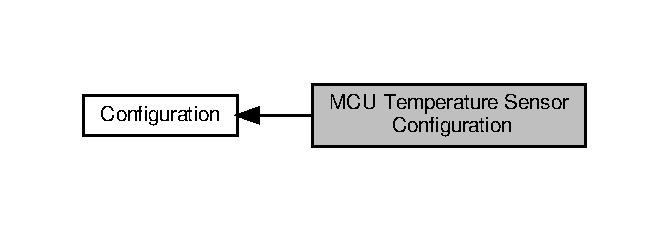
\includegraphics[width=321pt]{group__defines__mcu__temperature__configuration}
\end{center}
\end{figure}
\subsection*{Macros}
\begin{DoxyCompactItemize}
\item 
\#define \hyperlink{group__defines__mcu__temperature__configuration_ga9c0099995bb74deac3678037a53abed3}{M\+C\+U\+\_\+\+T\+E\+M\+P\+\_\+\+O\+F\+F\+S\+ET}~324.\+31
\item 
\#define \hyperlink{group__defines__mcu__temperature__configuration_ga4e9608050340ba03f9225c9037e73d6a}{M\+C\+U\+\_\+\+T\+E\+M\+P\+\_\+\+C\+O\+E\+F\+F\+I\+C\+I\+E\+NT}~1.\+22
\end{DoxyCompactItemize}


\subsection{Detailed Description}
\begin{DoxyRefDesc}{Todo}
\item[\hyperlink{todo__todo000003}{Todo}]Julian -\/$>$ Verify both M\+C\+U\+\_\+\+T\+E\+MP constants give accurate internal temperature.\end{DoxyRefDesc}


\begin{DoxyRefDesc}{Test}
\item[\hyperlink{test__test000024}{Test}](ID C\+O\+N\+F\+\_\+\+M\+C\+U\+\_\+\+T\+E\+M\+P\+\_\+\+T0) (S\+EV 1) Check that the M\+C\+U\+\_\+\+T\+E\+M\+P\+\_\+\+O\+F\+F\+S\+ET functions correctly. 

(ID C\+O\+N\+F\+\_\+\+M\+C\+U\+\_\+\+T\+E\+M\+P\+\_\+\+T1) (S\+EV 1) Check that the M\+C\+U\+\_\+\+T\+E\+M\+P\+\_\+\+C\+O\+E\+F\+F\+I\+C\+I\+E\+NT functions correctly.\end{DoxyRefDesc}


\subsection{Macro Definition Documentation}
\mbox{\Hypertarget{group__defines__mcu__temperature__configuration_ga4e9608050340ba03f9225c9037e73d6a}\label{group__defines__mcu__temperature__configuration_ga4e9608050340ba03f9225c9037e73d6a}} 
\index{M\+C\+U Temperature Sensor Configuration@{M\+C\+U Temperature Sensor Configuration}!M\+C\+U\+\_\+\+T\+E\+M\+P\+\_\+\+C\+O\+E\+F\+F\+I\+C\+I\+E\+NT@{M\+C\+U\+\_\+\+T\+E\+M\+P\+\_\+\+C\+O\+E\+F\+F\+I\+C\+I\+E\+NT}}
\index{M\+C\+U\+\_\+\+T\+E\+M\+P\+\_\+\+C\+O\+E\+F\+F\+I\+C\+I\+E\+NT@{M\+C\+U\+\_\+\+T\+E\+M\+P\+\_\+\+C\+O\+E\+F\+F\+I\+C\+I\+E\+NT}!M\+C\+U Temperature Sensor Configuration@{M\+C\+U Temperature Sensor Configuration}}
\subsubsection{\texorpdfstring{M\+C\+U\+\_\+\+T\+E\+M\+P\+\_\+\+C\+O\+E\+F\+F\+I\+C\+I\+E\+NT}{MCU\_TEMP\_COEFFICIENT}}
{\footnotesize\ttfamily \#define M\+C\+U\+\_\+\+T\+E\+M\+P\+\_\+\+C\+O\+E\+F\+F\+I\+C\+I\+E\+NT~1.\+22}

Empirical constant 

Definition at line 450 of file configuration.\+h.

\mbox{\Hypertarget{group__defines__mcu__temperature__configuration_ga9c0099995bb74deac3678037a53abed3}\label{group__defines__mcu__temperature__configuration_ga9c0099995bb74deac3678037a53abed3}} 
\index{M\+C\+U Temperature Sensor Configuration@{M\+C\+U Temperature Sensor Configuration}!M\+C\+U\+\_\+\+T\+E\+M\+P\+\_\+\+O\+F\+F\+S\+ET@{M\+C\+U\+\_\+\+T\+E\+M\+P\+\_\+\+O\+F\+F\+S\+ET}}
\index{M\+C\+U\+\_\+\+T\+E\+M\+P\+\_\+\+O\+F\+F\+S\+ET@{M\+C\+U\+\_\+\+T\+E\+M\+P\+\_\+\+O\+F\+F\+S\+ET}!M\+C\+U Temperature Sensor Configuration@{M\+C\+U Temperature Sensor Configuration}}
\subsubsection{\texorpdfstring{M\+C\+U\+\_\+\+T\+E\+M\+P\+\_\+\+O\+F\+F\+S\+ET}{MCU\_TEMP\_OFFSET}}
{\footnotesize\ttfamily \#define M\+C\+U\+\_\+\+T\+E\+M\+P\+\_\+\+O\+F\+F\+S\+ET~324.\+31}

This value is used to convert the sensors temperature to the real temperature. ~\newline
 t = (raw -\/ M\+C\+U\+\_\+\+T\+E\+M\+P\+\_\+\+O\+F\+F\+S\+ET) / M\+C\+U\+\_\+\+T\+E\+M\+P\+\_\+\+C\+O\+E\+F\+F\+I\+C\+I\+E\+NT 

Definition at line 449 of file configuration.\+h.


\hypertarget{group__defines__radio__common__configuraiton}{}\section{Common Radio Configuration}
\label{group__defines__radio__common__configuraiton}\index{Common Radio Configuration@{Common Radio Configuration}}
Collaboration diagram for Common Radio Configuration\+:
\nopagebreak
\begin{figure}[H]
\begin{center}
\leavevmode
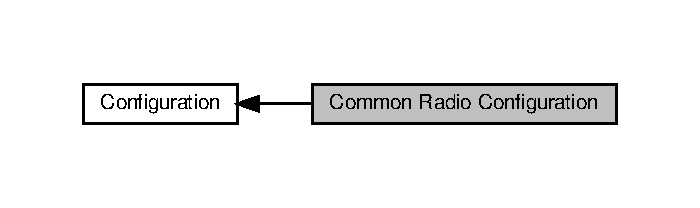
\includegraphics[width=336pt]{group__defines__radio__common__configuraiton}
\end{center}
\end{figure}
\subsection*{Macros}
\begin{DoxyCompactItemize}
\item 
\#define \hyperlink{group__defines__radio__common__configuraiton_ga3e9af6b370e370158949ba1f4d064a38}{S\+Y\+N\+C\+\_\+\+W\+O\+RD}~0x12
\item 
\#define \hyperlink{group__defines__radio__common__configuraiton_gaed963c48ead7d4a77519f1d09cffa16c}{T\+C\+X\+O\+\_\+\+V\+O\+L\+T\+A\+GE}~1.\+6
\item 
\#define \hyperlink{group__defines__radio__common__configuraiton_ga89986fbe657f799f601b5b92f7632ece}{M\+A\+X\+\_\+\+N\+U\+M\+\_\+\+O\+F\+\_\+\+B\+L\+O\+C\+KS}~3
\item 
\#define \hyperlink{group__defines__radio__common__configuraiton_ga3b4956886146ec23bf4177b7aef17b3d}{L\+O\+R\+A\+\_\+\+R\+E\+C\+E\+I\+V\+E\+\_\+\+W\+I\+N\+D\+O\+W\+\_\+\+L\+E\+N\+G\+TH}~40
\item 
\#define \hyperlink{group__defines__radio__common__configuraiton_ga6ecfb0a7dee19b5096beeafbc7289815}{F\+S\+K\+\_\+\+R\+E\+C\+E\+I\+V\+E\+\_\+\+W\+I\+N\+D\+O\+W\+\_\+\+L\+E\+N\+G\+TH}~20
\item 
\#define \hyperlink{group__defines__radio__common__configuraiton_ga897b727b895f7f0b151b7197abaeb1f6}{R\+E\+S\+P\+O\+N\+S\+E\+\_\+\+D\+E\+L\+AY}~500
\item 
\#define \hyperlink{group__defines__radio__common__configuraiton_ga9c4ea33b2371bca7b91866f44f4555b7}{W\+H\+I\+T\+E\+N\+I\+N\+G\+\_\+\+I\+N\+I\+T\+I\+AL}~0x1\+FF
\end{DoxyCompactItemize}


\subsection{Detailed Description}
\begin{DoxyRefDesc}{Test}
\item[\hyperlink{test__test000025}{Test}](ID C\+O\+N\+F\+\_\+\+R\+A\+D\+I\+O\+\_\+\+T0) (S\+EV 1) Check that the S\+Y\+N\+C\+\_\+\+W\+O\+RD is compatable with all radios and is suitable. 

(ID C\+O\+N\+F\+\_\+\+R\+A\+D\+I\+O\+\_\+\+T1) (S\+EV 1) Check that the T\+X\+C0\+\_\+\+V\+O\+L\+T\+A\+GE value is suitable. 

(ID C\+O\+N\+F\+\_\+\+R\+A\+D\+I\+O\+\_\+\+T2) (S\+EV 1) Check that the L\+O\+W\+\_\+\+P\+O\+W\+E\+R\+\_\+\+L\+E\+V\+EL is suitable. 

(ID C\+O\+N\+F\+\_\+\+R\+A\+D\+I\+O\+\_\+\+T3) (S\+EV 1) Check that the M\+A\+X\+\_\+\+N\+U\+M\+B\+E\+R\+\_\+\+O\+F\+\_\+\+B\+L\+O\+C\+KS works. 

(ID C\+O\+N\+F\+\_\+\+R\+A\+D\+I\+O\+\_\+\+T4) (S\+EV 1) Check that the L\+O\+R\+A\+\_\+\+R\+E\+C\+E\+I\+V\+E\+\_\+\+W\+I\+N\+D\+O\+W\+\_\+\+L\+E\+N\+G\+TH works. 

(ID C\+O\+N\+F\+\_\+\+R\+A\+D\+I\+O\+\_\+\+T5) (S\+EV 1) Check that the F\+S\+K\+\_\+\+R\+E\+C\+E\+I\+V\+E\+\_\+\+W\+I\+N\+D\+O\+W\+\_\+\+L\+E\+N\+G\+TH works. 

(ID C\+O\+N\+F\+\_\+\+R\+A\+D\+I\+O\+\_\+\+T6) (S\+EV 1) Check that the R\+E\+S\+P\+O\+N\+S\+E\+\_\+\+D\+E\+L\+AY is suitable and works.\end{DoxyRefDesc}


\subsection{Macro Definition Documentation}
\mbox{\Hypertarget{group__defines__radio__common__configuraiton_ga6ecfb0a7dee19b5096beeafbc7289815}\label{group__defines__radio__common__configuraiton_ga6ecfb0a7dee19b5096beeafbc7289815}} 
\index{Common Radio Configuration@{Common Radio Configuration}!F\+S\+K\+\_\+\+R\+E\+C\+E\+I\+V\+E\+\_\+\+W\+I\+N\+D\+O\+W\+\_\+\+L\+E\+N\+G\+TH@{F\+S\+K\+\_\+\+R\+E\+C\+E\+I\+V\+E\+\_\+\+W\+I\+N\+D\+O\+W\+\_\+\+L\+E\+N\+G\+TH}}
\index{F\+S\+K\+\_\+\+R\+E\+C\+E\+I\+V\+E\+\_\+\+W\+I\+N\+D\+O\+W\+\_\+\+L\+E\+N\+G\+TH@{F\+S\+K\+\_\+\+R\+E\+C\+E\+I\+V\+E\+\_\+\+W\+I\+N\+D\+O\+W\+\_\+\+L\+E\+N\+G\+TH}!Common Radio Configuration@{Common Radio Configuration}}
\subsubsection{\texorpdfstring{F\+S\+K\+\_\+\+R\+E\+C\+E\+I\+V\+E\+\_\+\+W\+I\+N\+D\+O\+W\+\_\+\+L\+E\+N\+G\+TH}{FSK\_RECEIVE\_WINDOW\_LENGTH}}
{\footnotesize\ttfamily \#define F\+S\+K\+\_\+\+R\+E\+C\+E\+I\+V\+E\+\_\+\+W\+I\+N\+D\+O\+W\+\_\+\+L\+E\+N\+G\+TH~20}

How long to listen out for F\+SK transmissions for (s) 

Definition at line 472 of file configuration.\+h.

\mbox{\Hypertarget{group__defines__radio__common__configuraiton_ga3b4956886146ec23bf4177b7aef17b3d}\label{group__defines__radio__common__configuraiton_ga3b4956886146ec23bf4177b7aef17b3d}} 
\index{Common Radio Configuration@{Common Radio Configuration}!L\+O\+R\+A\+\_\+\+R\+E\+C\+E\+I\+V\+E\+\_\+\+W\+I\+N\+D\+O\+W\+\_\+\+L\+E\+N\+G\+TH@{L\+O\+R\+A\+\_\+\+R\+E\+C\+E\+I\+V\+E\+\_\+\+W\+I\+N\+D\+O\+W\+\_\+\+L\+E\+N\+G\+TH}}
\index{L\+O\+R\+A\+\_\+\+R\+E\+C\+E\+I\+V\+E\+\_\+\+W\+I\+N\+D\+O\+W\+\_\+\+L\+E\+N\+G\+TH@{L\+O\+R\+A\+\_\+\+R\+E\+C\+E\+I\+V\+E\+\_\+\+W\+I\+N\+D\+O\+W\+\_\+\+L\+E\+N\+G\+TH}!Common Radio Configuration@{Common Radio Configuration}}
\subsubsection{\texorpdfstring{L\+O\+R\+A\+\_\+\+R\+E\+C\+E\+I\+V\+E\+\_\+\+W\+I\+N\+D\+O\+W\+\_\+\+L\+E\+N\+G\+TH}{LORA\_RECEIVE\_WINDOW\_LENGTH}}
{\footnotesize\ttfamily \#define L\+O\+R\+A\+\_\+\+R\+E\+C\+E\+I\+V\+E\+\_\+\+W\+I\+N\+D\+O\+W\+\_\+\+L\+E\+N\+G\+TH~40}

How long to listen out for Lo\+Ra transmissions for (s) 

Definition at line 471 of file configuration.\+h.

\mbox{\Hypertarget{group__defines__radio__common__configuraiton_ga89986fbe657f799f601b5b92f7632ece}\label{group__defines__radio__common__configuraiton_ga89986fbe657f799f601b5b92f7632ece}} 
\index{Common Radio Configuration@{Common Radio Configuration}!M\+A\+X\+\_\+\+N\+U\+M\+\_\+\+O\+F\+\_\+\+B\+L\+O\+C\+KS@{M\+A\+X\+\_\+\+N\+U\+M\+\_\+\+O\+F\+\_\+\+B\+L\+O\+C\+KS}}
\index{M\+A\+X\+\_\+\+N\+U\+M\+\_\+\+O\+F\+\_\+\+B\+L\+O\+C\+KS@{M\+A\+X\+\_\+\+N\+U\+M\+\_\+\+O\+F\+\_\+\+B\+L\+O\+C\+KS}!Common Radio Configuration@{Common Radio Configuration}}
\subsubsection{\texorpdfstring{M\+A\+X\+\_\+\+N\+U\+M\+\_\+\+O\+F\+\_\+\+B\+L\+O\+C\+KS}{MAX\_NUM\_OF\_BLOCKS}}
{\footnotesize\ttfamily \#define M\+A\+X\+\_\+\+N\+U\+M\+\_\+\+O\+F\+\_\+\+B\+L\+O\+C\+KS~3}

maximum number of A\+E\+S128 blocks that will be accepted 

Definition at line 470 of file configuration.\+h.

\mbox{\Hypertarget{group__defines__radio__common__configuraiton_ga897b727b895f7f0b151b7197abaeb1f6}\label{group__defines__radio__common__configuraiton_ga897b727b895f7f0b151b7197abaeb1f6}} 
\index{Common Radio Configuration@{Common Radio Configuration}!R\+E\+S\+P\+O\+N\+S\+E\+\_\+\+D\+E\+L\+AY@{R\+E\+S\+P\+O\+N\+S\+E\+\_\+\+D\+E\+L\+AY}}
\index{R\+E\+S\+P\+O\+N\+S\+E\+\_\+\+D\+E\+L\+AY@{R\+E\+S\+P\+O\+N\+S\+E\+\_\+\+D\+E\+L\+AY}!Common Radio Configuration@{Common Radio Configuration}}
\subsubsection{\texorpdfstring{R\+E\+S\+P\+O\+N\+S\+E\+\_\+\+D\+E\+L\+AY}{RESPONSE\_DELAY}}
{\footnotesize\ttfamily \#define R\+E\+S\+P\+O\+N\+S\+E\+\_\+\+D\+E\+L\+AY~500}

How long to wait for before responding/processing a transmission (ms) 

Definition at line 473 of file configuration.\+h.

\mbox{\Hypertarget{group__defines__radio__common__configuraiton_ga3e9af6b370e370158949ba1f4d064a38}\label{group__defines__radio__common__configuraiton_ga3e9af6b370e370158949ba1f4d064a38}} 
\index{Common Radio Configuration@{Common Radio Configuration}!S\+Y\+N\+C\+\_\+\+W\+O\+RD@{S\+Y\+N\+C\+\_\+\+W\+O\+RD}}
\index{S\+Y\+N\+C\+\_\+\+W\+O\+RD@{S\+Y\+N\+C\+\_\+\+W\+O\+RD}!Common Radio Configuration@{Common Radio Configuration}}
\subsubsection{\texorpdfstring{S\+Y\+N\+C\+\_\+\+W\+O\+RD}{SYNC\_WORD}}
{\footnotesize\ttfamily \#define S\+Y\+N\+C\+\_\+\+W\+O\+RD~0x12}

Ensure this sync word is compatable with all devices. 

Definition at line 468 of file configuration.\+h.

\mbox{\Hypertarget{group__defines__radio__common__configuraiton_gaed963c48ead7d4a77519f1d09cffa16c}\label{group__defines__radio__common__configuraiton_gaed963c48ead7d4a77519f1d09cffa16c}} 
\index{Common Radio Configuration@{Common Radio Configuration}!T\+C\+X\+O\+\_\+\+V\+O\+L\+T\+A\+GE@{T\+C\+X\+O\+\_\+\+V\+O\+L\+T\+A\+GE}}
\index{T\+C\+X\+O\+\_\+\+V\+O\+L\+T\+A\+GE@{T\+C\+X\+O\+\_\+\+V\+O\+L\+T\+A\+GE}!Common Radio Configuration@{Common Radio Configuration}}
\subsubsection{\texorpdfstring{T\+C\+X\+O\+\_\+\+V\+O\+L\+T\+A\+GE}{TCXO\_VOLTAGE}}
{\footnotesize\ttfamily \#define T\+C\+X\+O\+\_\+\+V\+O\+L\+T\+A\+GE~1.\+6}

Sets the radio\textquotesingle{}s T\+C\+X0 voltage. (V) 

Definition at line 469 of file configuration.\+h.

\mbox{\Hypertarget{group__defines__radio__common__configuraiton_ga9c4ea33b2371bca7b91866f44f4555b7}\label{group__defines__radio__common__configuraiton_ga9c4ea33b2371bca7b91866f44f4555b7}} 
\index{Common Radio Configuration@{Common Radio Configuration}!W\+H\+I\+T\+E\+N\+I\+N\+G\+\_\+\+I\+N\+I\+T\+I\+AL@{W\+H\+I\+T\+E\+N\+I\+N\+G\+\_\+\+I\+N\+I\+T\+I\+AL}}
\index{W\+H\+I\+T\+E\+N\+I\+N\+G\+\_\+\+I\+N\+I\+T\+I\+AL@{W\+H\+I\+T\+E\+N\+I\+N\+G\+\_\+\+I\+N\+I\+T\+I\+AL}!Common Radio Configuration@{Common Radio Configuration}}
\subsubsection{\texorpdfstring{W\+H\+I\+T\+E\+N\+I\+N\+G\+\_\+\+I\+N\+I\+T\+I\+AL}{WHITENING\_INITIAL}}
{\footnotesize\ttfamily \#define W\+H\+I\+T\+E\+N\+I\+N\+G\+\_\+\+I\+N\+I\+T\+I\+AL~0x1\+FF}

Whitening L\+F\+SR initial value, to ensure S\+X127x compatibility 

Definition at line 474 of file configuration.\+h.


\hypertarget{group__defines__radio__lora__configuration}{}\section{Lo\+Ra Radio Configuration}
\label{group__defines__radio__lora__configuration}\index{Lo\+Ra Radio Configuration@{Lo\+Ra Radio Configuration}}


\tabulinesep=1mm
\begin{longtabu} spread 0pt [c]{*{3}{|X[-1]}|}
\hline
\rowcolor{\tableheadbgcolor}\textbf{ Description}&\textbf{ Value}&\textbf{ Units  }\\\cline{1-3}
\endfirsthead
\hline
\endfoot
\hline
\rowcolor{\tableheadbgcolor}\textbf{ Description}&\textbf{ Value}&\textbf{ Units  }\\\cline{1-3}
\endhead
Carrier Frequency.&436.\+7&M\+Hz \\\cline{1-3}
Bandwidth.&125.\+0&K\+Hz dual sideband \\\cline{1-3}
Spreading Factor.&11&N/A \\\cline{1-3}
Spreading Factor Alternate.&10&N/A \\\cline{1-3}
Coding rate.&8 (4/8 Extended Hamming)&N/A \\\cline{1-3}
Output Power.&20&d\+Bm \\\cline{1-3}
Current limit.&160.\+0&mA \\\cline{1-3}
\end{longtabu}
 


Collaboration diagram for Lo\+Ra Radio Configuration\+:
\nopagebreak
\begin{figure}[H]
\begin{center}
\leavevmode
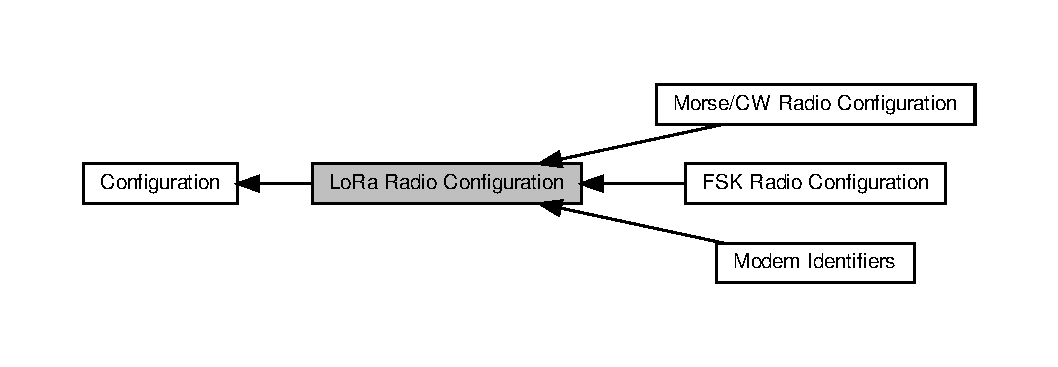
\includegraphics[width=350pt]{group__defines__radio__lora__configuration}
\end{center}
\end{figure}
\subsection*{Modules}
\begin{DoxyCompactItemize}
\item 
\hyperlink{group__defines__radio__non__ism__band__fsk__configuraiton}{F\+S\+K Radio Configuration}
\begin{DoxyCompactList}\small\item\em \tabulinesep=1mm
\begin{longtabu} spread 0pt [c]{*{3}{|X[-1]}|}
\hline
\rowcolor{\tableheadbgcolor}\textbf{ Description}&\textbf{ Value}&\textbf{ Units  }\\\cline{1-3}
\endfirsthead
\hline
\endfoot
\hline
\rowcolor{\tableheadbgcolor}\textbf{ Description}&\textbf{ Value}&\textbf{ Units  }\\\cline{1-3}
\endhead
Carrier Frequency.&436.\+7&M\+Hz \\\cline{1-3}
Bit Rate.&9.\+6&Kbps \\\cline{1-3}
Frequency Deviation.&5.\+0&K\+Hz single-\/sideband \\\cline{1-3}
RX Bandwidth.&19.\+5&K\+Hz single-\/sideband \\\cline{1-3}
Output Power.&20&d\+Bm \\\cline{1-3}
Preamble Length.&16&bits \\\cline{1-3}
Data Shaping.&0.\+5&G\+F\+SK filter BT product \\\cline{1-3}
Current Limit.&160.\+0&mA \\\cline{1-3}
\end{longtabu}
\end{DoxyCompactList}\item 
\hyperlink{group__defines__radio__morse__cw__configuration}{Morse/\+C\+W Radio Configuration}
\item 
\hyperlink{group__defines__radio__modem__configuration}{Modem Identifiers}
\end{DoxyCompactItemize}
\subsection*{Macros}
\begin{DoxyCompactItemize}
\item 
\#define \hyperlink{group__defines__radio__lora__configuration_gafe832936c374bff5e188c400514308a8}{L\+O\+R\+A\+\_\+\+C\+A\+R\+R\+I\+E\+R\+\_\+\+F\+R\+E\+Q\+U\+E\+N\+CY}~436.\+7
\item 
\#define \hyperlink{group__defines__radio__lora__configuration_ga33702007527b9cea6e029b919322a7a5}{L\+O\+R\+A\+\_\+\+B\+A\+N\+D\+W\+I\+D\+TH}~125.\+0
\item 
\mbox{\Hypertarget{group__defines__radio__lora__configuration_ga58e25fd82f3b77562dde8259fef5e79a}\label{group__defines__radio__lora__configuration_ga58e25fd82f3b77562dde8259fef5e79a}} 
\#define {\bfseries L\+O\+R\+A\+\_\+\+S\+P\+R\+E\+A\+D\+I\+N\+G\+\_\+\+F\+A\+C\+T\+OR}~11
\item 
\mbox{\Hypertarget{group__defines__radio__lora__configuration_ga0c17009e87781d98337738f175ee3238}\label{group__defines__radio__lora__configuration_ga0c17009e87781d98337738f175ee3238}} 
\#define {\bfseries L\+O\+R\+A\+\_\+\+S\+P\+R\+E\+A\+D\+I\+N\+G\+\_\+\+F\+A\+C\+T\+O\+R\+\_\+\+A\+LT}~10
\item 
\#define \hyperlink{group__defines__radio__lora__configuration_ga4c6536f4c2d7ce68b90100bf64d7c17e}{L\+O\+R\+A\+\_\+\+C\+O\+D\+I\+N\+G\+\_\+\+R\+A\+TE}~8
\item 
\#define \hyperlink{group__defines__radio__lora__configuration_ga85f023404afa6ec72b6dc7fbfe6742f5}{L\+O\+R\+A\+\_\+\+O\+U\+T\+P\+U\+T\+\_\+\+P\+O\+W\+ER}~20
\item 
\#define \hyperlink{group__defines__radio__lora__configuration_ga65acce91212130f161b96ae5003a503c}{L\+O\+R\+A\+\_\+\+C\+U\+R\+R\+E\+N\+T\+\_\+\+L\+I\+M\+IT}~140.\+0
\end{DoxyCompactItemize}


\subsection{Detailed Description}
\tabulinesep=1mm
\begin{longtabu} spread 0pt [c]{*{3}{|X[-1]}|}
\hline
\rowcolor{\tableheadbgcolor}\textbf{ Description}&\textbf{ Value}&\textbf{ Units  }\\\cline{1-3}
\endfirsthead
\hline
\endfoot
\hline
\rowcolor{\tableheadbgcolor}\textbf{ Description}&\textbf{ Value}&\textbf{ Units  }\\\cline{1-3}
\endhead
Carrier Frequency.&436.\+7&M\+Hz \\\cline{1-3}
Bandwidth.&125.\+0&K\+Hz dual sideband \\\cline{1-3}
Spreading Factor.&11&N/A \\\cline{1-3}
Spreading Factor Alternate.&10&N/A \\\cline{1-3}
Coding rate.&8 (4/8 Extended Hamming)&N/A \\\cline{1-3}
Output Power.&20&d\+Bm \\\cline{1-3}
Current limit.&160.\+0&mA \\\cline{1-3}
\end{longtabu}


\begin{DoxyRefDesc}{Todo}
\item[\hyperlink{todo__todo000004}{Todo}]Julian -\/$>$ double check these values please. \end{DoxyRefDesc}
\begin{DoxyRefDesc}{Test}
\item[\hyperlink{test__test000026}{Test}]Test that we can receive Lo\+Ra transmissions from the satellite with these default parameters 

(ID C\+O\+N\+F\+\_\+\+L\+O\+R\+A\+\_\+\+R\+A\+D\+I\+O\+\_\+\+T1) (S\+EV 1) Check that the radio transmits at L\+O\+R\+A\+\_\+\+B\+A\+N\+D\+W\+I\+D\+TH. 

(ID C\+O\+N\+F\+\_\+\+L\+O\+R\+A\+\_\+\+R\+A\+D\+I\+O\+\_\+\+T2) (S\+EV 1) Check that the radio is transmitting at L\+O\+R\+A\+\_\+\+S\+P\+R\+E\+A\+D\+I\+N\+G\+\_\+\+F\+A\+C\+T\+OR. 

(ID C\+O\+N\+F\+\_\+\+L\+O\+R\+A\+\_\+\+R\+A\+D\+I\+O\+\_\+\+T3) (S\+EV 1) Check that the radio can/is transmitting at L\+O\+R\+A\+\_\+\+S\+P\+R\+E\+A\+D\+I\+N\+G\+\_\+\+F\+A\+C\+T\+O\+R\+\_\+\+A\+LT. 

(ID C\+O\+N\+F\+\_\+\+L\+O\+R\+A\+\_\+\+R\+A\+D\+I\+O\+\_\+\+T4) (S\+EV 1) Check that the radio is transmitting at L\+O\+R\+A\+\_\+\+C\+O\+D\+I\+N\+G\+\_\+\+R\+A\+TE. 

(ID C\+O\+N\+F\+\_\+\+L\+O\+R\+A\+\_\+\+R\+A\+D\+I\+O\+\_\+\+T5) (S\+EV 1) Check that the radio is transmitting at L\+O\+R\+A\+\_\+\+O\+U\+T\+P\+U\+T\+\_\+\+P\+O\+W\+ER. 

(ID C\+O\+N\+F\+\_\+\+L\+O\+R\+A\+\_\+\+R\+A\+D\+I\+O\+\_\+\+T6) (S\+EV 1) Check that the radio draws no more than 160.\+0mA.\end{DoxyRefDesc}


\begin{DoxyRefDesc}{Test}
\item[\hyperlink{test__test000027}{Test}](ID C\+O\+N\+F\+\_\+\+L\+O\+R\+A\+\_\+\+R\+A\+D\+I\+O\+\_\+\+T0) (S\+EV 1) Check that the radio transmits lora at L\+O\+R\+A\+\_\+\+C\+A\+R\+R\+I\+E\+R\+\_\+\+F\+R\+E\+Q\+U\+E\+N\+CY. \end{DoxyRefDesc}


\subsection{Macro Definition Documentation}
\mbox{\Hypertarget{group__defines__radio__lora__configuration_ga33702007527b9cea6e029b919322a7a5}\label{group__defines__radio__lora__configuration_ga33702007527b9cea6e029b919322a7a5}} 
\index{Lo\+Ra Radio Configuration@{Lo\+Ra Radio Configuration}!L\+O\+R\+A\+\_\+\+B\+A\+N\+D\+W\+I\+D\+TH@{L\+O\+R\+A\+\_\+\+B\+A\+N\+D\+W\+I\+D\+TH}}
\index{L\+O\+R\+A\+\_\+\+B\+A\+N\+D\+W\+I\+D\+TH@{L\+O\+R\+A\+\_\+\+B\+A\+N\+D\+W\+I\+D\+TH}!Lo\+Ra Radio Configuration@{Lo\+Ra Radio Configuration}}
\subsubsection{\texorpdfstring{L\+O\+R\+A\+\_\+\+B\+A\+N\+D\+W\+I\+D\+TH}{LORA\_BANDWIDTH}}
{\footnotesize\ttfamily \#define L\+O\+R\+A\+\_\+\+B\+A\+N\+D\+W\+I\+D\+TH~125.\+0}

k\+Hz dual sideband 

Definition at line 507 of file configuration.\+h.

\mbox{\Hypertarget{group__defines__radio__lora__configuration_gafe832936c374bff5e188c400514308a8}\label{group__defines__radio__lora__configuration_gafe832936c374bff5e188c400514308a8}} 
\index{Lo\+Ra Radio Configuration@{Lo\+Ra Radio Configuration}!L\+O\+R\+A\+\_\+\+C\+A\+R\+R\+I\+E\+R\+\_\+\+F\+R\+E\+Q\+U\+E\+N\+CY@{L\+O\+R\+A\+\_\+\+C\+A\+R\+R\+I\+E\+R\+\_\+\+F\+R\+E\+Q\+U\+E\+N\+CY}}
\index{L\+O\+R\+A\+\_\+\+C\+A\+R\+R\+I\+E\+R\+\_\+\+F\+R\+E\+Q\+U\+E\+N\+CY@{L\+O\+R\+A\+\_\+\+C\+A\+R\+R\+I\+E\+R\+\_\+\+F\+R\+E\+Q\+U\+E\+N\+CY}!Lo\+Ra Radio Configuration@{Lo\+Ra Radio Configuration}}
\subsubsection{\texorpdfstring{L\+O\+R\+A\+\_\+\+C\+A\+R\+R\+I\+E\+R\+\_\+\+F\+R\+E\+Q\+U\+E\+N\+CY}{LORA\_CARRIER\_FREQUENCY}}
{\footnotesize\ttfamily \#define L\+O\+R\+A\+\_\+\+C\+A\+R\+R\+I\+E\+R\+\_\+\+F\+R\+E\+Q\+U\+E\+N\+CY~436.\+7}

M\+Hz 

Definition at line 506 of file configuration.\+h.

\mbox{\Hypertarget{group__defines__radio__lora__configuration_ga4c6536f4c2d7ce68b90100bf64d7c17e}\label{group__defines__radio__lora__configuration_ga4c6536f4c2d7ce68b90100bf64d7c17e}} 
\index{Lo\+Ra Radio Configuration@{Lo\+Ra Radio Configuration}!L\+O\+R\+A\+\_\+\+C\+O\+D\+I\+N\+G\+\_\+\+R\+A\+TE@{L\+O\+R\+A\+\_\+\+C\+O\+D\+I\+N\+G\+\_\+\+R\+A\+TE}}
\index{L\+O\+R\+A\+\_\+\+C\+O\+D\+I\+N\+G\+\_\+\+R\+A\+TE@{L\+O\+R\+A\+\_\+\+C\+O\+D\+I\+N\+G\+\_\+\+R\+A\+TE}!Lo\+Ra Radio Configuration@{Lo\+Ra Radio Configuration}}
\subsubsection{\texorpdfstring{L\+O\+R\+A\+\_\+\+C\+O\+D\+I\+N\+G\+\_\+\+R\+A\+TE}{LORA\_CODING\_RATE}}
{\footnotesize\ttfamily \#define L\+O\+R\+A\+\_\+\+C\+O\+D\+I\+N\+G\+\_\+\+R\+A\+TE~8}

4/8, Extended Hamming 

Definition at line 510 of file configuration.\+h.

\mbox{\Hypertarget{group__defines__radio__lora__configuration_ga65acce91212130f161b96ae5003a503c}\label{group__defines__radio__lora__configuration_ga65acce91212130f161b96ae5003a503c}} 
\index{Lo\+Ra Radio Configuration@{Lo\+Ra Radio Configuration}!L\+O\+R\+A\+\_\+\+C\+U\+R\+R\+E\+N\+T\+\_\+\+L\+I\+M\+IT@{L\+O\+R\+A\+\_\+\+C\+U\+R\+R\+E\+N\+T\+\_\+\+L\+I\+M\+IT}}
\index{L\+O\+R\+A\+\_\+\+C\+U\+R\+R\+E\+N\+T\+\_\+\+L\+I\+M\+IT@{L\+O\+R\+A\+\_\+\+C\+U\+R\+R\+E\+N\+T\+\_\+\+L\+I\+M\+IT}!Lo\+Ra Radio Configuration@{Lo\+Ra Radio Configuration}}
\subsubsection{\texorpdfstring{L\+O\+R\+A\+\_\+\+C\+U\+R\+R\+E\+N\+T\+\_\+\+L\+I\+M\+IT}{LORA\_CURRENT\_LIMIT}}
{\footnotesize\ttfamily \#define L\+O\+R\+A\+\_\+\+C\+U\+R\+R\+E\+N\+T\+\_\+\+L\+I\+M\+IT~140.\+0}

mA 

Definition at line 512 of file configuration.\+h.

\mbox{\Hypertarget{group__defines__radio__lora__configuration_ga85f023404afa6ec72b6dc7fbfe6742f5}\label{group__defines__radio__lora__configuration_ga85f023404afa6ec72b6dc7fbfe6742f5}} 
\index{Lo\+Ra Radio Configuration@{Lo\+Ra Radio Configuration}!L\+O\+R\+A\+\_\+\+O\+U\+T\+P\+U\+T\+\_\+\+P\+O\+W\+ER@{L\+O\+R\+A\+\_\+\+O\+U\+T\+P\+U\+T\+\_\+\+P\+O\+W\+ER}}
\index{L\+O\+R\+A\+\_\+\+O\+U\+T\+P\+U\+T\+\_\+\+P\+O\+W\+ER@{L\+O\+R\+A\+\_\+\+O\+U\+T\+P\+U\+T\+\_\+\+P\+O\+W\+ER}!Lo\+Ra Radio Configuration@{Lo\+Ra Radio Configuration}}
\subsubsection{\texorpdfstring{L\+O\+R\+A\+\_\+\+O\+U\+T\+P\+U\+T\+\_\+\+P\+O\+W\+ER}{LORA\_OUTPUT\_POWER}}
{\footnotesize\ttfamily \#define L\+O\+R\+A\+\_\+\+O\+U\+T\+P\+U\+T\+\_\+\+P\+O\+W\+ER~20}

d\+Bm 

Definition at line 511 of file configuration.\+h.


\hypertarget{group__defines__radio__non__ism__band__fsk__configuraiton}{}\section{F\+SK Radio Configuration}
\label{group__defines__radio__non__ism__band__fsk__configuraiton}\index{F\+S\+K Radio Configuration@{F\+S\+K Radio Configuration}}


\tabulinesep=1mm
\begin{longtabu} spread 0pt [c]{*{3}{|X[-1]}|}
\hline
\rowcolor{\tableheadbgcolor}\textbf{ Description}&\textbf{ Value}&\textbf{ Units  }\\\cline{1-3}
\endfirsthead
\hline
\endfoot
\hline
\rowcolor{\tableheadbgcolor}\textbf{ Description}&\textbf{ Value}&\textbf{ Units  }\\\cline{1-3}
\endhead
Carrier Frequency.&436.\+7&M\+Hz \\\cline{1-3}
Bit Rate.&9.\+6&Kbps \\\cline{1-3}
Frequency Deviation.&5.\+0&K\+Hz single-\/sideband \\\cline{1-3}
RX Bandwidth.&19.\+5&K\+Hz single-\/sideband \\\cline{1-3}
Output Power.&20&d\+Bm \\\cline{1-3}
Preamble Length.&16&bits \\\cline{1-3}
Data Shaping.&0.\+5&G\+F\+SK filter BT product \\\cline{1-3}
Current Limit.&160.\+0&mA \\\cline{1-3}
\end{longtabu}
 


Collaboration diagram for F\+SK Radio Configuration\+:
\nopagebreak
\begin{figure}[H]
\begin{center}
\leavevmode
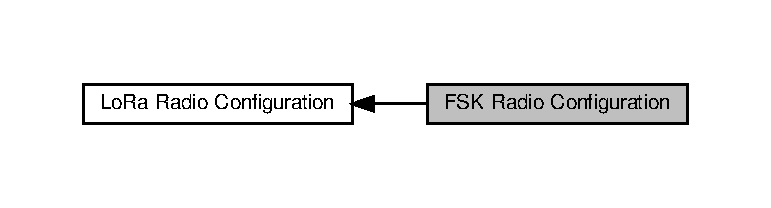
\includegraphics[width=350pt]{group__defines__radio__non__ism__band__fsk__configuraiton}
\end{center}
\end{figure}
\subsection*{Macros}
\begin{DoxyCompactItemize}
\item 
\#define \hyperlink{group__defines__radio__non__ism__band__fsk__configuraiton_ga0c165cacd352a37567effed3f405492e}{F\+S\+K\+\_\+\+C\+A\+R\+R\+I\+E\+R\+\_\+\+F\+R\+E\+Q\+U\+E\+N\+CY}~436.\+8
\item 
\#define \hyperlink{group__defines__radio__non__ism__band__fsk__configuraiton_ga0e39a8b8bddb39a81db0e1296f547f2d}{F\+S\+K\+\_\+\+B\+I\+T\+\_\+\+R\+A\+TE}~9.\+6
\item 
\#define \hyperlink{group__defines__radio__non__ism__band__fsk__configuraiton_ga9bd34bff3c7ef520993a7d85973701ab}{F\+S\+K\+\_\+\+F\+R\+E\+Q\+U\+E\+N\+C\+Y\+\_\+\+D\+E\+V\+I\+A\+T\+I\+ON}~5.\+0
\item 
\#define \hyperlink{group__defines__radio__non__ism__band__fsk__configuraiton_ga4776d889dbe10a9451f6f599301da027}{F\+S\+K\+\_\+\+R\+X\+\_\+\+B\+A\+N\+D\+W\+I\+D\+TH}~39.\+0
\item 
\#define \hyperlink{group__defines__radio__non__ism__band__fsk__configuraiton_ga43a05b43583e7ca3f06ec418e80e0806}{F\+S\+K\+\_\+\+O\+U\+T\+P\+U\+T\+\_\+\+P\+O\+W\+ER}~20
\item 
\#define \hyperlink{group__defines__radio__non__ism__band__fsk__configuraiton_ga8e2bfafd0ea1783188ce2accaa282559}{F\+S\+K\+\_\+\+P\+R\+E\+A\+M\+B\+L\+E\+\_\+\+L\+E\+N\+G\+TH}~16
\item 
\#define \hyperlink{group__defines__radio__non__ism__band__fsk__configuraiton_ga0a39133f38cb54fb6fa6460518e84b38}{F\+S\+K\+\_\+\+D\+A\+T\+A\+\_\+\+S\+H\+A\+P\+I\+NG}~0.\+5
\item 
\#define \hyperlink{group__defines__radio__non__ism__band__fsk__configuraiton_gac8f3dda4754cbba6b8912fc5653e597d}{F\+S\+K\+\_\+\+C\+U\+R\+R\+E\+N\+T\+\_\+\+L\+I\+M\+IT}~140.\+0
\end{DoxyCompactItemize}


\subsection{Detailed Description}
\tabulinesep=1mm
\begin{longtabu} spread 0pt [c]{*{3}{|X[-1]}|}
\hline
\rowcolor{\tableheadbgcolor}\textbf{ Description}&\textbf{ Value}&\textbf{ Units  }\\\cline{1-3}
\endfirsthead
\hline
\endfoot
\hline
\rowcolor{\tableheadbgcolor}\textbf{ Description}&\textbf{ Value}&\textbf{ Units  }\\\cline{1-3}
\endhead
Carrier Frequency.&436.\+7&M\+Hz \\\cline{1-3}
Bit Rate.&9.\+6&Kbps \\\cline{1-3}
Frequency Deviation.&5.\+0&K\+Hz single-\/sideband \\\cline{1-3}
RX Bandwidth.&19.\+5&K\+Hz single-\/sideband \\\cline{1-3}
Output Power.&20&d\+Bm \\\cline{1-3}
Preamble Length.&16&bits \\\cline{1-3}
Data Shaping.&0.\+5&G\+F\+SK filter BT product \\\cline{1-3}
Current Limit.&160.\+0&mA \\\cline{1-3}
\end{longtabu}


\begin{DoxyRefDesc}{Todo}
\item[\hyperlink{todo__todo000005}{Todo}]check F\+S\+K\+\_\+\+R\+X\+\_\+\+B\+A\+N\+D\+W\+I\+D\+TH value\end{DoxyRefDesc}


\begin{DoxyRefDesc}{Test}
\item[\hyperlink{test__test000028}{Test}](ID C\+O\+N\+F\+\_\+\+F\+S\+K\+\_\+\+R\+A\+D\+I\+O\+\_\+\+T0) (S\+EV 1) Check that the radio functions at F\+S\+K\+\_\+\+C\+A\+R\+R\+I\+E\+R\+\_\+\+F\+R\+E\+Q\+U\+E\+N\+CY. 

(ID C\+O\+N\+F\+\_\+\+F\+S\+K\+\_\+\+R\+A\+D\+I\+O\+\_\+\+T1) (S\+EV 1) Check that the radio functions with bit rate of F\+S\+K\+\_\+\+B\+I\+T\+\_\+\+R\+A\+TE. 

(ID C\+O\+N\+F\+\_\+\+F\+S\+K\+\_\+\+R\+A\+D\+I\+O\+\_\+\+T2) (S\+EV 1) Check that the radio functions with a frequency deviation of F\+S\+K\+\_\+\+F\+R\+E\+Q\+U\+E\+N\+C\+Y\+\_\+\+D\+E\+V\+I\+A\+T\+I\+ON. 

(ID C\+O\+N\+F\+\_\+\+F\+S\+K\+\_\+\+R\+A\+D\+I\+O\+\_\+\+T3) (S\+EV 1) Check that the radio receives F\+SK messages at F\+S\+K\+\_\+\+R\+X\+\_\+\+B\+A\+N\+D\+W\+I\+D\+TH. 

(ID C\+O\+N\+F\+\_\+\+F\+S\+K\+\_\+\+R\+A\+D\+I\+O\+\_\+\+T4) (S\+EV 1) Check that the radio outputs at F\+S\+K\+\_\+\+O\+U\+T\+P\+U\+T\+\_\+\+P\+O\+W\+ER. 

(ID C\+O\+N\+F\+\_\+\+F\+S\+K\+\_\+\+R\+A\+D\+I\+O\+\_\+\+T5) (S\+EV 1) Check that the radio preamble is F\+S\+K\+\_\+\+P\+R\+E\+A\+M\+B\+L\+E\+\_\+\+L\+E\+N\+G\+TH. 

(ID C\+O\+N\+F\+\_\+\+F\+S\+K\+\_\+\+R\+A\+D\+I\+O\+\_\+\+T6) (S\+EV 1) Check that the data shaping is F\+S\+K\+\_\+\+D\+A\+T\+A\+\_\+\+S\+H\+A\+P\+I\+NG. 

(ID C\+O\+N\+F\+\_\+\+F\+S\+K\+\_\+\+R\+A\+D\+I\+O\+\_\+\+T7) (S\+EV 1) Check that the maximum drawn current is no more than F\+S\+K\+\_\+\+C\+U\+R\+R\+E\+N\+T\+\_\+\+L\+I\+M\+IT.\end{DoxyRefDesc}


\subsection{Macro Definition Documentation}
\mbox{\Hypertarget{group__defines__radio__non__ism__band__fsk__configuraiton_ga0e39a8b8bddb39a81db0e1296f547f2d}\label{group__defines__radio__non__ism__band__fsk__configuraiton_ga0e39a8b8bddb39a81db0e1296f547f2d}} 
\index{F\+S\+K Radio Configuration@{F\+S\+K Radio Configuration}!F\+S\+K\+\_\+\+B\+I\+T\+\_\+\+R\+A\+TE@{F\+S\+K\+\_\+\+B\+I\+T\+\_\+\+R\+A\+TE}}
\index{F\+S\+K\+\_\+\+B\+I\+T\+\_\+\+R\+A\+TE@{F\+S\+K\+\_\+\+B\+I\+T\+\_\+\+R\+A\+TE}!F\+S\+K Radio Configuration@{F\+S\+K Radio Configuration}}
\subsubsection{\texorpdfstring{F\+S\+K\+\_\+\+B\+I\+T\+\_\+\+R\+A\+TE}{FSK\_BIT\_RATE}}
{\footnotesize\ttfamily \#define F\+S\+K\+\_\+\+B\+I\+T\+\_\+\+R\+A\+TE~9.\+6}

kbps nominal 

Definition at line 543 of file configuration.\+h.

\mbox{\Hypertarget{group__defines__radio__non__ism__band__fsk__configuraiton_ga0c165cacd352a37567effed3f405492e}\label{group__defines__radio__non__ism__band__fsk__configuraiton_ga0c165cacd352a37567effed3f405492e}} 
\index{F\+S\+K Radio Configuration@{F\+S\+K Radio Configuration}!F\+S\+K\+\_\+\+C\+A\+R\+R\+I\+E\+R\+\_\+\+F\+R\+E\+Q\+U\+E\+N\+CY@{F\+S\+K\+\_\+\+C\+A\+R\+R\+I\+E\+R\+\_\+\+F\+R\+E\+Q\+U\+E\+N\+CY}}
\index{F\+S\+K\+\_\+\+C\+A\+R\+R\+I\+E\+R\+\_\+\+F\+R\+E\+Q\+U\+E\+N\+CY@{F\+S\+K\+\_\+\+C\+A\+R\+R\+I\+E\+R\+\_\+\+F\+R\+E\+Q\+U\+E\+N\+CY}!F\+S\+K Radio Configuration@{F\+S\+K Radio Configuration}}
\subsubsection{\texorpdfstring{F\+S\+K\+\_\+\+C\+A\+R\+R\+I\+E\+R\+\_\+\+F\+R\+E\+Q\+U\+E\+N\+CY}{FSK\_CARRIER\_FREQUENCY}}
{\footnotesize\ttfamily \#define F\+S\+K\+\_\+\+C\+A\+R\+R\+I\+E\+R\+\_\+\+F\+R\+E\+Q\+U\+E\+N\+CY~436.\+8}

M\+Hz 

Definition at line 542 of file configuration.\+h.

\mbox{\Hypertarget{group__defines__radio__non__ism__band__fsk__configuraiton_gac8f3dda4754cbba6b8912fc5653e597d}\label{group__defines__radio__non__ism__band__fsk__configuraiton_gac8f3dda4754cbba6b8912fc5653e597d}} 
\index{F\+S\+K Radio Configuration@{F\+S\+K Radio Configuration}!F\+S\+K\+\_\+\+C\+U\+R\+R\+E\+N\+T\+\_\+\+L\+I\+M\+IT@{F\+S\+K\+\_\+\+C\+U\+R\+R\+E\+N\+T\+\_\+\+L\+I\+M\+IT}}
\index{F\+S\+K\+\_\+\+C\+U\+R\+R\+E\+N\+T\+\_\+\+L\+I\+M\+IT@{F\+S\+K\+\_\+\+C\+U\+R\+R\+E\+N\+T\+\_\+\+L\+I\+M\+IT}!F\+S\+K Radio Configuration@{F\+S\+K Radio Configuration}}
\subsubsection{\texorpdfstring{F\+S\+K\+\_\+\+C\+U\+R\+R\+E\+N\+T\+\_\+\+L\+I\+M\+IT}{FSK\_CURRENT\_LIMIT}}
{\footnotesize\ttfamily \#define F\+S\+K\+\_\+\+C\+U\+R\+R\+E\+N\+T\+\_\+\+L\+I\+M\+IT~140.\+0}

mA 

Definition at line 549 of file configuration.\+h.

\mbox{\Hypertarget{group__defines__radio__non__ism__band__fsk__configuraiton_ga0a39133f38cb54fb6fa6460518e84b38}\label{group__defines__radio__non__ism__band__fsk__configuraiton_ga0a39133f38cb54fb6fa6460518e84b38}} 
\index{F\+S\+K Radio Configuration@{F\+S\+K Radio Configuration}!F\+S\+K\+\_\+\+D\+A\+T\+A\+\_\+\+S\+H\+A\+P\+I\+NG@{F\+S\+K\+\_\+\+D\+A\+T\+A\+\_\+\+S\+H\+A\+P\+I\+NG}}
\index{F\+S\+K\+\_\+\+D\+A\+T\+A\+\_\+\+S\+H\+A\+P\+I\+NG@{F\+S\+K\+\_\+\+D\+A\+T\+A\+\_\+\+S\+H\+A\+P\+I\+NG}!F\+S\+K Radio Configuration@{F\+S\+K Radio Configuration}}
\subsubsection{\texorpdfstring{F\+S\+K\+\_\+\+D\+A\+T\+A\+\_\+\+S\+H\+A\+P\+I\+NG}{FSK\_DATA\_SHAPING}}
{\footnotesize\ttfamily \#define F\+S\+K\+\_\+\+D\+A\+T\+A\+\_\+\+S\+H\+A\+P\+I\+NG~0.\+5}

G\+F\+SK filter BT product 

Definition at line 548 of file configuration.\+h.

\mbox{\Hypertarget{group__defines__radio__non__ism__band__fsk__configuraiton_ga9bd34bff3c7ef520993a7d85973701ab}\label{group__defines__radio__non__ism__band__fsk__configuraiton_ga9bd34bff3c7ef520993a7d85973701ab}} 
\index{F\+S\+K Radio Configuration@{F\+S\+K Radio Configuration}!F\+S\+K\+\_\+\+F\+R\+E\+Q\+U\+E\+N\+C\+Y\+\_\+\+D\+E\+V\+I\+A\+T\+I\+ON@{F\+S\+K\+\_\+\+F\+R\+E\+Q\+U\+E\+N\+C\+Y\+\_\+\+D\+E\+V\+I\+A\+T\+I\+ON}}
\index{F\+S\+K\+\_\+\+F\+R\+E\+Q\+U\+E\+N\+C\+Y\+\_\+\+D\+E\+V\+I\+A\+T\+I\+ON@{F\+S\+K\+\_\+\+F\+R\+E\+Q\+U\+E\+N\+C\+Y\+\_\+\+D\+E\+V\+I\+A\+T\+I\+ON}!F\+S\+K Radio Configuration@{F\+S\+K Radio Configuration}}
\subsubsection{\texorpdfstring{F\+S\+K\+\_\+\+F\+R\+E\+Q\+U\+E\+N\+C\+Y\+\_\+\+D\+E\+V\+I\+A\+T\+I\+ON}{FSK\_FREQUENCY\_DEVIATION}}
{\footnotesize\ttfamily \#define F\+S\+K\+\_\+\+F\+R\+E\+Q\+U\+E\+N\+C\+Y\+\_\+\+D\+E\+V\+I\+A\+T\+I\+ON~5.\+0}

k\+Hz single-\/sideband 

Definition at line 544 of file configuration.\+h.

\mbox{\Hypertarget{group__defines__radio__non__ism__band__fsk__configuraiton_ga43a05b43583e7ca3f06ec418e80e0806}\label{group__defines__radio__non__ism__band__fsk__configuraiton_ga43a05b43583e7ca3f06ec418e80e0806}} 
\index{F\+S\+K Radio Configuration@{F\+S\+K Radio Configuration}!F\+S\+K\+\_\+\+O\+U\+T\+P\+U\+T\+\_\+\+P\+O\+W\+ER@{F\+S\+K\+\_\+\+O\+U\+T\+P\+U\+T\+\_\+\+P\+O\+W\+ER}}
\index{F\+S\+K\+\_\+\+O\+U\+T\+P\+U\+T\+\_\+\+P\+O\+W\+ER@{F\+S\+K\+\_\+\+O\+U\+T\+P\+U\+T\+\_\+\+P\+O\+W\+ER}!F\+S\+K Radio Configuration@{F\+S\+K Radio Configuration}}
\subsubsection{\texorpdfstring{F\+S\+K\+\_\+\+O\+U\+T\+P\+U\+T\+\_\+\+P\+O\+W\+ER}{FSK\_OUTPUT\_POWER}}
{\footnotesize\ttfamily \#define F\+S\+K\+\_\+\+O\+U\+T\+P\+U\+T\+\_\+\+P\+O\+W\+ER~20}

d\+Bm 

Definition at line 546 of file configuration.\+h.

\mbox{\Hypertarget{group__defines__radio__non__ism__band__fsk__configuraiton_ga8e2bfafd0ea1783188ce2accaa282559}\label{group__defines__radio__non__ism__band__fsk__configuraiton_ga8e2bfafd0ea1783188ce2accaa282559}} 
\index{F\+S\+K Radio Configuration@{F\+S\+K Radio Configuration}!F\+S\+K\+\_\+\+P\+R\+E\+A\+M\+B\+L\+E\+\_\+\+L\+E\+N\+G\+TH@{F\+S\+K\+\_\+\+P\+R\+E\+A\+M\+B\+L\+E\+\_\+\+L\+E\+N\+G\+TH}}
\index{F\+S\+K\+\_\+\+P\+R\+E\+A\+M\+B\+L\+E\+\_\+\+L\+E\+N\+G\+TH@{F\+S\+K\+\_\+\+P\+R\+E\+A\+M\+B\+L\+E\+\_\+\+L\+E\+N\+G\+TH}!F\+S\+K Radio Configuration@{F\+S\+K Radio Configuration}}
\subsubsection{\texorpdfstring{F\+S\+K\+\_\+\+P\+R\+E\+A\+M\+B\+L\+E\+\_\+\+L\+E\+N\+G\+TH}{FSK\_PREAMBLE\_LENGTH}}
{\footnotesize\ttfamily \#define F\+S\+K\+\_\+\+P\+R\+E\+A\+M\+B\+L\+E\+\_\+\+L\+E\+N\+G\+TH~16}

bits 

Definition at line 547 of file configuration.\+h.

\mbox{\Hypertarget{group__defines__radio__non__ism__band__fsk__configuraiton_ga4776d889dbe10a9451f6f599301da027}\label{group__defines__radio__non__ism__band__fsk__configuraiton_ga4776d889dbe10a9451f6f599301da027}} 
\index{F\+S\+K Radio Configuration@{F\+S\+K Radio Configuration}!F\+S\+K\+\_\+\+R\+X\+\_\+\+B\+A\+N\+D\+W\+I\+D\+TH@{F\+S\+K\+\_\+\+R\+X\+\_\+\+B\+A\+N\+D\+W\+I\+D\+TH}}
\index{F\+S\+K\+\_\+\+R\+X\+\_\+\+B\+A\+N\+D\+W\+I\+D\+TH@{F\+S\+K\+\_\+\+R\+X\+\_\+\+B\+A\+N\+D\+W\+I\+D\+TH}!F\+S\+K Radio Configuration@{F\+S\+K Radio Configuration}}
\subsubsection{\texorpdfstring{F\+S\+K\+\_\+\+R\+X\+\_\+\+B\+A\+N\+D\+W\+I\+D\+TH}{FSK\_RX\_BANDWIDTH}}
{\footnotesize\ttfamily \#define F\+S\+K\+\_\+\+R\+X\+\_\+\+B\+A\+N\+D\+W\+I\+D\+TH~39.\+0}

k\+Hz single-\/sideband 

Definition at line 545 of file configuration.\+h.


\hypertarget{group__defines__radio__morse__cw__configuration}{}\section{Morse/\+CW Radio Configuration}
\label{group__defines__radio__morse__cw__configuration}\index{Morse/\+C\+W Radio Configuration@{Morse/\+C\+W Radio Configuration}}
Collaboration diagram for Morse/\+CW Radio Configuration\+:
\nopagebreak
\begin{figure}[H]
\begin{center}
\leavevmode
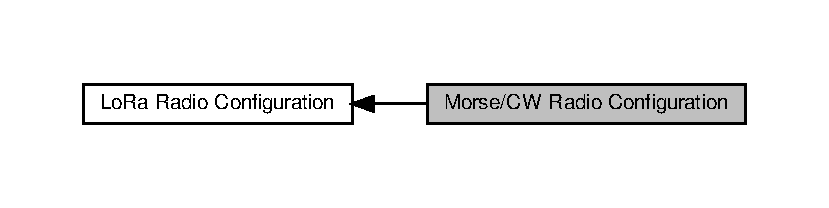
\includegraphics[width=350pt]{group__defines__radio__morse__cw__configuration}
\end{center}
\end{figure}
\subsection*{Macros}
\begin{DoxyCompactItemize}
\item 
\#define \hyperlink{group__defines__radio__morse__cw__configuration_gaae7df1e5ab7ea07920fef2cc9456cbdd}{N\+U\+M\+\_\+\+C\+W\+\_\+\+B\+E\+E\+PS}~3
\item 
\#define \hyperlink{group__defines__radio__morse__cw__configuration_ga7713a1dd2dd939f0314fb6abf067deb5}{M\+O\+R\+S\+E\+\_\+\+P\+R\+E\+A\+M\+B\+L\+E\+\_\+\+L\+E\+N\+G\+TH}~0
\item 
\#define \hyperlink{group__defines__radio__morse__cw__configuration_ga7ecb6f014f236823544c51e3d9d43c30}{M\+O\+R\+S\+E\+\_\+\+S\+P\+E\+ED}~20
\item 
\#define \hyperlink{group__defines__radio__morse__cw__configuration_ga4573c7b1d2f3cdaddadb3fe7aae6de6f}{M\+O\+R\+S\+E\+\_\+\+B\+A\+T\+T\+E\+R\+Y\+\_\+\+M\+IN}~3.\+2
\item 
\#define \hyperlink{group__defines__radio__morse__cw__configuration_ga2d1e75f9b5a4f4217800b4cc91f2bcbb}{M\+O\+R\+S\+E\+\_\+\+B\+A\+T\+T\+E\+R\+Y\+\_\+\+S\+T\+EP}~0.\+05
\item 
\#define \hyperlink{group__defines__radio__morse__cw__configuration_gab3651b3dc8b84b12fe86ec9a8a9aaaae}{M\+O\+R\+S\+E\+\_\+\+B\+E\+A\+C\+O\+N\+\_\+\+L\+O\+O\+P\+\_\+\+F\+R\+EQ}~2
\end{DoxyCompactItemize}


\subsection{Detailed Description}
\begin{DoxyRefDesc}{Test}
\item[\hyperlink{test__test000029}{Test}](ID C\+O\+N\+F\+\_\+\+M\+O\+R\+S\+E\+\_\+\+C\+W\+\_\+\+T0) (S\+EV 1) Check that the number of beeps given by the radio in low power mode is N\+U\+M\+\_\+\+C\+W\+\_\+\+B\+E\+E\+PS. 

(ID C\+O\+N\+F\+\_\+\+M\+O\+R\+S\+E\+\_\+\+C\+W\+\_\+\+T1) (S\+EV 1) Check that the morse starts a signal with M\+O\+R\+S\+E\+\_\+\+P\+R\+E\+A\+M\+B\+L\+E\+\_\+\+L\+E\+N\+G\+TH. 

(ID C\+O\+N\+F\+\_\+\+M\+O\+R\+S\+E\+\_\+\+C\+W\+\_\+\+T2) (S\+EV 1) Check that the words per minute of the morse transmissions is M\+O\+R\+S\+E\+\_\+\+S\+P\+E\+ED.\end{DoxyRefDesc}


\subsection{Macro Definition Documentation}
\mbox{\Hypertarget{group__defines__radio__morse__cw__configuration_ga4573c7b1d2f3cdaddadb3fe7aae6de6f}\label{group__defines__radio__morse__cw__configuration_ga4573c7b1d2f3cdaddadb3fe7aae6de6f}} 
\index{Morse/\+C\+W Radio Configuration@{Morse/\+C\+W Radio Configuration}!M\+O\+R\+S\+E\+\_\+\+B\+A\+T\+T\+E\+R\+Y\+\_\+\+M\+IN@{M\+O\+R\+S\+E\+\_\+\+B\+A\+T\+T\+E\+R\+Y\+\_\+\+M\+IN}}
\index{M\+O\+R\+S\+E\+\_\+\+B\+A\+T\+T\+E\+R\+Y\+\_\+\+M\+IN@{M\+O\+R\+S\+E\+\_\+\+B\+A\+T\+T\+E\+R\+Y\+\_\+\+M\+IN}!Morse/\+C\+W Radio Configuration@{Morse/\+C\+W Radio Configuration}}
\subsubsection{\texorpdfstring{M\+O\+R\+S\+E\+\_\+\+B\+A\+T\+T\+E\+R\+Y\+\_\+\+M\+IN}{MORSE\_BATTERY\_MIN}}
{\footnotesize\ttfamily \#define M\+O\+R\+S\+E\+\_\+\+B\+A\+T\+T\+E\+R\+Y\+\_\+\+M\+IN~3.\+2}

minimum voltage value that can be send via Morse (corresponds to \textquotesingle{}A\textquotesingle{}), volts 

Definition at line 567 of file configuration.\+h.

\mbox{\Hypertarget{group__defines__radio__morse__cw__configuration_ga2d1e75f9b5a4f4217800b4cc91f2bcbb}\label{group__defines__radio__morse__cw__configuration_ga2d1e75f9b5a4f4217800b4cc91f2bcbb}} 
\index{Morse/\+C\+W Radio Configuration@{Morse/\+C\+W Radio Configuration}!M\+O\+R\+S\+E\+\_\+\+B\+A\+T\+T\+E\+R\+Y\+\_\+\+S\+T\+EP@{M\+O\+R\+S\+E\+\_\+\+B\+A\+T\+T\+E\+R\+Y\+\_\+\+S\+T\+EP}}
\index{M\+O\+R\+S\+E\+\_\+\+B\+A\+T\+T\+E\+R\+Y\+\_\+\+S\+T\+EP@{M\+O\+R\+S\+E\+\_\+\+B\+A\+T\+T\+E\+R\+Y\+\_\+\+S\+T\+EP}!Morse/\+C\+W Radio Configuration@{Morse/\+C\+W Radio Configuration}}
\subsubsection{\texorpdfstring{M\+O\+R\+S\+E\+\_\+\+B\+A\+T\+T\+E\+R\+Y\+\_\+\+S\+T\+EP}{MORSE\_BATTERY\_STEP}}
{\footnotesize\ttfamily \#define M\+O\+R\+S\+E\+\_\+\+B\+A\+T\+T\+E\+R\+Y\+\_\+\+S\+T\+EP~0.\+05}

voltage step in Morse, volts 

Definition at line 568 of file configuration.\+h.

\mbox{\Hypertarget{group__defines__radio__morse__cw__configuration_gab3651b3dc8b84b12fe86ec9a8a9aaaae}\label{group__defines__radio__morse__cw__configuration_gab3651b3dc8b84b12fe86ec9a8a9aaaae}} 
\index{Morse/\+C\+W Radio Configuration@{Morse/\+C\+W Radio Configuration}!M\+O\+R\+S\+E\+\_\+\+B\+E\+A\+C\+O\+N\+\_\+\+L\+O\+O\+P\+\_\+\+F\+R\+EQ@{M\+O\+R\+S\+E\+\_\+\+B\+E\+A\+C\+O\+N\+\_\+\+L\+O\+O\+P\+\_\+\+F\+R\+EQ}}
\index{M\+O\+R\+S\+E\+\_\+\+B\+E\+A\+C\+O\+N\+\_\+\+L\+O\+O\+P\+\_\+\+F\+R\+EQ@{M\+O\+R\+S\+E\+\_\+\+B\+E\+A\+C\+O\+N\+\_\+\+L\+O\+O\+P\+\_\+\+F\+R\+EQ}!Morse/\+C\+W Radio Configuration@{Morse/\+C\+W Radio Configuration}}
\subsubsection{\texorpdfstring{M\+O\+R\+S\+E\+\_\+\+B\+E\+A\+C\+O\+N\+\_\+\+L\+O\+O\+P\+\_\+\+F\+R\+EQ}{MORSE\_BEACON\_LOOP\_FREQ}}
{\footnotesize\ttfamily \#define M\+O\+R\+S\+E\+\_\+\+B\+E\+A\+C\+O\+N\+\_\+\+L\+O\+O\+P\+\_\+\+F\+R\+EQ~2}

how often to transmit full Morse code beacon (e.\+g. transmit every second main loop when set to 2) 

Definition at line 569 of file configuration.\+h.

\mbox{\Hypertarget{group__defines__radio__morse__cw__configuration_ga7713a1dd2dd939f0314fb6abf067deb5}\label{group__defines__radio__morse__cw__configuration_ga7713a1dd2dd939f0314fb6abf067deb5}} 
\index{Morse/\+C\+W Radio Configuration@{Morse/\+C\+W Radio Configuration}!M\+O\+R\+S\+E\+\_\+\+P\+R\+E\+A\+M\+B\+L\+E\+\_\+\+L\+E\+N\+G\+TH@{M\+O\+R\+S\+E\+\_\+\+P\+R\+E\+A\+M\+B\+L\+E\+\_\+\+L\+E\+N\+G\+TH}}
\index{M\+O\+R\+S\+E\+\_\+\+P\+R\+E\+A\+M\+B\+L\+E\+\_\+\+L\+E\+N\+G\+TH@{M\+O\+R\+S\+E\+\_\+\+P\+R\+E\+A\+M\+B\+L\+E\+\_\+\+L\+E\+N\+G\+TH}!Morse/\+C\+W Radio Configuration@{Morse/\+C\+W Radio Configuration}}
\subsubsection{\texorpdfstring{M\+O\+R\+S\+E\+\_\+\+P\+R\+E\+A\+M\+B\+L\+E\+\_\+\+L\+E\+N\+G\+TH}{MORSE\_PREAMBLE\_LENGTH}}
{\footnotesize\ttfamily \#define M\+O\+R\+S\+E\+\_\+\+P\+R\+E\+A\+M\+B\+L\+E\+\_\+\+L\+E\+N\+G\+TH~0}

number of start signal repetitions 

Definition at line 565 of file configuration.\+h.

\mbox{\Hypertarget{group__defines__radio__morse__cw__configuration_ga7ecb6f014f236823544c51e3d9d43c30}\label{group__defines__radio__morse__cw__configuration_ga7ecb6f014f236823544c51e3d9d43c30}} 
\index{Morse/\+C\+W Radio Configuration@{Morse/\+C\+W Radio Configuration}!M\+O\+R\+S\+E\+\_\+\+S\+P\+E\+ED@{M\+O\+R\+S\+E\+\_\+\+S\+P\+E\+ED}}
\index{M\+O\+R\+S\+E\+\_\+\+S\+P\+E\+ED@{M\+O\+R\+S\+E\+\_\+\+S\+P\+E\+ED}!Morse/\+C\+W Radio Configuration@{Morse/\+C\+W Radio Configuration}}
\subsubsection{\texorpdfstring{M\+O\+R\+S\+E\+\_\+\+S\+P\+E\+ED}{MORSE\_SPEED}}
{\footnotesize\ttfamily \#define M\+O\+R\+S\+E\+\_\+\+S\+P\+E\+ED~20}

words per minute 

Definition at line 566 of file configuration.\+h.

\mbox{\Hypertarget{group__defines__radio__morse__cw__configuration_gaae7df1e5ab7ea07920fef2cc9456cbdd}\label{group__defines__radio__morse__cw__configuration_gaae7df1e5ab7ea07920fef2cc9456cbdd}} 
\index{Morse/\+C\+W Radio Configuration@{Morse/\+C\+W Radio Configuration}!N\+U\+M\+\_\+\+C\+W\+\_\+\+B\+E\+E\+PS@{N\+U\+M\+\_\+\+C\+W\+\_\+\+B\+E\+E\+PS}}
\index{N\+U\+M\+\_\+\+C\+W\+\_\+\+B\+E\+E\+PS@{N\+U\+M\+\_\+\+C\+W\+\_\+\+B\+E\+E\+PS}!Morse/\+C\+W Radio Configuration@{Morse/\+C\+W Radio Configuration}}
\subsubsection{\texorpdfstring{N\+U\+M\+\_\+\+C\+W\+\_\+\+B\+E\+E\+PS}{NUM\_CW\_BEEPS}}
{\footnotesize\ttfamily \#define N\+U\+M\+\_\+\+C\+W\+\_\+\+B\+E\+E\+PS~3}

number of CW sync beeps in low power mode 

Definition at line 564 of file configuration.\+h.


\hypertarget{group__defines__radio__modem__configuration}{}\section{Modem Identifiers}
\label{group__defines__radio__modem__configuration}\index{Modem Identifiers@{Modem Identifiers}}
Collaboration diagram for Modem Identifiers\+:
\nopagebreak
\begin{figure}[H]
\begin{center}
\leavevmode
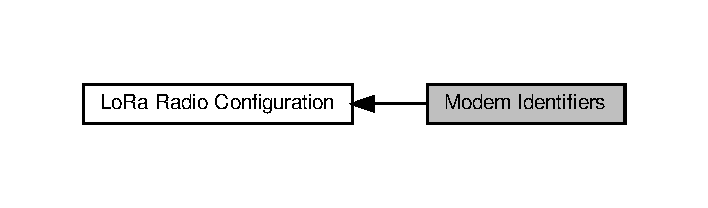
\includegraphics[width=340pt]{group__defines__radio__modem__configuration}
\end{center}
\end{figure}
\subsection*{Macros}
\begin{DoxyCompactItemize}
\item 
\mbox{\Hypertarget{group__defines__radio__modem__configuration_ga4214cb338675365d6e2e14fb1f8436d7}\label{group__defines__radio__modem__configuration_ga4214cb338675365d6e2e14fb1f8436d7}} 
\#define {\bfseries M\+O\+D\+E\+M\+\_\+\+L\+O\+RA}~\textquotesingle{}L\textquotesingle{}
\item 
\mbox{\Hypertarget{group__defines__radio__modem__configuration_ga8b344b5ca597731ca0ccabcdee4a24a2}\label{group__defines__radio__modem__configuration_ga8b344b5ca597731ca0ccabcdee4a24a2}} 
\#define {\bfseries M\+O\+D\+E\+M\+\_\+\+F\+SK}~\textquotesingle{}F\textquotesingle{}
\end{DoxyCompactItemize}


\subsection{Detailed Description}
\begin{DoxyRefDesc}{Test}
\item[\hyperlink{test__test000030}{Test}](ID C\+O\+N\+F\+\_\+\+M\+O\+D\+E\+M\+\_\+\+T0) Check that M\+O\+D\+E\+M\+\_\+\+L\+O\+RA is suitable. 

(ID C\+O\+N\+F\+\_\+\+M\+O\+D\+E\+M\+\_\+\+T1) Check that M\+O\+D\+E\+M\+\_\+\+F\+SK is suitable.\end{DoxyRefDesc}

\hypertarget{group__defines__global__variables}{}\section{Global Variables}
\label{group__defines__global__variables}\index{Global Variables@{Global Variables}}
Collaboration diagram for Global Variables\+:
\nopagebreak
\begin{figure}[H]
\begin{center}
\leavevmode
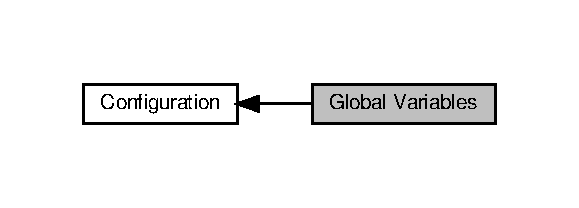
\includegraphics[width=278pt]{group__defines__global__variables}
\end{center}
\end{figure}
\subsection*{Variables}
\begin{DoxyCompactItemize}
\item 
volatile bool \hyperlink{group__defines__global__variables_gac4e4a006083dd62a0a607861795b74ad}{interrupts\+Enabled}
\item 
volatile bool \hyperlink{group__defines__global__variables_ga9caaf5e68386ab1a12ef35bee230b1f2}{data\+Received}
\item 
uint8\+\_\+t \hyperlink{group__defines__global__variables_ga3ff59835e905207ccc63426c658ef705}{current\+Modem}
\item 
uint8\+\_\+t \hyperlink{group__defines__global__variables_ga1b7f588d9dfbb3b5e8553ce78dacac8d}{spreading\+Factor\+Mode}
\item 
uint32\+\_\+t \hyperlink{group__defines__global__variables_gad3d1c7107632ee3536eb442026fe08fa}{last\+Heartbeat}
\item 
I\+N\+A226 \hyperlink{group__defines__global__variables_gabef7273c58516662eed53fda518d0eaa}{ina}
\item 
S\+X1268 \hyperlink{group__defines__global__variables_ga4d67d9af4c43901b2f5171b55270e4f7}{radio}
\item 
Morse\+Client \hyperlink{group__defines__global__variables_gad7b71738b4bf5134ae10234ed8dee889}{morse}
\item 
const char $\ast$ \hyperlink{group__defines__global__variables_gaa4a2ebcb494493f648ae1e6975672575}{password}
\item 
const uint8\+\_\+t \hyperlink{group__defines__global__variables_ga2623c5901f38974be6d0186e14cbcfa7}{encryption\+Key} \mbox{[}$\,$\mbox{]}
\end{DoxyCompactItemize}


\subsection{Detailed Description}


\subsection{Variable Documentation}
\mbox{\Hypertarget{group__defines__global__variables_ga3ff59835e905207ccc63426c658ef705}\label{group__defines__global__variables_ga3ff59835e905207ccc63426c658ef705}} 
\index{Global Variables@{Global Variables}!current\+Modem@{current\+Modem}}
\index{current\+Modem@{current\+Modem}!Global Variables@{Global Variables}}
\subsubsection{\texorpdfstring{current\+Modem}{currentModem}}
{\footnotesize\ttfamily uint8\+\_\+t current\+Modem}

Current modem configuration. 

Definition at line 10 of file configuration.\+cpp.

\mbox{\Hypertarget{group__defines__global__variables_ga9caaf5e68386ab1a12ef35bee230b1f2}\label{group__defines__global__variables_ga9caaf5e68386ab1a12ef35bee230b1f2}} 
\index{Global Variables@{Global Variables}!data\+Received@{data\+Received}}
\index{data\+Received@{data\+Received}!Global Variables@{Global Variables}}
\subsubsection{\texorpdfstring{data\+Received}{dataReceived}}
{\footnotesize\ttfamily volatile bool data\+Received}

Flag to signal data was received from I\+SR. 

Definition at line 7 of file configuration.\+cpp.

\mbox{\Hypertarget{group__defines__global__variables_ga2623c5901f38974be6d0186e14cbcfa7}\label{group__defines__global__variables_ga2623c5901f38974be6d0186e14cbcfa7}} 
\index{Global Variables@{Global Variables}!encryption\+Key@{encryption\+Key}}
\index{encryption\+Key@{encryption\+Key}!Global Variables@{Global Variables}}
\subsubsection{\texorpdfstring{encryption\+Key}{encryptionKey}}
{\footnotesize\ttfamily const uint8\+\_\+t encryption\+Key\mbox{[}$\,$\mbox{]}}

Encryption key (A\+ES). 

Definition at line 29 of file configuration.\+cpp.

\mbox{\Hypertarget{group__defines__global__variables_gabef7273c58516662eed53fda518d0eaa}\label{group__defines__global__variables_gabef7273c58516662eed53fda518d0eaa}} 
\index{Global Variables@{Global Variables}!ina@{ina}}
\index{ina@{ina}!Global Variables@{Global Variables}}
\subsubsection{\texorpdfstring{ina}{ina}}
{\footnotesize\ttfamily I\+N\+A226 ina}

I\+N\+A226 object. 

Definition at line 19 of file configuration.\+cpp.

\mbox{\Hypertarget{group__defines__global__variables_gac4e4a006083dd62a0a607861795b74ad}\label{group__defines__global__variables_gac4e4a006083dd62a0a607861795b74ad}} 
\index{Global Variables@{Global Variables}!interrupts\+Enabled@{interrupts\+Enabled}}
\index{interrupts\+Enabled@{interrupts\+Enabled}!Global Variables@{Global Variables}}
\subsubsection{\texorpdfstring{interrupts\+Enabled}{interruptsEnabled}}
{\footnotesize\ttfamily volatile bool interrupts\+Enabled}

Flag to signal interrupts enabled/disabled. 

Definition at line 4 of file configuration.\+cpp.

\mbox{\Hypertarget{group__defines__global__variables_gad3d1c7107632ee3536eb442026fe08fa}\label{group__defines__global__variables_gad3d1c7107632ee3536eb442026fe08fa}} 
\index{Global Variables@{Global Variables}!last\+Heartbeat@{last\+Heartbeat}}
\index{last\+Heartbeat@{last\+Heartbeat}!Global Variables@{Global Variables}}
\subsubsection{\texorpdfstring{last\+Heartbeat}{lastHeartbeat}}
{\footnotesize\ttfamily uint32\+\_\+t last\+Heartbeat}

Timestamp for the watchdog. 

Definition at line 16 of file configuration.\+cpp.

\mbox{\Hypertarget{group__defines__global__variables_gad7b71738b4bf5134ae10234ed8dee889}\label{group__defines__global__variables_gad7b71738b4bf5134ae10234ed8dee889}} 
\index{Global Variables@{Global Variables}!morse@{morse}}
\index{morse@{morse}!Global Variables@{Global Variables}}
\subsubsection{\texorpdfstring{morse}{morse}}
{\footnotesize\ttfamily Morse\+Client morse}

Morse\+Client object. \mbox{\Hypertarget{group__defines__global__variables_gaa4a2ebcb494493f648ae1e6975672575}\label{group__defines__global__variables_gaa4a2ebcb494493f648ae1e6975672575}} 
\index{Global Variables@{Global Variables}!password@{password}}
\index{password@{password}!Global Variables@{Global Variables}}
\subsubsection{\texorpdfstring{password}{password}}
{\footnotesize\ttfamily const char$\ast$ password}

Transmission password (A\+ES). 

Definition at line 26 of file configuration.\+cpp.

\mbox{\Hypertarget{group__defines__global__variables_ga4d67d9af4c43901b2f5171b55270e4f7}\label{group__defines__global__variables_ga4d67d9af4c43901b2f5171b55270e4f7}} 
\index{Global Variables@{Global Variables}!radio@{radio}}
\index{radio@{radio}!Global Variables@{Global Variables}}
\subsubsection{\texorpdfstring{radio}{radio}}
{\footnotesize\ttfamily S\+X1268 radio}

S\+X1268 object. 

Definition at line 22 of file configuration.\+cpp.

\mbox{\Hypertarget{group__defines__global__variables_ga1b7f588d9dfbb3b5e8553ce78dacac8d}\label{group__defines__global__variables_ga1b7f588d9dfbb3b5e8553ce78dacac8d}} 
\index{Global Variables@{Global Variables}!spreading\+Factor\+Mode@{spreading\+Factor\+Mode}}
\index{spreading\+Factor\+Mode@{spreading\+Factor\+Mode}!Global Variables@{Global Variables}}
\subsubsection{\texorpdfstring{spreading\+Factor\+Mode}{spreadingFactorMode}}
{\footnotesize\ttfamily uint8\+\_\+t spreading\+Factor\+Mode}

Current spreading factor mode. 

Definition at line 13 of file configuration.\+cpp.


\hypertarget{group__debugging__h__defines}{}\section{Debugging Utility}
\label{group__debugging__h__defines}\index{Debugging Utility@{Debugging Utility}}
\subsection*{Macros}
\begin{DoxyCompactItemize}
\item 
\mbox{\Hypertarget{group__debugging__h__defines_gac2c7820060c166dde1fb4ee57949e16f}\label{group__debugging__h__defines_gac2c7820060c166dde1fb4ee57949e16f}} 
\#define {\bfseries F\+O\+S\+S\+A\+S\+A\+T\+\_\+\+D\+E\+B\+UG}
\item 
\mbox{\Hypertarget{group__debugging__h__defines_ga01c1d95ee747390a841f87529ca6eda1}\label{group__debugging__h__defines_ga01c1d95ee747390a841f87529ca6eda1}} 
\#define {\bfseries F\+O\+S\+S\+A\+S\+A\+T\+\_\+\+D\+E\+B\+U\+G\+\_\+\+P\+O\+RT}~Serial
\item 
\mbox{\Hypertarget{group__debugging__h__defines_ga222f840c0273a7c14b37d689ba45501c}\label{group__debugging__h__defines_ga222f840c0273a7c14b37d689ba45501c}} 
\#define {\bfseries F\+O\+S\+S\+A\+S\+A\+T\+\_\+\+D\+E\+B\+U\+G\+\_\+\+S\+P\+E\+ED}~115200
\item 
\mbox{\Hypertarget{group__debugging__h__defines_ga08e005173cbb2de7f1ed6fae03cedf9f}\label{group__debugging__h__defines_ga08e005173cbb2de7f1ed6fae03cedf9f}} 
\#define {\bfseries F\+O\+S\+S\+A\+S\+A\+T\+\_\+\+D\+E\+B\+U\+G\+\_\+\+B\+E\+G\+IN}(...)~\{ F\+O\+S\+S\+A\+S\+A\+T\+\_\+\+D\+E\+B\+U\+G\+\_\+\+P\+O\+R\+T.\+begin(\+\_\+\+\_\+\+V\+A\+\_\+\+A\+R\+G\+S\+\_\+\+\_\+); \}
\item 
\mbox{\Hypertarget{group__debugging__h__defines_gaa825f0c9ffcfeff331d7843ba749a104}\label{group__debugging__h__defines_gaa825f0c9ffcfeff331d7843ba749a104}} 
\#define {\bfseries F\+O\+S\+S\+A\+S\+A\+T\+\_\+\+D\+E\+B\+U\+G\+\_\+\+P\+R\+I\+NT}(...)~\{ F\+O\+S\+S\+A\+S\+A\+T\+\_\+\+D\+E\+B\+U\+G\+\_\+\+P\+O\+R\+T.\+print(\+\_\+\+\_\+\+V\+A\+\_\+\+A\+R\+G\+S\+\_\+\+\_\+); \}
\item 
\mbox{\Hypertarget{group__debugging__h__defines_ga065c558f3c794981a1a217f5382226ab}\label{group__debugging__h__defines_ga065c558f3c794981a1a217f5382226ab}} 
\#define {\bfseries F\+O\+S\+S\+A\+S\+A\+T\+\_\+\+D\+E\+B\+U\+G\+\_\+\+P\+R\+I\+N\+T\+LN}(...)~\{ F\+O\+S\+S\+A\+S\+A\+T\+\_\+\+D\+E\+B\+U\+G\+\_\+\+P\+O\+R\+T.\+println(\+\_\+\+\_\+\+V\+A\+\_\+\+A\+R\+G\+S\+\_\+\+\_\+); \}
\item 
\mbox{\Hypertarget{group__debugging__h__defines_gafa6e3f728aa852ff94bfddfa91a691c4}\label{group__debugging__h__defines_gafa6e3f728aa852ff94bfddfa91a691c4}} 
\#define {\bfseries F\+O\+S\+S\+A\+S\+A\+T\+\_\+\+D\+E\+B\+U\+G\+\_\+\+W\+R\+I\+TE}(...)~\{ F\+O\+S\+S\+A\+S\+A\+T\+\_\+\+D\+E\+B\+U\+G\+\_\+\+P\+O\+R\+T.\+write(\+\_\+\+\_\+\+V\+A\+\_\+\+A\+R\+G\+S\+\_\+\+\_\+); \}
\item 
\#define {\bfseries F\+O\+S\+S\+A\+S\+A\+T\+\_\+\+D\+E\+B\+U\+G\+\_\+\+P\+R\+I\+N\+T\+\_\+\+B\+U\+FF}(B\+U\+FF,  L\+EN)
\item 
\#define {\bfseries F\+O\+S\+S\+A\+S\+A\+T\+\_\+\+D\+E\+B\+U\+G\+\_\+\+P\+R\+I\+N\+T\+\_\+\+E\+E\+P\+R\+OM}(A\+D\+DR,  L\+EN)
\item 
\mbox{\Hypertarget{group__debugging__h__defines_ga8ac2aabe99ce81a792a84a66592710cb}\label{group__debugging__h__defines_ga8ac2aabe99ce81a792a84a66592710cb}} 
\#define {\bfseries F\+O\+S\+S\+A\+S\+A\+T\+\_\+\+D\+E\+B\+U\+G\+\_\+\+D\+E\+L\+AY}(MS)~\{ delay(MS); \}
\item 
\mbox{\Hypertarget{group__debugging__h__defines_ga0e3ff23c7e08ddcb70e0d68767603b6d}\label{group__debugging__h__defines_ga0e3ff23c7e08ddcb70e0d68767603b6d}} 
\#define {\bfseries F\+O\+S\+S\+A\+S\+A\+T\+\_\+\+V\+E\+R\+B\+O\+S\+E\+\_\+\+P\+R\+I\+NT}(...)~\{\}
\item 
\mbox{\Hypertarget{group__debugging__h__defines_ga65c0457bb68ebc5be2ad7240b8176cf4}\label{group__debugging__h__defines_ga65c0457bb68ebc5be2ad7240b8176cf4}} 
\#define {\bfseries F\+O\+S\+S\+A\+S\+A\+T\+\_\+\+V\+E\+R\+B\+O\+S\+E\+\_\+\+P\+R\+I\+N\+T\+LN}(...)~\{\}
\end{DoxyCompactItemize}


\subsection{Detailed Description}


\subsection{Macro Definition Documentation}
\mbox{\Hypertarget{group__debugging__h__defines_ga527ce33164864ab76091954433aff62b}\label{group__debugging__h__defines_ga527ce33164864ab76091954433aff62b}} 
\index{Debugging Utility@{Debugging Utility}!F\+O\+S\+S\+A\+S\+A\+T\+\_\+\+D\+E\+B\+U\+G\+\_\+\+P\+R\+I\+N\+T\+\_\+\+B\+U\+FF@{F\+O\+S\+S\+A\+S\+A\+T\+\_\+\+D\+E\+B\+U\+G\+\_\+\+P\+R\+I\+N\+T\+\_\+\+B\+U\+FF}}
\index{F\+O\+S\+S\+A\+S\+A\+T\+\_\+\+D\+E\+B\+U\+G\+\_\+\+P\+R\+I\+N\+T\+\_\+\+B\+U\+FF@{F\+O\+S\+S\+A\+S\+A\+T\+\_\+\+D\+E\+B\+U\+G\+\_\+\+P\+R\+I\+N\+T\+\_\+\+B\+U\+FF}!Debugging Utility@{Debugging Utility}}
\subsubsection{\texorpdfstring{F\+O\+S\+S\+A\+S\+A\+T\+\_\+\+D\+E\+B\+U\+G\+\_\+\+P\+R\+I\+N\+T\+\_\+\+B\+U\+FF}{FOSSASAT\_DEBUG\_PRINT\_BUFF}}
{\footnotesize\ttfamily \#define F\+O\+S\+S\+A\+S\+A\+T\+\_\+\+D\+E\+B\+U\+G\+\_\+\+P\+R\+I\+N\+T\+\_\+\+B\+U\+FF(\begin{DoxyParamCaption}\item[{}]{B\+U\+FF,  }\item[{}]{L\+EN }\end{DoxyParamCaption})}

{\bfseries Value\+:}
\begin{DoxyCode}
\{ \(\backslash\)
    for(\textcolor{keywordtype}{size\_t} i = 0; i < LEN; i++) \{ \(\backslash\)
      FOSSASAT\_DEBUG\_PORT.print(F(\textcolor{stringliteral}{"0x"})); \(\backslash\)
      FOSSASAT\_DEBUG\_PORT.print(BUFF[i], HEX); \(\backslash\)
      FOSSASAT\_DEBUG\_PORT.print(\textcolor{charliteral}{'\(\backslash\)t'}); \(\backslash\)
      FOSSASAT\_DEBUG\_PORT.write(BUFF[i]); \(\backslash\)
      FOSSASAT\_DEBUG\_PORT.println(); \(\backslash\)
    \} \}
\end{DoxyCode}


Definition at line 30 of file debugging\+\_\+utilities.\+h.

\mbox{\Hypertarget{group__debugging__h__defines_ga70024289d51d1a6100dbee95b5f7d49a}\label{group__debugging__h__defines_ga70024289d51d1a6100dbee95b5f7d49a}} 
\index{Debugging Utility@{Debugging Utility}!F\+O\+S\+S\+A\+S\+A\+T\+\_\+\+D\+E\+B\+U\+G\+\_\+\+P\+R\+I\+N\+T\+\_\+\+E\+E\+P\+R\+OM@{F\+O\+S\+S\+A\+S\+A\+T\+\_\+\+D\+E\+B\+U\+G\+\_\+\+P\+R\+I\+N\+T\+\_\+\+E\+E\+P\+R\+OM}}
\index{F\+O\+S\+S\+A\+S\+A\+T\+\_\+\+D\+E\+B\+U\+G\+\_\+\+P\+R\+I\+N\+T\+\_\+\+E\+E\+P\+R\+OM@{F\+O\+S\+S\+A\+S\+A\+T\+\_\+\+D\+E\+B\+U\+G\+\_\+\+P\+R\+I\+N\+T\+\_\+\+E\+E\+P\+R\+OM}!Debugging Utility@{Debugging Utility}}
\subsubsection{\texorpdfstring{F\+O\+S\+S\+A\+S\+A\+T\+\_\+\+D\+E\+B\+U\+G\+\_\+\+P\+R\+I\+N\+T\+\_\+\+E\+E\+P\+R\+OM}{FOSSASAT\_DEBUG\_PRINT\_EEPROM}}
{\footnotesize\ttfamily \#define F\+O\+S\+S\+A\+S\+A\+T\+\_\+\+D\+E\+B\+U\+G\+\_\+\+P\+R\+I\+N\+T\+\_\+\+E\+E\+P\+R\+OM(\begin{DoxyParamCaption}\item[{}]{A\+D\+DR,  }\item[{}]{L\+EN }\end{DoxyParamCaption})}

{\bfseries Value\+:}
\begin{DoxyCode}
\{ \(\backslash\)
    uint8\_t readBuff[0xFF]; \(\backslash\)
    char buff[16]; \(\backslash\)
    if(LEN < 16) \{ \(\backslash\)
      for(uint8\_t i = 0; i < LEN; i++) \{ \(\backslash\)
        sprintf(buff, \textcolor{stringliteral}{"%02x "}, EEPROM.read(ADDR + i)); \(\backslash\)
        FOSSASAT\_DEBUG\_PORT.print(buff); \(\backslash\)
      \} \(\backslash\)
      FOSSASAT\_DEBUG\_PORT.println(); \(\backslash\)
    \} \textcolor{keywordflow}{else} \{ \(\backslash\)
      for(\textcolor{keywordtype}{size\_t} i = 0; i < LEN/16; i++) \{ \(\backslash\)
        for(uint8\_t j = 0; j < 16; j++) \{ \(\backslash\)
          sprintf(buff, \textcolor{stringliteral}{"%02x "}, EEPROM.read(ADDR + i*16 + j)); \(\backslash\)
          FOSSASAT\_DEBUG\_PORT.print(buff); \(\backslash\)
        \} \(\backslash\)
        FOSSASAT\_DEBUG\_PORT.println(); \(\backslash\)
      \} \(\backslash\)
    \} \}
\end{DoxyCode}


Definition at line 38 of file debugging\+\_\+utilities.\+h.


\chapter{Data Structure Documentation}
\hypertarget{unionpower_config__t}{}\section{power\+Config\+\_\+t Union Reference}
\label{unionpower_config__t}\index{power\+Config\+\_\+t@{power\+Config\+\_\+t}}


Union to quickly access power configuration bits or the entire single-\/byte value.  




{\ttfamily \#include $<$power\+\_\+control.\+h$>$}



Collaboration diagram for power\+Config\+\_\+t\+:
\nopagebreak
\begin{figure}[H]
\begin{center}
\leavevmode
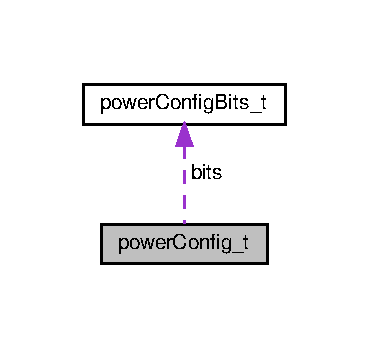
\includegraphics[width=177pt]{unionpower_config__t__coll__graph}
\end{center}
\end{figure}
\subsection*{Data Fields}
\begin{DoxyCompactItemize}
\item 
\mbox{\Hypertarget{unionpower_config__t_a4d894bc56a0a7c9fbb405955f799ee46}\label{unionpower_config__t_a4d894bc56a0a7c9fbb405955f799ee46}} 
struct \hyperlink{structpower_config_bits__t}{power\+Config\+Bits\+\_\+t} {\bfseries bits}
\item 
\mbox{\Hypertarget{unionpower_config__t_a8c7fe6eb17488063a0393bc90231f090}\label{unionpower_config__t_a8c7fe6eb17488063a0393bc90231f090}} 
uint8\+\_\+t {\bfseries val}
\end{DoxyCompactItemize}


\subsection{Detailed Description}
Union to quickly access power configuration bits or the entire single-\/byte value. 

Definition at line 26 of file power\+\_\+control.\+h.



The documentation for this union was generated from the following file\+:\begin{DoxyCompactItemize}
\item 
Fossa\+Sat1\+B/\hyperlink{power__control_8h}{power\+\_\+control.\+h}\end{DoxyCompactItemize}

\hypertarget{structpower_config_bits__t}{}\section{power\+Config\+Bits\+\_\+t Struct Reference}
\label{structpower_config_bits__t}\index{power\+Config\+Bits\+\_\+t@{power\+Config\+Bits\+\_\+t}}


Power configuration strutcture, each entry is one bit long. Total 1 byte, low\+Power\+Mode\+Active is the least significant bit.  




{\ttfamily \#include $<$power\+\_\+control.\+h$>$}

\subsection*{Data Fields}
\begin{DoxyCompactItemize}
\item 
\mbox{\Hypertarget{structpower_config_bits__t_aee72a13a91270d9fa387524b1d92dff8}\label{structpower_config_bits__t_aee72a13a91270d9fa387524b1d92dff8}} 
uint8\+\_\+t {\bfseries low\+Power\+Mode\+Active}\+: 1
\item 
\mbox{\Hypertarget{structpower_config_bits__t_a3f4d8faa57c2a6bfbbfb3e7771e4c73b}\label{structpower_config_bits__t_a3f4d8faa57c2a6bfbbfb3e7771e4c73b}} 
uint8\+\_\+t {\bfseries low\+Power\+Mode\+Enabled}\+: 1
\item 
\mbox{\Hypertarget{structpower_config_bits__t_ad16350358127656cb4e94755923e6b96}\label{structpower_config_bits__t_ad16350358127656cb4e94755923e6b96}} 
uint8\+\_\+t {\bfseries mppt\+Temp\+Switch\+Enabled}\+: 1
\item 
\mbox{\Hypertarget{structpower_config_bits__t_aad7dea2284fd52c9900003dabaf950c6}\label{structpower_config_bits__t_aad7dea2284fd52c9900003dabaf950c6}} 
uint8\+\_\+t {\bfseries mppt\+Keep\+Alive\+Enabled}\+: 1
\item 
\mbox{\Hypertarget{structpower_config_bits__t_a6b88402c62ae43ff15edf6e38997178a}\label{structpower_config_bits__t_a6b88402c62ae43ff15edf6e38997178a}} 
uint8\+\_\+t {\bfseries transmit\+Enabled}\+: 1
\end{DoxyCompactItemize}


\subsection{Detailed Description}
Power configuration strutcture, each entry is one bit long. Total 1 byte, low\+Power\+Mode\+Active is the least significant bit. 

Definition at line 15 of file power\+\_\+control.\+h.



The documentation for this struct was generated from the following file\+:\begin{DoxyCompactItemize}
\item 
Fossa\+Sat1\+B/\hyperlink{power__control_8h}{power\+\_\+control.\+h}\end{DoxyCompactItemize}

\chapter{File Documentation}
\hypertarget{communication_8h}{}\section{Fossa\+Sat1\+B/communication.h File Reference}
\label{communication_8h}\index{Fossa\+Sat1\+B/communication.\+h@{Fossa\+Sat1\+B/communication.\+h}}


This system is the main interface that is used to transmit message, configure the radio and process received transmissions.  


{\ttfamily \#include \char`\"{}Fossa\+Sat1\+B.\+h\char`\"{}}\newline
Include dependency graph for communication.\+h\+:
\nopagebreak
\begin{figure}[H]
\begin{center}
\leavevmode
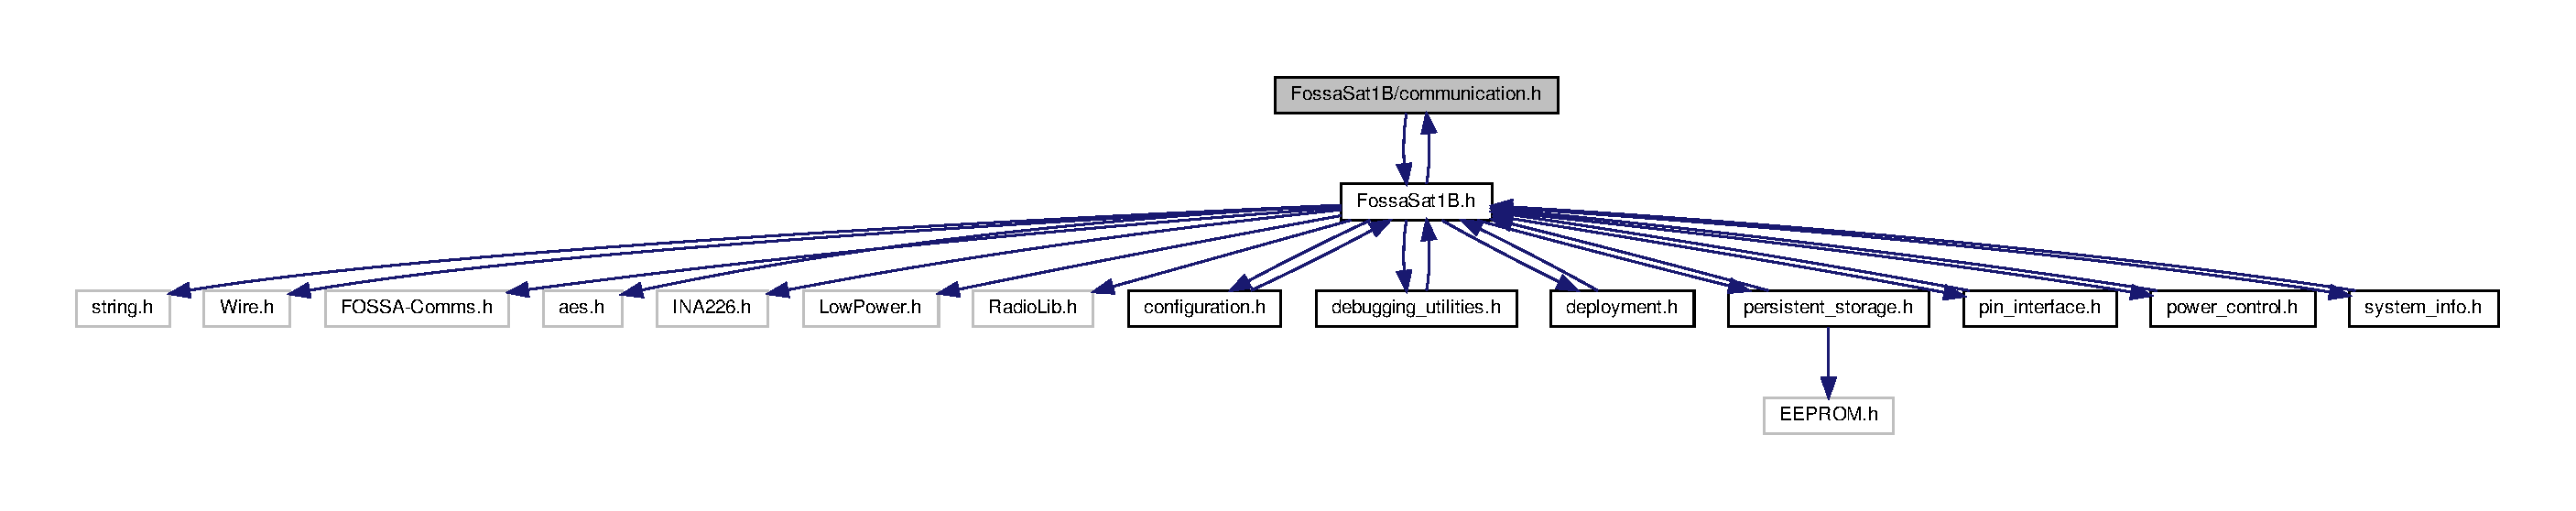
\includegraphics[width=350pt]{communication_8h__incl}
\end{center}
\end{figure}
This graph shows which files directly or indirectly include this file\+:
\nopagebreak
\begin{figure}[H]
\begin{center}
\leavevmode
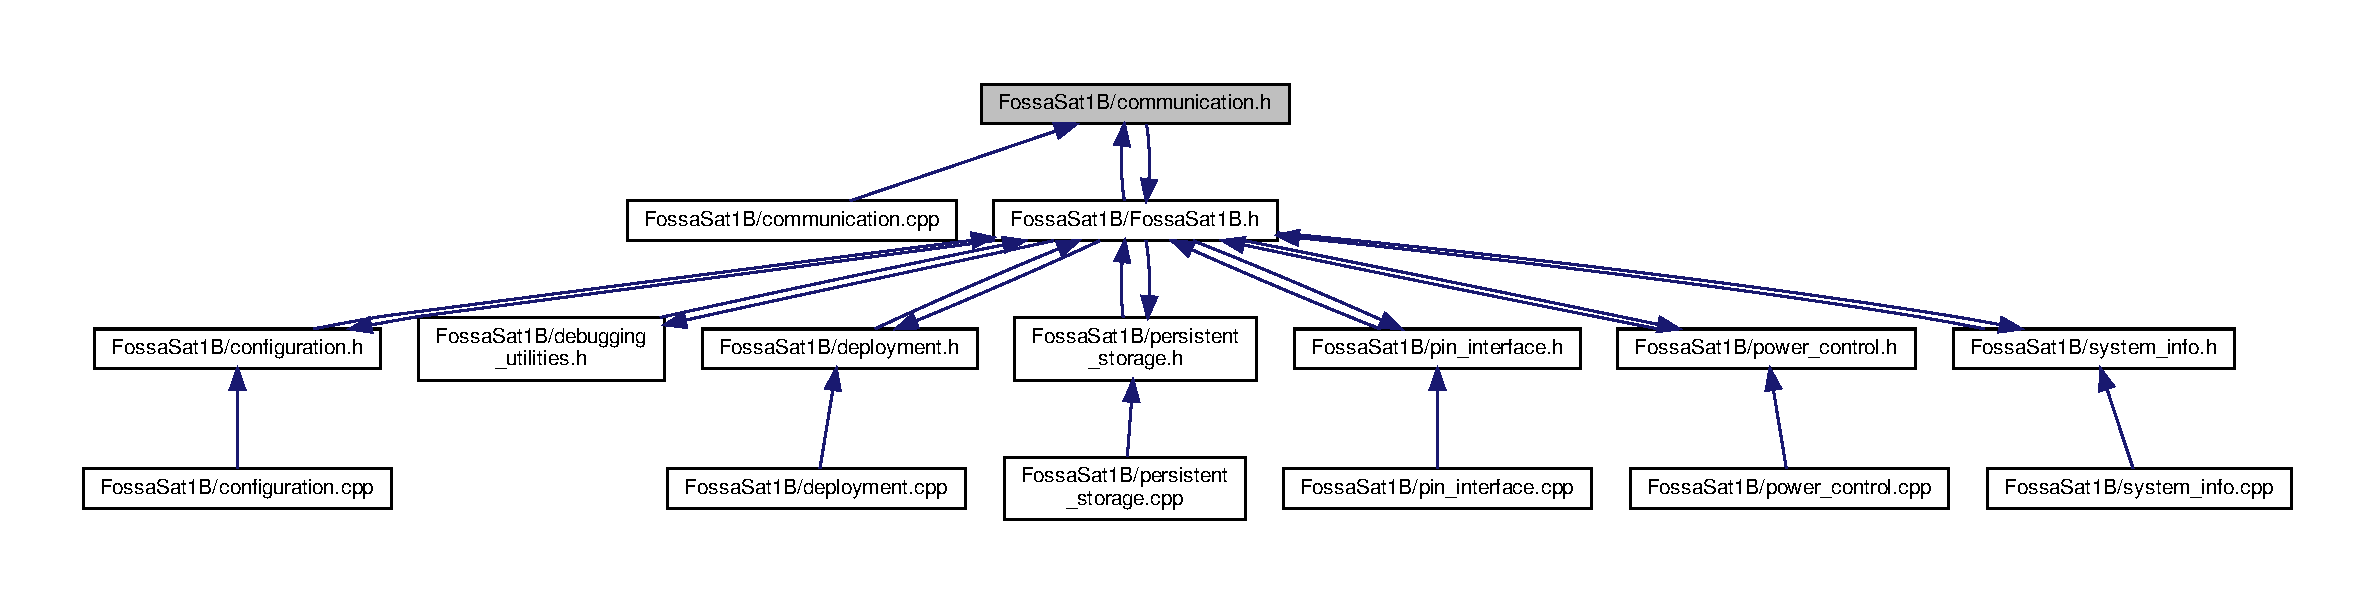
\includegraphics[width=350pt]{communication_8h__dep__incl}
\end{center}
\end{figure}
\subsection*{Functions}
\begin{DoxyCompactItemize}
\item 
void \hyperlink{communication_8h_aaadcd86dea525de318e35078c63b3149}{Communication\+\_\+\+Receive\+\_\+\+Interrupt} ()
\begin{DoxyCompactList}\small\item\em This function is called by the I\+SR when a transmission is received. \end{DoxyCompactList}\item 
int16\+\_\+t \hyperlink{communication_8h_a0183d47f45dfdb348647c3db1a75b73c}{Communication\+\_\+\+Set\+\_\+\+Modem} (uint8\+\_\+t modem)
\begin{DoxyCompactList}\small\item\em This function configures the radio to the given modem. \end{DoxyCompactList}\item 
int16\+\_\+t \hyperlink{communication_8h_a59478c57f2735f94bf2f19a272a75c02}{Communication\+\_\+\+Set\+\_\+\+Configuration} (uint8\+\_\+t $\ast$opt\+Data, uint8\+\_\+t opt\+Data\+Len)
\begin{DoxyCompactList}\small\item\em This function sets the configuration of the radio, which is used to Radio.\+Begin(). \end{DoxyCompactList}\item 
int16\+\_\+t \hyperlink{communication_8h_ad184c979eb82cc1c8d4fc32a802cb758}{Communication\+\_\+\+Set\+\_\+\+Spreading\+Factor} (uint8\+\_\+t sf\+Mode)
\begin{DoxyCompactList}\small\item\em This function sets the spreading factor of the radio. \end{DoxyCompactList}\item 
void \hyperlink{communication_8h_a5db7440be24bedc9c14f12db46029968}{Communication\+\_\+\+Send\+\_\+\+Morse\+\_\+\+Beacon} (float batt\+Voltage)
\begin{DoxyCompactList}\small\item\em This function transmits a morse beacon message. \end{DoxyCompactList}\item 
void \hyperlink{communication_8h_aee0a3df78da4459c808120a803c65b61}{Communication\+\_\+\+C\+W\+\_\+\+Beep} (uint32\+\_\+t len)
\begin{DoxyCompactList}\small\item\em This function transmits a continous wave \char`\"{}\+B\+E\+E\+P\char`\"{}". \end{DoxyCompactList}\item 
{\footnotesize template$<$typename T $>$ }\\void \hyperlink{communication_8h_a980dd25e42aaeac1620dc7f9b42859a2}{Communication\+\_\+\+Frame\+\_\+\+Add} (uint8\+\_\+t $\ast$$\ast$buff\+Ptr, T val, const char $\ast$name, uint32\+\_\+t mult, const char $\ast$unit)
\begin{DoxyCompactList}\small\item\em This function adds frame entry to a frame. \end{DoxyCompactList}\item 
void \hyperlink{communication_8h_ae4e350e62342431fda2184ff0dc47a65}{Communication\+\_\+\+Send\+\_\+\+System\+\_\+\+Info} ()
\begin{DoxyCompactList}\small\item\em Send the satellite\textquotesingle{}s information via the configured radio settings. \end{DoxyCompactList}\item 
void \hyperlink{communication_8h_a03f49b9aabc52b55893829b7069efc7b}{Communication\+\_\+\+Acknowledge} (uint8\+\_\+t function\+Id, uint8\+\_\+t result)
\begin{DoxyCompactList}\small\item\em This function sends acknowledge for a received frame. \end{DoxyCompactList}\item 
void \hyperlink{communication_8h_ad5052f7320724c62bfab348ea62c66ce}{Communication\+\_\+\+Process\+\_\+\+Packet} ()
\begin{DoxyCompactList}\small\item\em This function reads the contents of the radio when it receives a transmission. \end{DoxyCompactList}\item 
void \hyperlink{communication_8h_ab6495de804d5d54d071fe8b4dd408aba}{Comunication\+\_\+\+Parse\+\_\+\+Frame} (uint8\+\_\+t $\ast$frame, size\+\_\+t len)
\begin{DoxyCompactList}\small\item\em This function parses the internal contents of the message using the F\+O\+S\+SA C\+O\+M\+MS Protocol. \end{DoxyCompactList}\item 
void \hyperlink{communication_8h_a834526d017e482716c6061772d644d5b}{Communication\+\_\+\+Execute\+\_\+\+Function} (uint8\+\_\+t function\+Id, uint8\+\_\+t $\ast$opt\+Data=N\+U\+LL, size\+\_\+t opt\+Data\+Len=0)
\begin{DoxyCompactList}\small\item\em This function executes the given function id provided with the given data. \end{DoxyCompactList}\item 
int16\+\_\+t \hyperlink{communication_8h_af86331e2820ea70a7928919915937077}{Communication\+\_\+\+Send\+\_\+\+Response} (uint8\+\_\+t resp\+Id, uint8\+\_\+t $\ast$opt\+Data=nullptr, size\+\_\+t opt\+Data\+Len=0, bool override\+Modem=false)
\begin{DoxyCompactList}\small\item\em Responds to a given function id execution (internally used). \end{DoxyCompactList}\item 
int16\+\_\+t \hyperlink{communication_8h_a46802cdf83e9de4cab3ebd4a00256aeb}{Communication\+\_\+\+Transmit} (uint8\+\_\+t $\ast$data, uint8\+\_\+t len, bool override\+Modem=true)
\begin{DoxyCompactList}\small\item\em Transmits the given data. \end{DoxyCompactList}\item 
bool \hyperlink{communication_8h_abe2c8a0d33c8d6a33fe6fd33c729a5a9}{Communication\+\_\+\+Check\+\_\+\+Opt\+Data\+Len} (uint8\+\_\+t expected, uint8\+\_\+t actual)
\begin{DoxyCompactList}\small\item\em Helper functions to check two variables are equal, with debug prints. \end{DoxyCompactList}\end{DoxyCompactItemize}


\subsection{Detailed Description}
This system is the main interface that is used to transmit message, configure the radio and process received transmissions. 



\subsection{Function Documentation}
\mbox{\Hypertarget{communication_8h_a03f49b9aabc52b55893829b7069efc7b}\label{communication_8h_a03f49b9aabc52b55893829b7069efc7b}} 
\index{communication.\+h@{communication.\+h}!Communication\+\_\+\+Acknowledge@{Communication\+\_\+\+Acknowledge}}
\index{Communication\+\_\+\+Acknowledge@{Communication\+\_\+\+Acknowledge}!communication.\+h@{communication.\+h}}
\subsubsection{\texorpdfstring{Communication\+\_\+\+Acknowledge()}{Communication\_Acknowledge()}}
{\footnotesize\ttfamily void Communication\+\_\+\+Acknowledge (\begin{DoxyParamCaption}\item[{uint8\+\_\+t}]{function\+Id,  }\item[{uint8\+\_\+t}]{result }\end{DoxyParamCaption})}



This function sends acknowledge for a received frame. 

\begin{DoxyRefDesc}{Test}
\item[\hyperlink{test__test000009}{Test}](ID C\+O\+M\+M\+S\+\_\+\+H\+\_\+\+T10) (S\+EV 1) Test that each command/packet is processed correctly.\end{DoxyRefDesc}



\begin{DoxyParams}{Parameters}
{\em function\+Id} & Function ID to acknowledge. \\
\hline
{\em result} & Result of frame processing. \\
\hline
\end{DoxyParams}


Definition at line 238 of file communication.\+cpp.

Here is the call graph for this function\+:
\nopagebreak
\begin{figure}[H]
\begin{center}
\leavevmode
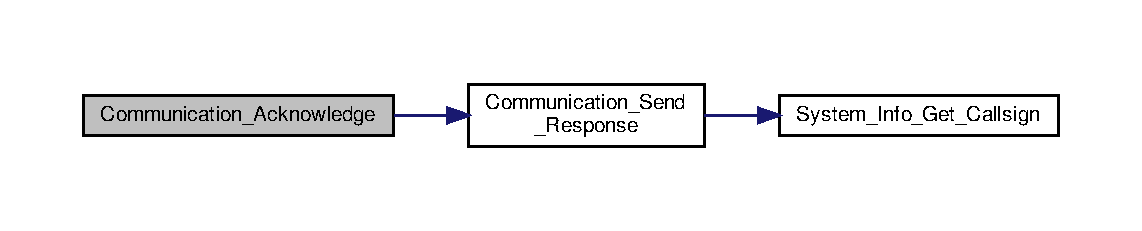
\includegraphics[width=350pt]{communication_8h_a03f49b9aabc52b55893829b7069efc7b_cgraph}
\end{center}
\end{figure}
Here is the caller graph for this function\+:
\nopagebreak
\begin{figure}[H]
\begin{center}
\leavevmode
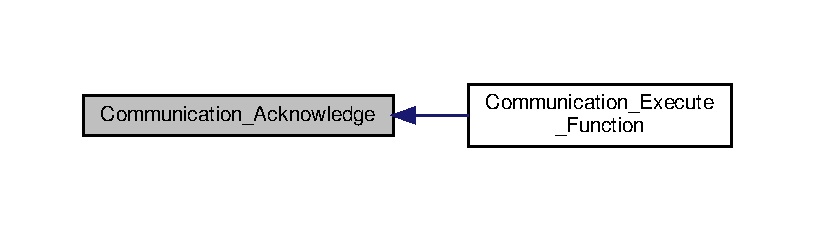
\includegraphics[width=350pt]{communication_8h_a03f49b9aabc52b55893829b7069efc7b_icgraph}
\end{center}
\end{figure}
\mbox{\Hypertarget{communication_8h_abe2c8a0d33c8d6a33fe6fd33c729a5a9}\label{communication_8h_abe2c8a0d33c8d6a33fe6fd33c729a5a9}} 
\index{communication.\+h@{communication.\+h}!Communication\+\_\+\+Check\+\_\+\+Opt\+Data\+Len@{Communication\+\_\+\+Check\+\_\+\+Opt\+Data\+Len}}
\index{Communication\+\_\+\+Check\+\_\+\+Opt\+Data\+Len@{Communication\+\_\+\+Check\+\_\+\+Opt\+Data\+Len}!communication.\+h@{communication.\+h}}
\subsubsection{\texorpdfstring{Communication\+\_\+\+Check\+\_\+\+Opt\+Data\+Len()}{Communication\_Check\_OptDataLen()}}
{\footnotesize\ttfamily bool Communication\+\_\+\+Check\+\_\+\+Opt\+Data\+Len (\begin{DoxyParamCaption}\item[{uint8\+\_\+t}]{expected,  }\item[{uint8\+\_\+t}]{actual }\end{DoxyParamCaption})}



Helper functions to check two variables are equal, with debug prints. 

\begin{DoxyRefDesc}{Test}
\item[\hyperlink{test__test000015}{Test}](ID C\+O\+M\+M\+S\+\_\+\+H\+\_\+\+T14) (S\+EV 1) Check that this function equates correctly.\end{DoxyRefDesc}



\begin{DoxyParams}{Parameters}
{\em expected} & The expected value \\
\hline
{\em actual} & The given value. \\
\hline
\end{DoxyParams}
\begin{DoxyReturn}{Returns}
true They are the same value. 

false They are not the same value. 
\end{DoxyReturn}


Definition at line 798 of file communication.\+cpp.

\mbox{\Hypertarget{communication_8h_aee0a3df78da4459c808120a803c65b61}\label{communication_8h_aee0a3df78da4459c808120a803c65b61}} 
\index{communication.\+h@{communication.\+h}!Communication\+\_\+\+C\+W\+\_\+\+Beep@{Communication\+\_\+\+C\+W\+\_\+\+Beep}}
\index{Communication\+\_\+\+C\+W\+\_\+\+Beep@{Communication\+\_\+\+C\+W\+\_\+\+Beep}!communication.\+h@{communication.\+h}}
\subsubsection{\texorpdfstring{Communication\+\_\+\+C\+W\+\_\+\+Beep()}{Communication\_CW\_Beep()}}
{\footnotesize\ttfamily void Communication\+\_\+\+C\+W\+\_\+\+Beep (\begin{DoxyParamCaption}\item[{uint32\+\_\+t}]{len }\end{DoxyParamCaption})}



This function transmits a continous wave \char`\"{}\+B\+E\+E\+P\char`\"{}". 

\begin{DoxyRefDesc}{Test}
\item[\hyperlink{test__test000006}{Test}](ID C\+O\+M\+M\+S\+\_\+\+H\+\_\+\+T7) (S\+EV 2) Test that the CW beep is received ok.\end{DoxyRefDesc}



\begin{DoxyParams}{Parameters}
{\em len} & Length of the beep in ms, with 500 ms resolution \\
\hline
\end{DoxyParams}


Definition at line 154 of file communication.\+cpp.

Here is the call graph for this function\+:
\nopagebreak
\begin{figure}[H]
\begin{center}
\leavevmode
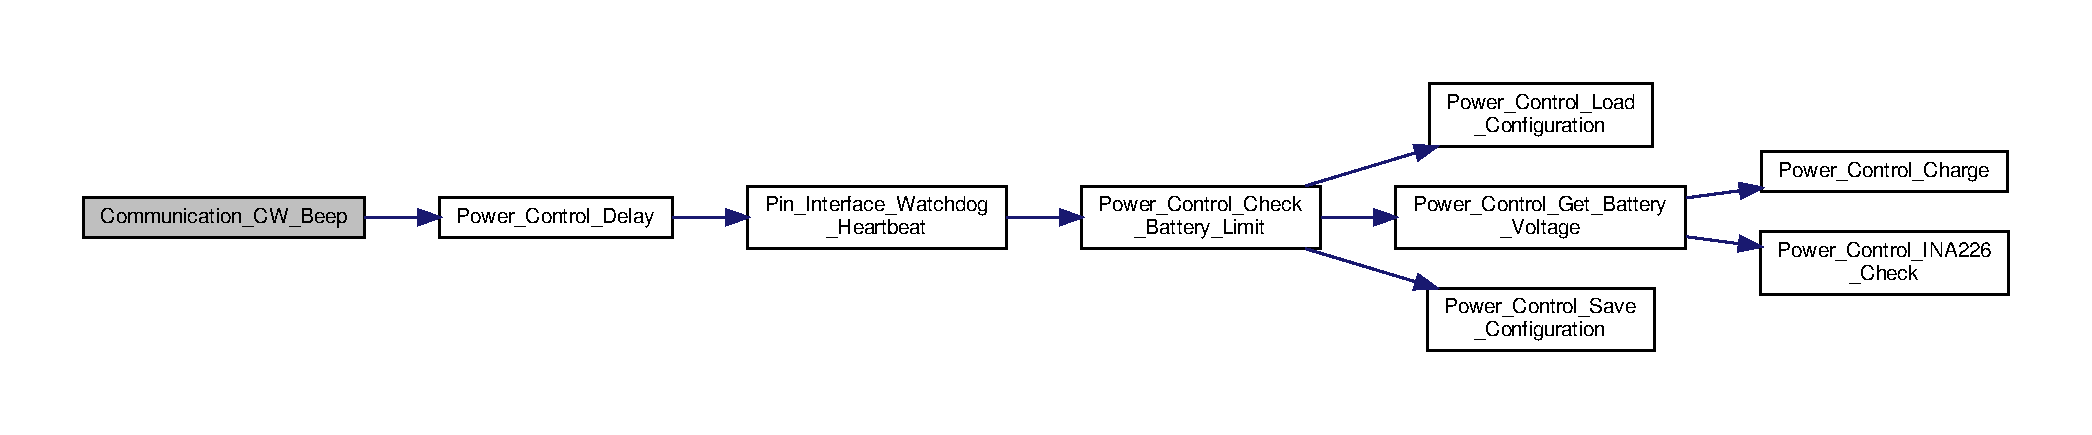
\includegraphics[width=350pt]{communication_8h_aee0a3df78da4459c808120a803c65b61_cgraph}
\end{center}
\end{figure}
\mbox{\Hypertarget{communication_8h_a834526d017e482716c6061772d644d5b}\label{communication_8h_a834526d017e482716c6061772d644d5b}} 
\index{communication.\+h@{communication.\+h}!Communication\+\_\+\+Execute\+\_\+\+Function@{Communication\+\_\+\+Execute\+\_\+\+Function}}
\index{Communication\+\_\+\+Execute\+\_\+\+Function@{Communication\+\_\+\+Execute\+\_\+\+Function}!communication.\+h@{communication.\+h}}
\subsubsection{\texorpdfstring{Communication\+\_\+\+Execute\+\_\+\+Function()}{Communication\_Execute\_Function()}}
{\footnotesize\ttfamily void Communication\+\_\+\+Execute\+\_\+\+Function (\begin{DoxyParamCaption}\item[{uint8\+\_\+t}]{function\+Id,  }\item[{uint8\+\_\+t $\ast$}]{opt\+Data = {\ttfamily NULL},  }\item[{size\+\_\+t}]{opt\+Data\+Len = {\ttfamily 0} }\end{DoxyParamCaption})}



This function executes the given function id provided with the given data. 

\begin{DoxyRefDesc}{Test}
\item[\hyperlink{test__test000012}{Test}](ID C\+O\+M\+M\+S\+\_\+\+H\+\_\+\+T11) (S\+EV 1) Test that each command is responded to with the correct function and data.\end{DoxyRefDesc}



\begin{DoxyParams}{Parameters}
{\em function\+Id} & The function to execute. \\
\hline
{\em opt\+Data} & The data to give to the function. \\
\hline
{\em opt\+Data\+Len} & The length of the data that is given to the function. \\
\hline
\end{DoxyParams}


Definition at line 375 of file communication.\+cpp.

Here is the call graph for this function\+:
\nopagebreak
\begin{figure}[H]
\begin{center}
\leavevmode
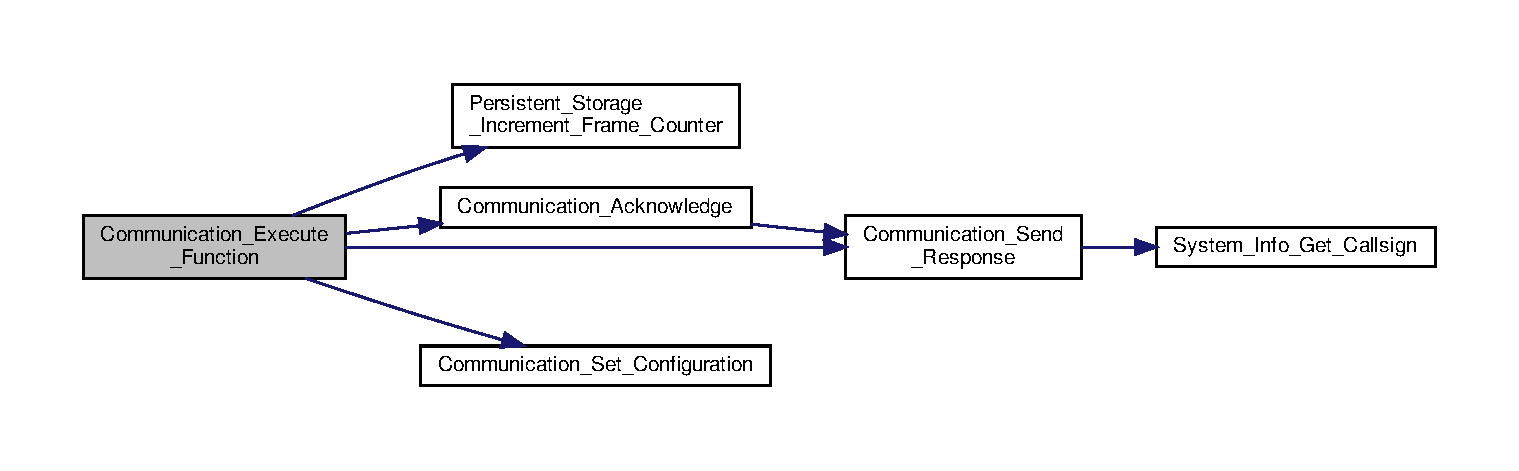
\includegraphics[width=350pt]{communication_8h_a834526d017e482716c6061772d644d5b_cgraph}
\end{center}
\end{figure}
\mbox{\Hypertarget{communication_8h_a980dd25e42aaeac1620dc7f9b42859a2}\label{communication_8h_a980dd25e42aaeac1620dc7f9b42859a2}} 
\index{communication.\+h@{communication.\+h}!Communication\+\_\+\+Frame\+\_\+\+Add@{Communication\+\_\+\+Frame\+\_\+\+Add}}
\index{Communication\+\_\+\+Frame\+\_\+\+Add@{Communication\+\_\+\+Frame\+\_\+\+Add}!communication.\+h@{communication.\+h}}
\subsubsection{\texorpdfstring{Communication\+\_\+\+Frame\+\_\+\+Add()}{Communication\_Frame\_Add()}}
{\footnotesize\ttfamily template$<$typename T $>$ \\
void Communication\+\_\+\+Frame\+\_\+\+Add (\begin{DoxyParamCaption}\item[{uint8\+\_\+t $\ast$$\ast$}]{buff\+Ptr,  }\item[{T}]{val,  }\item[{const char $\ast$}]{name,  }\item[{uint32\+\_\+t}]{mult,  }\item[{const char $\ast$}]{unit }\end{DoxyParamCaption})}



This function adds frame entry to a frame. 

\begin{DoxyRefDesc}{Test}
\item[\hyperlink{test__test000007}{Test}](ID C\+O\+M\+M\+S\+\_\+\+H\+\_\+\+T8) (S\+EV 1) Test that the system information is received correctly.\end{DoxyRefDesc}



\begin{DoxyParams}{Parameters}
{\em buff\+Ptr} & Pointer to the frame buffer. \\
\hline
{\em val} & Value to be added. \\
\hline
{\em name} & Name of the parameter (debug only); \\
\hline
{\em mult} & Multiplier of the parameter (debug only); \\
\hline
{\em unit} & Unit of the parameter (debug only); \\
\hline
\end{DoxyParams}


Definition at line 83 of file communication.\+h.

Here is the caller graph for this function\+:
\nopagebreak
\begin{figure}[H]
\begin{center}
\leavevmode
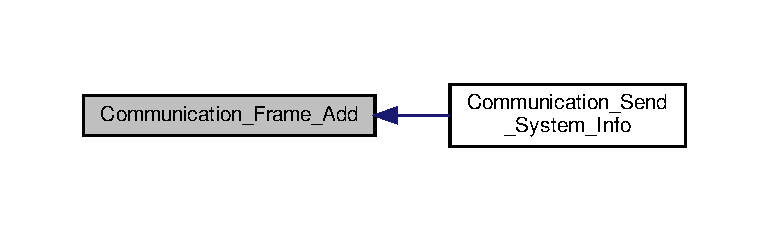
\includegraphics[width=350pt]{communication_8h_a980dd25e42aaeac1620dc7f9b42859a2_icgraph}
\end{center}
\end{figure}
\mbox{\Hypertarget{communication_8h_ad5052f7320724c62bfab348ea62c66ce}\label{communication_8h_ad5052f7320724c62bfab348ea62c66ce}} 
\index{communication.\+h@{communication.\+h}!Communication\+\_\+\+Process\+\_\+\+Packet@{Communication\+\_\+\+Process\+\_\+\+Packet}}
\index{Communication\+\_\+\+Process\+\_\+\+Packet@{Communication\+\_\+\+Process\+\_\+\+Packet}!communication.\+h@{communication.\+h}}
\subsubsection{\texorpdfstring{Communication\+\_\+\+Process\+\_\+\+Packet()}{Communication\_Process\_Packet()}}
{\footnotesize\ttfamily void Communication\+\_\+\+Process\+\_\+\+Packet (\begin{DoxyParamCaption}{ }\end{DoxyParamCaption})}



This function reads the contents of the radio when it receives a transmission. 

\begin{DoxyRefDesc}{Test}
\item[\hyperlink{test__test000010}{Test}](ID C\+O\+M\+M\+S\+\_\+\+H\+\_\+\+T9) (S\+EV 1) Test that each command/packet is processed correctly.\end{DoxyRefDesc}


Definition at line 243 of file communication.\+cpp.

\mbox{\Hypertarget{communication_8h_aaadcd86dea525de318e35078c63b3149}\label{communication_8h_aaadcd86dea525de318e35078c63b3149}} 
\index{communication.\+h@{communication.\+h}!Communication\+\_\+\+Receive\+\_\+\+Interrupt@{Communication\+\_\+\+Receive\+\_\+\+Interrupt}}
\index{Communication\+\_\+\+Receive\+\_\+\+Interrupt@{Communication\+\_\+\+Receive\+\_\+\+Interrupt}!communication.\+h@{communication.\+h}}
\subsubsection{\texorpdfstring{Communication\+\_\+\+Receive\+\_\+\+Interrupt()}{Communication\_Receive\_Interrupt()}}
{\footnotesize\ttfamily void Communication\+\_\+\+Receive\+\_\+\+Interrupt (\begin{DoxyParamCaption}{ }\end{DoxyParamCaption})}



This function is called by the I\+SR when a transmission is received. 

\begin{DoxyRefDesc}{Test}
\item[\hyperlink{test__test000001}{Test}](ID C\+O\+M\+M\+S\+\_\+\+H\+\_\+\+T0) (S\+EV 1) Make sure this function is called when the radio receives data.\end{DoxyRefDesc}


Definition at line 3 of file communication.\+cpp.

\mbox{\Hypertarget{communication_8h_a5db7440be24bedc9c14f12db46029968}\label{communication_8h_a5db7440be24bedc9c14f12db46029968}} 
\index{communication.\+h@{communication.\+h}!Communication\+\_\+\+Send\+\_\+\+Morse\+\_\+\+Beacon@{Communication\+\_\+\+Send\+\_\+\+Morse\+\_\+\+Beacon}}
\index{Communication\+\_\+\+Send\+\_\+\+Morse\+\_\+\+Beacon@{Communication\+\_\+\+Send\+\_\+\+Morse\+\_\+\+Beacon}!communication.\+h@{communication.\+h}}
\subsubsection{\texorpdfstring{Communication\+\_\+\+Send\+\_\+\+Morse\+\_\+\+Beacon()}{Communication\_Send\_Morse\_Beacon()}}
{\footnotesize\ttfamily void Communication\+\_\+\+Send\+\_\+\+Morse\+\_\+\+Beacon (\begin{DoxyParamCaption}\item[{float}]{batt\+Voltage }\end{DoxyParamCaption})}



This function transmits a morse beacon message. 

\begin{DoxyRefDesc}{Test}
\item[\hyperlink{test__test000005}{Test}](ID C\+O\+M\+M\+S\+\_\+\+H\+\_\+\+T5) (S\+EV 1) Test that the beacon message can be received properly. 

(ID C\+O\+M\+M\+S\+\_\+\+H\+\_\+\+T6) (S\+EV 1) Test that the beacon messages battery voltage is received ok.\end{DoxyRefDesc}



\begin{DoxyParams}{Parameters}
{\em batt\+Voltage} & The battery voltage to send via morse code. \\
\hline
\end{DoxyParams}


Definition at line 123 of file communication.\+cpp.

Here is the call graph for this function\+:
\nopagebreak
\begin{figure}[H]
\begin{center}
\leavevmode
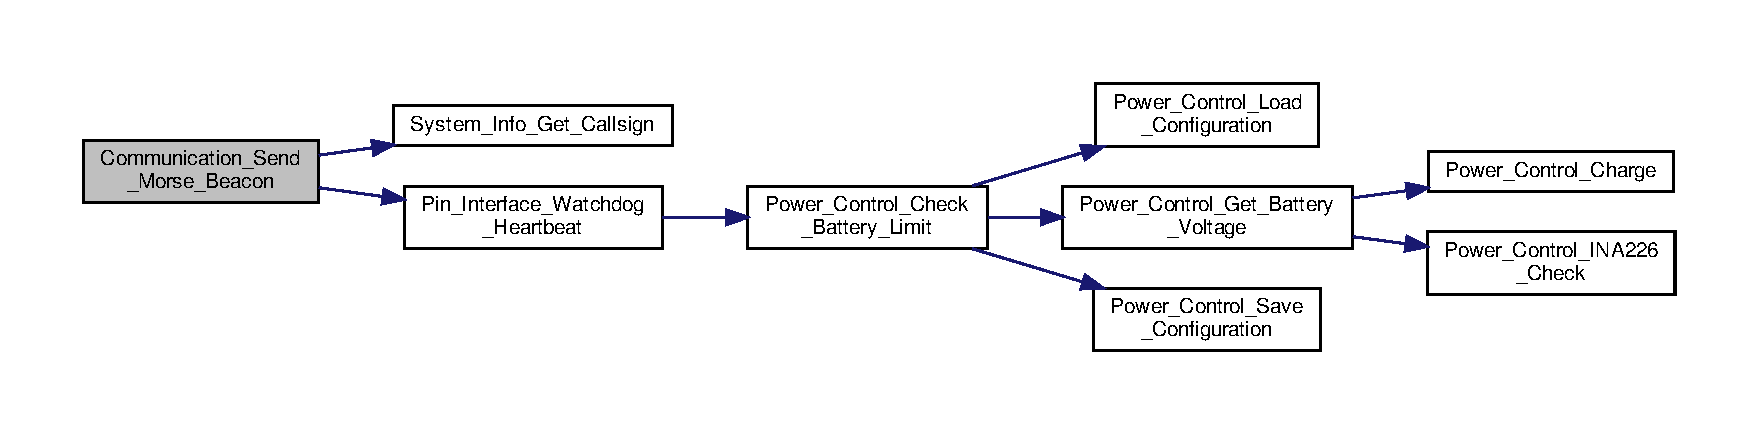
\includegraphics[width=350pt]{communication_8h_a5db7440be24bedc9c14f12db46029968_cgraph}
\end{center}
\end{figure}
\mbox{\Hypertarget{communication_8h_af86331e2820ea70a7928919915937077}\label{communication_8h_af86331e2820ea70a7928919915937077}} 
\index{communication.\+h@{communication.\+h}!Communication\+\_\+\+Send\+\_\+\+Response@{Communication\+\_\+\+Send\+\_\+\+Response}}
\index{Communication\+\_\+\+Send\+\_\+\+Response@{Communication\+\_\+\+Send\+\_\+\+Response}!communication.\+h@{communication.\+h}}
\subsubsection{\texorpdfstring{Communication\+\_\+\+Send\+\_\+\+Response()}{Communication\_Send\_Response()}}
{\footnotesize\ttfamily int16\+\_\+t Communication\+\_\+\+Send\+\_\+\+Response (\begin{DoxyParamCaption}\item[{uint8\+\_\+t}]{resp\+Id,  }\item[{uint8\+\_\+t $\ast$}]{opt\+Data = {\ttfamily nullptr},  }\item[{size\+\_\+t}]{opt\+Data\+Len = {\ttfamily 0},  }\item[{bool}]{override\+Modem = {\ttfamily false} }\end{DoxyParamCaption})}



Responds to a given function id execution (internally used). 

\begin{DoxyRefDesc}{Test}
\item[\hyperlink{test__test000013}{Test}](ID C\+O\+M\+M\+S\+\_\+\+H\+\_\+\+T12) (S\+EV 1) Test that each response transmits correctly.\end{DoxyRefDesc}



\begin{DoxyParams}{Parameters}
{\em resp\+Id} & Function ID to respond with. \\
\hline
{\em opt\+Data} & The data to respond with. \\
\hline
{\em opt\+Data\+Len} & The length of the data to respond with. \\
\hline
{\em override\+Modem} & Override the modem to use default Lo\+Ra modem and settings. \\
\hline
\end{DoxyParams}
\begin{DoxyReturn}{Returns}
int16\+\_\+t The status code of the \hyperlink{communication_8h_a46802cdf83e9de4cab3ebd4a00256aeb}{Communication\+\_\+\+Transmit()} function. 
\end{DoxyReturn}


Definition at line 684 of file communication.\+cpp.

Here is the call graph for this function\+:
\nopagebreak
\begin{figure}[H]
\begin{center}
\leavevmode
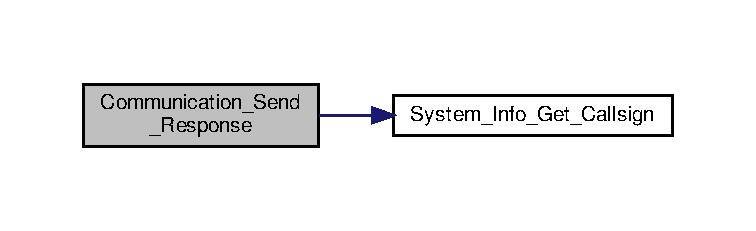
\includegraphics[width=350pt]{communication_8h_af86331e2820ea70a7928919915937077_cgraph}
\end{center}
\end{figure}
Here is the caller graph for this function\+:
\nopagebreak
\begin{figure}[H]
\begin{center}
\leavevmode
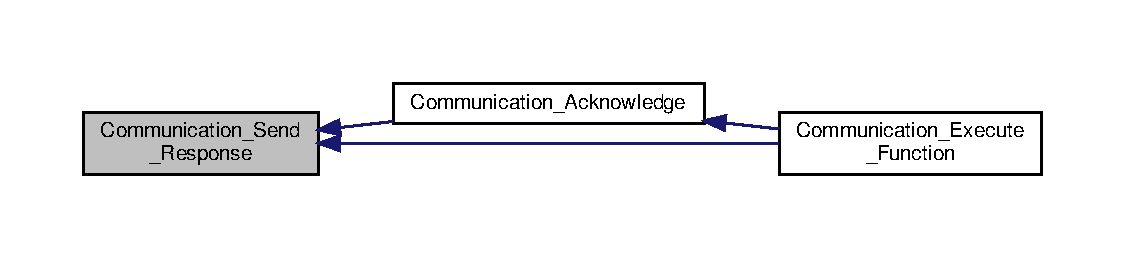
\includegraphics[width=350pt]{communication_8h_af86331e2820ea70a7928919915937077_icgraph}
\end{center}
\end{figure}
\mbox{\Hypertarget{communication_8h_ae4e350e62342431fda2184ff0dc47a65}\label{communication_8h_ae4e350e62342431fda2184ff0dc47a65}} 
\index{communication.\+h@{communication.\+h}!Communication\+\_\+\+Send\+\_\+\+System\+\_\+\+Info@{Communication\+\_\+\+Send\+\_\+\+System\+\_\+\+Info}}
\index{Communication\+\_\+\+Send\+\_\+\+System\+\_\+\+Info@{Communication\+\_\+\+Send\+\_\+\+System\+\_\+\+Info}!communication.\+h@{communication.\+h}}
\subsubsection{\texorpdfstring{Communication\+\_\+\+Send\+\_\+\+System\+\_\+\+Info()}{Communication\_Send\_System\_Info()}}
{\footnotesize\ttfamily void Communication\+\_\+\+Send\+\_\+\+System\+\_\+\+Info (\begin{DoxyParamCaption}{ }\end{DoxyParamCaption})}



Send the satellite\textquotesingle{}s information via the configured radio settings. 

\begin{DoxyRefDesc}{Test}
\item[\hyperlink{test__test000008}{Test}](ID C\+O\+M\+M\+S\+\_\+\+H\+\_\+\+T8) (S\+EV 1) Test that the system information is received correctly.\end{DoxyRefDesc}


Definition at line 160 of file communication.\+cpp.

Here is the call graph for this function\+:
\nopagebreak
\begin{figure}[H]
\begin{center}
\leavevmode
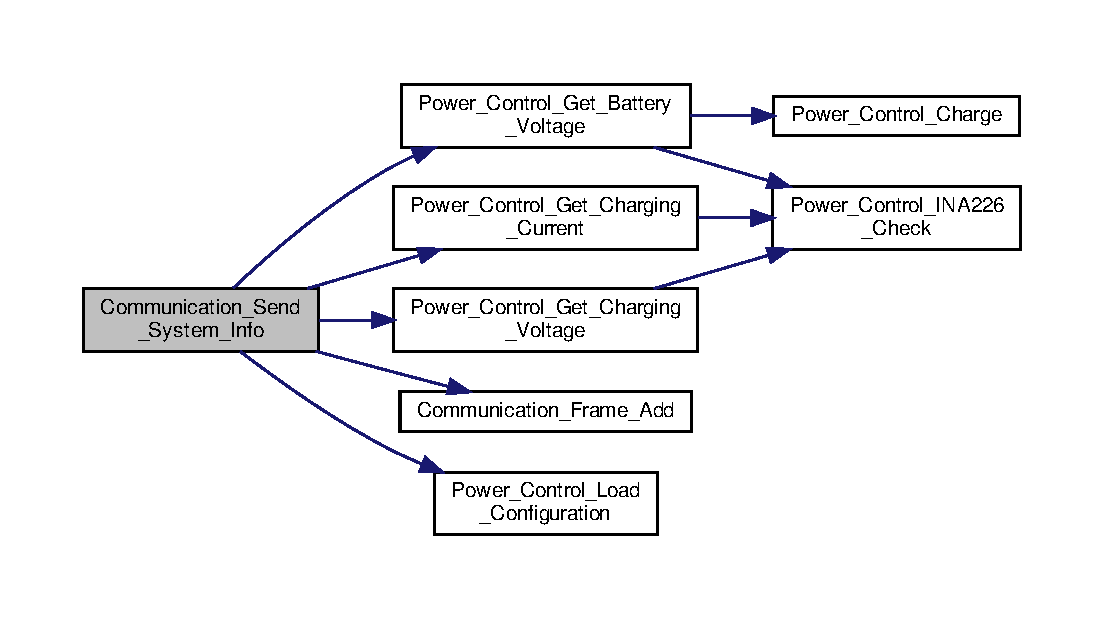
\includegraphics[width=350pt]{communication_8h_ae4e350e62342431fda2184ff0dc47a65_cgraph}
\end{center}
\end{figure}
\mbox{\Hypertarget{communication_8h_a59478c57f2735f94bf2f19a272a75c02}\label{communication_8h_a59478c57f2735f94bf2f19a272a75c02}} 
\index{communication.\+h@{communication.\+h}!Communication\+\_\+\+Set\+\_\+\+Configuration@{Communication\+\_\+\+Set\+\_\+\+Configuration}}
\index{Communication\+\_\+\+Set\+\_\+\+Configuration@{Communication\+\_\+\+Set\+\_\+\+Configuration}!communication.\+h@{communication.\+h}}
\subsubsection{\texorpdfstring{Communication\+\_\+\+Set\+\_\+\+Configuration()}{Communication\_Set\_Configuration()}}
{\footnotesize\ttfamily int16\+\_\+t Communication\+\_\+\+Set\+\_\+\+Configuration (\begin{DoxyParamCaption}\item[{uint8\+\_\+t $\ast$}]{opt\+Data,  }\item[{uint8\+\_\+t}]{opt\+Data\+Len }\end{DoxyParamCaption})}



This function sets the configuration of the radio, which is used to Radio.\+Begin(). 

\begin{DoxyRefDesc}{Test}
\item[\hyperlink{test__test000003}{Test}](ID C\+O\+M\+M\+S\+\_\+\+H\+\_\+\+T2) (S\+EV 1) Make sure the modem mode is changed with no errors.\end{DoxyRefDesc}



\begin{DoxyParams}{Parameters}
{\em opt\+Data} & The data which is used to configure the radio. \\
\hline
{\em opt\+Data\+Len} & The length of the byte string given. \\
\hline
\end{DoxyParams}
\begin{DoxyReturn}{Returns}
int16\+\_\+t The status code returned by the radio.\+Begin() function. 
\end{DoxyReturn}


Definition at line 91 of file communication.\+cpp.

Here is the caller graph for this function\+:
\nopagebreak
\begin{figure}[H]
\begin{center}
\leavevmode
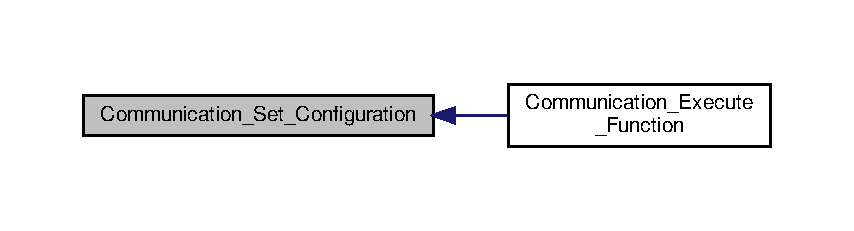
\includegraphics[width=350pt]{communication_8h_a59478c57f2735f94bf2f19a272a75c02_icgraph}
\end{center}
\end{figure}
\mbox{\Hypertarget{communication_8h_a0183d47f45dfdb348647c3db1a75b73c}\label{communication_8h_a0183d47f45dfdb348647c3db1a75b73c}} 
\index{communication.\+h@{communication.\+h}!Communication\+\_\+\+Set\+\_\+\+Modem@{Communication\+\_\+\+Set\+\_\+\+Modem}}
\index{Communication\+\_\+\+Set\+\_\+\+Modem@{Communication\+\_\+\+Set\+\_\+\+Modem}!communication.\+h@{communication.\+h}}
\subsubsection{\texorpdfstring{Communication\+\_\+\+Set\+\_\+\+Modem()}{Communication\_Set\_Modem()}}
{\footnotesize\ttfamily int16\+\_\+t Communication\+\_\+\+Set\+\_\+\+Modem (\begin{DoxyParamCaption}\item[{uint8\+\_\+t}]{modem }\end{DoxyParamCaption})}



This function configures the radio to the given modem. 

\begin{DoxyRefDesc}{Test}
\item[\hyperlink{test__test000002}{Test}](ID C\+O\+M\+M\+S\+\_\+\+H\+\_\+\+T1) (S\+EV 1) Make sure the modem mode is changed with no errors.\end{DoxyRefDesc}



\begin{DoxyParams}{Parameters}
{\em modem} & see \hyperlink{group__defines__radio__modem__configuration}{Modem Identifiers} \\
\hline
\end{DoxyParams}
\begin{DoxyReturn}{Returns}
int16\+\_\+t The Radio\+Lib status code for .Begin(). 
\end{DoxyReturn}


Definition at line 13 of file communication.\+cpp.

\mbox{\Hypertarget{communication_8h_ad184c979eb82cc1c8d4fc32a802cb758}\label{communication_8h_ad184c979eb82cc1c8d4fc32a802cb758}} 
\index{communication.\+h@{communication.\+h}!Communication\+\_\+\+Set\+\_\+\+Spreading\+Factor@{Communication\+\_\+\+Set\+\_\+\+Spreading\+Factor}}
\index{Communication\+\_\+\+Set\+\_\+\+Spreading\+Factor@{Communication\+\_\+\+Set\+\_\+\+Spreading\+Factor}!communication.\+h@{communication.\+h}}
\subsubsection{\texorpdfstring{Communication\+\_\+\+Set\+\_\+\+Spreading\+Factor()}{Communication\_Set\_SpreadingFactor()}}
{\footnotesize\ttfamily int16\+\_\+t Communication\+\_\+\+Set\+\_\+\+Spreading\+Factor (\begin{DoxyParamCaption}\item[{uint8\+\_\+t}]{sf\+Mode }\end{DoxyParamCaption})}



This function sets the spreading factor of the radio. 

\begin{DoxyRefDesc}{Test}
\item[\hyperlink{test__test000004}{Test}](ID C\+O\+M\+M\+S\+\_\+\+H\+\_\+\+T3) (S\+EV 1) Make sure the radio\textquotesingle{}s spreading factor can be changed with no errors. 

(ID C\+O\+M\+M\+S\+\_\+\+H\+\_\+\+T4) (S\+EV 1) Make sure the radio\textquotesingle{}s spreading factors are compatable with generic radios.\end{DoxyRefDesc}



\begin{DoxyParams}{Parameters}
{\em sf\+Mode} & See defines\+\_\+radio\+\_\+lora\+\_\+configuraiton \\
\hline
\end{DoxyParams}
\begin{DoxyReturn}{Returns}
int16\+\_\+t The status code returned by the radio.\+set\+Spreading\+Factor() function. 
\end{DoxyReturn}


Definition at line 72 of file communication.\+cpp.

\mbox{\Hypertarget{communication_8h_a46802cdf83e9de4cab3ebd4a00256aeb}\label{communication_8h_a46802cdf83e9de4cab3ebd4a00256aeb}} 
\index{communication.\+h@{communication.\+h}!Communication\+\_\+\+Transmit@{Communication\+\_\+\+Transmit}}
\index{Communication\+\_\+\+Transmit@{Communication\+\_\+\+Transmit}!communication.\+h@{communication.\+h}}
\subsubsection{\texorpdfstring{Communication\+\_\+\+Transmit()}{Communication\_Transmit()}}
{\footnotesize\ttfamily int16\+\_\+t Communication\+\_\+\+Transmit (\begin{DoxyParamCaption}\item[{uint8\+\_\+t $\ast$}]{data,  }\item[{uint8\+\_\+t}]{len,  }\item[{bool}]{override\+Modem = {\ttfamily true} }\end{DoxyParamCaption})}



Transmits the given data. 

\begin{DoxyRefDesc}{Test}
\item[\hyperlink{test__test000014}{Test}](ID C\+O\+M\+M\+S\+\_\+\+H\+\_\+\+T13) (S\+EV 1) Check that each function/command transmits correctly.\end{DoxyRefDesc}



\begin{DoxyParams}{Parameters}
{\em data} & The byte array to transmit. \\
\hline
{\em len} & The length of the byte array to transmit. \\
\hline
{\em override\+Modem} & Override the modem to use default Lo\+Ra modem and settings. \\
\hline
\end{DoxyParams}
\begin{DoxyReturn}{Returns}
int16\+\_\+t The status code of the Radio.\+Tranmit() function. 
\end{DoxyReturn}


Definition at line 705 of file communication.\+cpp.

Here is the call graph for this function\+:
\nopagebreak
\begin{figure}[H]
\begin{center}
\leavevmode
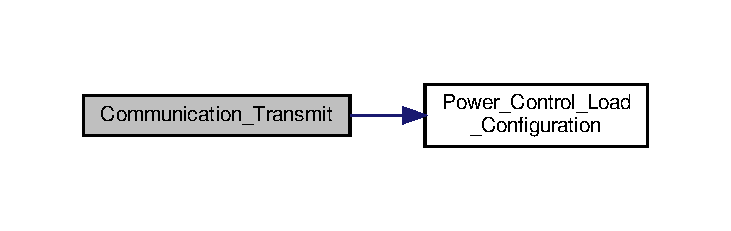
\includegraphics[width=350pt]{communication_8h_a46802cdf83e9de4cab3ebd4a00256aeb_cgraph}
\end{center}
\end{figure}
\mbox{\Hypertarget{communication_8h_ab6495de804d5d54d071fe8b4dd408aba}\label{communication_8h_ab6495de804d5d54d071fe8b4dd408aba}} 
\index{communication.\+h@{communication.\+h}!Comunication\+\_\+\+Parse\+\_\+\+Frame@{Comunication\+\_\+\+Parse\+\_\+\+Frame}}
\index{Comunication\+\_\+\+Parse\+\_\+\+Frame@{Comunication\+\_\+\+Parse\+\_\+\+Frame}!communication.\+h@{communication.\+h}}
\subsubsection{\texorpdfstring{Comunication\+\_\+\+Parse\+\_\+\+Frame()}{Comunication\_Parse\_Frame()}}
{\footnotesize\ttfamily void Comunication\+\_\+\+Parse\+\_\+\+Frame (\begin{DoxyParamCaption}\item[{uint8\+\_\+t $\ast$}]{frame,  }\item[{size\+\_\+t}]{len }\end{DoxyParamCaption})}



This function parses the internal contents of the message using the F\+O\+S\+SA C\+O\+M\+MS Protocol. 

\begin{DoxyRefDesc}{Test}
\item[\hyperlink{test__test000011}{Test}](ID C\+O\+M\+M\+S\+\_\+\+H\+\_\+\+T10) (S\+EV 1) Test that each command/packet is processed correctly.\end{DoxyRefDesc}



\begin{DoxyParams}{Parameters}
{\em frame} & The raw data to process. \\
\hline
{\em len} & The length of the raw data. \\
\hline
\end{DoxyParams}


Definition at line 290 of file communication.\+cpp.

Here is the call graph for this function\+:
\nopagebreak
\begin{figure}[H]
\begin{center}
\leavevmode
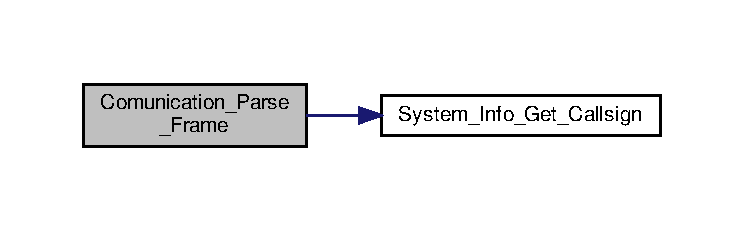
\includegraphics[width=350pt]{communication_8h_ab6495de804d5d54d071fe8b4dd408aba_cgraph}
\end{center}
\end{figure}

\hypertarget{debugging__utilities_8h}{}\section{Fossa\+Sat1\+B/debugging\+\_\+utilities.h File Reference}
\label{debugging__utilities_8h}\index{Fossa\+Sat1\+B/debugging\+\_\+utilities.\+h@{Fossa\+Sat1\+B/debugging\+\_\+utilities.\+h}}
{\ttfamily \#include \char`\"{}Fossa\+Sat1\+B.\+h\char`\"{}}\newline
Include dependency graph for debugging\+\_\+utilities.\+h\+:
\nopagebreak
\begin{figure}[H]
\begin{center}
\leavevmode
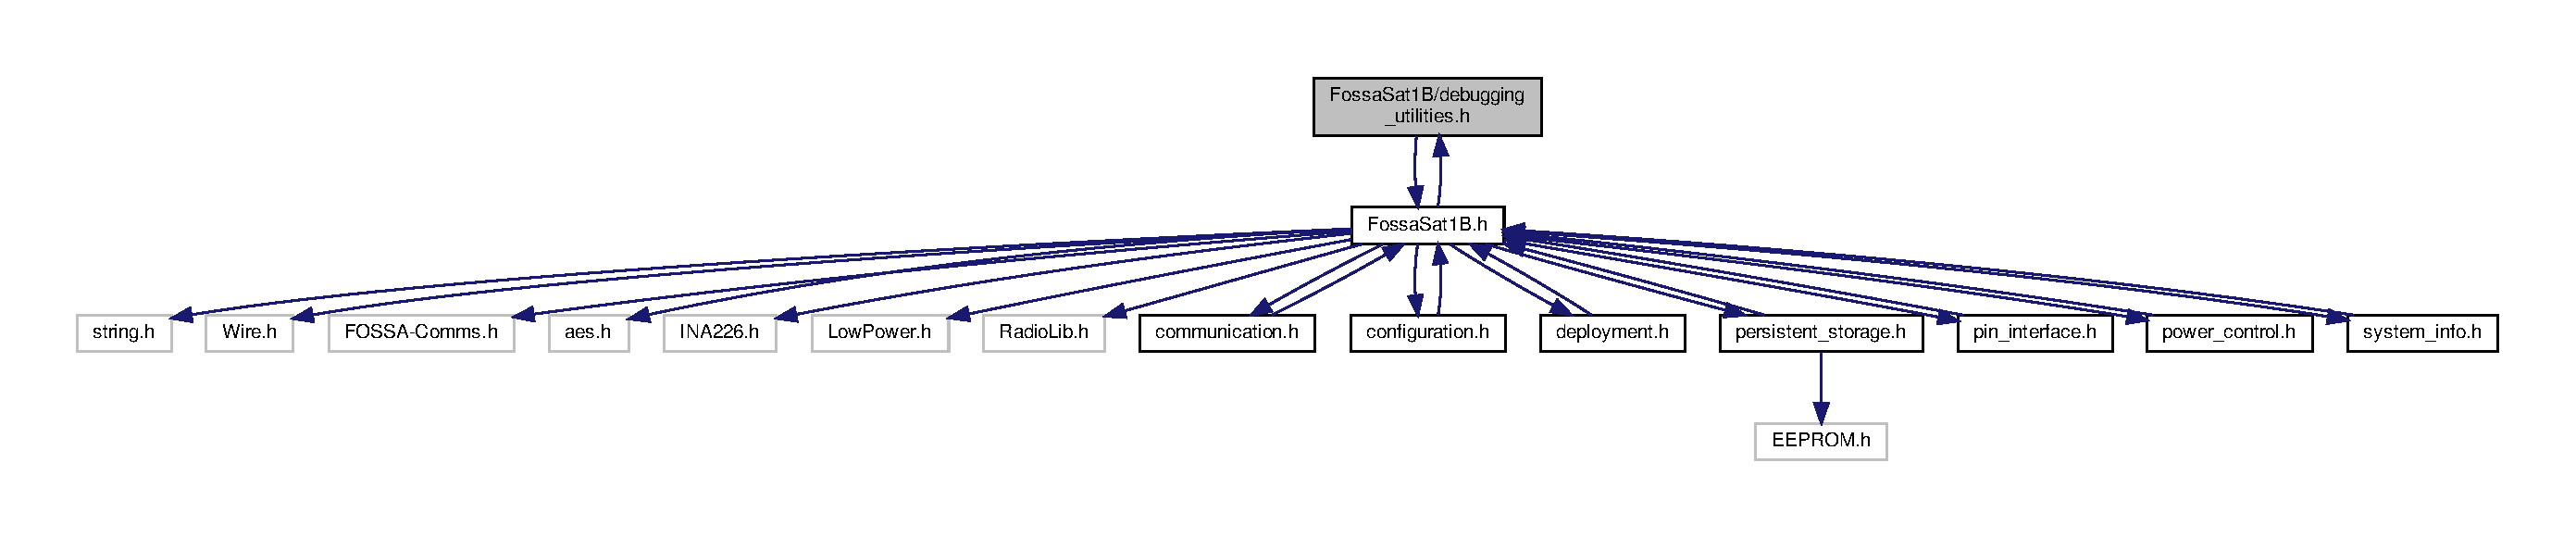
\includegraphics[width=350pt]{debugging__utilities_8h__incl}
\end{center}
\end{figure}
This graph shows which files directly or indirectly include this file\+:
\nopagebreak
\begin{figure}[H]
\begin{center}
\leavevmode
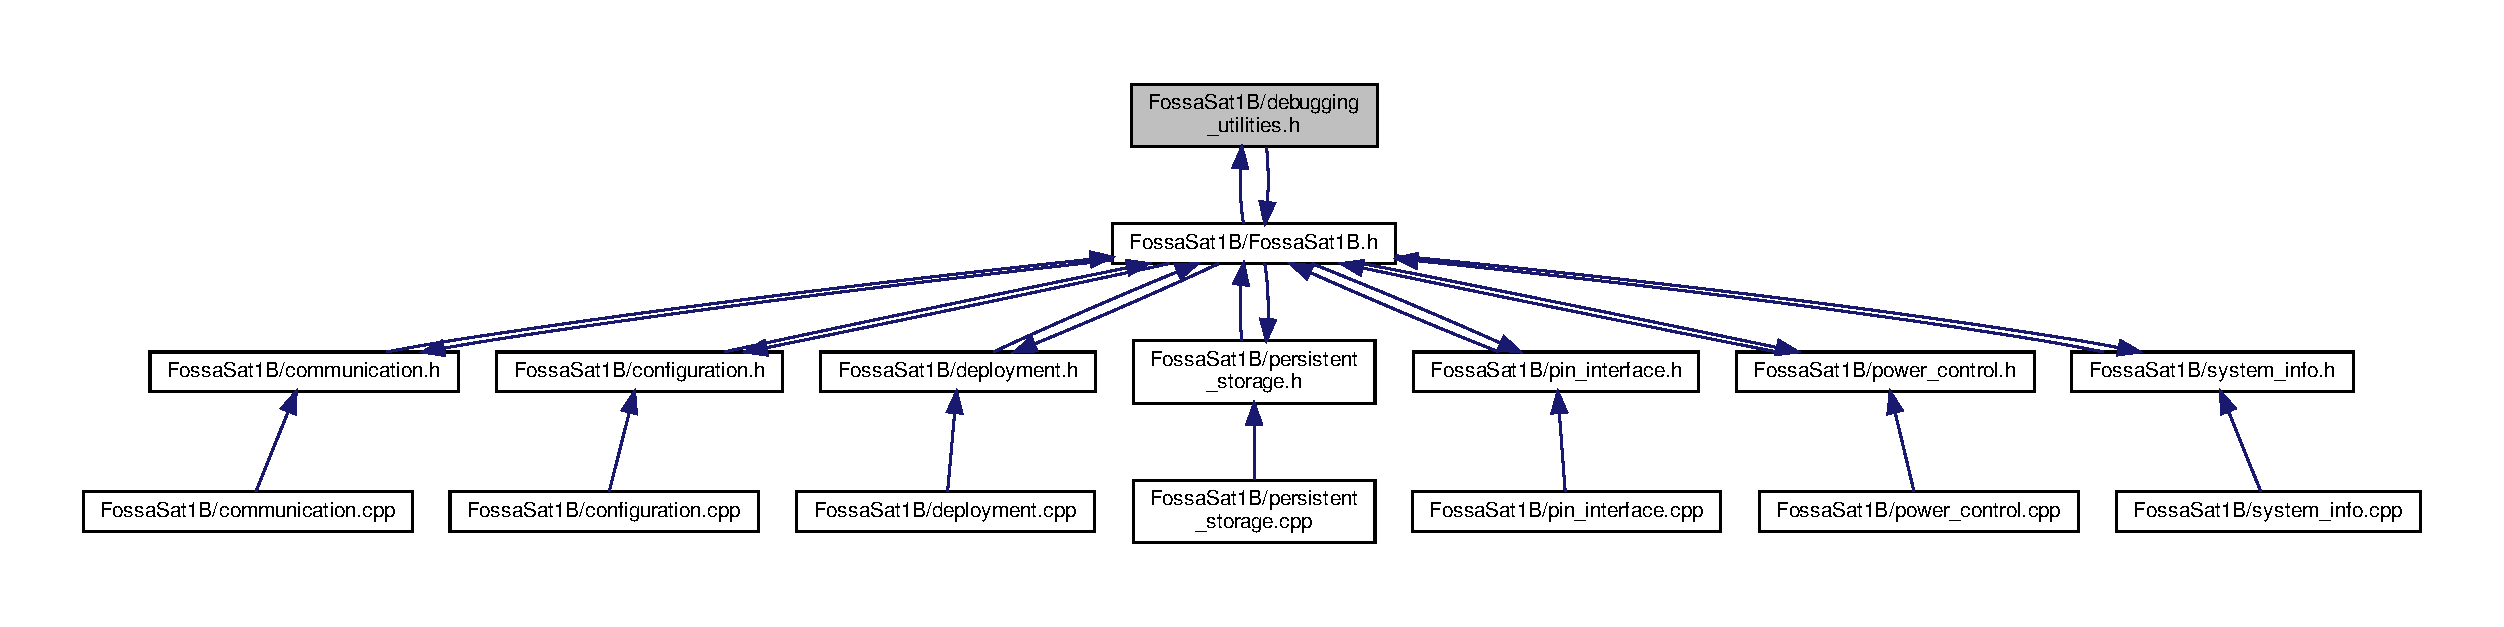
\includegraphics[width=350pt]{debugging__utilities_8h__dep__incl}
\end{center}
\end{figure}
\subsection*{Macros}
\begin{DoxyCompactItemize}
\item 
\#define {\bfseries F\+O\+S\+S\+A\+S\+A\+T\+\_\+\+D\+E\+B\+UG}
\item 
\#define {\bfseries F\+O\+S\+S\+A\+S\+A\+T\+\_\+\+D\+E\+B\+U\+G\+\_\+\+P\+O\+RT}~Serial
\item 
\#define {\bfseries F\+O\+S\+S\+A\+S\+A\+T\+\_\+\+D\+E\+B\+U\+G\+\_\+\+S\+P\+E\+ED}~115200
\item 
\#define {\bfseries F\+O\+S\+S\+A\+S\+A\+T\+\_\+\+D\+E\+B\+U\+G\+\_\+\+B\+E\+G\+IN}(...)~\{ F\+O\+S\+S\+A\+S\+A\+T\+\_\+\+D\+E\+B\+U\+G\+\_\+\+P\+O\+R\+T.\+begin(\+\_\+\+\_\+\+V\+A\+\_\+\+A\+R\+G\+S\+\_\+\+\_\+); \}
\item 
\#define {\bfseries F\+O\+S\+S\+A\+S\+A\+T\+\_\+\+D\+E\+B\+U\+G\+\_\+\+P\+R\+I\+NT}(...)~\{ F\+O\+S\+S\+A\+S\+A\+T\+\_\+\+D\+E\+B\+U\+G\+\_\+\+P\+O\+R\+T.\+print(\+\_\+\+\_\+\+V\+A\+\_\+\+A\+R\+G\+S\+\_\+\+\_\+); \}
\item 
\#define {\bfseries F\+O\+S\+S\+A\+S\+A\+T\+\_\+\+D\+E\+B\+U\+G\+\_\+\+P\+R\+I\+N\+T\+LN}(...)~\{ F\+O\+S\+S\+A\+S\+A\+T\+\_\+\+D\+E\+B\+U\+G\+\_\+\+P\+O\+R\+T.\+println(\+\_\+\+\_\+\+V\+A\+\_\+\+A\+R\+G\+S\+\_\+\+\_\+); \}
\item 
\#define {\bfseries F\+O\+S\+S\+A\+S\+A\+T\+\_\+\+D\+E\+B\+U\+G\+\_\+\+W\+R\+I\+TE}(...)~\{ F\+O\+S\+S\+A\+S\+A\+T\+\_\+\+D\+E\+B\+U\+G\+\_\+\+P\+O\+R\+T.\+write(\+\_\+\+\_\+\+V\+A\+\_\+\+A\+R\+G\+S\+\_\+\+\_\+); \}
\item 
\#define {\bfseries F\+O\+S\+S\+A\+S\+A\+T\+\_\+\+D\+E\+B\+U\+G\+\_\+\+P\+R\+I\+N\+T\+\_\+\+B\+U\+FF}(B\+U\+FF,  L\+EN)
\item 
\#define {\bfseries F\+O\+S\+S\+A\+S\+A\+T\+\_\+\+D\+E\+B\+U\+G\+\_\+\+P\+R\+I\+N\+T\+\_\+\+E\+E\+P\+R\+OM}(A\+D\+DR,  L\+EN)
\item 
\#define {\bfseries F\+O\+S\+S\+A\+S\+A\+T\+\_\+\+D\+E\+B\+U\+G\+\_\+\+D\+E\+L\+AY}(MS)~\{ delay(MS); \}
\item 
\#define {\bfseries F\+O\+S\+S\+A\+S\+A\+T\+\_\+\+V\+E\+R\+B\+O\+S\+E\+\_\+\+P\+R\+I\+NT}(...)~\{\}
\item 
\#define {\bfseries F\+O\+S\+S\+A\+S\+A\+T\+\_\+\+V\+E\+R\+B\+O\+S\+E\+\_\+\+P\+R\+I\+N\+T\+LN}(...)~\{\}
\end{DoxyCompactItemize}

\hypertarget{deployment_8h}{}\section{Fossa\+Sat1\+B/deployment.h File Reference}
\label{deployment_8h}\index{Fossa\+Sat1\+B/deployment.\+h@{Fossa\+Sat1\+B/deployment.\+h}}


The deployment sequence is outlined in the source \hyperlink{deployment_8cpp_source}{deployment.\+cpp}.  


{\ttfamily \#include \char`\"{}Fossa\+Sat1\+B.\+h\char`\"{}}\newline
Include dependency graph for deployment.\+h\+:
\nopagebreak
\begin{figure}[H]
\begin{center}
\leavevmode
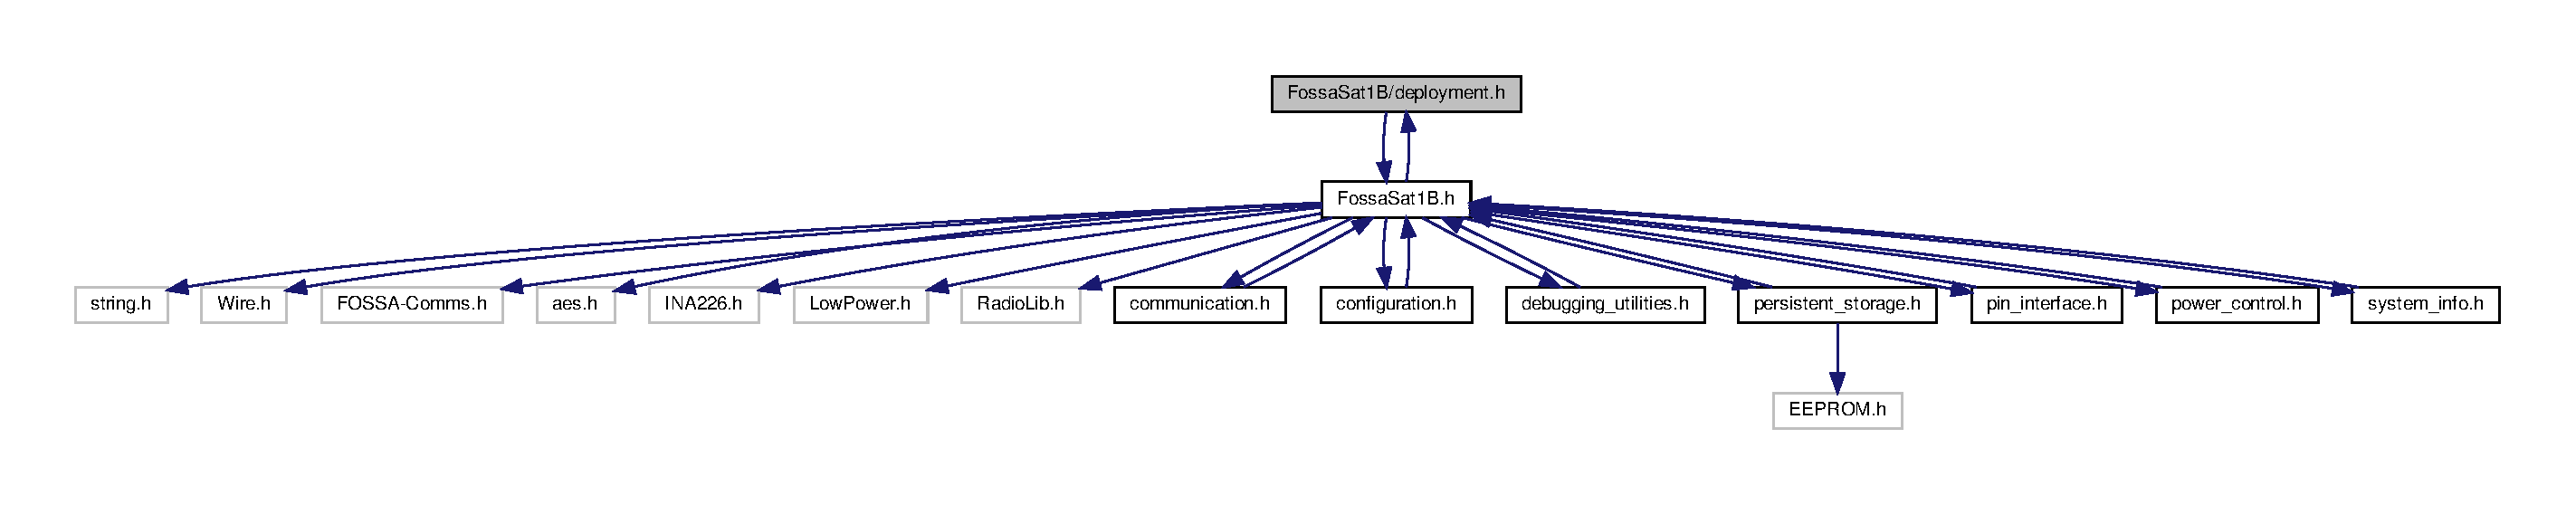
\includegraphics[width=350pt]{deployment_8h__incl}
\end{center}
\end{figure}
This graph shows which files directly or indirectly include this file\+:
\nopagebreak
\begin{figure}[H]
\begin{center}
\leavevmode
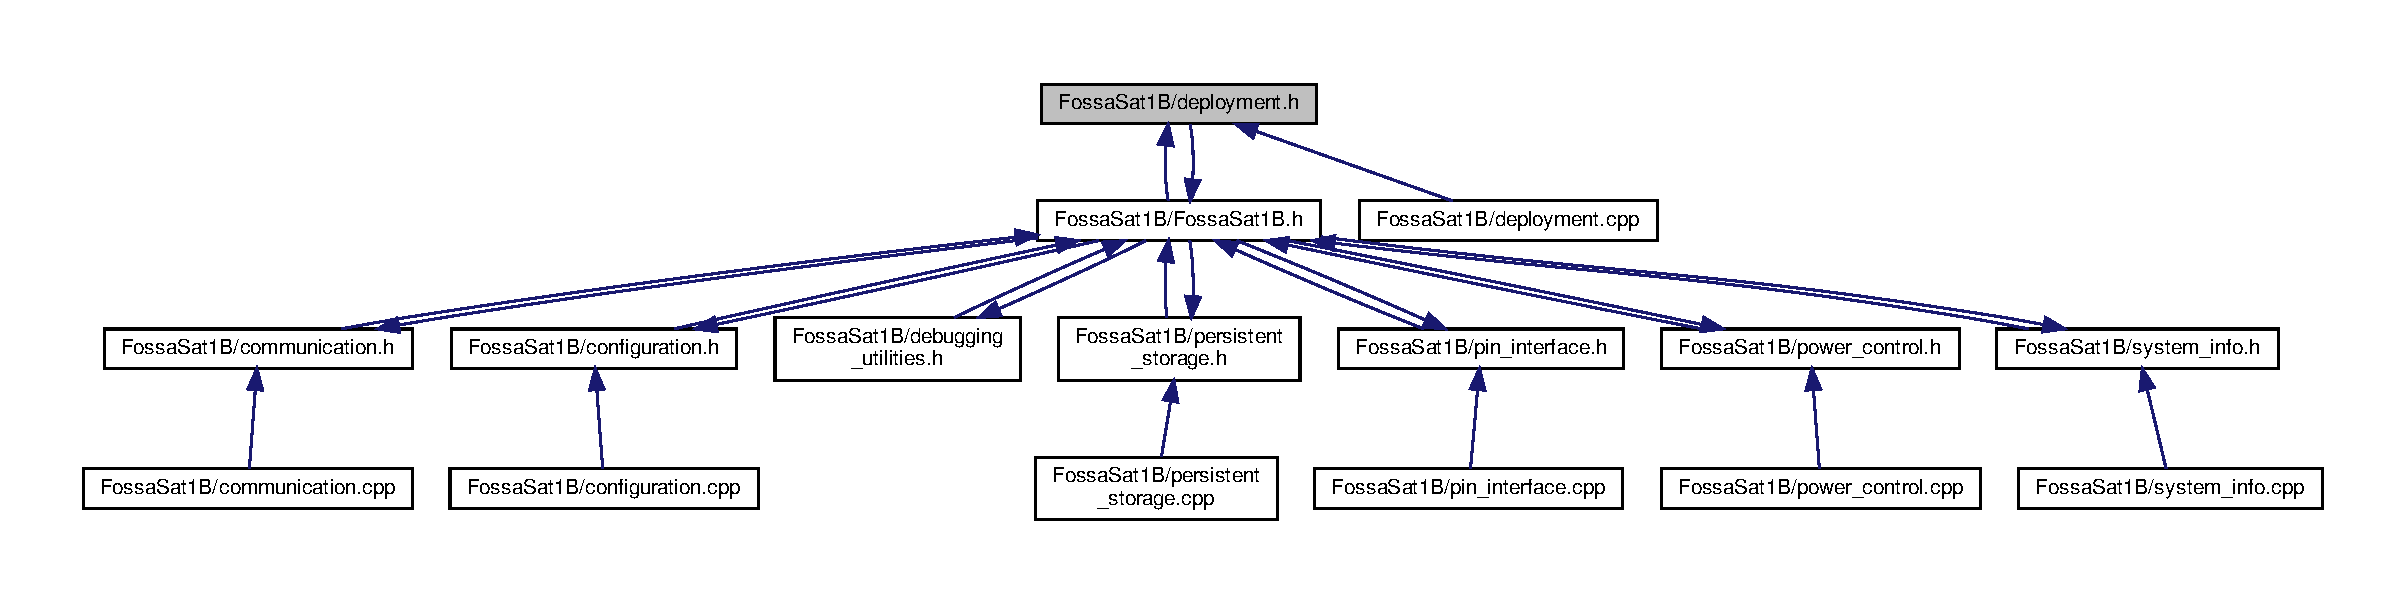
\includegraphics[width=350pt]{deployment_8h__dep__incl}
\end{center}
\end{figure}
\subsection*{Functions}
\begin{DoxyCompactItemize}
\item 
void \hyperlink{deployment_8h_acf81803b5f0482964a9c550f249fc3cf}{Deployment\+\_\+\+Deploy} ()
\begin{DoxyCompactList}\small\item\em This function deploys the antenna by powering the M\+O\+S\+F\+E\+T1/2 for 1200 seconds. \end{DoxyCompactList}\end{DoxyCompactItemize}


\subsection{Detailed Description}
The deployment sequence is outlined in the source \hyperlink{deployment_8cpp_source}{deployment.\+cpp}. 



\subsection{Function Documentation}
\mbox{\Hypertarget{deployment_8h_acf81803b5f0482964a9c550f249fc3cf}\label{deployment_8h_acf81803b5f0482964a9c550f249fc3cf}} 
\index{deployment.\+h@{deployment.\+h}!Deployment\+\_\+\+Deploy@{Deployment\+\_\+\+Deploy}}
\index{Deployment\+\_\+\+Deploy@{Deployment\+\_\+\+Deploy}!deployment.\+h@{deployment.\+h}}
\subsubsection{\texorpdfstring{Deployment\+\_\+\+Deploy()}{Deployment\_Deploy()}}
{\footnotesize\ttfamily void Deployment\+\_\+\+Deploy (\begin{DoxyParamCaption}{ }\end{DoxyParamCaption})}



This function deploys the antenna by powering the M\+O\+S\+F\+E\+T1/2 for 1200 seconds. 

\begin{DoxyRefDesc}{Test}
\item[\hyperlink{test__test000031}{Test}](ID D\+E\+P\+L\+O\+Y\+M\+E\+N\+T\+\_\+\+H\+\_\+\+T0) (S\+EV 1) Make sure the antenna deploys using this function.\end{DoxyRefDesc}


Definition at line 3 of file deployment.\+cpp.


\hypertarget{persistent__storage_8h}{}\section{Fossa\+Sat1\+B/persistent\+\_\+storage.h File Reference}
\label{persistent__storage_8h}\index{Fossa\+Sat1\+B/persistent\+\_\+storage.\+h@{Fossa\+Sat1\+B/persistent\+\_\+storage.\+h}}


This module controls access to the E\+E\+P\+R\+OM.  


{\ttfamily \#include \char`\"{}Fossa\+Sat1\+B.\+h\char`\"{}}\newline
{\ttfamily \#include $<$E\+E\+P\+R\+O\+M.\+h$>$}\newline
Include dependency graph for persistent\+\_\+storage.\+h\+:
\nopagebreak
\begin{figure}[H]
\begin{center}
\leavevmode
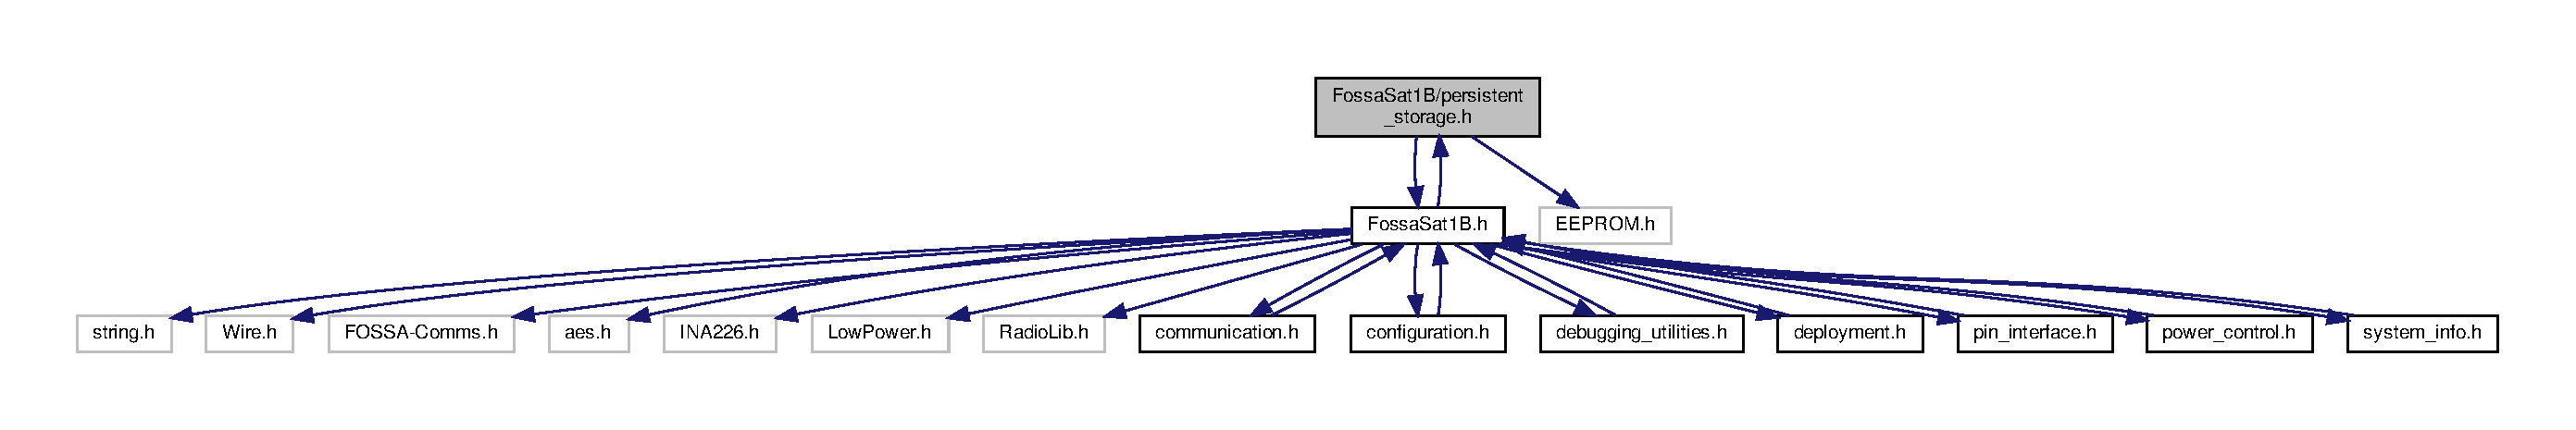
\includegraphics[width=350pt]{persistent__storage_8h__incl}
\end{center}
\end{figure}
This graph shows which files directly or indirectly include this file\+:
\nopagebreak
\begin{figure}[H]
\begin{center}
\leavevmode
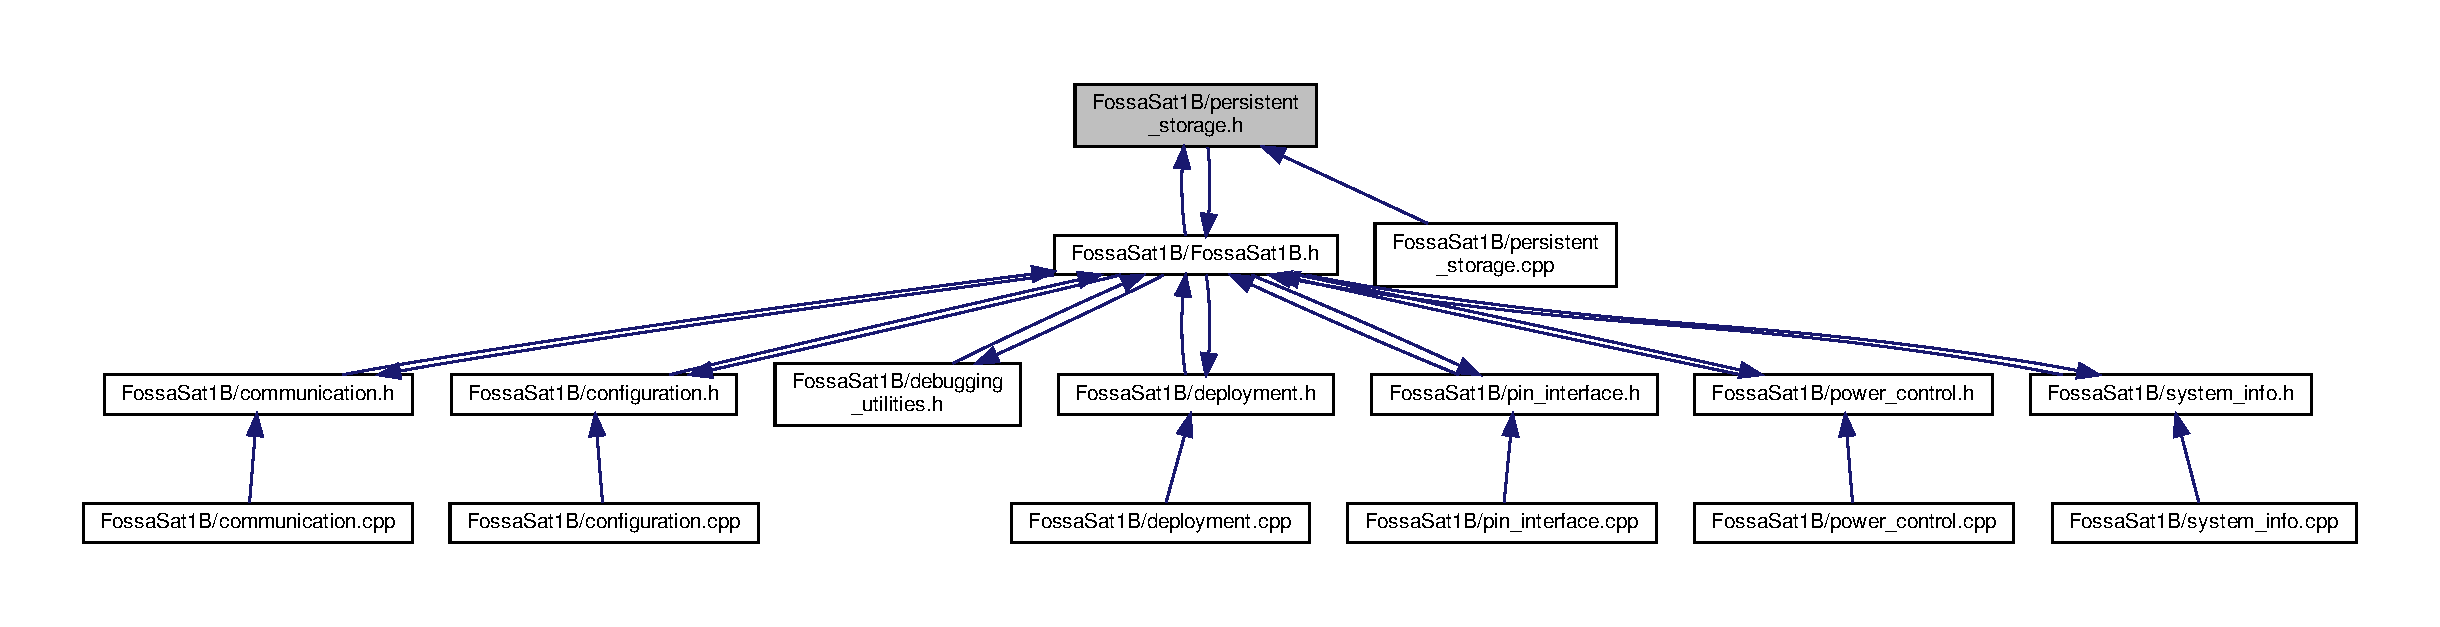
\includegraphics[width=350pt]{persistent__storage_8h__dep__incl}
\end{center}
\end{figure}
\subsection*{Functions}
\begin{DoxyCompactItemize}
\item 
{\footnotesize template$<$typename T $>$ }\\T \hyperlink{persistent__storage_8h_a188438a1c042e8a73932cab87f5b66ec}{Persistent\+\_\+\+Storage\+\_\+\+Read} (uint16\+\_\+t addr)
\begin{DoxyCompactList}\small\item\em This function reads a value of type T from E\+E\+P\+R\+OM. \end{DoxyCompactList}\item 
{\footnotesize template$<$typename T $>$ }\\void \hyperlink{persistent__storage_8h_aca7da667eec4409f7001ef618fa2c4b9}{Persistent\+\_\+\+Storage\+\_\+\+Write} (uint16\+\_\+t addr, T val)
\begin{DoxyCompactList}\small\item\em This function writes a value of type T to the eerom. \end{DoxyCompactList}\item 
void \hyperlink{persistent__storage_8h_a639d33b8a97eee3ccfaf9b7c00537cac}{Persistent\+\_\+\+Storage\+\_\+\+Wipe} ()
\begin{DoxyCompactList}\small\item\em This functions clears the E\+E\+P\+R\+OM by writing E\+E\+P\+R\+O\+M\+\_\+\+R\+E\+S\+E\+T\+\_\+\+V\+A\+L\+UE to each memory addres. \end{DoxyCompactList}\item 
void \hyperlink{persistent__storage_8h_a9642a7f1814ac81a5cc2b8b0a818aaba}{Persistent\+\_\+\+Storage\+\_\+\+Increment\+\_\+\+Counter} (uint16\+\_\+t addr)
\begin{DoxyCompactList}\small\item\em This functions increments 2-\/byte counter in E\+E\+P\+R\+OM. \end{DoxyCompactList}\item 
void \hyperlink{persistent__storage_8h_a7ca0126c55391f2e2c48dc1bd4af4c9a}{Persistent\+\_\+\+Storage\+\_\+\+Increment\+\_\+\+Frame\+\_\+\+Counter} (bool valid)
\begin{DoxyCompactList}\small\item\em This functions increments one of frame counters of the currently active modem in E\+E\+P\+R\+OM. \end{DoxyCompactList}\item 
{\footnotesize template$<$typename T $>$ }\\void \hyperlink{persistent__storage_8h_aa4b2798d95c617815859a53d38b20f16}{Persistent\+\_\+\+Storage\+\_\+\+Update\+\_\+\+Stats} (uint16\+\_\+t addr, T val)
\begin{DoxyCompactList}\small\item\em Updates minimum, average and maximum stats in E\+E\+P\+R\+OM. \end{DoxyCompactList}\end{DoxyCompactItemize}


\subsection{Detailed Description}
This module controls access to the E\+E\+P\+R\+OM. 



\subsection{Function Documentation}
\mbox{\Hypertarget{persistent__storage_8h_a9642a7f1814ac81a5cc2b8b0a818aaba}\label{persistent__storage_8h_a9642a7f1814ac81a5cc2b8b0a818aaba}} 
\index{persistent\+\_\+storage.\+h@{persistent\+\_\+storage.\+h}!Persistent\+\_\+\+Storage\+\_\+\+Increment\+\_\+\+Counter@{Persistent\+\_\+\+Storage\+\_\+\+Increment\+\_\+\+Counter}}
\index{Persistent\+\_\+\+Storage\+\_\+\+Increment\+\_\+\+Counter@{Persistent\+\_\+\+Storage\+\_\+\+Increment\+\_\+\+Counter}!persistent\+\_\+storage.\+h@{persistent\+\_\+storage.\+h}}
\subsubsection{\texorpdfstring{Persistent\+\_\+\+Storage\+\_\+\+Increment\+\_\+\+Counter()}{Persistent\_Storage\_Increment\_Counter()}}
{\footnotesize\ttfamily void Persistent\+\_\+\+Storage\+\_\+\+Increment\+\_\+\+Counter (\begin{DoxyParamCaption}\item[{uint16\+\_\+t}]{addr }\end{DoxyParamCaption})}



This functions increments 2-\/byte counter in E\+E\+P\+R\+OM. 


\begin{DoxyParams}{Parameters}
{\em addr} & The address of counter to increment \\
\hline
\end{DoxyParams}


Definition at line 55 of file persistent\+\_\+storage.\+cpp.

Here is the caller graph for this function\+:
\nopagebreak
\begin{figure}[H]
\begin{center}
\leavevmode
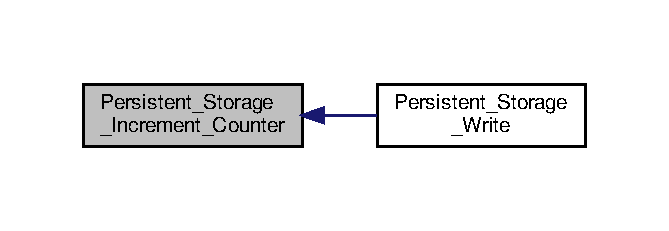
\includegraphics[width=321pt]{persistent__storage_8h_a9642a7f1814ac81a5cc2b8b0a818aaba_icgraph}
\end{center}
\end{figure}
\mbox{\Hypertarget{persistent__storage_8h_a7ca0126c55391f2e2c48dc1bd4af4c9a}\label{persistent__storage_8h_a7ca0126c55391f2e2c48dc1bd4af4c9a}} 
\index{persistent\+\_\+storage.\+h@{persistent\+\_\+storage.\+h}!Persistent\+\_\+\+Storage\+\_\+\+Increment\+\_\+\+Frame\+\_\+\+Counter@{Persistent\+\_\+\+Storage\+\_\+\+Increment\+\_\+\+Frame\+\_\+\+Counter}}
\index{Persistent\+\_\+\+Storage\+\_\+\+Increment\+\_\+\+Frame\+\_\+\+Counter@{Persistent\+\_\+\+Storage\+\_\+\+Increment\+\_\+\+Frame\+\_\+\+Counter}!persistent\+\_\+storage.\+h@{persistent\+\_\+storage.\+h}}
\subsubsection{\texorpdfstring{Persistent\+\_\+\+Storage\+\_\+\+Increment\+\_\+\+Frame\+\_\+\+Counter()}{Persistent\_Storage\_Increment\_Frame\_Counter()}}
{\footnotesize\ttfamily void Persistent\+\_\+\+Storage\+\_\+\+Increment\+\_\+\+Frame\+\_\+\+Counter (\begin{DoxyParamCaption}\item[{bool}]{valid }\end{DoxyParamCaption})}



This functions increments one of frame counters of the currently active modem in E\+E\+P\+R\+OM. 


\begin{DoxyParams}{Parameters}
{\em valid} & Whether to increment valid or invalid counter \\
\hline
\end{DoxyParams}


Definition at line 59 of file persistent\+\_\+storage.\+cpp.

Here is the caller graph for this function\+:
\nopagebreak
\begin{figure}[H]
\begin{center}
\leavevmode
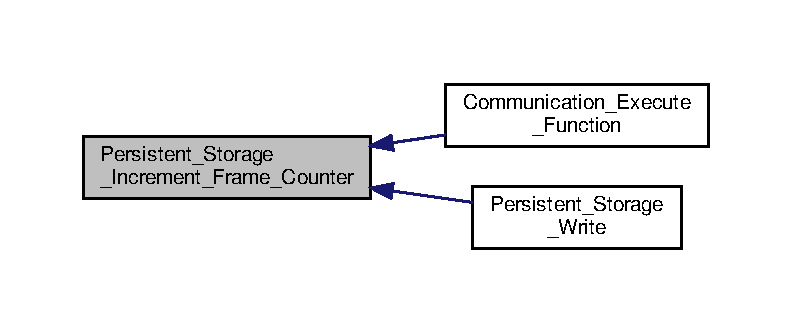
\includegraphics[width=350pt]{persistent__storage_8h_a7ca0126c55391f2e2c48dc1bd4af4c9a_icgraph}
\end{center}
\end{figure}
\mbox{\Hypertarget{persistent__storage_8h_a188438a1c042e8a73932cab87f5b66ec}\label{persistent__storage_8h_a188438a1c042e8a73932cab87f5b66ec}} 
\index{persistent\+\_\+storage.\+h@{persistent\+\_\+storage.\+h}!Persistent\+\_\+\+Storage\+\_\+\+Read@{Persistent\+\_\+\+Storage\+\_\+\+Read}}
\index{Persistent\+\_\+\+Storage\+\_\+\+Read@{Persistent\+\_\+\+Storage\+\_\+\+Read}!persistent\+\_\+storage.\+h@{persistent\+\_\+storage.\+h}}
\subsubsection{\texorpdfstring{Persistent\+\_\+\+Storage\+\_\+\+Read()}{Persistent\_Storage\_Read()}}
{\footnotesize\ttfamily template$<$typename T $>$ \\
T Persistent\+\_\+\+Storage\+\_\+\+Read (\begin{DoxyParamCaption}\item[{uint16\+\_\+t}]{addr }\end{DoxyParamCaption})}



This function reads a value of type T from E\+E\+P\+R\+OM. 


\begin{DoxyTemplParams}{Template Parameters}
{\em T} & \\
\hline
\end{DoxyTemplParams}

\begin{DoxyParams}{Parameters}
{\em addr} & Memory address. \\
\hline
\end{DoxyParams}
\begin{DoxyReturn}{Returns}
T 
\end{DoxyReturn}


Definition at line 22 of file persistent\+\_\+storage.\+h.

\mbox{\Hypertarget{persistent__storage_8h_aa4b2798d95c617815859a53d38b20f16}\label{persistent__storage_8h_aa4b2798d95c617815859a53d38b20f16}} 
\index{persistent\+\_\+storage.\+h@{persistent\+\_\+storage.\+h}!Persistent\+\_\+\+Storage\+\_\+\+Update\+\_\+\+Stats@{Persistent\+\_\+\+Storage\+\_\+\+Update\+\_\+\+Stats}}
\index{Persistent\+\_\+\+Storage\+\_\+\+Update\+\_\+\+Stats@{Persistent\+\_\+\+Storage\+\_\+\+Update\+\_\+\+Stats}!persistent\+\_\+storage.\+h@{persistent\+\_\+storage.\+h}}
\subsubsection{\texorpdfstring{Persistent\+\_\+\+Storage\+\_\+\+Update\+\_\+\+Stats()}{Persistent\_Storage\_Update\_Stats()}}
{\footnotesize\ttfamily template$<$typename T $>$ \\
void Persistent\+\_\+\+Storage\+\_\+\+Update\+\_\+\+Stats (\begin{DoxyParamCaption}\item[{uint16\+\_\+t}]{addr,  }\item[{T}]{val }\end{DoxyParamCaption})}



Updates minimum, average and maximum stats in E\+E\+P\+R\+OM. 


\begin{DoxyTemplParams}{Template Parameters}
{\em T} & \\
\hline
\end{DoxyTemplParams}

\begin{DoxyParams}{Parameters}
{\em addr} & Memory address. \\
\hline
{\em val} & \\
\hline
\end{DoxyParams}


Definition at line 73 of file persistent\+\_\+storage.\+h.

\mbox{\Hypertarget{persistent__storage_8h_a639d33b8a97eee3ccfaf9b7c00537cac}\label{persistent__storage_8h_a639d33b8a97eee3ccfaf9b7c00537cac}} 
\index{persistent\+\_\+storage.\+h@{persistent\+\_\+storage.\+h}!Persistent\+\_\+\+Storage\+\_\+\+Wipe@{Persistent\+\_\+\+Storage\+\_\+\+Wipe}}
\index{Persistent\+\_\+\+Storage\+\_\+\+Wipe@{Persistent\+\_\+\+Storage\+\_\+\+Wipe}!persistent\+\_\+storage.\+h@{persistent\+\_\+storage.\+h}}
\subsubsection{\texorpdfstring{Persistent\+\_\+\+Storage\+\_\+\+Wipe()}{Persistent\_Storage\_Wipe()}}
{\footnotesize\ttfamily void Persistent\+\_\+\+Storage\+\_\+\+Wipe (\begin{DoxyParamCaption}{ }\end{DoxyParamCaption})}



This functions clears the E\+E\+P\+R\+OM by writing E\+E\+P\+R\+O\+M\+\_\+\+R\+E\+S\+E\+T\+\_\+\+V\+A\+L\+UE to each memory addres. 

\begin{DoxyRefDesc}{Test}
\item[\hyperlink{test__test000032}{Test}](ID P\+E\+R\+S\+I\+S\+\_\+\+S\+T\+O\+R\+\_\+\+H\+\_\+\+T0) (S\+EV 1) Does the E\+E\+P\+R\+OM enter a valid state after this function is ran?\end{DoxyRefDesc}


Definition at line 3 of file persistent\+\_\+storage.\+cpp.

Here is the caller graph for this function\+:
\nopagebreak
\begin{figure}[H]
\begin{center}
\leavevmode
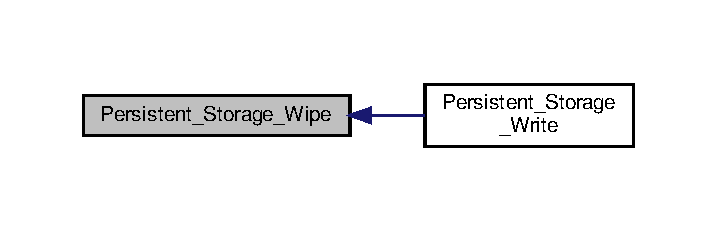
\includegraphics[width=344pt]{persistent__storage_8h_a639d33b8a97eee3ccfaf9b7c00537cac_icgraph}
\end{center}
\end{figure}
\mbox{\Hypertarget{persistent__storage_8h_aca7da667eec4409f7001ef618fa2c4b9}\label{persistent__storage_8h_aca7da667eec4409f7001ef618fa2c4b9}} 
\index{persistent\+\_\+storage.\+h@{persistent\+\_\+storage.\+h}!Persistent\+\_\+\+Storage\+\_\+\+Write@{Persistent\+\_\+\+Storage\+\_\+\+Write}}
\index{Persistent\+\_\+\+Storage\+\_\+\+Write@{Persistent\+\_\+\+Storage\+\_\+\+Write}!persistent\+\_\+storage.\+h@{persistent\+\_\+storage.\+h}}
\subsubsection{\texorpdfstring{Persistent\+\_\+\+Storage\+\_\+\+Write()}{Persistent\_Storage\_Write()}}
{\footnotesize\ttfamily template$<$typename T $>$ \\
void Persistent\+\_\+\+Storage\+\_\+\+Write (\begin{DoxyParamCaption}\item[{uint16\+\_\+t}]{addr,  }\item[{T}]{val }\end{DoxyParamCaption})}



This function writes a value of type T to the eerom. 


\begin{DoxyTemplParams}{Template Parameters}
{\em T} & \\
\hline
\end{DoxyTemplParams}

\begin{DoxyParams}{Parameters}
{\em addr} & Memory address. \\
\hline
{\em val} & \\
\hline
\end{DoxyParams}


Definition at line 36 of file persistent\+\_\+storage.\+h.

Here is the call graph for this function\+:
\nopagebreak
\begin{figure}[H]
\begin{center}
\leavevmode
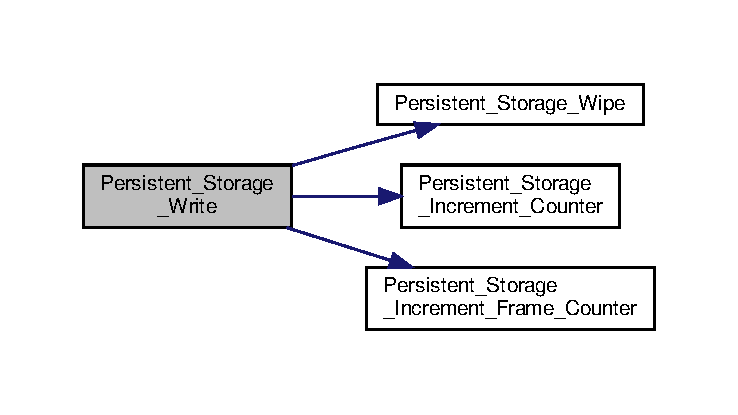
\includegraphics[width=350pt]{persistent__storage_8h_aca7da667eec4409f7001ef618fa2c4b9_cgraph}
\end{center}
\end{figure}

\hypertarget{pin__interface_8h}{}\section{Fossa\+Sat1\+B/pin\+\_\+interface.h File Reference}
\label{pin__interface_8h}\index{Fossa\+Sat1\+B/pin\+\_\+interface.\+h@{Fossa\+Sat1\+B/pin\+\_\+interface.\+h}}


This module controls access to the components connect to via pins.  


{\ttfamily \#include \char`\"{}Fossa\+Sat1\+B.\+h\char`\"{}}\newline
Include dependency graph for pin\+\_\+interface.\+h\+:
\nopagebreak
\begin{figure}[H]
\begin{center}
\leavevmode
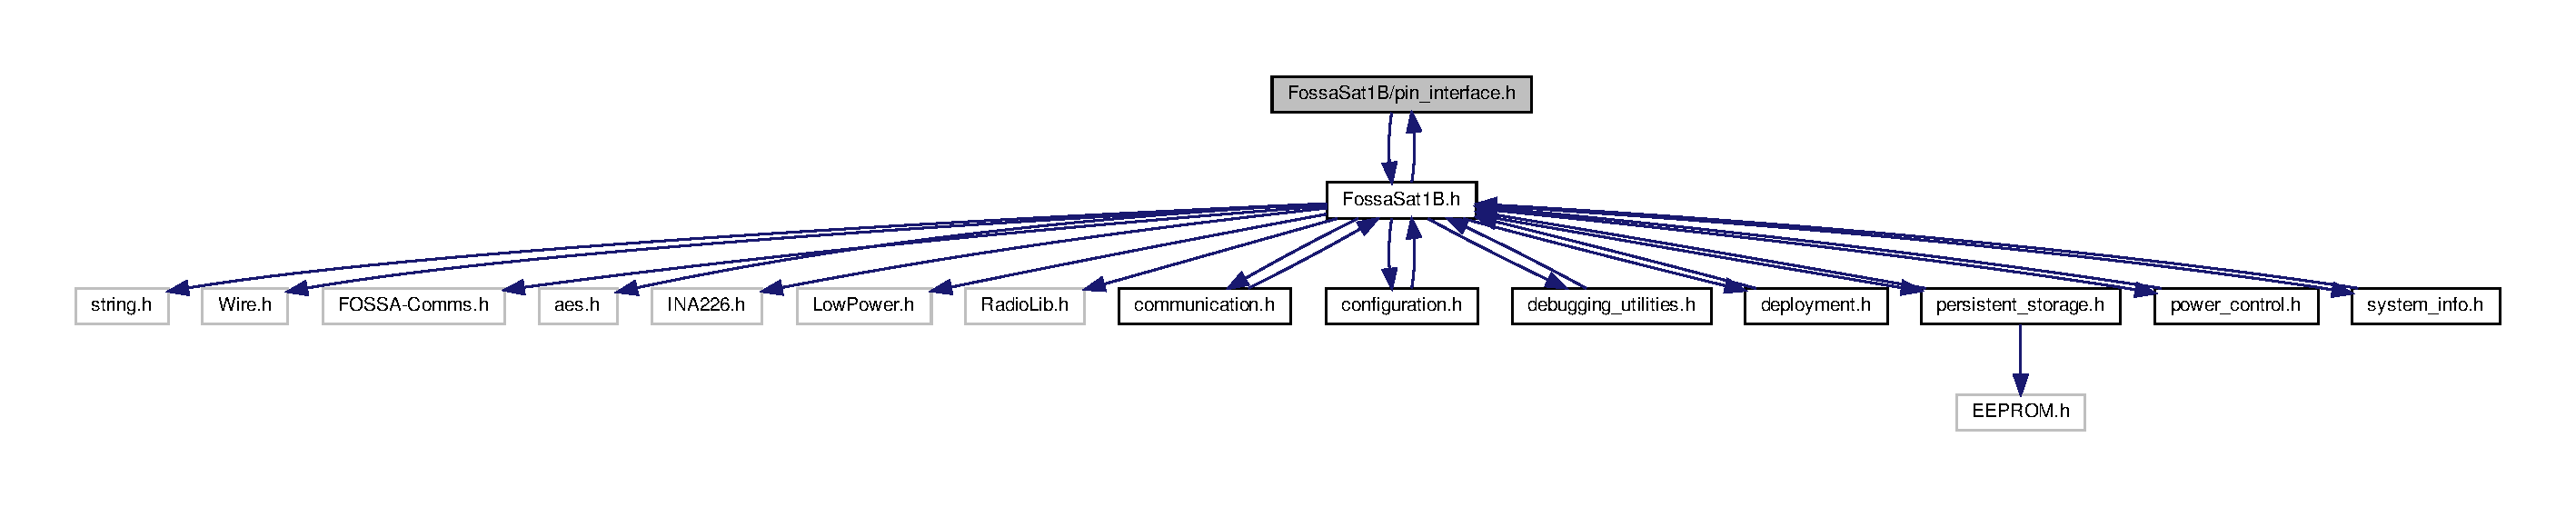
\includegraphics[width=350pt]{pin__interface_8h__incl}
\end{center}
\end{figure}
This graph shows which files directly or indirectly include this file\+:
\nopagebreak
\begin{figure}[H]
\begin{center}
\leavevmode
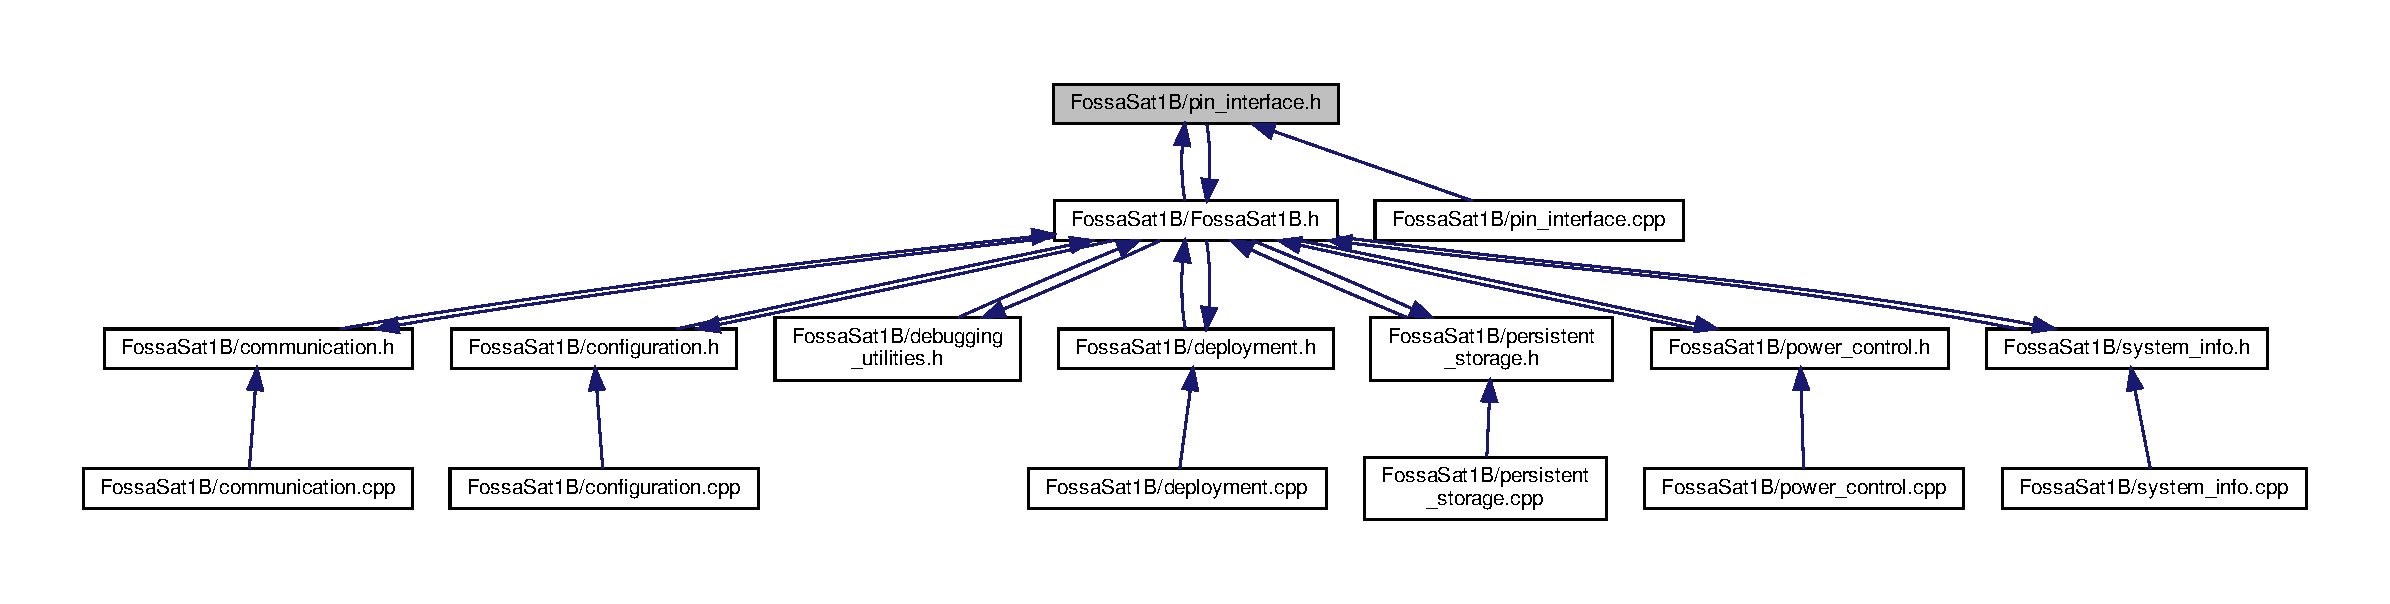
\includegraphics[width=350pt]{pin__interface_8h__dep__incl}
\end{center}
\end{figure}
\subsection*{Functions}
\begin{DoxyCompactItemize}
\item 
void \hyperlink{pin__interface_8h_a5f7aaf72d73969a1623da04d35f6f98c}{Pin\+\_\+\+Interface\+\_\+\+Set\+\_\+\+Temp\+\_\+\+Resolution} (uint8\+\_\+t sensor\+Addr, uint8\+\_\+t res)
\begin{DoxyCompactList}\small\item\em This function sets the resolution of the T\+M\+P100. \end{DoxyCompactList}\item 
float \hyperlink{pin__interface_8h_a19d8eea2c4cc2711fb370569770ea4e7}{Pin\+\_\+\+Interface\+\_\+\+Read\+\_\+\+Temperature} (uint8\+\_\+t sensor\+Addr)
\begin{DoxyCompactList}\small\item\em This function reads the T\+M\+P100\textquotesingle{}s value from its wire address. \end{DoxyCompactList}\item 
int8\+\_\+t \hyperlink{pin__interface_8h_ad2aae71d01b9b9cdf1f12cb22b820781}{Pin\+\_\+\+Interface\+\_\+\+Read\+\_\+\+Temperature\+\_\+\+Internal} ()
\begin{DoxyCompactList}\small\item\em This function reads the M\+CU\textquotesingle{}s internal temperature. \end{DoxyCompactList}\item 
float \hyperlink{pin__interface_8h_a33980455d0d1f81544f71605e4acaba5}{Pin\+\_\+\+Interface\+\_\+\+Read\+\_\+\+Voltage} (uint8\+\_\+t pin)
\begin{DoxyCompactList}\small\item\em Read the voltage of a given pin. \end{DoxyCompactList}\item 
void \hyperlink{pin__interface_8h_a912aff671fe4db53ca23520a1d203d6f}{Pin\+\_\+\+Interface\+\_\+\+Watchdog\+\_\+\+Heartbeat} (bool manage\+Battery=false)
\begin{DoxyCompactList}\small\item\em This function toggles the signal to the watchdog and writes it to the pin. \end{DoxyCompactList}\item 
void \hyperlink{pin__interface_8h_a016ad19733549152625049452a9c01ca}{Pin\+\_\+\+Interface\+\_\+\+Watchdog\+\_\+\+Restart} ()
\begin{DoxyCompactList}\small\item\em Restarts the watchdog. \end{DoxyCompactList}\end{DoxyCompactItemize}


\subsection{Detailed Description}
This module controls access to the components connect to via pins. 



\subsection{Function Documentation}
\mbox{\Hypertarget{pin__interface_8h_a19d8eea2c4cc2711fb370569770ea4e7}\label{pin__interface_8h_a19d8eea2c4cc2711fb370569770ea4e7}} 
\index{pin\+\_\+interface.\+h@{pin\+\_\+interface.\+h}!Pin\+\_\+\+Interface\+\_\+\+Read\+\_\+\+Temperature@{Pin\+\_\+\+Interface\+\_\+\+Read\+\_\+\+Temperature}}
\index{Pin\+\_\+\+Interface\+\_\+\+Read\+\_\+\+Temperature@{Pin\+\_\+\+Interface\+\_\+\+Read\+\_\+\+Temperature}!pin\+\_\+interface.\+h@{pin\+\_\+interface.\+h}}
\subsubsection{\texorpdfstring{Pin\+\_\+\+Interface\+\_\+\+Read\+\_\+\+Temperature()}{Pin\_Interface\_Read\_Temperature()}}
{\footnotesize\ttfamily float Pin\+\_\+\+Interface\+\_\+\+Read\+\_\+\+Temperature (\begin{DoxyParamCaption}\item[{uint8\+\_\+t}]{sensor\+Addr }\end{DoxyParamCaption})}



This function reads the T\+M\+P100\textquotesingle{}s value from its wire address. 

\begin{DoxyRefDesc}{Test}
\item[\hyperlink{test__test000034}{Test}](ID P\+I\+N\+\_\+\+I\+N\+T\+E\+R\+F\+\_\+\+H\+\_\+\+T1) (S\+EV 1) Make sure that all resolutions do not break the satellite. 

(ID P\+I\+N\+\_\+\+I\+N\+T\+E\+R\+F\+\_\+\+H\+\_\+\+T2) (S\+EV 1) Make sure this returns the correct value.\end{DoxyRefDesc}



\begin{DoxyParams}{Parameters}
{\em sensor\+Addr} & Wire address of the T\+M\+P100 \\
\hline
\end{DoxyParams}
\begin{DoxyReturn}{Returns}
float The temperature value in Degrees C at the specified resolution. 
\end{DoxyReturn}


Definition at line 16 of file pin\+\_\+interface.\+cpp.

\mbox{\Hypertarget{pin__interface_8h_ad2aae71d01b9b9cdf1f12cb22b820781}\label{pin__interface_8h_ad2aae71d01b9b9cdf1f12cb22b820781}} 
\index{pin\+\_\+interface.\+h@{pin\+\_\+interface.\+h}!Pin\+\_\+\+Interface\+\_\+\+Read\+\_\+\+Temperature\+\_\+\+Internal@{Pin\+\_\+\+Interface\+\_\+\+Read\+\_\+\+Temperature\+\_\+\+Internal}}
\index{Pin\+\_\+\+Interface\+\_\+\+Read\+\_\+\+Temperature\+\_\+\+Internal@{Pin\+\_\+\+Interface\+\_\+\+Read\+\_\+\+Temperature\+\_\+\+Internal}!pin\+\_\+interface.\+h@{pin\+\_\+interface.\+h}}
\subsubsection{\texorpdfstring{Pin\+\_\+\+Interface\+\_\+\+Read\+\_\+\+Temperature\+\_\+\+Internal()}{Pin\_Interface\_Read\_Temperature\_Internal()}}
{\footnotesize\ttfamily int8\+\_\+t Pin\+\_\+\+Interface\+\_\+\+Read\+\_\+\+Temperature\+\_\+\+Internal (\begin{DoxyParamCaption}{ }\end{DoxyParamCaption})}



This function reads the M\+CU\textquotesingle{}s internal temperature. 

\begin{DoxyRefDesc}{Test}
\item[\hyperlink{test__test000035}{Test}](ID P\+I\+N\+\_\+\+I\+N\+T\+E\+R\+F\+\_\+\+H\+\_\+\+T3) (S\+EV 1) Make sure this does not break the satellite. 

(ID P\+I\+N\+\_\+\+I\+N\+T\+E\+R\+F\+\_\+\+H\+\_\+\+T4) (S\+EV 2) Make sure this returns the correct value.\end{DoxyRefDesc}


\begin{DoxyReturn}{Returns}
int8\+\_\+t The temperature returned by the M\+CU in Degrees C. 
\end{DoxyReturn}


Definition at line 28 of file pin\+\_\+interface.\+cpp.

\mbox{\Hypertarget{pin__interface_8h_a33980455d0d1f81544f71605e4acaba5}\label{pin__interface_8h_a33980455d0d1f81544f71605e4acaba5}} 
\index{pin\+\_\+interface.\+h@{pin\+\_\+interface.\+h}!Pin\+\_\+\+Interface\+\_\+\+Read\+\_\+\+Voltage@{Pin\+\_\+\+Interface\+\_\+\+Read\+\_\+\+Voltage}}
\index{Pin\+\_\+\+Interface\+\_\+\+Read\+\_\+\+Voltage@{Pin\+\_\+\+Interface\+\_\+\+Read\+\_\+\+Voltage}!pin\+\_\+interface.\+h@{pin\+\_\+interface.\+h}}
\subsubsection{\texorpdfstring{Pin\+\_\+\+Interface\+\_\+\+Read\+\_\+\+Voltage()}{Pin\_Interface\_Read\_Voltage()}}
{\footnotesize\ttfamily float Pin\+\_\+\+Interface\+\_\+\+Read\+\_\+\+Voltage (\begin{DoxyParamCaption}\item[{uint8\+\_\+t}]{pin }\end{DoxyParamCaption})}



Read the voltage of a given pin. 

\begin{DoxyRefDesc}{Test}
\item[\hyperlink{test__test000036}{Test}](ID P\+I\+N\+\_\+\+I\+N\+T\+E\+R\+F\+\_\+\+H\+\_\+\+T5) (S\+EV 1) Make sure the given equation is correct for all compatable pins.\end{DoxyRefDesc}



\begin{DoxyParams}{Parameters}
{\em pin} & The pin to read from. \\
\hline
\end{DoxyParams}
\begin{DoxyReturn}{Returns}
float The voltage. 
\end{DoxyReturn}


Definition at line 43 of file pin\+\_\+interface.\+cpp.

\mbox{\Hypertarget{pin__interface_8h_a5f7aaf72d73969a1623da04d35f6f98c}\label{pin__interface_8h_a5f7aaf72d73969a1623da04d35f6f98c}} 
\index{pin\+\_\+interface.\+h@{pin\+\_\+interface.\+h}!Pin\+\_\+\+Interface\+\_\+\+Set\+\_\+\+Temp\+\_\+\+Resolution@{Pin\+\_\+\+Interface\+\_\+\+Set\+\_\+\+Temp\+\_\+\+Resolution}}
\index{Pin\+\_\+\+Interface\+\_\+\+Set\+\_\+\+Temp\+\_\+\+Resolution@{Pin\+\_\+\+Interface\+\_\+\+Set\+\_\+\+Temp\+\_\+\+Resolution}!pin\+\_\+interface.\+h@{pin\+\_\+interface.\+h}}
\subsubsection{\texorpdfstring{Pin\+\_\+\+Interface\+\_\+\+Set\+\_\+\+Temp\+\_\+\+Resolution()}{Pin\_Interface\_Set\_Temp\_Resolution()}}
{\footnotesize\ttfamily void Pin\+\_\+\+Interface\+\_\+\+Set\+\_\+\+Temp\+\_\+\+Resolution (\begin{DoxyParamCaption}\item[{uint8\+\_\+t}]{sensor\+Addr,  }\item[{uint8\+\_\+t}]{res }\end{DoxyParamCaption})}



This function sets the resolution of the T\+M\+P100. 

\begin{DoxyRefDesc}{Test}
\item[\hyperlink{test__test000033}{Test}](ID P\+I\+N\+\_\+\+I\+N\+T\+E\+R\+F\+\_\+\+H\+\_\+\+T0) (S\+EV 1) Make sure that this does not break with the given resolutions.\end{DoxyRefDesc}



\begin{DoxyParams}{Parameters}
{\em sensor\+Addr} & Wire address of the T\+M\+P100. \\
\hline
{\em res} & The value that relates to the resolution property of the T\+M\+P100. See \hyperlink{group__defines__tmp100__configuration}{T\+M\+P100 Temperature Sensor Configuration} \\
\hline
\end{DoxyParams}


Definition at line 3 of file pin\+\_\+interface.\+cpp.

\mbox{\Hypertarget{pin__interface_8h_a912aff671fe4db53ca23520a1d203d6f}\label{pin__interface_8h_a912aff671fe4db53ca23520a1d203d6f}} 
\index{pin\+\_\+interface.\+h@{pin\+\_\+interface.\+h}!Pin\+\_\+\+Interface\+\_\+\+Watchdog\+\_\+\+Heartbeat@{Pin\+\_\+\+Interface\+\_\+\+Watchdog\+\_\+\+Heartbeat}}
\index{Pin\+\_\+\+Interface\+\_\+\+Watchdog\+\_\+\+Heartbeat@{Pin\+\_\+\+Interface\+\_\+\+Watchdog\+\_\+\+Heartbeat}!pin\+\_\+interface.\+h@{pin\+\_\+interface.\+h}}
\subsubsection{\texorpdfstring{Pin\+\_\+\+Interface\+\_\+\+Watchdog\+\_\+\+Heartbeat()}{Pin\_Interface\_Watchdog\_Heartbeat()}}
{\footnotesize\ttfamily void Pin\+\_\+\+Interface\+\_\+\+Watchdog\+\_\+\+Heartbeat (\begin{DoxyParamCaption}\item[{bool}]{manage\+Battery = {\ttfamily false} }\end{DoxyParamCaption})}



This function toggles the signal to the watchdog and writes it to the pin. 

\begin{DoxyRefDesc}{Test}
\item[\hyperlink{test__test000037}{Test}](ID P\+I\+N\+\_\+\+I\+N\+T\+E\+R\+F\+\_\+\+H\+\_\+\+T6) (S\+EV 1) Make sure this function keeps the satellite alive.\end{DoxyRefDesc}



\begin{DoxyParams}{Parameters}
{\em manage\+Battery} & Whether to perform battery and power management. \\
\hline
\end{DoxyParams}


Definition at line 48 of file pin\+\_\+interface.\+cpp.

Here is the call graph for this function\+:
\nopagebreak
\begin{figure}[H]
\begin{center}
\leavevmode
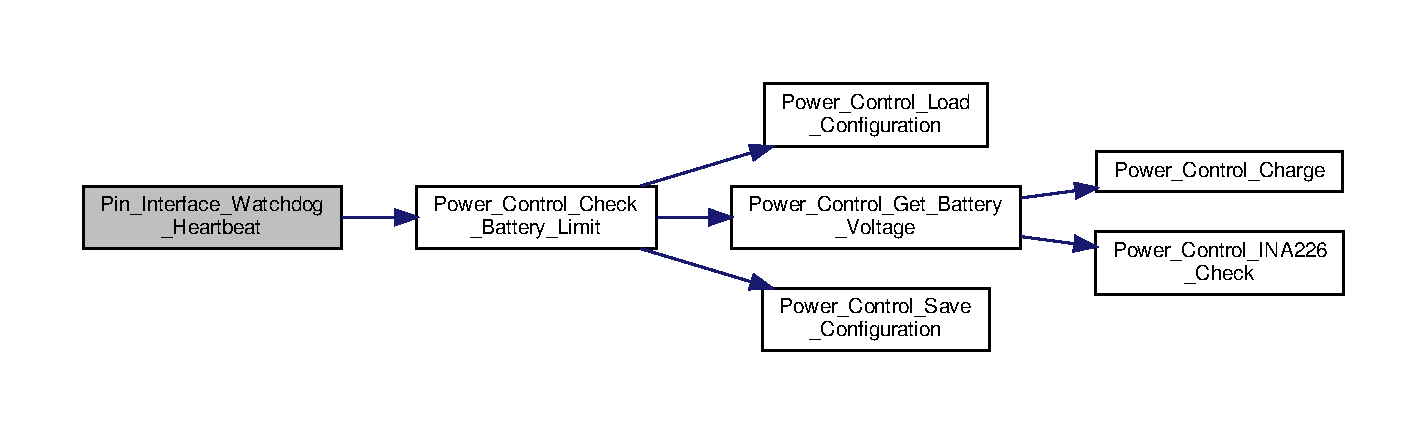
\includegraphics[width=350pt]{pin__interface_8h_a912aff671fe4db53ca23520a1d203d6f_cgraph}
\end{center}
\end{figure}
Here is the caller graph for this function\+:
\nopagebreak
\begin{figure}[H]
\begin{center}
\leavevmode
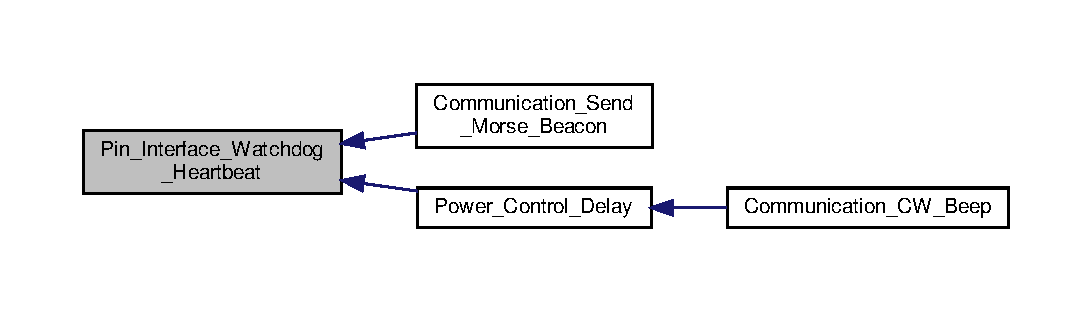
\includegraphics[width=350pt]{pin__interface_8h_a912aff671fe4db53ca23520a1d203d6f_icgraph}
\end{center}
\end{figure}
\mbox{\Hypertarget{pin__interface_8h_a016ad19733549152625049452a9c01ca}\label{pin__interface_8h_a016ad19733549152625049452a9c01ca}} 
\index{pin\+\_\+interface.\+h@{pin\+\_\+interface.\+h}!Pin\+\_\+\+Interface\+\_\+\+Watchdog\+\_\+\+Restart@{Pin\+\_\+\+Interface\+\_\+\+Watchdog\+\_\+\+Restart}}
\index{Pin\+\_\+\+Interface\+\_\+\+Watchdog\+\_\+\+Restart@{Pin\+\_\+\+Interface\+\_\+\+Watchdog\+\_\+\+Restart}!pin\+\_\+interface.\+h@{pin\+\_\+interface.\+h}}
\subsubsection{\texorpdfstring{Pin\+\_\+\+Interface\+\_\+\+Watchdog\+\_\+\+Restart()}{Pin\_Interface\_Watchdog\_Restart()}}
{\footnotesize\ttfamily void Pin\+\_\+\+Interface\+\_\+\+Watchdog\+\_\+\+Restart (\begin{DoxyParamCaption}{ }\end{DoxyParamCaption})}



Restarts the watchdog. 

\begin{DoxyRefDesc}{Test}
\item[\hyperlink{test__test000038}{Test}](ID P\+I\+N\+\_\+\+I\+N\+T\+E\+R\+F\+\_\+\+H\+\_\+\+T7) (S\+EV 1) Make sure this function resets the watchdog.\end{DoxyRefDesc}


Definition at line 58 of file pin\+\_\+interface.\+cpp.


\hypertarget{power__control_8h}{}\section{Fossa\+Sat1\+B/power\+\_\+control.h File Reference}
\label{power__control_8h}\index{Fossa\+Sat1\+B/power\+\_\+control.\+h@{Fossa\+Sat1\+B/power\+\_\+control.\+h}}
{\ttfamily \#include \char`\"{}Fossa\+Sat1\+B.\+h\char`\"{}}\newline
Include dependency graph for power\+\_\+control.\+h\+:
\nopagebreak
\begin{figure}[H]
\begin{center}
\leavevmode
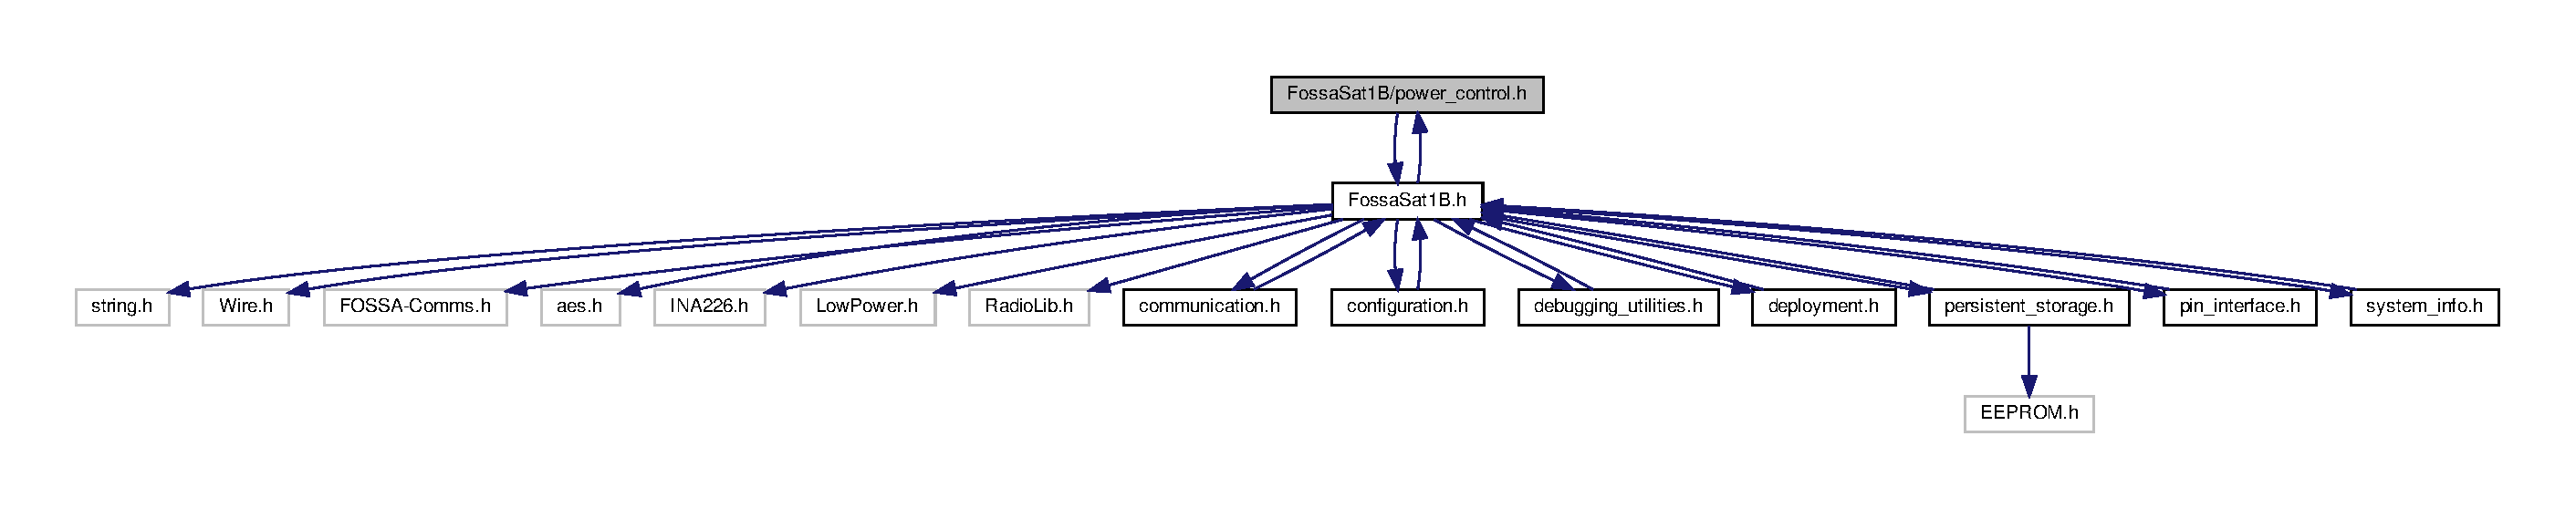
\includegraphics[width=350pt]{power__control_8h__incl}
\end{center}
\end{figure}
This graph shows which files directly or indirectly include this file\+:
\nopagebreak
\begin{figure}[H]
\begin{center}
\leavevmode
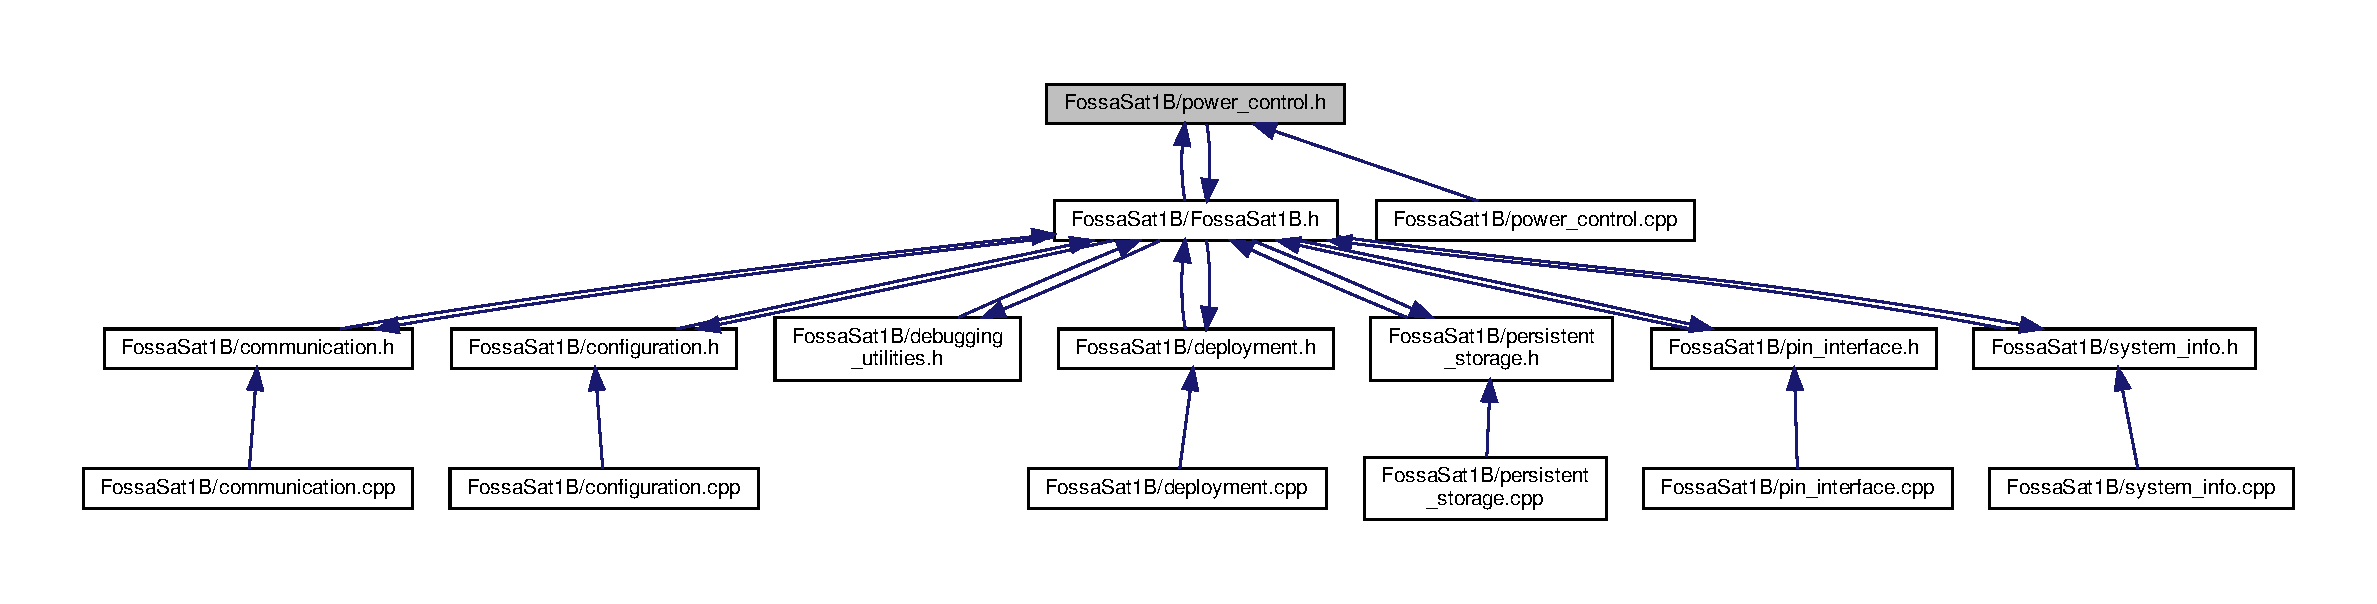
\includegraphics[width=350pt]{power__control_8h__dep__incl}
\end{center}
\end{figure}
\subsection*{Data Structures}
\begin{DoxyCompactItemize}
\item 
struct \hyperlink{structpower_config_bits__t}{power\+Config\+Bits\+\_\+t}
\begin{DoxyCompactList}\small\item\em Power configuration strutcture, each entry is one bit long. Total 1 byte, low\+Power\+Mode\+Active is the least significant bit. \end{DoxyCompactList}\item 
union \hyperlink{unionpower_config__t}{power\+Config\+\_\+t}
\begin{DoxyCompactList}\small\item\em Union to quickly access power configuration bits or the entire single-\/byte value. \end{DoxyCompactList}\end{DoxyCompactItemize}
\subsection*{Functions}
\begin{DoxyCompactItemize}
\item 
void \hyperlink{power__control_8h_a67027a313959753703a50352ee41b109}{Power\+\_\+\+Control\+\_\+\+Load\+\_\+\+Configuration} ()
\begin{DoxyCompactList}\small\item\em Load the configuration bytes from the E\+E\+P\+R\+OM into R\+AM. \end{DoxyCompactList}\item 
void \hyperlink{power__control_8h_a18bd8cf80280cfba12636778283abf78}{Power\+\_\+\+Control\+\_\+\+Save\+\_\+\+Configuration} ()
\begin{DoxyCompactList}\small\item\em Saves the configuration bytes from R\+AM into E\+E\+P\+R\+OM. \end{DoxyCompactList}\item 
void \hyperlink{power__control_8h_a4e4e7a68a32a2d3fc0b7c0b14b391975}{Power\+\_\+\+Control\+\_\+\+Charge} (bool charge)
\begin{DoxyCompactList}\small\item\em This function ensures that the battery is charging. \char`\"{}set M\+P\+P\+T to input which enables battery charging, but only after checking keep alive and temperature limit\char`\"{}. \end{DoxyCompactList}\item 
uint32\+\_\+t \hyperlink{power__control_8h_aa26e5dcfde1aecf602a3a41ef6e205b8}{Power\+\_\+\+Control\+\_\+\+Get\+\_\+\+Sleep\+\_\+\+Interval} ()
\begin{DoxyCompactList}\small\item\em Get the amount of seconds to sleep for given the battery voltage. \end{DoxyCompactList}\item 
void \hyperlink{power__control_8h_a3bff1402f7ac79b23628326e3fd7b560}{Power\+\_\+\+Control\+\_\+\+Delay} (uint32\+\_\+t ms, bool sleep, bool sleep\+Radio=false)
\begin{DoxyCompactList}\small\item\em This function delays the program execution for the given number of milliseconds, while maintaining the watchdog signal to prevent it resetting. \end{DoxyCompactList}\item 
void \hyperlink{power__control_8h_af06e9b8ca5da269e5b0bf31debe17740}{Power\+\_\+\+Control\+\_\+\+Setup\+\_\+\+I\+N\+A226} ()
\begin{DoxyCompactList}\small\item\em Initializes the I\+N\+A226 current sensor. \end{DoxyCompactList}\item 
bool \hyperlink{power__control_8h_ac78b055f83071530eb3844378654db5e}{Power\+\_\+\+Control\+\_\+\+I\+N\+A226\+\_\+\+Check} ()
\begin{DoxyCompactList}\small\item\em Check that the I\+N\+A2256 is valid. \end{DoxyCompactList}\item 
float \hyperlink{power__control_8h_a6e2a22c1b8940caf3a89cf6f5e21e120}{Power\+\_\+\+Control\+\_\+\+Get\+\_\+\+Battery\+\_\+\+Voltage} ()
\begin{DoxyCompactList}\small\item\em Get the battery voltage by switching the M\+P\+PT off and then on again after reading is taken. \end{DoxyCompactList}\item 
float \hyperlink{power__control_8h_ae60f6f685745e08c9ffbd6b6fbc025b9}{Power\+\_\+\+Control\+\_\+\+Get\+\_\+\+Charging\+\_\+\+Voltage} ()
\begin{DoxyCompactList}\small\item\em Gets the charging voltage (from the solar panels) by not switching the M\+P\+PT off and taking an I\+N\+A226 reading. \end{DoxyCompactList}\item 
float \hyperlink{power__control_8h_a38b1cf7d6af2bdccef1488666b05eda6}{Power\+\_\+\+Control\+\_\+\+Get\+\_\+\+Charging\+\_\+\+Current} ()
\begin{DoxyCompactList}\small\item\em Gets the amperage which is being provided to the battery. \end{DoxyCompactList}\item 
bool \hyperlink{power__control_8h_a3dcf47e9ee8d130075c4466692810370}{Power\+\_\+\+Control\+\_\+\+Check\+\_\+\+Battery\+\_\+\+Limit} ()
\begin{DoxyCompactList}\small\item\em Checks whether battery voltage is below low power limit. Will enable low power mode if that is the case. \end{DoxyCompactList}\end{DoxyCompactItemize}
\subsection*{Variables}
\begin{DoxyCompactItemize}
\item 
\mbox{\Hypertarget{power__control_8h_af1e54be22c6b1c17cb40d9eb9083870a}\label{power__control_8h_af1e54be22c6b1c17cb40d9eb9083870a}} 
\hyperlink{unionpower_config__t}{power\+Config\+\_\+t} \hyperlink{power__control_8h_af1e54be22c6b1c17cb40d9eb9083870a}{power\+Config}
\begin{DoxyCompactList}\small\item\em The current power configuration settings. \end{DoxyCompactList}\end{DoxyCompactItemize}


\subsection{Function Documentation}
\mbox{\Hypertarget{power__control_8h_a4e4e7a68a32a2d3fc0b7c0b14b391975}\label{power__control_8h_a4e4e7a68a32a2d3fc0b7c0b14b391975}} 
\index{power\+\_\+control.\+h@{power\+\_\+control.\+h}!Power\+\_\+\+Control\+\_\+\+Charge@{Power\+\_\+\+Control\+\_\+\+Charge}}
\index{Power\+\_\+\+Control\+\_\+\+Charge@{Power\+\_\+\+Control\+\_\+\+Charge}!power\+\_\+control.\+h@{power\+\_\+control.\+h}}
\subsubsection{\texorpdfstring{Power\+\_\+\+Control\+\_\+\+Charge()}{Power\_Control\_Charge()}}
{\footnotesize\ttfamily void Power\+\_\+\+Control\+\_\+\+Charge (\begin{DoxyParamCaption}\item[{bool}]{charge }\end{DoxyParamCaption})}



This function ensures that the battery is charging. \char`\"{}set M\+P\+P\+T to input which enables battery charging, but only after checking keep alive and temperature limit\char`\"{}. 

\begin{DoxyRefDesc}{Test}
\item[\hyperlink{test__test000041}{Test}](ID P\+O\+W\+E\+R\+\_\+\+C\+O\+N\+T\+\_\+\+H\+\_\+\+T3) (S\+EV 1) Make sure the battery charges when this function is called. 

(ID P\+O\+W\+E\+R\+\_\+\+C\+O\+N\+T\+\_\+\+H\+\_\+\+T4) (S\+EV 1) When mppt keep alive is enabled, make sure that the battery charges. 

(ID P\+O\+W\+E\+R\+\_\+\+C\+O\+N\+T\+\_\+\+H\+\_\+\+T5) (S\+EV 1) When mppt temperature switch is enabled, make sure the battery doesn\textquotesingle{}t charge. 

(ID P\+O\+W\+E\+R\+\_\+\+C\+O\+N\+T\+\_\+\+H\+\_\+\+T6) (S\+EV 1) When the charge boolean is T\+R\+UE, is allows the battery to charge. 

(ID P\+O\+W\+E\+R\+\_\+\+C\+O\+N\+T\+\_\+\+H\+\_\+\+T14) (S\+EV 1) When the charge boolean is F\+A\+L\+Se, is prevents the battery to charge.\end{DoxyRefDesc}



\begin{DoxyParams}{Parameters}
{\em charge} & The option to charge the battery or turn off the M\+P\+PT. \\
\hline
\end{DoxyParams}


Definition at line 23 of file power\+\_\+control.\+cpp.

Here is the caller graph for this function\+:
\nopagebreak
\begin{figure}[H]
\begin{center}
\leavevmode
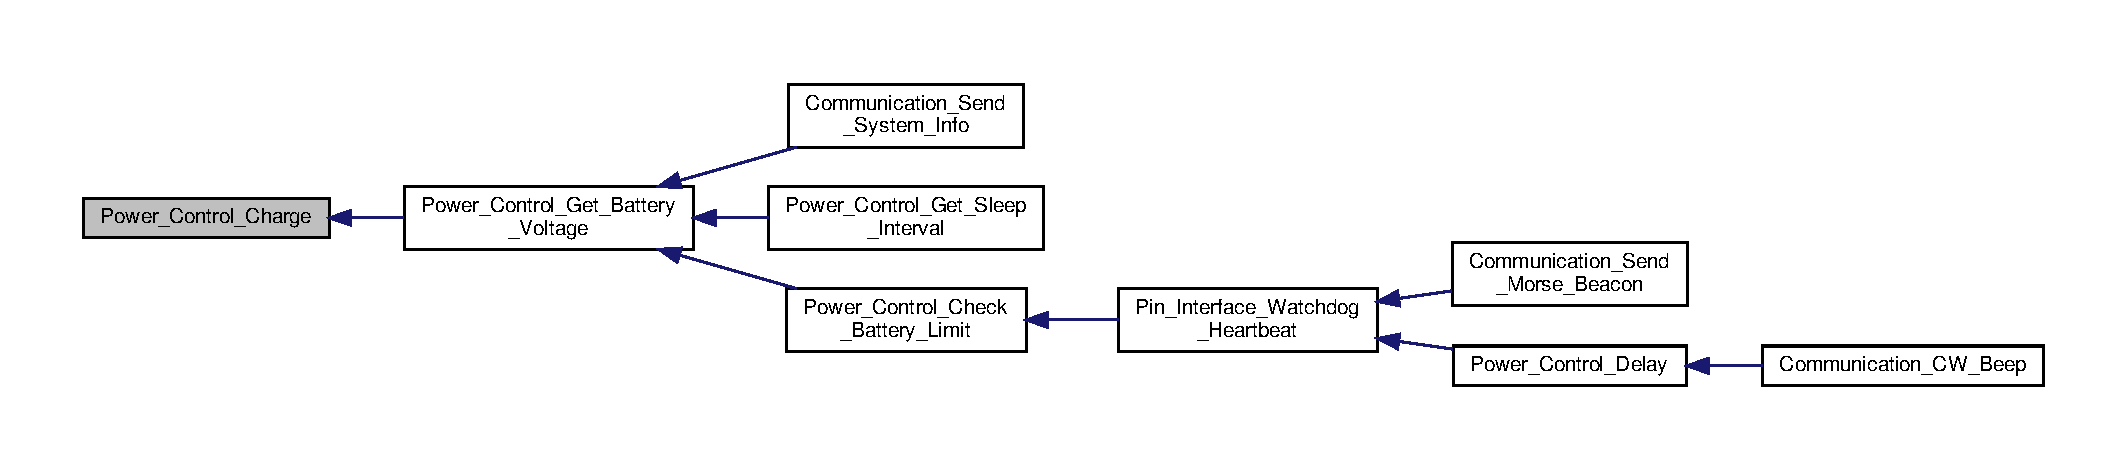
\includegraphics[width=350pt]{power__control_8h_a4e4e7a68a32a2d3fc0b7c0b14b391975_icgraph}
\end{center}
\end{figure}
\mbox{\Hypertarget{power__control_8h_a3dcf47e9ee8d130075c4466692810370}\label{power__control_8h_a3dcf47e9ee8d130075c4466692810370}} 
\index{power\+\_\+control.\+h@{power\+\_\+control.\+h}!Power\+\_\+\+Control\+\_\+\+Check\+\_\+\+Battery\+\_\+\+Limit@{Power\+\_\+\+Control\+\_\+\+Check\+\_\+\+Battery\+\_\+\+Limit}}
\index{Power\+\_\+\+Control\+\_\+\+Check\+\_\+\+Battery\+\_\+\+Limit@{Power\+\_\+\+Control\+\_\+\+Check\+\_\+\+Battery\+\_\+\+Limit}!power\+\_\+control.\+h@{power\+\_\+control.\+h}}
\subsubsection{\texorpdfstring{Power\+\_\+\+Control\+\_\+\+Check\+\_\+\+Battery\+\_\+\+Limit()}{Power\_Control\_Check\_Battery\_Limit()}}
{\footnotesize\ttfamily bool Power\+\_\+\+Control\+\_\+\+Check\+\_\+\+Battery\+\_\+\+Limit (\begin{DoxyParamCaption}{ }\end{DoxyParamCaption})}



Checks whether battery voltage is below low power limit. Will enable low power mode if that is the case. 

\begin{DoxyReturn}{Returns}
bool Whether battery check passed or not. 
\end{DoxyReturn}


Definition at line 169 of file power\+\_\+control.\+cpp.

Here is the call graph for this function\+:
\nopagebreak
\begin{figure}[H]
\begin{center}
\leavevmode
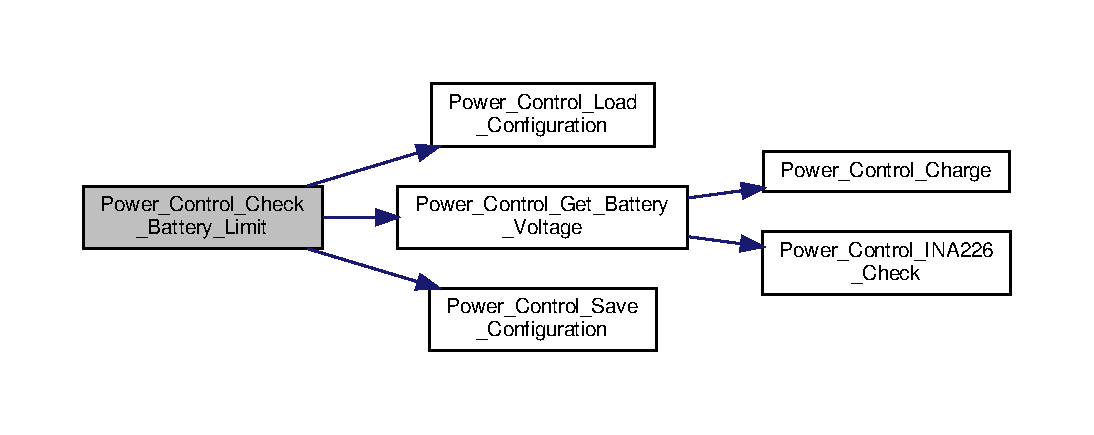
\includegraphics[width=350pt]{power__control_8h_a3dcf47e9ee8d130075c4466692810370_cgraph}
\end{center}
\end{figure}
Here is the caller graph for this function\+:
\nopagebreak
\begin{figure}[H]
\begin{center}
\leavevmode
\includegraphics[width=350pt]{power__control_8h_a3dcf47e9ee8d130075c4466692810370_icgraph}
\end{center}
\end{figure}
\mbox{\Hypertarget{power__control_8h_a3bff1402f7ac79b23628326e3fd7b560}\label{power__control_8h_a3bff1402f7ac79b23628326e3fd7b560}} 
\index{power\+\_\+control.\+h@{power\+\_\+control.\+h}!Power\+\_\+\+Control\+\_\+\+Delay@{Power\+\_\+\+Control\+\_\+\+Delay}}
\index{Power\+\_\+\+Control\+\_\+\+Delay@{Power\+\_\+\+Control\+\_\+\+Delay}!power\+\_\+control.\+h@{power\+\_\+control.\+h}}
\subsubsection{\texorpdfstring{Power\+\_\+\+Control\+\_\+\+Delay()}{Power\_Control\_Delay()}}
{\footnotesize\ttfamily void Power\+\_\+\+Control\+\_\+\+Delay (\begin{DoxyParamCaption}\item[{uint32\+\_\+t}]{ms,  }\item[{bool}]{sleep,  }\item[{bool}]{sleep\+Radio = {\ttfamily false} }\end{DoxyParamCaption})}



This function delays the program execution for the given number of milliseconds, while maintaining the watchdog signal to prevent it resetting. 

\begin{DoxyRefDesc}{Test}
\item[\hyperlink{test__test000043}{Test}](ID P\+O\+W\+E\+R\+\_\+\+C\+O\+N\+T\+\_\+\+H\+\_\+\+T8) (S\+EV 1) Check that the satellite\textquotesingle{}s program is delayed for the given number of seconds without restarting.\end{DoxyRefDesc}



\begin{DoxyParams}{Parameters}
{\em ms} & The amount of time to delay the program for. \\
\hline
{\em sleep} & Whether to use the Low\+Power libraries power\+Down feature. \\
\hline
{\em sleep\+Radio} & Whether to put the radio into sleep mode for the duration. \\
\hline
\end{DoxyParams}


Definition at line 73 of file power\+\_\+control.\+cpp.

Here is the call graph for this function\+:
\nopagebreak
\begin{figure}[H]
\begin{center}
\leavevmode
\includegraphics[width=350pt]{power__control_8h_a3bff1402f7ac79b23628326e3fd7b560_cgraph}
\end{center}
\end{figure}
Here is the caller graph for this function\+:
\nopagebreak
\begin{figure}[H]
\begin{center}
\leavevmode
\includegraphics[width=350pt]{power__control_8h_a3bff1402f7ac79b23628326e3fd7b560_icgraph}
\end{center}
\end{figure}
\mbox{\Hypertarget{power__control_8h_a6e2a22c1b8940caf3a89cf6f5e21e120}\label{power__control_8h_a6e2a22c1b8940caf3a89cf6f5e21e120}} 
\index{power\+\_\+control.\+h@{power\+\_\+control.\+h}!Power\+\_\+\+Control\+\_\+\+Get\+\_\+\+Battery\+\_\+\+Voltage@{Power\+\_\+\+Control\+\_\+\+Get\+\_\+\+Battery\+\_\+\+Voltage}}
\index{Power\+\_\+\+Control\+\_\+\+Get\+\_\+\+Battery\+\_\+\+Voltage@{Power\+\_\+\+Control\+\_\+\+Get\+\_\+\+Battery\+\_\+\+Voltage}!power\+\_\+control.\+h@{power\+\_\+control.\+h}}
\subsubsection{\texorpdfstring{Power\+\_\+\+Control\+\_\+\+Get\+\_\+\+Battery\+\_\+\+Voltage()}{Power\_Control\_Get\_Battery\_Voltage()}}
{\footnotesize\ttfamily float Power\+\_\+\+Control\+\_\+\+Get\+\_\+\+Battery\+\_\+\+Voltage (\begin{DoxyParamCaption}{ }\end{DoxyParamCaption})}



Get the battery voltage by switching the M\+P\+PT off and then on again after reading is taken. 

\begin{DoxyRefDesc}{Test}
\item[\hyperlink{test__test000046}{Test}](ID P\+O\+W\+E\+R\+\_\+\+C\+O\+N\+T\+\_\+\+H\+\_\+\+T11) (S\+EV 1) Check that this function returns the correct battery voltage.\end{DoxyRefDesc}


\begin{DoxyReturn}{Returns}
float The voltage returned by the I\+N\+A266 of the battery. 
\end{DoxyReturn}


Definition at line 139 of file power\+\_\+control.\+cpp.

Here is the call graph for this function\+:
\nopagebreak
\begin{figure}[H]
\begin{center}
\leavevmode
\includegraphics[width=350pt]{power__control_8h_a6e2a22c1b8940caf3a89cf6f5e21e120_cgraph}
\end{center}
\end{figure}
Here is the caller graph for this function\+:
\nopagebreak
\begin{figure}[H]
\begin{center}
\leavevmode
\includegraphics[width=350pt]{power__control_8h_a6e2a22c1b8940caf3a89cf6f5e21e120_icgraph}
\end{center}
\end{figure}
\mbox{\Hypertarget{power__control_8h_a38b1cf7d6af2bdccef1488666b05eda6}\label{power__control_8h_a38b1cf7d6af2bdccef1488666b05eda6}} 
\index{power\+\_\+control.\+h@{power\+\_\+control.\+h}!Power\+\_\+\+Control\+\_\+\+Get\+\_\+\+Charging\+\_\+\+Current@{Power\+\_\+\+Control\+\_\+\+Get\+\_\+\+Charging\+\_\+\+Current}}
\index{Power\+\_\+\+Control\+\_\+\+Get\+\_\+\+Charging\+\_\+\+Current@{Power\+\_\+\+Control\+\_\+\+Get\+\_\+\+Charging\+\_\+\+Current}!power\+\_\+control.\+h@{power\+\_\+control.\+h}}
\subsubsection{\texorpdfstring{Power\+\_\+\+Control\+\_\+\+Get\+\_\+\+Charging\+\_\+\+Current()}{Power\_Control\_Get\_Charging\_Current()}}
{\footnotesize\ttfamily float Power\+\_\+\+Control\+\_\+\+Get\+\_\+\+Charging\+\_\+\+Current (\begin{DoxyParamCaption}{ }\end{DoxyParamCaption})}



Gets the amperage which is being provided to the battery. 

\begin{DoxyRefDesc}{Test}
\item[\hyperlink{test__test000048}{Test}](ID P\+O\+W\+E\+R\+\_\+\+C\+O\+N\+T\+\_\+\+H\+\_\+\+T13) (S\+EV 1) Check the value returned by this function is the current charging solar panel Amperage.\end{DoxyRefDesc}


\begin{DoxyReturn}{Returns}
float The shunt current value of the I\+N\+A2256 
\end{DoxyReturn}


Definition at line 162 of file power\+\_\+control.\+cpp.

Here is the call graph for this function\+:
\nopagebreak
\begin{figure}[H]
\begin{center}
\leavevmode
\includegraphics[width=350pt]{power__control_8h_a38b1cf7d6af2bdccef1488666b05eda6_cgraph}
\end{center}
\end{figure}
Here is the caller graph for this function\+:
\nopagebreak
\begin{figure}[H]
\begin{center}
\leavevmode
\includegraphics[width=350pt]{power__control_8h_a38b1cf7d6af2bdccef1488666b05eda6_icgraph}
\end{center}
\end{figure}
\mbox{\Hypertarget{power__control_8h_ae60f6f685745e08c9ffbd6b6fbc025b9}\label{power__control_8h_ae60f6f685745e08c9ffbd6b6fbc025b9}} 
\index{power\+\_\+control.\+h@{power\+\_\+control.\+h}!Power\+\_\+\+Control\+\_\+\+Get\+\_\+\+Charging\+\_\+\+Voltage@{Power\+\_\+\+Control\+\_\+\+Get\+\_\+\+Charging\+\_\+\+Voltage}}
\index{Power\+\_\+\+Control\+\_\+\+Get\+\_\+\+Charging\+\_\+\+Voltage@{Power\+\_\+\+Control\+\_\+\+Get\+\_\+\+Charging\+\_\+\+Voltage}!power\+\_\+control.\+h@{power\+\_\+control.\+h}}
\subsubsection{\texorpdfstring{Power\+\_\+\+Control\+\_\+\+Get\+\_\+\+Charging\+\_\+\+Voltage()}{Power\_Control\_Get\_Charging\_Voltage()}}
{\footnotesize\ttfamily float Power\+\_\+\+Control\+\_\+\+Get\+\_\+\+Charging\+\_\+\+Voltage (\begin{DoxyParamCaption}{ }\end{DoxyParamCaption})}



Gets the charging voltage (from the solar panels) by not switching the M\+P\+PT off and taking an I\+N\+A226 reading. 

\begin{DoxyRefDesc}{Test}
\item[\hyperlink{test__test000047}{Test}](ID P\+O\+W\+E\+R\+\_\+\+C\+O\+N\+T\+\_\+\+H\+\_\+\+T12) (S\+EV 1) Check that this function returns the correct solar panel charging voltage.\end{DoxyRefDesc}


\begin{DoxyReturn}{Returns}
float The voltage provided by the solar panels. 
\end{DoxyReturn}


Definition at line 155 of file power\+\_\+control.\+cpp.

Here is the call graph for this function\+:
\nopagebreak
\begin{figure}[H]
\begin{center}
\leavevmode
\includegraphics[width=350pt]{power__control_8h_ae60f6f685745e08c9ffbd6b6fbc025b9_cgraph}
\end{center}
\end{figure}
Here is the caller graph for this function\+:
\nopagebreak
\begin{figure}[H]
\begin{center}
\leavevmode
\includegraphics[width=350pt]{power__control_8h_ae60f6f685745e08c9ffbd6b6fbc025b9_icgraph}
\end{center}
\end{figure}
\mbox{\Hypertarget{power__control_8h_aa26e5dcfde1aecf602a3a41ef6e205b8}\label{power__control_8h_aa26e5dcfde1aecf602a3a41ef6e205b8}} 
\index{power\+\_\+control.\+h@{power\+\_\+control.\+h}!Power\+\_\+\+Control\+\_\+\+Get\+\_\+\+Sleep\+\_\+\+Interval@{Power\+\_\+\+Control\+\_\+\+Get\+\_\+\+Sleep\+\_\+\+Interval}}
\index{Power\+\_\+\+Control\+\_\+\+Get\+\_\+\+Sleep\+\_\+\+Interval@{Power\+\_\+\+Control\+\_\+\+Get\+\_\+\+Sleep\+\_\+\+Interval}!power\+\_\+control.\+h@{power\+\_\+control.\+h}}
\subsubsection{\texorpdfstring{Power\+\_\+\+Control\+\_\+\+Get\+\_\+\+Sleep\+\_\+\+Interval()}{Power\_Control\_Get\_Sleep\_Interval()}}
{\footnotesize\ttfamily uint32\+\_\+t Power\+\_\+\+Control\+\_\+\+Get\+\_\+\+Sleep\+\_\+\+Interval (\begin{DoxyParamCaption}{ }\end{DoxyParamCaption})}



Get the amount of seconds to sleep for given the battery voltage. 

\begin{DoxyRefDesc}{Todo}
\item[\hyperlink{todo__todo000006}{Todo}]Julian -\/$>$ The sleep intervals should be updated to match the new C\+W-\/synced communications.\end{DoxyRefDesc}


\begin{DoxyRefDesc}{Test}
\item[\hyperlink{test__test000042}{Test}](ID P\+O\+W\+E\+R\+\_\+\+C\+O\+N\+T\+\_\+\+H\+\_\+\+T7) (S\+EV 1) Check what interval is returned at the designated voltages.\end{DoxyRefDesc}


\begin{DoxyReturn}{Returns}
uint32\+\_\+t The number of milliseconds to sleep for. 
\end{DoxyReturn}


Definition at line 47 of file power\+\_\+control.\+cpp.

Here is the call graph for this function\+:
\nopagebreak
\begin{figure}[H]
\begin{center}
\leavevmode
\includegraphics[width=350pt]{power__control_8h_aa26e5dcfde1aecf602a3a41ef6e205b8_cgraph}
\end{center}
\end{figure}
\mbox{\Hypertarget{power__control_8h_ac78b055f83071530eb3844378654db5e}\label{power__control_8h_ac78b055f83071530eb3844378654db5e}} 
\index{power\+\_\+control.\+h@{power\+\_\+control.\+h}!Power\+\_\+\+Control\+\_\+\+I\+N\+A226\+\_\+\+Check@{Power\+\_\+\+Control\+\_\+\+I\+N\+A226\+\_\+\+Check}}
\index{Power\+\_\+\+Control\+\_\+\+I\+N\+A226\+\_\+\+Check@{Power\+\_\+\+Control\+\_\+\+I\+N\+A226\+\_\+\+Check}!power\+\_\+control.\+h@{power\+\_\+control.\+h}}
\subsubsection{\texorpdfstring{Power\+\_\+\+Control\+\_\+\+I\+N\+A226\+\_\+\+Check()}{Power\_Control\_INA226\_Check()}}
{\footnotesize\ttfamily bool Power\+\_\+\+Control\+\_\+\+I\+N\+A226\+\_\+\+Check (\begin{DoxyParamCaption}{ }\end{DoxyParamCaption})}



Check that the I\+N\+A2256 is valid. 

\begin{DoxyRefDesc}{Test}
\item[\hyperlink{test__test000045}{Test}](ID P\+O\+W\+E\+R\+\_\+\+C\+O\+N\+T\+\_\+\+H\+\_\+\+T10) (S\+EV 1) Check that this function correctly returns the state of the I\+N\+A226 component.\end{DoxyRefDesc}


\begin{DoxyReturn}{Returns}
true The I\+N\+A226 is working correctly. 

false The I\+N\+A226 is not working correctly. 
\end{DoxyReturn}


Definition at line 114 of file power\+\_\+control.\+cpp.

Here is the caller graph for this function\+:
\nopagebreak
\begin{figure}[H]
\begin{center}
\leavevmode
\includegraphics[width=350pt]{power__control_8h_ac78b055f83071530eb3844378654db5e_icgraph}
\end{center}
\end{figure}
\mbox{\Hypertarget{power__control_8h_a67027a313959753703a50352ee41b109}\label{power__control_8h_a67027a313959753703a50352ee41b109}} 
\index{power\+\_\+control.\+h@{power\+\_\+control.\+h}!Power\+\_\+\+Control\+\_\+\+Load\+\_\+\+Configuration@{Power\+\_\+\+Control\+\_\+\+Load\+\_\+\+Configuration}}
\index{Power\+\_\+\+Control\+\_\+\+Load\+\_\+\+Configuration@{Power\+\_\+\+Control\+\_\+\+Load\+\_\+\+Configuration}!power\+\_\+control.\+h@{power\+\_\+control.\+h}}
\subsubsection{\texorpdfstring{Power\+\_\+\+Control\+\_\+\+Load\+\_\+\+Configuration()}{Power\_Control\_Load\_Configuration()}}
{\footnotesize\ttfamily void Power\+\_\+\+Control\+\_\+\+Load\+\_\+\+Configuration (\begin{DoxyParamCaption}{ }\end{DoxyParamCaption})}



Load the configuration bytes from the E\+E\+P\+R\+OM into R\+AM. 

\begin{DoxyRefDesc}{Test}
\item[\hyperlink{test__test000039}{Test}](ID P\+O\+W\+E\+R\+\_\+\+C\+O\+N\+T\+\_\+\+H\+\_\+\+T0) (S\+EV 1) Make sure that the power configuration is loaded from E\+E\+P\+R\+OM correctly.\end{DoxyRefDesc}


Definition at line 15 of file power\+\_\+control.\+cpp.

Here is the caller graph for this function\+:
\nopagebreak
\begin{figure}[H]
\begin{center}
\leavevmode
\includegraphics[width=350pt]{power__control_8h_a67027a313959753703a50352ee41b109_icgraph}
\end{center}
\end{figure}
\mbox{\Hypertarget{power__control_8h_a18bd8cf80280cfba12636778283abf78}\label{power__control_8h_a18bd8cf80280cfba12636778283abf78}} 
\index{power\+\_\+control.\+h@{power\+\_\+control.\+h}!Power\+\_\+\+Control\+\_\+\+Save\+\_\+\+Configuration@{Power\+\_\+\+Control\+\_\+\+Save\+\_\+\+Configuration}}
\index{Power\+\_\+\+Control\+\_\+\+Save\+\_\+\+Configuration@{Power\+\_\+\+Control\+\_\+\+Save\+\_\+\+Configuration}!power\+\_\+control.\+h@{power\+\_\+control.\+h}}
\subsubsection{\texorpdfstring{Power\+\_\+\+Control\+\_\+\+Save\+\_\+\+Configuration()}{Power\_Control\_Save\_Configuration()}}
{\footnotesize\ttfamily void Power\+\_\+\+Control\+\_\+\+Save\+\_\+\+Configuration (\begin{DoxyParamCaption}{ }\end{DoxyParamCaption})}



Saves the configuration bytes from R\+AM into E\+E\+P\+R\+OM. 

\begin{DoxyRefDesc}{Test}
\item[\hyperlink{test__test000040}{Test}](ID P\+O\+W\+E\+R\+\_\+\+C\+O\+N\+T\+\_\+\+H\+\_\+\+T1) (S\+EV 1) Make sure that the power configuration is wrote to the E\+E\+P\+R\+OM correctly.\end{DoxyRefDesc}


Definition at line 19 of file power\+\_\+control.\+cpp.

Here is the caller graph for this function\+:
\nopagebreak
\begin{figure}[H]
\begin{center}
\leavevmode
\includegraphics[width=350pt]{power__control_8h_a18bd8cf80280cfba12636778283abf78_icgraph}
\end{center}
\end{figure}
\mbox{\Hypertarget{power__control_8h_af06e9b8ca5da269e5b0bf31debe17740}\label{power__control_8h_af06e9b8ca5da269e5b0bf31debe17740}} 
\index{power\+\_\+control.\+h@{power\+\_\+control.\+h}!Power\+\_\+\+Control\+\_\+\+Setup\+\_\+\+I\+N\+A226@{Power\+\_\+\+Control\+\_\+\+Setup\+\_\+\+I\+N\+A226}}
\index{Power\+\_\+\+Control\+\_\+\+Setup\+\_\+\+I\+N\+A226@{Power\+\_\+\+Control\+\_\+\+Setup\+\_\+\+I\+N\+A226}!power\+\_\+control.\+h@{power\+\_\+control.\+h}}
\subsubsection{\texorpdfstring{Power\+\_\+\+Control\+\_\+\+Setup\+\_\+\+I\+N\+A226()}{Power\_Control\_Setup\_INA226()}}
{\footnotesize\ttfamily void Power\+\_\+\+Control\+\_\+\+Setup\+\_\+\+I\+N\+A226 (\begin{DoxyParamCaption}{ }\end{DoxyParamCaption})}



Initializes the I\+N\+A226 current sensor. 

\begin{DoxyRefDesc}{Test}
\item[\hyperlink{test__test000044}{Test}](ID P\+O\+W\+E\+R\+\_\+\+C\+O\+N\+T\+\_\+\+H\+\_\+\+T9) (S\+EV 1) Check that the I\+N\+A226 is configured ok.\end{DoxyRefDesc}


Definition at line 108 of file power\+\_\+control.\+cpp.


\hypertarget{system__info_8h}{}\section{Fossa\+Sat1\+B/system\+\_\+info.h File Reference}
\label{system__info_8h}\index{Fossa\+Sat1\+B/system\+\_\+info.\+h@{Fossa\+Sat1\+B/system\+\_\+info.\+h}}
{\ttfamily \#include \char`\"{}Fossa\+Sat1\+B.\+h\char`\"{}}\newline
Include dependency graph for system\+\_\+info.\+h\+:
\nopagebreak
\begin{figure}[H]
\begin{center}
\leavevmode
\includegraphics[width=350pt]{system__info_8h__incl}
\end{center}
\end{figure}
This graph shows which files directly or indirectly include this file\+:
\nopagebreak
\begin{figure}[H]
\begin{center}
\leavevmode
\includegraphics[width=350pt]{system__info_8h__dep__incl}
\end{center}
\end{figure}
\subsection*{Functions}
\begin{DoxyCompactItemize}
\item 
void \hyperlink{system__info_8h_a51295b55492a253ad9c695525c40d458}{System\+\_\+\+Info\+\_\+\+Set\+\_\+\+Callsign} (char $\ast$new\+Callsign)
\begin{DoxyCompactList}\small\item\em Set the callsign to be used for each transmission to E\+E\+P\+R\+OM. \end{DoxyCompactList}\item 
void \hyperlink{system__info_8h_a4ba2aee682a65d201b020b7fcf20939c}{System\+\_\+\+Info\+\_\+\+Get\+\_\+\+Callsign} (char $\ast$buff, uint8\+\_\+t len)
\begin{DoxyCompactList}\small\item\em Gets the callsign which is current set in E\+E\+P\+R\+OM. \end{DoxyCompactList}\end{DoxyCompactItemize}


\subsection{Detailed Description}
\begin{DoxyRefDesc}{Todo}
\item[\hyperlink{todo__todo000007}{Todo}]this module should contain the Restart Counter logic. \end{DoxyRefDesc}


\subsection{Function Documentation}
\mbox{\Hypertarget{system__info_8h_a4ba2aee682a65d201b020b7fcf20939c}\label{system__info_8h_a4ba2aee682a65d201b020b7fcf20939c}} 
\index{system\+\_\+info.\+h@{system\+\_\+info.\+h}!System\+\_\+\+Info\+\_\+\+Get\+\_\+\+Callsign@{System\+\_\+\+Info\+\_\+\+Get\+\_\+\+Callsign}}
\index{System\+\_\+\+Info\+\_\+\+Get\+\_\+\+Callsign@{System\+\_\+\+Info\+\_\+\+Get\+\_\+\+Callsign}!system\+\_\+info.\+h@{system\+\_\+info.\+h}}
\subsubsection{\texorpdfstring{System\+\_\+\+Info\+\_\+\+Get\+\_\+\+Callsign()}{System\_Info\_Get\_Callsign()}}
{\footnotesize\ttfamily void System\+\_\+\+Info\+\_\+\+Get\+\_\+\+Callsign (\begin{DoxyParamCaption}\item[{char $\ast$}]{buff,  }\item[{uint8\+\_\+t}]{len }\end{DoxyParamCaption})}



Gets the callsign which is current set in E\+E\+P\+R\+OM. 

\begin{DoxyRefDesc}{Todo}
\item[\hyperlink{todo__todo000008}{Todo}]Implement a R\+AM variable to hold this since E\+E\+P\+R\+OM degrades with use, memory restrictions do not allow this to be alloced in R\+AM.\end{DoxyRefDesc}


\begin{DoxyRefDesc}{Test}
\item[\hyperlink{test__test000050}{Test}](ID S\+Y\+S\+\_\+\+I\+N\+F\+\_\+\+T1) (S\+EV 1) Make sure that the callsign is retrieved correctly from E\+E\+P\+R\+OM.\end{DoxyRefDesc}



\begin{DoxyParams}{Parameters}
{\em buff} & The destination for the callsign. \\
\hline
{\em len} & The length of the callsign. \\
\hline
\end{DoxyParams}


Definition at line 21 of file system\+\_\+info.\+cpp.

Here is the caller graph for this function\+:
\nopagebreak
\begin{figure}[H]
\begin{center}
\leavevmode
\includegraphics[width=350pt]{system__info_8h_a4ba2aee682a65d201b020b7fcf20939c_icgraph}
\end{center}
\end{figure}
\mbox{\Hypertarget{system__info_8h_a51295b55492a253ad9c695525c40d458}\label{system__info_8h_a51295b55492a253ad9c695525c40d458}} 
\index{system\+\_\+info.\+h@{system\+\_\+info.\+h}!System\+\_\+\+Info\+\_\+\+Set\+\_\+\+Callsign@{System\+\_\+\+Info\+\_\+\+Set\+\_\+\+Callsign}}
\index{System\+\_\+\+Info\+\_\+\+Set\+\_\+\+Callsign@{System\+\_\+\+Info\+\_\+\+Set\+\_\+\+Callsign}!system\+\_\+info.\+h@{system\+\_\+info.\+h}}
\subsubsection{\texorpdfstring{System\+\_\+\+Info\+\_\+\+Set\+\_\+\+Callsign()}{System\_Info\_Set\_Callsign()}}
{\footnotesize\ttfamily void System\+\_\+\+Info\+\_\+\+Set\+\_\+\+Callsign (\begin{DoxyParamCaption}\item[{char $\ast$}]{new\+Callsign }\end{DoxyParamCaption})}



Set the callsign to be used for each transmission to E\+E\+P\+R\+OM. 

\begin{DoxyRefDesc}{Test}
\item[\hyperlink{test__test000049}{Test}](ID S\+Y\+S\+\_\+\+I\+N\+F\+\_\+\+T0) (S\+EV 1) Make sure this function writes the callsign to E\+E\+P\+R\+OM.\end{DoxyRefDesc}



\begin{DoxyParams}{Parameters}
{\em new\+Callsign} & String containing the new callsign to use. \\
\hline
\end{DoxyParams}


Definition at line 3 of file system\+\_\+info.\+cpp.


%--- End generated contents ---

% Index
\backmatter
\newpage
\phantomsection
\clearemptydoublepage
\addcontentsline{toc}{chapter}{Index}
\printindex

\end{document}
